% v1 paper of the frozen-encoder study, assembled 20 Nov 2026 from the reviewed drafts in
% Drive fm_v1/draft/2026-11-19/ (intro.md, methods_results_v2.md, discussion.md, claim_ledger.md)
% and the R2 development spread. Template: docs/report/fm_ieee/main.tex (tag fm-proposal-s1).
% Build from this directory: tectonic --keep-logs main.tex
%
% Source keys in "% src:" comments (as in the drafts):
%   PR  = protocols.md. Line numbers are those of commit 50a03dc (the drafts' base); at HEAD 24da8f3,
%         lines 256-439 move +2 and lines from 440 move +16 (R2 rule row and the 19 Nov
%         "after the draft review" entry were added).
%   AM  = docs/research/FM_AMENDMENTS.md; FP = docs/research/FM_PROTOCOL.md
%   WR  = docs/report/2026-11-14_weekly_report.tex
%   ARC = D:/Few-shot/drive/fm_v1/final/final-20261113T170804Z/evaluation/results-20261114T093033Z.zip
%   LOCK= D:/Few-shot/drive/fm_v1/final/final-20261113T170804Z/input-lock.zip
%   DRV = D:/Few-shot/drive/fm_v1/final/final-20261113T170804Z/ (step11_pilots.txt, step14_external.txt)
%   PR@fec827e = protocols.md at commit fec827e (21 Nov), used for the P10 and E1-E4 text added on 21 Nov:
%         P10 rule row l.254; change log 20 Nov l.460-484, 21 Nov (P10) l.485-498; subsection
%         "Phase-1 controls E1-E4" l.505-605 (shared rules l.514-545, E0 l.547-584, E1-E4 rows l.587-590,
%         GPU plan and drop order l.592-601, default placement l.603-605).
%   DEV = docs/research/FM_DEVIATIONS.md (D1: OCTID size not constant)
%   PH  = results/fm_v1/posthoc/ (post hoc; every row labelled); R2 = PH R2_development_spread.csv
%   P10 files (PH): P10_screen_summary.csv, P10_screen_synthetic.csv, P10_review_key.csv, P10_review_marks.csv,
%         P10_matched_pairs.csv, P10_sensitivity.csv (line numbers count the header as line 1)
%   E CSVs: written by fm_posthoc.py e1-e4 into PH (none exists on 21 Nov); tables/e*.tex are generated from
%         them by make_tables.py and shown only when present (\havetable below)
%   HP  = results/fm_v1/posthoc/pre_rule/2026-11-18/fable_holdout_plan.md, section D (adopted wording)
%   LS  = docs/research/lit-scan-gan-vs-basic.md; CX = docs/research/CONTEXT.md
%   M/I/D = methods_results_v2.md / intro.md / discussion.md (draft, with their own source comments)
% Rounding: three decimals, half up from the shortest decimal form (0.7265 -> 0.727, 0.7725 -> 0.773);
% agent default recorded in PR (HEAD) 19 Nov "after the draft review". Tables: make_tables.py.
\documentclass[conference]{IEEEtran}
\usepackage[T1]{fontenc}
\usepackage{cite}
\usepackage{amsmath,amssymb}
\usepackage{graphicx,booktabs,array,makecell,longtable}
\usepackage{xurl}
\usepackage[hidelinks]{hyperref}
\hypersetup{pdftitle={Frozen Foundation Models for Few-Shot Rare Retinal OCT Classification: A Pre-Registered, Shortcut-Audited Evaluation},pdfauthor={Doan Tung Lam, Ha Quang Minh, Pham Duc Anh, Ngo Hoang Phuc}}
\newcommand{\todo}[1]{\textbf{[TODO: #1]}}
\newcommand{\fnRS}{\textsuperscript{a}}
\renewcommand\theadfont{\normalsize}
% Phase-1 (E1-E4) tables: \havetable{name}\ifgen ... \fi typesets a block only if tables/name.tex exists,
% i.e. only after make_tables.py has read the E CSVs that fm_posthoc.py writes. No E result exists on 21 Nov.
\newif\ifgen
\newcommand{\havetable}[1]{\IfFileExists{tables/#1.tex}{\gentrue}{\genfalse}}
% IEEEtran.bst's documented control-entry citation avoids a printed reference.
\makeatletter
\def\bstctlcite{\@ifnextchar[{\@bstctlcite}{\@bstctlcite[@auxout]}}
\def\@bstctlcite[#1]#2{\@bsphack
  \@for\@citeb:=#2\do{%
    \edef\@citeb{\expandafter\@firstofone\@citeb}%
    \if@filesw\immediate\write\csname #1\endcsname{\string\citation{\@citeb}}\fi}%
  \@esphack}
\makeatother
\begin{document}
\bstctlcite{IEEEcontrol}
\title{Image Size Alone Beats Frozen Foundation Models at One Shot: A Pre-Registered Audit of a Rare Retinal OCT Benchmark}
% src: title kept as drafted (PR change log 24 Nov: Lam delegated the remaining Phase-1 choices); finding-led title, PR change log "22 Nov, framing approved" ("The title leads with the finding") and the mentor's review of 23 Nov (docs/research/MENTOR_LEARNING_LOG.md, Feedback 3); the finding: ARC size_only_reference.csv line 2 (0.578 at K=1, above every model); earlier title: PR l.33-34 and l.430-432 (Lam, 19 Nov)
\author{\IEEEauthorblockN{Doan Tung Lam, Ha Quang Minh, Pham Duc Anh, Ngo Hoang Phuc}
\IEEEauthorblockA{National Economics University}}
\maketitle

\begin{abstract}
Rare retinal diseases have few labelled optical coherence tomography (OCT) images, so their benchmarks are assembled from many sources, while frozen foundation models promise to classify them from a handful of examples. We ask whether few-shot scores on such a benchmark measure the disease or the image source. We report a pre-registered audit of three frozen foundation models (MIRAGE, DINOv2, RETFound) and frozen ImageNet Inception-v3 on the public five-class rare-disease benchmark of Yoo et al.\ (124 development and 22 hold-out images), with identical supports ($K=1$--8 per class, 100 draws) and cosine prototypes; the protocol and inputs were hashed before any score. A rule that sees only image width and height scored 0.578 at $K=1$, above all four models (best: MIRAGE, 0.495; unpaired means). MIRAGE had the highest development macro recall averaged over $K$ (0.650; Inception-v3 0.534). The remaining results are post hoc, each under a rule committed before its numbers. Under a size and framing control, MIRAGE's lead over Inception-v3 fell from 0.116 to 0.063, with a 5th percentile over support draws of 0.0025 (95 of 100 draws above 0; the uncertainty of this percentile was not estimated). Within a fixed preprocessing grid MIRAGE stayed ahead, while one normalisation constant moved RETFound from 0.406 to 0.578. External false-rare counts changed with the input recipe: the control moved MIRAGE's OCTDL normal scans called rare from 30 to 261 of 332, and single preprocessing changes moved 10 of 20 counts outside their locked intervals. A few-shot test told normal scans from three sources apart above chance at every $K$ (two-way macro recall at least 0.67 at $K=1$; chance 0.50). Four of the 22 hold-out images have a same-picture copy among the development images, which the locked duplicate screen did not flag. We therefore report rankings beside size, framing and source controls, and false-rare rates per recipe. The results describe web-collected images and published labels; they make no clinical claim.
\end{abstract}
% src: 124/22 PR l.54-55; lock PR l.5-11, l.183; K and draws PR l.127-128; 0.650/0.534 ARC nomination.json; size-only 0.578 at K=1 above every model ARC size_only_reference.csv line 2 (MIRAGE K=1 0.4948: PH E1b_development.csv line 42); E1: PH E1d_success.csv (E1-M 0.063136, locked 0.115770, p05 0.002519, draws_above_0 95); hold-out copies: PH P10_matched_pairs.csv (5 development--hold-out pairs, 4 hold-out images: MacTel/19, RP/17, RP/20, Stargardt/03; Section IV-F, P10); question and order: PR change log "22 Nov, framing approved", mentor's review of 23 Nov; E3: PH E3_criteria.csv (1) and (2), E3_development.csv (RETFound R-norm05 0.578, locked 0.406); E1g_nine_way.csv (MIRAGE OCTDL NORMAL locked 30, E1-M 261 of 332); E3_criteria.csv (3) (10 of 20 outside); E4a_fewshot_source_test.csv (normal-only pairs, 24 model cells per K; lowest K=1 mean 0.6743, DINOv2 locked, Kermany vs OCTDL, p05 0.516; lowest cell at K=2, 4, 8: 0.755, 0.810, 0.877); "uncertainty not estimated": PR change log "22 Nov, pre-freeze double-check"; wording approved verdicts PR@77d16a4 "Phase-1 verdicts" (summary line). Draft 21 Nov, audit-led 23 Nov; kept 24 Nov (PR change log 24 Nov).
\begin{IEEEkeywords}
optical coherence tomography, rare retinal disease, few-shot learning, frozen encoders, foundation models, shortcut learning, pre-registration
\end{IEEEkeywords}

\section{Introduction}
\label{sec:intro}
Some retinal diseases have very few labelled OCT images. Here ``rare'' means label scarcity within a dataset, not prevalence in patients. A class is rare when it holds at most 5\% of its dataset's labelled images, and few-shot when the pool its examples are drawn from holds at most 30 labelled images.
% src: PR l.355-358 (B1, 18 Nov), l.378-379
The five classes of the public benchmark of Yoo et al.\ \cite{Yoo2021} are both: central serous chorioretinopathy (CSC), macular hole (MH), macular telangiectasia (MacTel), Stargardt disease and retinitis pigmentosa (RP). Each class has 23 to 32 images, 0.55--0.77\% of the 4,146 labelled images this study used (our own subsample of 4,000 Kermany images plus the 146 rare images). Development pools hold 19 to 27 images.
% src: PR l.360-363; PR l.54; ARC reports/geometry/MIRAGE/geometry_summary.csv lines 2, 4, 6, 8 (Kermany fitting n = 1000 per class). Denominator kept as in PR (C9; FP l.273 counts 5,146 per encoder) -- agent default, see README
Pools this small leave few images to train a classifier and fewer to test one.

Frozen pretrained encoders offer another route. Each image becomes a feature vector, each class becomes the mean of a few labelled examples, and a new image takes the nearest class. SimpleShot showed that nearest-centroid classification on fixed features is a serious few-shot baseline at several $K$ \cite{SimpleShot2019}; our rule is of that kind, without its centring step.
% src: PR l.493 (SimpleShot, section 10); AM l.316; LITERATURE_KB l.244; PR l.320 (centring dropped)
RETFound \cite{RETFound2023} and MIRAGE \cite{MIRAGE2025} were pretrained on retinal images; DINOv2 \cite{DINOv2} learned general-purpose features from everyday images. MIRAGE compared the same kinds of encoder, but with classifiers trained on each full dataset \cite{MIRAGE2025}.
% src: PR l.41-46; PR l.30-31; AM l.310

A small benchmark built from many sources also invites shortcuts: a model can sort images by how they were acquired, cropped or stored, rather than by the retina. In chest radiography, convolutional networks identified the hospital system a film came from, which may confound predictions \cite{Zech2018}.
% src: Zech et al. 2018, PLOS Medicine 15(11):e1002683, abstract: "CNNs robustly identified hospital system and department within a hospital, which can have large differences in disease burden and may confound predictions" (publisher page read 24 Nov 2026); the one shortcut-learning source, added to PR section 10 on 24 Nov
Yoo et al.\ collected the rare images by web search; they carry no patient identifiers \cite{Yoo2021}.
% src: Yoo PMC7829497 ("Google Images and Google search engine"); PR l.381-383; HP D(3)
Before our input lock, a rule that used only file width and height reached a leave-one-out macro recall of 0.659 on the 124 development images (chance 0.20). The same pre-lock check also scored the 22 hold-out images.
% src: docs/research/FM_RULE_TRACKER.md l.26 (N-1); docs/research/fm_independent_review/FM_INDEPENDENT_REVIEW.md l.82-85 (0.659); AM l.65-67 (disclosure)
The rare images also have wide flat borders. In the locked geometry table, the median share of the image in flat border rows and columns is 0.34 to 0.50 per rare class among development images; for Kermany, OCTID and OCTDL it is at most 0.002 per class.
% src: ARC reports/geometry/MIRAGE/geometry_summary.csv border_share_median lines 15, 17, 19, 21, 23 (0.339-0.502) and lines 2-14 (0.0; Kermany DME fitting 0.00195)
In our earlier replication, rare and common images were almost linearly separable in frozen Inception-v3 features. Disease and source were confounded, so that test could not say which of the two the features read.
% src: CX l.117, l.132-134

This raises a question for any classifier that includes these classes: how often does it call normal scans from other sources ``rare''? None of the four studies we compared when the protocol was written (Yoo et al.\ \cite{Yoo2021}, RETFound \cite{RETFound2023}, MIRAGE \cite{MIRAGE2025} and a 2026 external validation on OCTID \cite{TVST2026}) measured this.
% src: AM l.297-314 (A3 precedent table, 13 Nov; l.313)

This paper is a pre-registered audit of a public rare-OCT benchmark, carried out through a comparison of frozen foundation models. Its question is whether few-shot scores on such a benchmark measure the disease or the image source.
% src: PR l.33-34, l.430-432 (Lam, 19 Nov; mentor to confirm 23 Nov)
Its aim is less to find the best backbone than to measure how the four encoders' results change across support draws, input recipes and image sources, beside references that see no retina (image size, a thumbnail). The comparison of models was registered first; the audit framing was adopted after the locked results were known, and every analysis added after the lock is labelled post hoc with the date of its rule.
% src: framing only, no new number; mentor request of 20 Nov and review of 23 Nov (docs/research/MENTOR_LEARNING_LOG.md, Feedbacks 2 and 3); PR change log "22 Nov, framing approved"; post hoc labelling: PR section 8, S5 rule 2 and Phase-1 shared rule 2
We compare MIRAGE, RETFound and DINOv2 with frozen ImageNet Inception-v3, the backbone family of Yoo et al., at 1 to 8 labelled images per disease in development and up to 16 on the hold-out. Beside the five-way task, a nine-way audit adds the four common Kermany classes \cite{Kermany2018} and counts normal scans from other sources called rare. Our contributions are three.
% src: PR l.35-36, l.92, l.127-128, l.140-141; PR l.423-425 (wording); PR l.23-25
\begin{enumerate}
\item \textbf{A shortcut audit.} A size-only reference, which sees no pixel, sits beside every model and every $K$; at $K=1$ it scored 0.578, above all four models. A model at or below it has not shown that it reads the retina. Passing it is necessary, not sufficient: the audit measures some acquisition cues and removes none. The false-rare rate on normal scans is reported for Kermany, OCTID and OCTDL separately, each beside the share of the same sources' disease images that the head calls any rare class. For OCTID and OCTDL disease images we report agreement with the published labels only.
% src: AM l.97-101 (A2 N-1); PR l.104; AM l.41, l.48-50; PR l.140-143; PR l.256 (R1); PR l.83-84
\item \textbf{A pre-registered comparison on identical supports.} The protocol was frozen on 5 November 2026 and amended three times, each dated (A1 on 12 November, A2 and A3 on 13 November), before the input lock of 13 November. Rosters, episodes, models, code and rules were hashed into that lock, and the hashes were deposited on Zenodo; the approval of the lock, recorded before the first scoring file was written, already cites the deposit as published (Section~\ref{sec:design}). One model was nominated from the development folds only and sealed before any model of this study was scored on a hold-out or external image. Two earlier looks are disclosed: our October replication had scored the 22 hold-out images, and the pre-lock size check above used the labels of the development and hold-out images. Every model saw the same support images at $K=1$, 2, 4 and 8 per class, drawn 100 times, and is read against Inception-v3 on the same draws.
% src: PR l.5-11; AM l.7, l.56, l.168; PR l.183; ARC approvals.json (recorded_utc 2026-11-14T09:11:48, "published 2026-11-14"); PR l.136-140, l.184; PR l.55-56; PR l.245 (October heads 17/18/19 of 22); AM l.65-67; PR l.127-128
\item \textbf{The provenance of the public release.} The release we used holds 146 images, not the 119 of the original paper; a post hoc same-picture audit found that four of our 22 hold-out images have a copy among the development images, and the locked duplicate screen flagged none of them (Sections~\ref{sec:methods} and~\ref{sec:res-posthoc}). We state what our numbers can and cannot be compared with (Section~\ref{sec:related}). All planned results are released, favourable or not.
% src: PR l.59-67 (v1 119 images, v2 146); PH P10_matched_pairs.csv (4 hold-out images in 5 development--hold-out pairs) and P10 text in Section IV-F ("The locked duplicate screen had flagged none of the 14 pairs"); PR l.421-427; AM l.192-193 (A1 rule 6); development spread filled by R2 (PR HEAD l.256-257); item order (audit first) and plain wording: PR change log "22 Nov, framing approved", rebuttal of 23 Nov (MENTOR_LEARNING_LOG.md)
\end{enumerate}

MIRAGE was nominated. Its development macro recall, averaged over $K=1$, 2, 4 and 8, was 0.650 (the score it was nominated on, which the locked file calls optimistic), against 0.534 for Inception-v3.
% src: ARC reports/nomination/nomination.json arms.MIRAGE.score 0.6497, arms.Inception.score 0.5339; "interpretation": "prespecified allocation rule; selected development score is optimistic"
Image size alone scored 0.578 at $K=1$, a higher mean than every model; MIRAGE's mean was higher from $K=2$ (unpaired means; no paired model-minus-size-only row exists). RETFound stayed below the size-only reference at every $K$. DINOv2 and Inception-v3 passed it only at $K=4$ and 8, and the size-only mean over $K$ (0.569) is above both of their means (0.558 and 0.534).
% src: ARC size_only_reference.csv lines 2-6 (0.578, 0.550, 0.560, 0.589; mean 0.569); nomination.json k_scores
With its locked recipe on the published, frame-filling inputs, MIRAGE called 0 of 169 patient-disjoint Kermany normal scans rare, 4 of 206 OCTID and 30 of 332 OCTDL. Beside these, the same head called 41 of 102 OCTID CSC images and 11 of 102 OCTID MH images any rare class, and 3 of 39 OCTDL MH images (post hoc, R1). It called only 26 of the 332 OCTDL normal scans normal. Other models' false-rare rates, some lower than MIRAGE's, are in Section~\ref{sec:res-frr}.
% src: ARC external_source_audit.csv lines 38, 52, 49, 50; PH R1_rare_beside_false_rare.csv lines 11-13; qualifier PR l.418-419; lower rates: same file lines 67 (Inception OCTDL 11) and 16 (RETFound OCTID 0)
On the 22 hold-out images, the nine-way head named 20 correctly for MIRAGE and 13 for Inception-v3; with four or five images per class, these counts show direction only.
% src: ARC external_source_audit.csv Kermany recall_<rare class> numerators (Table III); WR l.288-291; HP D(1)

\section{Related Work}
\label{sec:related}
\textbf{Rare OCT diseases on this benchmark.} Yoo et al.\ \cite{Yoo2021} trained a nine-way classifier on Inception-v3 features, with per-disease CycleGANs that turned normal scans into rare-disease images; they also tried a prototypical network, a Siamese network and nearest neighbours. They reported 92.1\% accuracy on an independent test and 93.9\% in five-fold cross-validation, for a classifier trained on every rare training image plus generated ones; most test images were common classes. Their test files are not public, and the public release changed after submission (version 1, 27 March 2020, 119 images; version 2, 29 October 2020, 146 images, which we use). Their figures are therefore context, not a baseline.
% src: Yoo PMC7829497 (Tables 2, 3; prototypical, Siamese, KNN); HP D(2), adopted PR l.421-427; "every rare training image" PR l.110-111 (agent default, PR HEAD 19 Nov entry); version dates pre_rule/2026-11-18/md_versions.json; "after submission": Yoo article history (received 15 Apr 2020, accepted 15 Jan 2021; claim ledger X5, M94)
Our 22-image hold-out matches the class counts of the test in Yoo et al.; which images they tested on was never published. It was inspected in our earlier work, so it is not blind, and we read it for direction only.
% src: HP D(1), adopted PR l.421-424; PR l.55-58

Later work reusing these images did not rebuild that test either. Sun et al.\ \cite{Sun2024} drew repeated five-way $K$-shot tasks ($K=1$, 3, 5) from the rare images with a trained network. Our development protocol resembles that design, with frozen encoders, grouped folds and 100 paired draws. Pools, draws and training differ, so we do not rank our results against theirs. We found Sun et al.\ on 18 November, after the lock; the registered amendment A3 still lists $K$-shot evaluation on these images as a gap, which we correct here.
% src: LS l.149-154; PR l.32-33, l.498; HP D(2); "resembles" agent default (PR HEAD 19 Nov entry); AM l.310-311
Tai et al.\ \cite{Tai2025} re-implemented the pipeline of Yoo et al.\ and set their five-fold cross-validation accuracy (93.76\%) beside Yoo's 93.9\%. They also report per-class rates on an independent test that the paper does not define. We avoid such comparisons.
% src: LS l.102, l.137; PR l.499

\textbf{Frozen encoders and few-shot classification.} MIRAGE \cite{MIRAGE2025} compared supervised ImageNet pretraining, DINOv2, RETFound and itself with linear probes on full datasets, including Kermany, OCTID and OCTDL; its balanced accuracy is the same quantity as our macro recall. Pretraining can overlap with test sources. RETFound saw the whole Kermany release. MIRAGE's in-house pretraining data share no source with our tests but include unlabelled scans of four of the five diseases (CSC, MacTel, MH and Stargardt). Web-trained DINOv2 may have seen these pictures, which cannot be checked.
% src: AM l.205-206, l.231-235, l.310; PR l.88-92; PR l.221 (W1, checked 16 Nov); PR l.383-386
Scoring against OCTID's \cite{OCTID2020} published labels, with its CSR class treated as CSC, follows earlier external tests \cite{TVST2026,EyeDiff2026}. None of the four studies we compared when the protocol was written registered its analysis plan, and none measured acquisition cues.
% src: PR l.496-497 (section 10 rows TVST 2026 and EyeDiff 2026); AM l.34-36; AM l.313-314

\section{Methods}
\label{sec:methods}
\subsection{Design and registration}
\label{sec:design}
This is a pre-registered, shortcut-audited evaluation of frozen foundation models on a public rare-OCT benchmark. The protocol (v1.0, frozen 5 November 2026) and three dated amendments (A1--A3) were hashed with rosters, episodes, model identities and code into an input lock on 13 November 2026.
% src: PR l.5-11, l.183 (lock SHA256 2398...c001c, code 2f48654); AM l.7, l.56, l.168
The lock hashes were deposited on Zenodo (doi:10.5281/zenodo.24206472); the approval of the lock, recorded at 09:11:48 UTC on 14 November before the first scoring file was written, already cites the record as published that day. \todo{exact Zenodo publication time: Lam reads it on the record (claim ledger C7, X11).}
% src: ARC approvals.json recorded_utc 2026-11-14T09:11:48+00:00 and timestamp_record "Zenodo DOI 10.5281/zenodo.24206472, published 2026-11-14"; ZIP entry times approvals.json 09:11:48, first runs/ entry 09:11:52; PR l.183 (record created 13 Nov 19:53 UTC)
The comparison is descriptive; we make no causal or clinical claim.
% src: PR l.26-27

\subsection{Data}
\textbf{Rare benchmark.} We used the 146 rare-disease OCT images released with Yoo et al.\ \cite{Yoo2021}. Yoo et al.\ collected them by web search and labelled them with knowledge of their source pages. The images carry no patient identifiers, and their availability on the web gives no right to redistribute them. Development used 124 images (CSC 27, MH 26, MacTel 25, Stargardt 19, RP 27).
% src: PR l.59-63, l.381-386; HP D(3); PR l.54; FP l.52-53
The hold-out is 22 rare images (5 CSC, 5 MH, 4 MacTel, 4 Stargardt, 4 RP) drawn once with a fixed seed from the public release. It matches the class counts of the test in Yoo et al.; which images they tested on was never published. These 22 images were inspected in our earlier work, so the test is not blind. We report exact counts and read them for direction only.
% src: HP D(1), adopted PR l.421-424

\textbf{Provenance.} The Mendeley record (btv6yrdbmv) has two versions. Version 1 (27 March 2020) holds 119 images, the total in Yoo et al. Version 2 (29 October 2020), which we use, holds 146: the 118 version 1 files kept unchanged and 28 files new to version 2 (27 new file names and a different picture under the old name MacTel/20.PNG). Twenty-one of the 22 hold-out images are in version 1; RP/20.PNG is an addition. This is a file-identity check; it says nothing about which images Yoo et al.\ tested on.
% src: PR l.59-63 (count corrected 19 Nov, e349e6c); pre_rule/2026-11-18/v1_to_ours.csv (119 rows, 118 pixel matches); HP A.9
The paper gives Stargardt 15+4 and RP 12+4 images. The version 1 folders hold RP 19 and Stargardt 16, as in Sun et al.\ \cite{Sun2024}; version 2, used here, holds RP 31 and Stargardt 23. Every per-class result naming RP or Stargardt carries footnote~a: \emph{the folder labels for RP and Stargardt disagree with the counts in the original paper; macro recall is unaffected.}
% src: PR l.64-67 (commit 50a03dc); Yoo XML; v1_to_ours.csv (RP.zip 19, "Stargart disease.zip" 16); PR l.54-55 (27+4, 19+4)

\textbf{Layout.} The rare images are letterboxed. In the locked geometry summary (A2 border rule: complete edge rows and columns whose grey range is at most 8), the median border share per rare class is 0.34--0.50 for development images and 0.22--0.56 for hold-out images; it is 0 (at most 0.002) for every Kermany, OCTID and OCTDL class (Table~\ref{tab:geometry}).
% src: ARC reports/geometry/MIRAGE/geometry_summary.csv border_share_median: fitting lines 15, 17, 19, 21, 23 (0.339 RP ... 0.502 CSC); query lines 16, 18, 20, 22, 24 (0.218 RP ... 0.561 MacTel); lines 2-14 (0.0; DME fitting 0.00195); PR l.68-71; AM l.130-134

\textbf{Duplicate screen.} We fingerprinted the 146 images (identical files, identical pixels, and a 64-bit difference hash at Hamming distance at most 4). No pair was flagged. A post hoc same-picture audit later found pairs that this screen missed (P10; Sections~\ref{sec:posthoc-methods} and~\ref{sec:res-posthoc}).
% src: PR l.122-124; FP l.80-82; P10: PR@fec827e l.489 ("The locked duplicate screen (dHash <= 4) had flagged none of the 14")

\textbf{Common classes.} The nine-way audit uses 1,000 fitting images per Kermany class (4,000; seed 42) and the 250 official test images per class \cite{Kermany2018}. The headline Kermany false-rare rate uses the 169 normal test images (154 patients) whose patient ID is in no fitting row.
% src: WR l.92-93; FP l.263-266; AM l.116-120 (A2 A-5); PH P1_nine_way_exact_bounds.csv (patients 154)

\textbf{External images (query only).} OCTID \cite{OCTID2020}: NORMAL 206, CSR 102 (scored as CSC), MH 102. OCTDL \cite{OCTDL2024}: NORMAL 332 (110 patients) and MH 39 (28 patients). Under the project definition of ``rare'', OCTID CSC and MH are common-tier classes in their own dataset (tier D; 17.8\% each of 572 labelled images), and OCTDL MH is a rare class that is not few-shot (tier B; 1.9\% of 2,064 images; 28 of 821 patients, 3.4\%). The five benchmark classes are rare and few-shot (tier A).
% src: AM l.21-26 (A1 table); PR l.77-81; DRV step14_external.txt lines 1-2; PR l.351-366, l.378-381 (B1 tiers; external sets named by tier)
We evaluated agreement with OCTID's and OCTDL's published CSC/CSR and MH labels using benchmark-only $K$-shot supports. Clinical label equivalence, patient independence and freedom from acquisition shortcuts were not established.
% src: AM l.48-50 (A1 rule 7, required wording, verbatim)
OCTID images carry an orientation icon; we did not crop or mask it, and it is a known acquisition cue. External images that matched a locked image were to be removed automatically; none was excluded (OCTID 410 of 410, OCTDL 371 of 371 kept). The screen flagged 25 near-duplicate (difference-hash) and 4 identical-pixel pairs among the external images themselves, and none between an external image and a fitting or hold-out image. Flagged external pairs are linked into one dependence group, as the rule requires; OCTDL formed 113 dependence groups.
% src: AM l.151, l.196 (A2 A-3); AM l.248-256 (A3 S-1); DRV step14_external.txt lines 1-3

\subsection{Models}
\label{sec:models}
Four frozen encoders: RETFound (Nature OCT weights; 1024-d) \cite{RETFound2023}, MIRAGE-Base (OCT input only; 768-d) \cite{MIRAGE2025}, DINOv2-Base (768-d) \cite{DINOv2} and ImageNet Inception-v3 (Keras; 2048-d). Inception-v3 is the reference: the backbone family of Yoo et al. It is never nominated.
% src: PR l.41-46; WR l.124-130; PR l.423-425; AM l.225-227
Each encoder uses the input transform of its own published frozen-probe code. MIRAGE resizes to $512\times512$, converts to grey and min--max scales each image; Inception-v3 uses the historical 256-then-299 resizing and global average pooling. The arms therefore see different fields of view. MIRAGE and Inception-v3 resize the whole image. DINOv2 and RETFound resize and centre-crop: they keep a median of 0.28 of each OCTDL image, 0.51 of each OCTID image and 0.69--0.77 of each benchmark image (Table~\ref{tab:geometry}).
% src: AM l.71-76 (A2 A-11); FP l.137; ARC reports/geometry/DINOv2/geometry_summary.csv retained_fraction_median lines 10-11 (0.280, 0.278), 12-14 (0.510), 15-24 (0.691-0.766); MIRAGE file 1.0 on every line
RETFound and MIRAGE keep their default, untrained final LayerNorm. For RETFound this is a new \texttt{fc\_norm} layer; the trained \texttt{norm} layer of the checkpoint is not used, as in the upstream frozen-feature code. No sensitivity run on this choice was made, and our repeat check does not compare outputs with upstream code.
% src: AM l.78-85 (A2 A-7); AM l.93 (A-6); DRV step11_pilots.txt line 3. "RETFound has no published frozen result" dropped (A3 AM l.310, l.316-317; agent default PR HEAD 19 Nov entry)
Nothing is fine-tuned; no adapter, augmentation or generated image is used. RETFound was pretrained partly on Kermany images (the whole release). MIRAGE was not pretrained on our test sources, but its pretraining data include unlabelled CSC, MacTel, MH and Stargardt scans, four of the five benchmark diseases. DINOv2 is web-trained and may have seen these pictures; this cannot be checked.
% src: PR l.48; PR l.221 (W1, checked 16 Nov); PR l.383-386
Before the lock, each model was timed on 100 images, and its outputs from the first and last timed passes had to agree (cosine at least 0.9999 for every image; largest difference at most $10^{-4}$ of the largest absolute output), with one retry allowed. All four passed on the first attempt (worst difference 0, lowest cosine 1.000000).
% src: AM l.87-92 (A2 A-6); AM l.262-265 (A3 S-3); DRV step11_pilots.txt lines 2, 5, 8, 11, 14

\subsection{Episodes and classifier}
Per class, the 124 development images were dealt into five fixed folds (seed 42); folds held 27/26/24/24/23 images. The images carry no patient IDs, so folds are image-level. For each held-out fold, $K=1$, 2, 4 and 8 supports per class were drawn from the other four folds, 100 times, nested across $K$. Every model saw exactly the same supports and queries. Stargardt has 19 development images; with one fold held out, its smallest support pool is 15 images, which limits development to $K\le8$. For the hold-out, supports were drawn from all 124 development images, $K=1$, 2, 4, 8 and 16, 100 draws.
% src: PR l.125-128; WR l.160-166, l.175-176; PR l.140-141
The primary classifier is a cosine prototype: normalise each support, average per class, normalise again, and assign the closest class \cite{SimpleShot2019}. A fixed L2-regularised logistic probe is secondary: in development at $K=4$ only, on the first 25 draws per fold, and on the hold-out at every $K$, on the first 25 draws. The probe finished in the locked run (125 of 125 development and 125 of 125 hold-out episodes per arm), so A3's rule for omitting it did not apply.
% src: PR l.134-135; FP l.188-190, l.197-207; ARC runs/*/{development,reporting}/summary.json (logistic complete 125/125, omit_logistic_reason null); AM l.276-280
The metric is macro recall: recall per class, then the plain mean over the five classes. It equals MIRAGE's balanced accuracy. Chance is 0.20. No $K$ is primary; where one number is needed it is the mean over $K=1$, 2, 4, 8.
% src: PR l.88-92; AM l.103-104 (A2 B-1)

\subsection{Nomination}
One foundation model was nominated from the development folds only. Its score was per-class recall pooled over folds, averaged over classes, then over $K$ and draws. Models within 0.02 of the best counted as tied; the fastest of those would win, by the locked timings. The nomination was sealed before any hold-out or external image was scored.
% src: PR l.136-140; FP l.215-234; PR l.184 (nomination_binding.json SHA256 1738f7de...d82e; binding_sha256 00891271...06f7)

\subsection{Reporting and spread}
After the seal we scored the 22 hold-out images and the nine-way audit. The nine-way head has one prototype per class, built from the 4,000 Kermany fitting images and all 124 development rare images. The false-rare rate (FRR) is the share of truly normal scans called any rare class, reported separately for Kermany, OCTID and OCTDL.
% src: PR l.140-143; WR l.177-179; FP l.263-270, l.276-277; PR l.25
Spread over support draws is reported as mean, SD and 5th--95th percentiles. It describes variability for these images, not a confidence interval for new patients; large-$K$ support sets overlap heavily, so a narrow spread is not population precision. The locked evaluation wrote development means only. The development SDs and percentiles in Table~\ref{tab:dev} were computed from the locked development outputs under rule R2, committed on 19 November before computing; they are a pre-specified quantity, computed after the results were known, and their gate (every per-$K$ mean equals the locked nomination value within $10^{-9}$) passed.
% src: PR l.145-147; FP l.250-251; PR HEAD l.256-257 (rule R2; commit 65fe98c); R2 column posthoc ("pre-specified quantity (section 5), rule timestamped by commit 65fe98c (19 Nov 2026), computed 2026-11-20 after the results were known"); commit 24da8f3 ("gate passed")
Only the nine-way rates carry 95\% intervals: 5,000 cluster resamples (seed 0) for Kermany (cluster: patient) and OCTDL (cluster: the locked dependence group, which joins each patient's images and any linked pairs), and exact Clopper--Pearson intervals for OCTID (image-level and conditional, as OCTID has no patient IDs). We report no $p$-values.
% src: AM l.123-128 (A2 B-3); AM l.248-252 (S-1); ARC external_source_audit.csv interval_method

\subsection{External two-way test}
The OCTID two-way test reuses the locked hold-out episodes, keeping only their CSC and MH supports. A query takes the larger of its CSC and MH cosines (ties to CSC). Chance is 0.50. The test is exploratory. The pre-registered reporting order describes it as the test where image size is constant. It is not: OCTID CSC images are 750 to 879 pixels wide and 500 to 586 high, while every OCTID MH image is 750 by 500. We therefore do not call image size constant here, a dated departure from A2's reporting order, and we report what the size-only reference does in this test (Section~\ref{sec:res-octid}).
% src: AM l.106-114 (A2 A-1); AM l.137-140; ARC geometry_summary.csv (MIRAGE) lines 12-13. Deviation recorded as DEV D1 (FM_DEVIATIONS.md, added 20 Nov, commit aa722b9)

\subsection{Size-only reference}
For every locked episode, a size-only rule assigns each query to the class whose supports have the nearest mean width and height of the original file. It uses no pixel and no encoder. It is a diagnostic of the benchmark, never an arm, and a model at or below it has not shown that it reads the retina. This cue was found before the lock and disclosed in A2. Fig.~\ref{fig:sizes} shows the image sizes it uses.
% src: AM l.97-101 (A2 N-1); PR l.104; AM l.65-67

\begin{figure}[t]
\centering
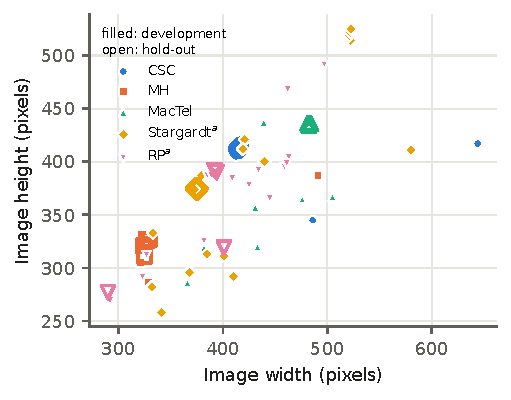
\includegraphics[width=\columnwidth]{figures/fig3_image_sizes.pdf}
\caption{Width and height of the 146 benchmark rare images, from the input lock. Filled: the 124 development images; open: the 22 hold-out images, drawn larger so that they stay visible; images of identical size overlap. Image size differs by class. The size-only reference uses only these two numbers; no model is involved. \fnRS The folder labels for RP and Stargardt disagree with the counts in the original paper.}
\label{fig:sizes}
% src: LOCK image_inventory.csv columns label, split, width, height (146 rare rows; train 124, test 22)
\end{figure}

\subsection{Post hoc analyses}
\label{sec:posthoc-methods}
After the locked results we ran agreed post hoc analyses (P0--P10, G1) and one reporting change (R1). P0--P9 and R1 were computed on a laptop from the locked features and outputs; P2 also applies the nine-way classifiers trained in our earlier work. P2 and P3 are analyses outside the locked study. G1 re-extracted MIRAGE and Inception-v3 features from padded images in one extra GPU session. P10 works on the image files. Their rules were committed before their numbers (16 November; P9 and P10 on 18 November); P0, P6 and P7 were first computed before the rules were timestamped and are labelled so.
% src: PR l.226-236, l.241-254, l.329-354, l.399-404; PR l.275, l.431-432; P10 commit dcbb323 (2026-11-18 03:42 +0700; label of every P10 CSV: "rule timestamped by commit dcbb323 (18 Nov 2026)"); P9 commit 39c3d73 (2026-11-18 01:42 +0700)
Beside every FRR we show the share of the same sources' disease images that the head calls any rare class (R1). Three of these analyses sit in the main text under one heading marked post hoc (Section~\ref{sec:res-posthoc}): size-right against size-wrong queries (P4) and CSC against MH on development images (P8), beside and never replacing the locked size-only reference, and a summary of the same-picture audit (P10), whose tables are in the supplement. The same heading opens with a side-by-side table of every $K$-shot disease task with benchmark supports (Table~\ref{tab:tasks}), which repeats numbers reported elsewhere and adds none. All others are in the supplement. No post hoc result replaces a locked one.
% src: PR l.256 (R1); placement PR HEAD 19 Nov "after the draft review" (2); PR l.229-232 (rule 2). P10 summary in the main text: agent default (coordinator brief, 21 Nov), Lam decides (rule 2: "Lam decides any other placement")

\textbf{Same-picture audit (P10).} Yoo et al.\ took the rare images from web searches, so one published picture, or slices of one case report, could sit on both sides of a split. The rule has three steps, run on a laptop with the raw files read-only. (1)~Provenance: the source list in the supplementary material of Yoo et al.\ gives links per disease, not per file, so no file could be mapped to a link. (2)~Screen: every pair of the 146 images, across labels (10,585 pairs), was scored on greyscale images by OpenCV SIFT keypoint matching (Lowe ratio 0.75, RANSAC homography with a 5-pixel threshold); the score is the inlier count. The cut-off is the largest score among 2,000 random pairs of a rare and a Kermany image, which come from different sources and cannot show the same picture: 18 inliers. On synthetic copies (each rare image re-cropped to 70--90\% of each side, rescaled by 0.5--1.5 and saved as JPEG quality 70), the screen reached the cut-off for 146 of 146. (3)~Review: one author, not a clinician, marked 55 items in random order, blind to label, split and score: the 35 rare pairs at or above the cut-off (they include the 30 highest-scoring pairs), 10 synthetic copies and 10 random low-score pairs as decoys, each as ``same picture'', ``same case, other slice'', ``different'' or ``unsure''. The marks were committed before the review key was joined. Sensitivity, beside the locked numbers and never replacing them: development macro recall (prototype, locked episodes, all four models, mean over $K=1$--8) recomputed without each query that shares a ``same picture'' or ``same case'' mark with a support of its episode, and again counting ``unsure'' as a match; hold-out recall recomputed without each hold-out image so marked against any development image.
% src: rule PR@fec827e l.254 (P10 row); step 1: PH P10_source_links.csv (79 links: 77 "no file named: S1 lists links per disease", 2 "dataset link") and P10_screen_summary.csv line 12 ("pairs sharing a source link: 0 (S1 names no file)"); step 2: P10_screen_summary.csv lines 2-5, 8-9 (10585; 2000; cut-off 18; synthetic 146, recall 1.000) and P10_screen_synthetic.csv (146 of 146 at_or_above_cutoff = 1); ratio 0.75, RANSAC 5.0 px: fm_posthoc.py l.1235 (P10_RATIO, P10_RANSAC_PX); step 3: P10_screen_summary.csv lines 6-7, 13 (35; 35; 55 items), P10_review_key.csv kinds (pair 35, of which 30 "top 30"; synthetic 10; decoy 10); marks committed abb1770 before the join (PR@fec827e l.485-486); sensitivity rule PR@fec827e l.254

\subsection{Phase-1 controls (E1--E4)}
\label{sec:phase1}
After the locked and post hoc results, internal review asked for three further checks: control image size and framing and see whether MIRAGE keeps its advantage; analyse the errors on OCTID and OCTDL, especially normal scans called another class; and test how far MIRAGE and RETFound depend on preprocessing. We turned these into four controls, E1--E4, and committed their rules on 20 November 2026, before any E number. The rules were written knowing every locked result and the post hoc results then available; two cells were known in advance (E3's padded MIRAGE is G1, and the locked values beside every E number are those of R2). Every E output is labelled post hoc and outside the locked protocol, never replaces a locked result, and is released, including failed checks. E1--E4 reuse the locked inventories, development and reporting episodes, nine-way roster and cosine prototypes; E1 and E3 draw no random numbers, and E2 and E4 use fixed seeded streams. Because the episodes are the locked ones, the same-picture pairs found by P10 sit inside them; E1 is read beside the P10 sensitivity. After the E1 verdict, one further rule (E1-D, committed 21 November 2026 before its numbers) applied P10's sensitivity unchanged to the E1-M features of MIRAGE and Inception-v3; it is descriptive and cannot change the verdict. Each new feature set has a GPU check: unchanged originals passed through the locked extraction must match the locked features (largest difference at most $10^{-4}$ of the largest absolute output; all 5,927 images for DINOv2; for MIRAGE and RETFound the first 20 per feature set, and all 5,927 through the E3 replay of the locked recipe in the first GPU session; the first 20 for Inception-v3). A model that fails is reported as ``environment differs from the lock; not interpreted''.
% src: mentor's second feedback PR@fec827e l.460-466 (M1-M3); Lam's plan l.467-476; rules added and pushed before any E number l.477-484 and l.516-521 (rule 1; commit 4b4e883, 2026-11-20 22:10 +0700); rule 2 l.522-525; rule 3 l.526-530 (two cells known); rule 4 l.531-536 (same machinery; namespaces 12101-12103, 14101-14103); duplicates inside the episodes l.496-498; Colab checks l.578-583 (tolerance 1e-4, A2 A-6); 20-image per-set controls for MIRAGE and RETFound with the 5,927-image E3 replay: PH E1a_checks.csv (control rows, "20 images"; "E3-ref full control", 5927 images) and PR@77d16a4 "Phase-1 verdicts" (disclosures). E1-D: rule commit b6d3f26 (PR change log "21 Nov, rule E1-D"), code 5e52ac6, result 4c1b79c. "internal review" = the mentor (wording: agent default, Lam decides)

\textbf{E1, size and framing control (all four models).} The main control, E1-M, renders each image once for all models: decode to RGB, which drops alpha as every locked recipe does; crop to the content box, found by applying the A2 border rule (complete edge rows, then columns, whose grey range is at most 8) again inside the remaining box until it removes nothing (a box with a side under 32\,px keeps the full frame and is counted); take the centred square of side $\min(w,h)$; resize to $256\times256$ with bicubic interpolation; save as an 8-bit RGB PNG. Each model reads that file with its own locked transform and weights. Two secondary variants are descriptive only: E1-L, a resolution floor ($128\times128$ box filter before the $256\times256$ resize), and E1-C, which only crops to the content box and leaves each model to squash or crop as locked. Three references use no model, on the same episodes and roster: the locked size-only rule, the same rule on the content box's width and height (content-size), and a $16\times16$ grey thumbnail of each input with a nearest-mean rule. A matched subset keeps the development queries whose content short side lies between the largest class minimum and the smallest class maximum; supports are not matched. \emph{Success rule} (fixed on 20 November 2026): $d_r$ is the mean over $K=1$, 2, 4 and 8 of MIRAGE E1-M minus Inception-v3 E1-M development macro recall on draw $r$; $n$ must be 100, otherwise the result is ``not evaluable''; $p_{05}$ is the 5th percentile of $d$ with linear interpolation (\texttt{numpy.percentile(d, 5)}), so the rule passes when at most four draws are non-positive and fails when six or more are. If $p_{05}>0$, MIRAGE keeps its development advantage under the size and framing control; otherwise it does not. If either model fails its control, the result is ``not evaluable'' and is never re-specified. The verdict comes from E1-M alone; E1-L, E1-C, the references, E3 and E4 are printed beside it with sentences fixed in advance and cannot overturn or rescue it. The hold-out is read for direction only, and $K=16$ is shown but not read. E1-M does not remove effective resolution, field of view, scanner appearance, compression, intensity, black-clipped background against speckle, or Kermany's white fill wedges; its centre square drops lateral retina unequally by source and class; and MIRAGE now receives 256 pixels of detail enlarged to 512.
% src: PR@fec827e l.587 (E1 row: E1-M, E1-L, E1-C, references, matched subset, success rule, fixed sentences, limitations); "passes when at most four draws are non-positive and fails when six or more": the 21 Nov correction note in the PR section 8 change log (6e4175d), which replaces the row's aside; E0 decoding and content box l.554-562; rule 5 (one verdict) l.537-538; hold-out reading l.569-572

\textbf{E2, external error analysis.} On the locked nine-way outputs and those of the E1 feature sets, a normal scan given any class but NORMAL is a \emph{failure}, and one given a rare class a \emph{false rare}; both are reported, with failures split into common disease and rare. E2 reports where OCTID (206) and OCTDL (332, from 110 patients) normal scans go, with the 169 patient-disjoint Kermany normals as calibration rows; how far the four models fail the same scans (scans failed by 0--4 models, and Jaccard indices per pair of models); how each scan's call moves from the locked to the E1-M features; and seven properties of the original files (width, height, aspect ratio, border share, near-white share, grey mean and SD) for failed and not-failed scans, as medians, failure share by tertile and an AUROC with a 95\% interval from 2,000 resamples of units (images for OCTID, patients for OCTDL). It also summarises OCTDL per patient. The rule also planned a blinded contact sheet of scans that most models fail or pass, marked by one author who is not a clinician (E2f); it was dropped under the protocol's drop order before any mark was made. E2 reports no test or $p$-value, quotes any association for all four models, and assigns no cause; it does not judge the datasets' labels.
% src: PR@fec827e l.588 (E2 row: sets, failure and false rare, E2a-E2f, allowed and not allowed); "most models" = non-NORMAL / NORMAL from >= 3 of 4 arms (E2f)

\textbf{E3, preprocessing sensitivity (MIRAGE and RETFound).} Starting from each model's locked recipe on the original images, each variant changes one step. MIRAGE: a centre crop instead of squashing, bicubic instead of bilinear resizing, no per-image min--max stretch, or a $256\times256$ input. RETFound: squashing to $256\times256$, black padding to a square, bilinear instead of bicubic resizing, a per-image min--max stretch, mean and SD of 0.5 instead of ImageNet's, or a 128-pixel short edge. G1's padded MIRAGE is shown beside them, labelled as known before the rule. Inception-v3 and DINOv2 keep their locked features. A replay of the locked recipe through the same mechanism must match the locked features within $10^{-4}$ on all 5,927 images, the crop, squash and pad variants must leave square images unchanged, and each variant must change at least one non-square image. Three criteria are fixed: (1)~for each MIRAGE variant, the 5th percentile over draws of the development $K$ mean of (variant minus locked Inception-v3) is above 0; (2)~for each RETFound variant, the 95th percentile of (variant minus locked Inception-v3) is below 0 and the 5th percentile of (locked MIRAGE minus variant) is above 0; (3)~each variant's false-rare count on OCTID and on OCTDL lies inside that model's locked 95\% interval. Scope: input preprocessing only; pooling and token choice are not varied.
% src: PR@fec827e l.589 (E3 row: base, variants, M-pad label, checks, criteria (1)-(3), scope sentence verbatim)

\textbf{E4, source separability.} E4 measures how easily the OCT sources can be told apart: Kermany (the 1,000 locked test images, patient units), the 146 benchmark images (image units, although P10 found same-picture pairs among them), OCTID (410, image units) and OCTDL (371, patient units). The main measure is a few-shot source test on the three normal-only pairs, where only the source differs (Kermany 250, OCTID 206 and OCTDL 332 normal scans): two-way cosine prototypes from $K=1$, 2, 4 and 8 units per source, every image of the other units as a query, 100 draws, two-way macro recall (chance 0.50), per model on the locked and E1-M features, with thumbnails as a pixel reference. Secondary measures are the AUROC of each geometry and grey-level column with no fit, and a logistic probe with grouped five-fold cross-validation, on the six source pairs and the three normal-only pairs; pairs with the benchmark images mix source and disease. Readings are fixed in advance: an AUROC of at least 0.95 is ``near-perfectly separable'', 0.80--0.95 ``strongly'', 0.60--0.80 ``partly'' and below 0.60 ``hardly''; when both AUROCs are at least 0.99 the pair is ``at ceiling'' and the difference is not read; ``the control reduced separability'' requires the paired interval to lie wholly below 0 (probe) or the 95th percentile of the paired $K$-mean difference to be below 0 (few-shot test). E4 does not show whether the models use the source in the rare-disease task.
% src: PR@fec827e l.590 (E4 row: sources and units, pairs, feature sets, main measure, secondary, reading, not allowed); P10 pairs: PR@fec827e l.488. Default placement (Lam decides): E1d, E1g and an E2 summary in the main text, the rest in the supplement (l.603-605); drop orders l.592-601

\section{Results}
\label{sec:results}
\subsection{Run integrity}
All four arms completed every planned episode: 2,000 prototype episodes per arm in development and 500 on the hold-out. No external image was excluded; flagged external pairs were grouped, not removed. Locked extraction times per image were 13.57\,ms (MIRAGE), 14.03\,ms (DINOv2), 23.91\,ms (RETFound) and 323.66\,ms (Inception-v3), on one NVIDIA L4 (Table~\ref{tab:pilot}).
% src: ARC runs/*/development/summary.json, runs/*/reporting/summary.json; DRV step14_external.txt lines 1-3; DRV step11_pilots.txt

\subsection{Five-way development (primary) and nomination}
MIRAGE had the highest development macro recall of the four encoders at every $K$: 0.495 at $K=1$, rising to 0.777 at $K=8$, mean 0.650 (Table~\ref{tab:dev}, Fig.~\ref{fig:recall}). DINOv2 followed (mean 0.558), then Inception-v3 (0.534) and RETFound (0.406). No other model was within 0.02 of MIRAGE, so the tie-break was not used, and MIRAGE was nominated.
% src: ARC reports/nomination/nomination.json arms.*.k_scores, .score, nominee; 0.650 - 0.558 = 0.092 > 0.02
MIRAGE minus Inception-v3 was $+0.086$, $+0.116$, $+0.132$ and $+0.130$ at $K=1$, 2, 4 and 8, and $+0.116$ on the mean over $K$ (SD 0.037; 5th--95th percentile over draws $+0.069$ to $+0.185$). The 5th percentile of the paired difference was above zero at every $K$ ($+0.001$ at $K=1$).
% src: R2 rows "MIRAGE minus Inception" (mean 0.11577, sd 0.03739, p05 0.06895, p95 0.18504; K=1 p05 0.00085); means = differences of the locked nomination.json k_scores
DINOv2 led Inception-v3 by 0.024 on the mean over $K$ ($-0.025$ to $+0.086$); the two were within 0.01 at $K=1$ and 2. RETFound was lowest at every $K$ ($-0.128$ against Inception-v3; $-0.186$ to $-0.070$).
% src: R2 rows "DINOv2 minus Inception" (0.02365; -0.0254, 0.0863; K=1 -0.0022, K=2 -0.0025) and "RETFound minus Inception" (-0.1278; -0.1864, -0.0698)
The size-only reference reached 0.578 at $K=1$ and 0.569 on the mean over $K$. At $K=1$ its mean was above every model's. MIRAGE's mean was higher from $K=2$ (0.615 against 0.550, inside the reference's 5th--95th range of 0.466--0.629 at that $K$; the comparison is of unpaired means). DINOv2 and Inception-v3 cleared it at $K=4$ and 8 only, and RETFound never did.
% src: ARC size_only_reference.csv lines 2-6; nomination.json k_scores

\begin{table*}[t]
\caption{Development five-way macro recall (primary): 124 queries, five folds pooled; mean over 100 support draws per $K$, every arm on the same supports and queries.}
\label{tab:dev}
\centering\footnotesize
\resizebox{\textwidth}{!}{% src: means ARC reports/nomination/nomination.json arms.<arm>.k_scores and .score (locked);
% src: SD and 5th-95th of arm and paired rows: PH R2_development_spread.csv (rule R2, commit 65fe98c,
%      computed 2026-11-20 after the results were known; gate: R2 means equal nomination.json within 1e-9);
%      paired means: R2 'X minus Inception' rows; size-only: ARC reports/legacy/size_only_reference.csv lines 2-6.
\begin{tabular}{@{}lccccc@{}}
\toprule
Arm & $K=1$ & $K=2$ & $K=4$ & $K=8$ & Mean $K$ 1--8 \\
\midrule
MIRAGE (nominee) & \makecell{0.495\\{\scriptsize (0.046)$^\dagger$}} & \makecell{0.615\\{\scriptsize (0.048)$^\dagger$}} & \makecell{0.712\\{\scriptsize (0.040)$^\dagger$}} & \makecell{0.777\\{\scriptsize (0.030)$^\dagger$}} & \makecell{0.650\\{\scriptsize (0.028; 0.603--0.688)$^\dagger$}} \\
DINOv2 & \makecell{0.407\\{\scriptsize (0.046)$^\dagger$}} & \makecell{0.497\\{\scriptsize (0.043)$^\dagger$}} & \makecell{0.616\\{\scriptsize (0.043)$^\dagger$}} & \makecell{0.711\\{\scriptsize (0.031)$^\dagger$}} & \makecell{0.558\\{\scriptsize (0.028; 0.511--0.606)$^\dagger$}} \\
Inception-v3 (reference) & \makecell{0.409\\{\scriptsize (0.046)$^\dagger$}} & \makecell{0.499\\{\scriptsize (0.043)$^\dagger$}} & \makecell{0.581\\{\scriptsize (0.039)$^\dagger$}} & \makecell{0.647\\{\scriptsize (0.033)$^\dagger$}} & \makecell{0.534\\{\scriptsize (0.029; 0.494--0.583)$^\dagger$}} \\
RETFound & \makecell{0.318\\{\scriptsize (0.040)$^\dagger$}} & \makecell{0.375\\{\scriptsize (0.041)$^\dagger$}} & \makecell{0.442\\{\scriptsize (0.039)$^\dagger$}} & \makecell{0.489\\{\scriptsize (0.031)$^\dagger$}} & \makecell{0.406\\{\scriptsize (0.024; 0.367--0.441)$^\dagger$}} \\
\midrule
\makecell[l]{MIRAGE $-$\\Inception-v3 (paired)} & \makecell{+0.086\\{\scriptsize (0.057; +0.001 to +0.184)$^\dagger$}} & \makecell{+0.116\\{\scriptsize (0.063; +0.015 to +0.230)$^\dagger$}} & \makecell{+0.132\\{\scriptsize (0.054; +0.052 to +0.222)$^\dagger$}} & \makecell{+0.130\\{\scriptsize (0.043; +0.071 to +0.210)$^\dagger$}} & \makecell{+0.116\\{\scriptsize (0.037; +0.069 to +0.185)$^\dagger$}} \\
\makecell[l]{DINOv2 $-$\\Inception-v3 (paired)} & \makecell{$-$0.002\\{\scriptsize (0.053; $-$0.089 to +0.077)$^\dagger$}} & \makecell{$-$0.002\\{\scriptsize (0.055; $-$0.094 to +0.087)$^\dagger$}} & \makecell{+0.036\\{\scriptsize (0.053; $-$0.046 to +0.120)$^\dagger$}} & \makecell{+0.064\\{\scriptsize (0.042; $-$0.008 to +0.136)$^\dagger$}} & \makecell{+0.024\\{\scriptsize (0.034; $-$0.025 to +0.086)$^\dagger$}} \\
\makecell[l]{RETFound $-$\\Inception-v3 (paired)} & \makecell{$-$0.090\\{\scriptsize (0.057; $-$0.182 to $-$0.000)$^\dagger$}} & \makecell{$-$0.124\\{\scriptsize (0.059; $-$0.231 to $-$0.029)$^\dagger$}} & \makecell{$-$0.139\\{\scriptsize (0.049; $-$0.217 to $-$0.060)$^\dagger$}} & \makecell{$-$0.159\\{\scriptsize (0.044; $-$0.232 to $-$0.086)$^\dagger$}} & \makecell{$-$0.128\\{\scriptsize (0.035; $-$0.186 to $-$0.070)$^\dagger$}} \\
\midrule
Size-only reference & \makecell{0.578\\{\scriptsize (0.058)}} & \makecell{0.550\\{\scriptsize (0.052)}} & \makecell{0.560\\{\scriptsize (0.051)}} & \makecell{0.589\\{\scriptsize (0.049)}} & \makecell{0.569\\{\scriptsize (0.036; 0.508--0.619)}} \\
Chance & 0.200 & 0.200 & 0.200 & 0.200 & 0.200 \\
\bottomrule
\end{tabular}
}
\par\smallskip
\parbox{\textwidth}{\footnotesize Mean $K$ 1--8 is the average over $K=1$, 2, 4, 8 that the nomination used. Cells: mean; below it, SD and 5th--95th percentiles over draws (rule R2: every $K$ and the mean over $K$). These describe variation over support draws for these images; they are not confidence intervals. Paired rows: difference from Inception-v3 on the same draws. $^\dagger$Pre-specified quantity (protocol Section~5), computed after the results were known: rule R2 committed on 19 November 2026 before computing, computed on 20 November 2026 from the locked development outputs; every mean equals the locked value. Means and the size-only row are locked. Chance is 0.20. MIRAGE was nominated; no other model was within 0.02.}
\end{table*}

\begin{figure*}[t]
\centering
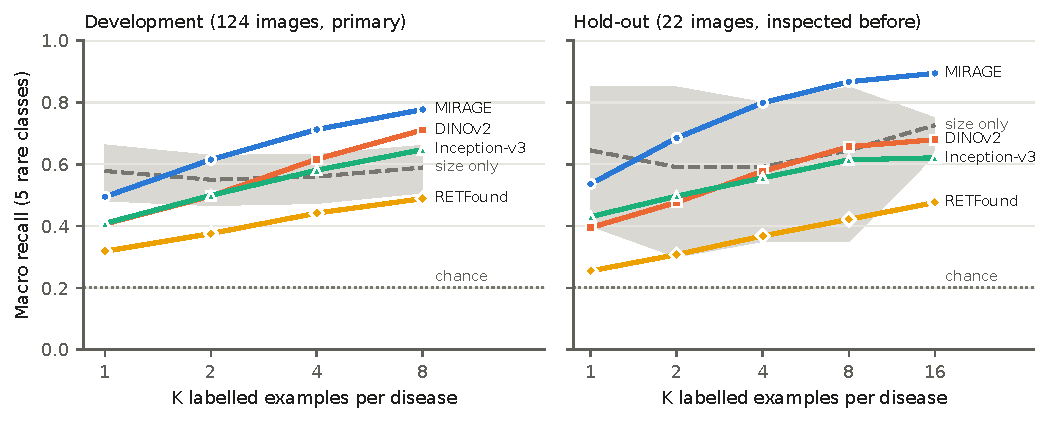
\includegraphics[width=0.92\textwidth]{figures/fig2_recall_vs_k.pdf}
\caption{Five-way macro recall against the number of labelled examples per class ($K$). Left: development, 124 queries with the five folds pooled (primary). Right: the hold-out of 22 images, a seed-42 draw matching the class counts of Yoo et al.; these images were inspected in earlier work. Lines: mean over 100 support draws per $K$; every arm sees the same supports and queries. Dashed line and grey band: size-only reference (nearest mean image width and height), mean and 5th--95th percentile over draws. Dotted line: chance (0.20). Model spreads are not drawn; development spreads are in Table~\ref{tab:dev}, hold-out spreads in Table~\ref{tab:holdout}. $K=16$ exists for the hold-out only.}
\label{fig:recall}
% src: ARC nomination.json k_scores; support_draw_summary.csv (prototype); size_only_reference.csv
\end{figure*}

\subsection{False-rare rate by source (secondary)}
\label{sec:res-frr}
MIRAGE called no patient-disjoint Kermany normal scan rare (0 of 169), 4 of 206 OCTID normal scans and 30 of 332 OCTDL normal scans (Table~\ref{tab:frr}). These rates hold for each model's locked recipe on the published, frame-filling inputs; in a post hoc preprocessing check of MIRAGE and RETFound, single changes on the same inputs moved several of their OCTID and OCTDL counts (E3, Section~\ref{sec:res-phase1}).
% src: ARC external_source_audit.csv lines 38, 52, 49; qualifier PR l.418-419; "locked recipe": PH E3_criteria.csv (3) (frame-filling one-step changes also move the counts, e.g. M-crop OCTDL 30 -> 329, M-res256 OCTID 4 -> 16; pre-freeze check 22 Nov, PR change log)
MIRAGE called only 26 of the 332 OCTDL normal scans NORMAL; it called 276 a common disease. No model called most OCTDL normal scans NORMAL: Inception-v3 called 255 of 332 a common disease, RETFound 177 and DINOv2 46, and DINOv2 instead called 141 rare (Fig.~\ref{fig:normals}). A clinic-to-clinic macular-hole analysis is in the supplement (P3, post hoc).
% src: ARC runs/<arm>/external/OCTDL/nine_way/metrics.json confusion row NORMAL (MIRAGE [26,148,118,10,...] -> 276; Inception 255; RETFound 177; DINOv2 46); external_source_audit.csv (DINOv2 OCTDL FRR 141); PR l.379-382 (pointer only, no cause)
On OCTID, all four arms called 182 to 202 of the 206 normal scans NORMAL. On all 250 Kermany normal test scans (secondary), the counts called rare were 0 (MIRAGE), 10 (DINOv2), 7 (Inception-v3) and 1 (RETFound).
% src: external_source_audit.csv recall_NORMAL numerators OCTID (189, 188, 202, 182); false_rare_rate_all lines 3, 21, 39, 57
A low FRR can also mean that the head rarely says ``rare''. On OCTID, MIRAGE called 41 of 102 CSC and 11 of 102 MH images any rare class; RETFound called none of either (R1, post hoc).
% src: PH R1_rare_beside_false_rare.csv rows MIRAGE/RETFound, OCTID
In a post hoc check that padded every image with black to a square (G1, supplement), external normal scans went almost entirely to rare classes for MIRAGE and Inception-v3 (MIRAGE called 0 of the 206 OCTID normal scans NORMAL, against 202 unpadded, and 1 of the 332 OCTDL normal scans, against 26); the false-rare rates above hold for frame-filling inputs.
% src: optional G1 sentence, one only (PR l.419-422), with the two counts the 19 Nov decision names ("MIRAGE OCTID 202 -> 0 and OCTDL 26 -> 1 called NORMAL", PR l.417), stated as observed counts with no cause (rebuttal of 23 Nov, MENTOR_LEARNING_LOG.md Feedback 3); labelled post hoc; PH G1_comparison.md section 4, rows OCTID NORMAL and OCTDL NORMAL, MIRAGE. Decided by Lam on 26 Nov (PR change log 26 Nov): one sentence with counts; the G1 table stays in the supplement

\begin{table*}[t]
\caption{Nine-way audit: truly normal scans that the head calls any of the five rare classes (count, rate and 95\% interval), with locked called-NORMAL counts and, beside them, the post hoc R1 share.}
\label{tab:frr}
\centering\footnotesize
\resizebox{\textwidth}{!}{% src: ARC reports/external/external_source_audit.csv (numerator, value, interval_low, interval_high);
%      Kermany 169 = false_rare_rate_patient_disjoint, Kermany 250 = false_rare_rate_all, OCTID/OCTDL = false_rare_rate;
%      called NORMAL = recall_NORMAL numerators; R1 (post hoc) = PH R1_rare_beside_false_rare.csv rare_called_any_rare.
\begin{tabular}{@{}lcccccc@{}}
\toprule
 & \multicolumn{4}{c}{Normal scans called any rare class: count (rate; 95\% interval)} & Called NORMAL & R1$^\ddagger$: disease images called any rare \\
\cmidrule(lr){2-5}
Arm & \makecell{Kermany, of 169\\(headline)} & \makecell{Kermany, of 250\\(secondary)} & OCTID, of 206 & OCTDL, of 332 & OCTID / OCTDL & \makecell{OCTID CSC / MH (of 102);\\OCTDL MH (of 39)} \\
\midrule
MIRAGE & \makecell{0\\{\scriptsize (0.000; 0.000--0.000)}} & \makecell{0\\{\scriptsize (0.000; 0.000--0.000)}} & \makecell{4\\{\scriptsize (0.019; 0.005--0.049)}} & \makecell{30\\{\scriptsize (0.090; 0.055--0.136)}} & 202 / 26 & 41 / 11; 3 \\
DINOv2 & \makecell{6\\{\scriptsize (0.036; 0.012--0.065)}} & \makecell{10\\{\scriptsize (0.040; 0.017--0.066)}} & \makecell{17\\{\scriptsize (0.083; 0.049--0.129)}} & \makecell{141\\{\scriptsize (0.425; 0.372--0.472)}} & 188 / 145 & 69 / 85; 39 \\
Inception-v3 & \makecell{4\\{\scriptsize (0.024; 0.006--0.049)}} & \makecell{7\\{\scriptsize (0.028; 0.008--0.053)}} & \makecell{15\\{\scriptsize (0.073; 0.041--0.117)}} & \makecell{11\\{\scriptsize (0.033; 0.012--0.059)}} & 182 / 66 & 46 / 44; 1 \\
RETFound & \makecell{1\\{\scriptsize (0.006; 0.000--0.019)}} & \makecell{1\\{\scriptsize (0.004; 0.000--0.013)}} & \makecell{0\\{\scriptsize (0.000; 0.000--0.018)}} & \makecell{18\\{\scriptsize (0.054; 0.029--0.087)}} & 189 / 137 & 0 / 0; 3 \\
\bottomrule
\end{tabular}
}
\par\smallskip
\parbox{\textwidth}{\footnotesize Kermany headline: the 169 normal test images whose patients are in no fitting row; all 250 is secondary. Intervals: 5,000 cluster resamples (seed 0), by patient for Kermany and by dependence group (each patient's images and any linked pairs) for OCTDL; exact Clopper--Pearson, image-level and conditional, for OCTID, which has no patient IDs. A zero count gets a zero-width resampling interval (MIRAGE, Kermany); zero is not shown to be the true rate, and exact bounds are in the supplement (P1, post hoc). Called NORMAL: locked counts, no interval (intervals in Table~\ref{tab:perclass}). $^\ddagger$Post hoc (R1; rule committed 16 November 2026): images that OCTID or OCTDL label CSC/CSR or MH (OCTID CSC and MH: common classes in OCTID, tier D; OCTDL MH: tier B) and that the same head calls any rare class. It shows whether a low false-rare rate comes from a head that rarely says ``rare''. These are the datasets' published labels, not clinically confirmed. The rates hold for each model's locked recipe on the published, frame-filling inputs.}
\end{table*}

\begin{figure*}[t]
\centering
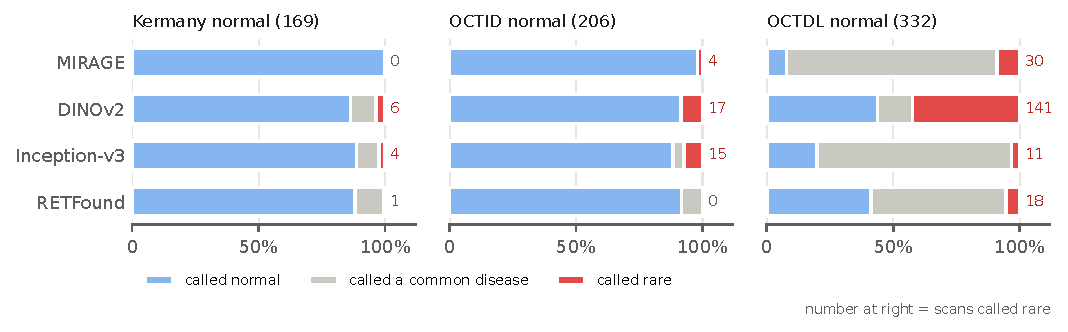
\includegraphics[width=0.92\textwidth]{figures/fig4_normal_scans.pdf}
\caption{Where truly normal scans go in the nine-way audit, by source and encoder: called NORMAL, called a common disease (CNV, DME or drusen), or called one of the five rare classes. Kermany: the 169 official normal test images whose patients are in no fitting row, the set A2 A-5 fixes for any comparison with external false-rare rates (all 250: text above). OCTID: 206 scans. OCTDL: 332 scans from 110 patients. Number at right: scans called rare. A low count can also mean that the head rarely says ``rare'': the share of the same sources' disease images it calls rare (R1) is beside each rate in Table~\ref{tab:frr}. The head has one prototype per class, from 1,000 Kermany images per common class and the 124 development rare images; no OCTID or OCTDL image is used for fitting.}
\label{fig:normals}
% src: Kermany: ARC runs/<arm>/reporting/nine_way/predictions.csv on the 169 patient-disjoint normals of LOCK nine_way_roster.csv (pid in no common fitting row), gated against runs/<arm>/reporting/nine_way/source_audit.json patient_disjoint (normal_n 169, false_rare_n); counts 169/0/0, 146/17/6, 150/15/4, 149/19/1 (NORMAL/common/rare; MIRAGE, DINOv2, Inception-v3, RETFound), equal to E2a's locked rows; OCTID, OCTDL: runs/<arm>/external/{OCTID,OCTDL}/nine_way/metrics.json, NORMAL row cells. Redrawn 26 Nov on the 169 (pre-freeze check; A2 A-5)
\end{figure*}

\subsection{Hold-out of 22 (secondary, inspected before)}
With all 124 development images as prototypes (the nine-way head), MIRAGE named 20 of the 22 hold-out images correctly, DINOv2 15, Inception-v3 13 and RETFound 9 (Table~\ref{tab:holdout}).
% src: ARC external_source_audit.csv Kermany recall_<rare class> numerators; WR l.288-291
On the five-way task, MIRAGE's macro recall was 0.722 on the mean over $K$ (SD 0.063; 5th--95th 0.615--0.830), against 0.524 for Inception-v3 and 0.618 for the size-only reference. MIRAGE minus Inception-v3 was $+0.197$ on the mean over $K$ (SD 0.085; 5th--95th $+0.042$ to $+0.343$); per $K$ it was $+0.106$ ($-0.121$ to $+0.350$) at $K=1$, $+0.188$ ($-0.020$ to $+0.440$) at $K=2$, $+0.243$ ($+0.030$ to $+0.440$) at $K=4$, $+0.253$ ($+0.060$ to $+0.390$) at $K=8$ and $+0.273$ ($+0.189$ to $+0.342$) at $K=16$.
% src: ARC support_draw_summary.csv (prototype, mean_k1_2_4_8: MIRAGE line 31, Inception line 43); size_only_reference.csv line 12; paired_differences.csv lines 62-67 (K=16 p05 0.1885 -> 0.189)
DINOv2 was level with Inception-v3 ($+0.002$; $-0.136$ to $+0.124$), and RETFound was below it ($-0.186$; $-0.308$ to $-0.052$). Against the size-only reference, MIRAGE was higher from $K=2$ on; DINOv2 was higher only at $K=8$; Inception-v3 and RETFound were never higher. At $K=16$ the size-only reference reached 0.727, above every arm except MIRAGE (0.894). With four or five images per class, these numbers show direction only.
% src: paired_differences.csv lines 55, 31; support_draw_summary.csv; size_only_reference.csv line 11 (0.7265 -> 0.727); HP D(1)

\begin{table*}[t]
\caption{Hold-out of 22 images (5 CSC, 5 MH, 4 MacTel, 4 Stargardt, 4 RP): locked nine-way exact counts per class and arm, with five-way macro recall per $K$ beside them.}
\label{tab:holdout}
\centering\footnotesize
\setlength{\tabcolsep}{3pt}
\resizebox{\textwidth}{!}{% src: nine-way counts ARC reports/external/external_source_audit.csv rows <arm>,Kermany,recall_<rare class> (numerator);
%      total = sum of the five numerators (also WR l.288-291: 20, 15, 13, 9);
%      five-way: ARC reports/legacy/support_draw_summary.csv (classifier=prototype); paired: ARC reports/legacy/paired_differences.csv
%      (MIRAGE-Inception role primary; DINOv2-, RETFound-Inception role secondary); size-only: size_only_reference.csv lines 7-12.
\begin{tabular}{@{}l*{6}{c}*{6}{c}@{}}
\toprule
 & \multicolumn{6}{c}{\makecell{Nine-way head: images named\\correctly (exact counts)}} & \multicolumn{6}{c}{Five-way prototype: macro recall, mean of 100 draws} \\
\cmidrule(lr){2-7}\cmidrule(l){8-13}
Arm & \makecell{CSC\\(5)} & \makecell{MH\\(5)} & \makecell{MacTel\\(4)} & \makecell{Starg.\textsuperscript{a}\\(4)} & \makecell{RP\textsuperscript{a}\\(4)} & \makecell{Total\\(22)} & $K=1$ & $K=2$ & $K=4$ & $K=8$ & $K=16$ & Mean $K$ 1--8 \\
\midrule
MIRAGE (nominee) & 5 & 5 & 2 & 4 & 4 & 20 & 0.536 & 0.685 & 0.799 & 0.867 & 0.894 & \makecell{0.722\\{\scriptsize (0.063; 0.615--0.830)}} \\
DINOv2 & 4 & 4 & 4 & 2 & 1 & 15 & 0.395 & 0.477 & 0.577 & 0.657 & 0.680 & \makecell{0.526\\{\scriptsize (0.065; 0.410--0.638)}} \\
Inception-v3 (reference) & 4 & 4 & 1 & 3 & 1 & 13 & 0.430 & 0.497 & 0.556 & 0.614 & 0.621 & \makecell{0.524\\{\scriptsize (0.067; 0.427--0.628)}} \\
RETFound & 1 & 1 & 2 & 1 & 4 & 9 & 0.255 & 0.308 & 0.368 & 0.422 & 0.476 & \makecell{0.338\\{\scriptsize (0.065; 0.225--0.420)}} \\
\midrule
\makecell[l]{MIRAGE $-$\\Inception-v3 (paired)} & \multicolumn{6}{c}{} & \makecell{+0.106\\{\scriptsize ($-$0.121 to +0.350)}} & \makecell{+0.188\\{\scriptsize ($-$0.020 to +0.440)}} & \makecell{+0.243\\{\scriptsize (+0.030 to +0.440)}} & \makecell{+0.253\\{\scriptsize (+0.060 to +0.390)}} & \makecell{+0.273\\{\scriptsize (+0.189 to +0.342)}} & \makecell{+0.197\\{\scriptsize (0.085; +0.042 to +0.343)}} \\
\makecell[l]{DINOv2 $-$\\Inception-v3 (paired)} & \multicolumn{6}{c}{} & \makecell{$-$0.035\\{\scriptsize ($-$0.242 to +0.200)}} & \makecell{$-$0.020\\{\scriptsize ($-$0.232 to +0.151)}} & \makecell{+0.022\\{\scriptsize ($-$0.212 to +0.191)}} & \makecell{+0.043\\{\scriptsize ($-$0.121 to +0.201)}} & \makecell{+0.059\\{\scriptsize ($-$0.070 to +0.191)}} & \makecell{+0.002\\{\scriptsize (0.083; $-$0.136 to +0.124)}} \\
\makecell[l]{RETFound $-$\\Inception-v3 (paired)} & \multicolumn{6}{c}{} & \makecell{$-$0.175\\{\scriptsize ($-$0.411 to +0.050)}} & \makecell{$-$0.189\\{\scriptsize ($-$0.401 to +0.020)}} & \makecell{$-$0.188\\{\scriptsize ($-$0.401 to +0.030)}} & \makecell{$-$0.193\\{\scriptsize ($-$0.371 to $-$0.020)}} & \makecell{$-$0.144\\{\scriptsize ($-$0.320 to 0.000)}} & \makecell{$-$0.186\\{\scriptsize (0.083; $-$0.308 to $-$0.052)}} \\
\midrule
Size-only reference & \multicolumn{6}{c}{} & 0.645 & 0.590 & 0.592 & 0.645 & 0.727 & \makecell{0.618\\{\scriptsize (0.101; 0.424--0.751)}} \\
\bottomrule
\end{tabular}
}
\par\smallskip
\parbox{\textwidth}{\footnotesize The images are a seed-42 draw from the public release that matches the class counts of Yoo et al.; they were inspected in earlier work, so the test is not blind. Nine-way head: one prototype per class, from 1,000 Kermany images per common class and all 124 development rare images; an image counts as correct only if it receives its own rare class among the nine. Five-way: $K$ supports per class from the 124 development images, 100 draws per $K$, prototype classifier; below each mean, SD and 5th--95th percentiles over draws. Paired rows: difference from Inception-v3 on the same draws. The size-only rule, in the same nine-way setting, names 17 of the 22 (post hoc, E1 reference row; Table~\ref{tab:e1g}). With 4 or 5 images per class, read for direction only. \fnRS The folder labels for RP and Stargardt disagree with the counts in the original paper; macro recall is unaffected.}
\end{table*}

\subsection{OCTID two-way test (exploratory)}
\label{sec:res-octid}
On OCTID, CSC against MH, MIRAGE's two-class macro recall was 0.737 on the mean over $K$ (SD 0.069; 5th--95th 0.613--0.842), from 0.647 at $K=1$ to 0.837 at $K=8$ (Table~\ref{tab:octid}). DINOv2 reached 0.768, Inception-v3 0.711 and RETFound 0.512. DINOv2 was higher than the nominee at $K=1$ to 8; MIRAGE was higher only at $K=16$ (0.898 against 0.863).
% src: ARC external_two_way.csv lines 2-25 (MIRAGE 14-19; DINOv2 8-13; Inception 20-25; RETFound 2-7)
MIRAGE minus Inception-v3 was $+0.026$ on the mean over $K$. The locked files hold no paired spread for this difference, and the two arms' 5th--95th ranges overlap (0.613--0.842 and 0.614--0.792). At $K=8$, MIRAGE recalled 0.849 of CSC and 0.825 of MH queries. RETFound collapsed to one class in 60, 56, 50 and 44 of 100 draws at $K=1$, 2, 4 and 8, and MIRAGE in 3 draws at $K=1$.
% src: external_two_way.csv lines 19, 25 (0.7369 - 0.7107); external_paired_differences.csv holds no two-way rows; line 17 (recall_CSC_mean, recall_MH_mean); collapsed_draws lines 2-5, 14
The size-only reference sent all 204 queries to CSC in every draw and scored 0.50. Every OCTID image is larger than every benchmark CSC and MH development image, so the reference cannot separate the two classes here. This does not test whether size differs by class inside OCTID (some CSC files are $879\times586$; every MH file is $750\times500$), and freedom from acquisition shortcuts was not established. These results measure agreement with OCTID's published labels, not clinically confirmed transfer.
% src: external_two_way.csv lines 26-31; ARC geometry_summary.csv (MIRAGE) lines 12-13, 15, 17; AM l.41, l.48-50, l.110-111; PR l.83-84

\begin{table*}[t]
\caption{OCTID central serous chorioretinopathy (OCTID ``CSR'') against macular hole, two-way (exploratory): 102 + 102 queries; macro recall over the two classes, mean of 100 draws.}
\label{tab:octid}
\centering\footnotesize
% src: ARC reports/external/external_two_way.csv columns macro_mean (per k), macro_sd/p05/p95 (mean_k1_2_4_8 line),
%      collapsed_draws (k = 1, 2, 4, 8). MIRAGE K=4 stored 0.7725 -> 0.773 under the rounding rule.
\begin{tabular}{@{}lccccccc@{}}
\toprule
Arm & $K=1$ & $K=2$ & $K=4$ & $K=8$ & $K=16$ & \makecell{Mean $K$ 1--8\\(SD; 5th--95th)} & \makecell{Draws collapsed\\($K$ = 1, 2, 4, 8)} \\
\midrule
MIRAGE (headline) & 0.647 & 0.690 & 0.773 & 0.837 & 0.898 & 0.737 (0.069; 0.613--0.842) & 3, 0, 0, 0 \\
DINOv2 & 0.669 & 0.755 & 0.805 & 0.844 & 0.863 & 0.768 (0.058; 0.665--0.848) & 0, 0, 0, 0 \\
Inception-v3 & 0.623 & 0.676 & 0.742 & 0.802 & 0.844 & 0.711 (0.051; 0.614--0.792) & 0, 0, 0, 0 \\
RETFound & 0.507 & 0.514 & 0.510 & 0.518 & 0.541 & 0.512 (0.027; 0.480--0.561) & 60, 56, 50, 44 \\
Size-only reference & 0.500 & 0.500 & 0.500 & 0.500 & 0.500 & 0.500 (0.000; 0.500--0.500) & 100, 100, 100, 100 \\
\bottomrule
\end{tabular}

\par\smallskip
\parbox{\textwidth}{\footnotesize Supports: the CSC and MH images of the locked hold-out episodes, benchmark images only. Chance is 0.50. Last column: draws in which every query went to one class. The size-only reference sent every query to CSC in every draw: every OCTID image is larger than every benchmark CSC and MH development image, so it cannot separate the two classes here; this does not test whether size differs by class inside OCTID. We evaluated agreement with OCTID's published labels; clinical label equivalence, patient independence and freedom from acquisition shortcuts were not established. Per-class recall and confusion counts: Table~\ref{tab:twoway}.}
\end{table*}

\subsection{Post hoc analyses (labelled; rules committed 16, 18, 20 and 21 November 2026)}
\label{sec:res-posthoc}
\emph{This subsection is post hoc. The rules of P4 and P8 were committed (commit 1eb3964) before their numbers were computed on 16 November 2026; the rule of P10 was committed on 18 November 2026 (commit dcbb323), and its numbers were computed on 19 and 21 November 2026. The side-by-side summary (Table~\ref{tab:tasks}) adds no number. No result here replaces a locked result.}
% src: PH P4_size_right_vs_wrong.csv and P8_csc_vs_mh_development.csv column posthoc ("post hoc, rule timestamped by commit 1eb3964 (16 Nov 2026), computed 2026-11-16"); placement PR HEAD 19 Nov "after the draft review" (2); P10: PH P10_screen_summary.csv column posthoc ("... dcbb323 (18 Nov 2026), computed 2026-11-19") and P10_sensitivity.csv ("... computed 2026-11-21; marks SHA256 15a9606fce87")

\textbf{All tasks side by side (Table~\ref{tab:tasks}).} Table~\ref{tab:tasks} sets beside each other every $K$-shot disease task with benchmark supports on which all four encoders were scored, on the mean over $K$, with the locked inputs and, where it exists, the main control E1-M. No model has the highest mean in every row. Among the locked rows, MIRAGE has it on both five-way tasks, and DINOv2 on both CSC-against-MH tasks (0.864 on development, 0.768 on OCTID). The size-only reference, which sees no pixel, is above three of the four models in both locked five-way rows and above all four on development CSC against MH (0.968); on OCTID it is at chance. Two other tasks scored all four encoders and are not rows: P3 (supplement), where OCTID or OCTDL macular holes are the examples, outside the locked study, and in which DINOv2 has the highest mean in both directions and MIRAGE the third; and E4a, a test of source, not disease (Section~\ref{sec:phase1}). The table describes the rows on file. It is not a new ranking, and each row keeps the status its rule gave it.
% src: tables/e1_tasks_summary.tex (generated; no new number): PH E1b_development.csv and E1f_holdout.csv K means (locked: MIRAGE 0.650/0.722, DINOv2 0.558/0.526, Inception 0.534/0.524, RETFound 0.406/0.338; size_only raw 0.569/0.618), P8_csc_vs_mh_development.csv mean line (0.711, 0.864, 0.794, 0.634; size_only 0.968; locked OCTID 0.737, 0.768, 0.711, 0.512), ARC external_two_way.csv size_only_reference 0.500; "no new ranking": E1 rule, "Not allowed" (PR Phase-1 controls table, E1 row); table asked for by the pre-freeze check (PR change log 22 Nov, "one locked-against-controls summary") and the mentor's review of 23 Nov; its position (here, under the post hoc heading, S5 rule 2) is the agent's default until Lam and the mentor decide (PR change log 23 and 24 Nov)

\begin{table*}[t]
\caption{Every $K$-shot disease task with benchmark supports on which all four encoders were scored, side by side: macro recall on the mean over $K=1$, 2, 4, 8 (mean of 100 support draws), with the locked inputs and under the main control E1-M, and how each row was fixed. No new number; no row replaces a locked result.}
\label{tab:tasks}
\centering\footnotesize
\resizebox{\textwidth}{!}{% src: PH E1b_development.csv and E1f_holdout.csv, k = mean_k1_2_4_8 (feature sets locked and E1-M; references
%      size_only raw, content_size raw content box, thumbnail raw and E1-M); the locked development cells equal
%      R2_development_spread.csv (checked);
%      PH P8_csc_vs_mh_development.csv mean line (mean; locked_OCTID_two_way_macro_mean = Table 4);
%      OCTID size-only 0.500: ARC reports/external/external_two_way.csv size_only_reference (Table 4); typed here,
%      as in t6, because P8's CSV leaves that cell empty. Hold-out and OCTID locked cells are copies held by the
%      E1f and P8 files; they were compared with the archive on 24 Nov 2026 (equal).
%      Generated by make_tables.py; formatting only, no new number.
\begin{tabular}{@{}lllcccccccc@{}}
\toprule
Task & Inputs & How the row was fixed & MIRAGE & DINOv2 & Inception-v3 & RETFound & Size-only & Content-size$^{\dagger}$ & Thumbnail$^{*}$ & Chance \\
\midrule
Development, five-way (124 queries) & locked & registered (primary) & 0.650 & 0.558 & 0.534 & 0.406 & 0.569 & 0.447 & 0.288 & 0.20 \\
 & E1-M & post hoc, E1 (rule 20 Nov) & 0.649 & 0.542 & 0.586 & 0.412 & -- & 0.447 & 0.360 & 0.20 \\
\addlinespace[2pt]
Hold-out, five-way (22 queries) & locked & registered (secondary; not blind) & 0.722 & 0.526 & 0.524 & 0.338 & 0.618 & 0.455 & 0.237 & 0.20 \\
 & E1-M & post hoc, E1 (rule 20 Nov) & 0.667 & 0.553 & 0.571 & 0.341 & -- & 0.455 & 0.275 & 0.20 \\
\addlinespace[2pt]
Development, CSC against MH & locked & post hoc, P8 (rule 16 Nov) & 0.711 & 0.864 & 0.794 & 0.634 & 0.968 & -- & -- & 0.50 \\
OCTID, CSC against MH & locked & registered (exploratory) & 0.737 & 0.768 & 0.711 & 0.512 & 0.500 & -- & -- & 0.50 \\
\bottomrule
\end{tabular}
}
\par\smallskip
\parbox{\textwidth}{\footnotesize Registered rows repeat the locked results (Tables~\ref{tab:dev}, \ref{tab:holdout} and~\ref{tab:octid}); post hoc rows repeat Tables~\ref{tab:p8} and~\ref{tab:e1d} and the supplement (E1b, E1f), each under the rule and date shown. E1-M: every image cropped to its content, squared and resized once for all models (Section~\ref{sec:phase1}); the two-way tasks were not scored under it. Size-only: nearest mean width and height of the original file; under E1-M every input is a 256-pixel square, so the file size no longer reaches the model. $^{\dagger}$Content-size: the same rule on the width and height of each image's content box (bands removed); E1-M squares that box on its short side, so the short side still reaches the model as effective resolution; a post hoc reference (E1), the same in the locked and E1-M rows. Not in the table: P3 (supplement, outside the locked study) and E4a (source, not disease). $^{*}$Thumbnail: a $16\times16$ grey copy of each input with a nearest-mean rule; a post hoc reference (E1) in every row, not computed for the two-way tasks. Spreads over draws are in the tables named; the hold-out has four or five images per class and shows direction only. The external false-rare counts, locked and under the control, are in Table~\ref{tab:e1g}.}
\end{table*}

\textbf{Size-right against size-wrong queries (P4).} In the locked development episodes, the size-only rule named 0.594 of query cells correctly (29,441 of 49,600). Table~\ref{tab:p4} splits each episode's queries by whether the size-only rule named them correctly and gives each model's recall in each group. Every model scored higher on size-right than on size-wrong queries on the mean over $K$: MIRAGE 0.663 against 0.646, DINOv2 0.577 against 0.537, Inception-v3 0.543 against 0.509 and RETFound 0.443 against 0.394. For MIRAGE the order reversed at $K=4$ (0.708 against 0.730) and $K=8$ (0.762 against 0.795). This is a description, not proof that any model uses image size.
% src: PH P4_size_right_vs_wrong.csv line 42 (share_of_query_cells_size_right 0.59357, 29441/49600); mean_k1_2_4_8 rows (MIRAGE 0.66279/0.64587; DINOv2 0.57694/0.53742; Inception 0.54295/0.50910; RETFound 0.44334/0.39361); MIRAGE K=4 0.70769/0.73035, K=8 0.76224/0.79496; PR l.247 ("A description, not proof")

\textbf{CSC against MH on development (P8).} P8 is the like-for-like comparator for the OCTID two-way test: development CSC and MH queries only, with the same two-way rule (Table~\ref{tab:p8}). On the mean over $K$, DINOv2 scored 0.864, Inception-v3 0.794, MIRAGE 0.711 and RETFound 0.634, and the size-only rule scored 0.968, above every model. MIRAGE minus Inception-v3 was $-0.083$ (SD 0.052; 5th--95th $-0.164$ to $+0.010$), against $+0.026$ on OCTID.
% src: PH P8_csc_vs_mh_development.csv lines 11, 16, 21, 6, 26, 31 (0.8639, 0.7106, 0.7940, 0.6343; size_only 0.9680; MIRAGE-Inception -0.0834, sd 0.0524, p05 -0.1636, p95 +0.0104; locked column 0.0261); PR l.251

\textbf{Provenance of the release and same-picture audit (P10).} The public release is not the set described in the original paper. Version 1 holds 119 images, the total in Yoo et al.; version 2, which we use, holds 146, and its folders hold RP 31 and Stargardt 23 images where the paper gives Stargardt 19 and RP 16 (Section~\ref{sec:methods}; a file-identity check, made outside any rule and labelled so in the supplement). Inside the 146 images, a keypoint screen and a blind review found 14 same-picture pairs (Table~\ref{tab:p10pairs}). One further pair was marked the same case on another slice (MacTel/09 and MacTel/23) and one unsure (CSC/26 and CSC/27, noted as probably a follow-up visit); the other 19 screened pairs were marked different. All 10 synthetic copies were marked ``same picture'' and all 10 decoys ``different''. The locked duplicate screen had flagged none of the 14 pairs. Four of the 22 hold-out images have a same-picture copy among the development images: MacTel/19, RP/17, RP/20 and Stargardt/03 (five pairs; Stargardt/03 matches two development images).
% src: provenance: PR l.59-67 and Section III-B "Provenance" (v1 119, v2 146; paper Stargardt 15+4, RP 12+4; v2 folders RP 31, Stargardt 23), pre_rule/2026-11-18/v1_to_ours.csv (pre-rule label); joined with P10 in one paragraph after the mentor's review of 23 Nov (MENTOR_LEARNING_LOG.md, "Provenance: one results subsection"); five pairs: PH P10_matched_pairs.csv lines 6, 10, 12, 13, 14 (Stargardt/03 with Stargardt/08 and Stargardt/14)
% src: PH P10_review_marks.csv joined with P10_review_key.csv on item (kind "pair": 14 "same picture", 1 "same case, other slice" = item 26 MacTel/23-MacTel/09, 1 "unsure" = item 11 CSC/26-CSC/27 with note "... probably a follow-up visit ...", 19 "different"; kind "synthetic": 10 "same picture"; kind "decoy": 10 "different"); PR@fec827e l.485-491; hold-out images: PH P10_matched_pairs.csv rows with set "hold-out" (MacTel/19, RP/20, RP/17, Stargardt/03)
Removing the matched pairs (14 same picture, 1 same case) changes the development comparison by less than 0.005. Without each development query matched to a support of its episode, MIRAGE minus Inception-v3 on the mean over $K$ moved from $+0.116$ to $+0.113$ (5th percentile over draws $+0.069$ to $+0.064$). Without the four hold-out images, MIRAGE's hold-out macro recall moved from 0.722 to 0.751, and MIRAGE minus Inception-v3 from $+0.197$ to $+0.240$. Counting the unsure pair as a match changed neither difference by more than 0.001 (Table~\ref{tab:p10}). These are sensitivity values beside the locked results; the locked values above remain the reported results.
% src: PH P10_sensitivity.csv (k = mean_k1_2_4_8): development "MIRAGE minus Inception" line 36 (locked 0.115769, p05 0.068949), line 110 (same picture or case excluded: 0.112920, p05 0.064039), line 184 (also unsure: 0.113127, p05 0.063710); hold-out MIRAGE line 54 (0.721599) and line 128 (0.751016); hold-out "MIRAGE minus Inception" line 75 (0.197375) and lines 149, 223 (0.240083); wording PR@fec827e l.495-496 ("removing them changes the development comparison by less than 0.005"; 0.115769 - 0.112920 = 0.0028)

\begin{table}[t]
\caption{Post hoc (P4; rule committed 16 Nov 2026, computed 16 Nov 2026). Development macro recall on queries the size-only rule names correctly (size-right) and wrongly (size-wrong), in the same episodes.}
\label{tab:p4}
\centering\footnotesize
\setlength{\tabcolsep}{4pt}
% src: PH P4_size_right_vs_wrong.csv column mean_episode_macro (lines 2-41); label: post hoc, rule timestamped by commit 1eb3964 (16 Nov 2026), computed 2026-11-16
\begin{tabular}{@{}llccccc@{}}
\toprule
Arm & Queries & $K=1$ & $K=2$ & $K=4$ & $K=8$ & Mean \\
\midrule
MIRAGE & size-right & 0.546 & 0.635 & 0.708 & 0.762 & 0.663 \\
 & size-wrong & 0.451 & 0.607 & 0.730 & 0.795 & 0.646 \\
\addlinespace[2pt]
DINOv2 & size-right & 0.415 & 0.518 & 0.641 & 0.735 & 0.577 \\
 & size-wrong & 0.395 & 0.476 & 0.597 & 0.682 & 0.537 \\
\addlinespace[2pt]
Inception-v3 & size-right & 0.411 & 0.509 & 0.595 & 0.656 & 0.543 \\
 & size-wrong & 0.405 & 0.483 & 0.544 & 0.605 & 0.509 \\
\addlinespace[2pt]
RETFound & size-right & 0.372 & 0.416 & 0.475 & 0.510 & 0.443 \\
 & size-wrong & 0.292 & 0.359 & 0.429 & 0.495 & 0.394 \\
\bottomrule
\end{tabular}

\par\smallskip
\parbox{\columnwidth}{\footnotesize Mean of per-episode macro recall over 500 fold-level episodes per $K$ (5 folds $\times$ 100 draws); a class with no query in a group in an episode is left out of that episode's average. Mean: average of the four $K$. How many episodes each class enters is in the supplement (P4). A description, not proof.}
\end{table}

\begin{table*}[t]
\caption{Post hoc (P8; rule committed 16 Nov 2026, computed 16 Nov 2026). CSC against MH on the development images, two-way (larger of the two cosines, ties to CSC): the like-for-like comparator for Table~\ref{tab:octid}.}
\label{tab:p8}
\centering\footnotesize
% src: PH P8_csc_vs_mh_development.csv lines 2-31 (mean; sd/p05/p95 on the mean line; paired per k p05/p95);
%      last column = locked_OCTID_two_way_macro_mean on the mean line (= Table 4). Label: post hoc, rule timestamped by commit 1eb3964 (16 Nov 2026), computed 2026-11-16
\begin{tabular}{@{}lcccccc@{}}
\toprule
Arm & $K=1$ & $K=2$ & $K=4$ & $K=8$ & \makecell{Mean $K$ 1--8\\(SD; 5th--95th)} & \makecell{OCTID\\(locked)} \\
\midrule
MIRAGE & 0.613 & 0.674 & 0.744 & 0.811 & \makecell{0.711\\{\scriptsize (0.038; 0.658--0.782)}} & 0.737 \\
DINOv2 & 0.744 & 0.845 & 0.910 & 0.957 & \makecell{0.864\\{\scriptsize (0.036; 0.807--0.921)}} & 0.768 \\
Inception-v3 & 0.681 & 0.762 & 0.836 & 0.897 & \makecell{0.794\\{\scriptsize (0.040; 0.724--0.863)}} & 0.711 \\
RETFound & 0.561 & 0.603 & 0.657 & 0.716 & \makecell{0.634\\{\scriptsize (0.039; 0.575--0.688)}} & 0.512 \\
Size-only & 0.938 & 0.973 & 0.981 & 0.981 & \makecell{0.968\\{\scriptsize (0.018; 0.934--0.981)}} & 0.500 \\
\midrule
\makecell[l]{MIRAGE $-$\\Inception-v3 (paired)} & \makecell{$-$0.068\\{\scriptsize ($-$0.174 to +0.119)}} & \makecell{$-$0.088\\{\scriptsize ($-$0.230 to +0.072)}} & \makecell{$-$0.092\\{\scriptsize ($-$0.192 to +0.019)}} & \makecell{$-$0.086\\{\scriptsize ($-$0.172 to $-$0.001)}} & \makecell{$-$0.083\\{\scriptsize (0.052; $-$0.164 to +0.010)}} & +0.026 \\
\bottomrule
\end{tabular}

\par\smallskip
\parbox{\textwidth}{\footnotesize Locked development episodes, CSC and MH queries only; mean of 100 draws; chance 0.50. Paired row: per $K$, mean (5th to 95th percentile). Last column: the locked OCTID two-way mean over $K$ (Table~\ref{tab:octid}), shown for comparison.}
\end{table*}

\subsubsection{Phase-1 controls E1--E4 (rules committed 20 November 2026)}
\label{sec:res-phase1}
\emph{This part is post hoc. Its rules were committed on 20 November 2026 (commit 4b4e883) before any E number, and the E numbers were computed once, on 21 November 2026, after both GPU sessions. Every check passed (supplement, E1a and E3): each new feature set matched the locked features through the locked path within $10^{-4}$, the replay of the locked recipe matched on all 5,927 images for MIRAGE and RETFound, and every E3 variant changed the features. A recomputation with separate code gave the same E1 and E3 values. No result here replaces a locked result.}
% src: PH E1a_checks.csv (rule 1 SHA256 "same"; 25 receipts "equal"; 12 controls "pass", max ratio 2.8e-6; E3-ref full control MIRAGE 2.99e-7, RETFound 1.91e-7, 5927 images); PH E3_checks.csv (square checks pass; ten variants "change applied"); scored once after Session 2: PR@77d16a4 change log 21 Nov ("E1-E4 scored once"; "Phase-1 verdicts": independent recompute by GPT-6.2 Sol equal to the committed values)

\textbf{E1, size and framing control (Table~\ref{tab:e1d}).} Under the size and framing control, MIRAGE keeps a positive development advantage over Inception-v3 (mean 0.063, locked 0.116; p05 0.0025), and also when effective resolution is evened out (E1-L p05 = 0.023), and also when the image is only cropped to its content box (E1-C p05 = 0.017); it is above the pixel-only reference (mean 0.290). The margin is small: the 5th percentile is 0.0025, with 95 of the 100 draws above 0, so a sixth non-positive draw would have failed the rule. The rule measures how stable the lead is over support draws on the 124 fixed development queries; it sets no minimum size for the lead, and the uncertainty of the 5th percentile itself was not estimated. MIRAGE's own development score barely moved (0.650 locked, 0.649 under E1-M), while Inception-v3 rose from 0.534 to 0.586 (E1-M minus locked $+0.052$, 5th percentile $+0.006$); Inception-v3's E1 input also reaches the model by a different path from its locked input (another decoder and another resampling step; supplement, E1a), so its rise is a response to the whole E1-M input path. The decoder check in E1a holds 40 Kermany, OCTID and OCTDL files and no rare image, and E3 gives Inception-v3 no preprocessing grid, so the step that produced the rise was not separated. The control moved the other comparisons too: DINOv2 minus Inception-v3 went from $+0.024$ locked to $-0.044$ under E1-M (95th percentile $+0.004$), and Inception-v3's mean under E1-M (0.586) was above the raw size-only mean (0.569, unpaired). Against the raw size-only reference, which reads file dimensions that the controlled squares no longer carry, only unpaired means exist: MIRAGE under E1-M was above it on the mean over $K$ (0.649 against 0.569) and below it at $K=1$ (0.486 against 0.578). The hold-out is read for direction only (the sign of the paired difference, next paragraph). Its printed levels are shown, not read: MIRAGE's own mean over $K$ was 0.722 locked and 0.667 under E1-M (unpaired means on 22 images), and the nine-way head named 18 of the 22 images correctly for MIRAGE and 16 for Inception-v3 (locked: 20 and 13). These lines describe; they make no new ranking.
% src: other arms and hold-out (pre-freeze check 22 Nov, PR change log): PH E1c_paired.csv lines 11, 26 ("DINOv2 minus Inception" locked 0.0236, E1-M -0.0442, p95 0.0044); E1b_development.csv lines 71, 86 (Inception E1-M 0.5864; size_only raw 0.5693); E1g_nine_way.csv "Legacy 22" correct_class (MIRAGE locked 20, E1-M 18; Inception locked 13, E1-M 16); decoder check holds no rare image: PR E1 row ("20 Kermany, 10 OCTID, 10 OCTDL originals") and E1a_checks.csv lines 78-80; resampling: PR E1 row (E1-M resizes with PIL BICUBIC; "stage3_classifier.load_image, whose 256 x 256 resize leaves the input unchanged"); E3 scope: MIRAGE and RETFound only (PR E3 row)
% src: PH E1d_success.csv rows locked/E1-M/E1-L/E1-C (mean 0.115770/0.063136, p05 0.068949/0.002519/0.022859/0.016706; draws above 0: 95) and companion lines (thumbnail E1-M mean 0.290, p05 0.243); fixed sentence verbatim from E1_comparison.md "Sentence"; "a sixth non-positive draw would have failed": with 95 of 100 above 0, p05 = 0.05 d(5) + 0.95 d(6) is <= 0 once d(6) <= 0 (the sixth-draw value has no file of record and was dropped, PR change log 22 Nov); E1b_development.csv K mean (MIRAGE 0.650/0.649; Inception 0.534/0.586); E1c_paired.csv "Inception E1-M minus Inception locked" (0.052, p05 0.006); E1a_checks.csv "Inception-v3 decoder change" (0.020-0.046); whole input path and "uncertainty of p05 not estimated": PR change log "22 Nov, pre-freeze double-check"; what the rule measures: PR E0 ("This spread is over support draws on 124 fixed queries, not a confidence interval"); raw size-only: PH E1b_development.csv lines 82, 86 (0.5780, 0.5693) against MIRAGE E1-M lines 47, 51 (0.4856, 0.6495), unpaired (no paired MIRAGE minus raw size-only row exists); hold-out levels: PH E1f_holdout.csv lines 100, 111 (0.7216, 0.6673)
Beside the verdict, as descriptions that cannot change it: per $K$, the 5th percentile of MIRAGE minus Inception-v3 under E1-M was $-0.068$, $-0.034$, $+0.015$ and $+0.016$ at $K=1$, 2, 4 and 8 (locked $+0.001$, $+0.015$, $+0.052$ and $+0.071$); on the 92 development queries of matched content size it had mean $+0.057$ and 5th percentile $-0.012$ (supports not matched); and on the hold-out the mean paired difference was positive at $K=1$, 2, 4 and 8 and on the mean over $K$ in all four feature sets ($+0.096$ for E1-M). The same-picture pairs found by P10 sit inside these episodes; removing them moved the locked 5th percentile from 0.069 to 0.064 (Section~\ref{sec:res-posthoc}). Under the rule added after the verdict (E1-D, post hoc, supplement): ``Without the same-picture pairs, MIRAGE's development lead over Inception-v3 under E1-M has mean 0.064 and 5th percentile 0.0062 (with them: 0.063 and 0.0025).'' As in P10, the excluded matches are the 14 same-picture pairs and one same-case pair. Counting the unsure pair as a match too, the 5th percentile was 0.0090, and on the hold-out without the four copied images the mean paired difference stayed positive ($+0.069$, direction only). The limitations listed in Section~\ref{sec:phase1} apply to every E1 result.
% src: PH E1c_paired.csv "MIRAGE minus Inception" k=1,2,4,8 (E1-M p05 -0.0677, -0.0342, 0.0146, 0.0163; locked 0.00085, 0.0151, 0.0520, 0.0713); E1e_matched.csv (92 queries, L=164, U=296; E1-M 0.057, p05 -0.012); E1f_holdout.csv direction rows (all "positive"; E1-M mean_k1_2_4_8 0.096); P10_sensitivity.csv (0.068949 -> 0.064039); E1-D: PH E1D_duplicate_sensitivity.csv (sentence row verbatim; E1-M "also counting unsure" mean_k1_2_4_8 p05 0.008961; hold-out E1-M "marked same picture or same case" mean 0.068533); rule PR section 8 change log "21 Nov, rule E1-D" (b6d3f26), code 5e52ac6

In the nine-way audit (Table~\ref{tab:e1g}), MIRAGE under E1-M called none of the 169 Kermany normals and none of the 206 OCTID normals rare (locked: 0 and 4), and 34 of 102 OCTID CSR and 13 of 102 OCTID MH images rare (R1). On OCTDL it called 261 of 332 normal scans rare (0.786; locked 30, 0.090) and all 39 MH scans rare. Under E1-M, Inception-v3 called 76 of 206 OCTID and 94 of 332 OCTDL normals rare (locked 15 and 11), RETFound 0 and 131 (locked 0 and 18), and DINOv2 2 and 80 (locked 17 and 141). The E1-M thumbnail reference called 331 of 332 OCTDL normals rare. No cause is assigned to any of these rates.
% src: PH E1g_nine_way.csv rows E1-M and locked, query sets Kermany patient-disjoint, OCTID NORMAL, OCTID CSC, OCTID MH, OCTDL NORMAL, OCTDL MH (MIRAGE E1-M 0/169, 0/206, 34/102, 13/102, 261/332 rate 0.786, 39/39; locked 0, 4, 30 rate 0.090; Inception E1-M 76, 94, locked 15, 11; RETFound E1-M 0, 131, locked 0, 18; DINOv2 E1-M 2, 80, locked 17, 141; thumbnail E1-M OCTDL 331/332); PR@fec827e l.587 (no cause)

\textbf{E2, external error analysis (Tables~\ref{tab:e2} and~\ref{tab:e2d}).} With locked features, OCTID normal scans failed in 4 to 24 of 206 per model, and none failed in three or more models. OCTDL normal scans failed in 187 to 306 of 332 per model; 98 failed in all four models and 2 in none. The locked OCTDL failures were mostly common-disease calls for MIRAGE (276 of 306), Inception-v3 (255 of 266) and RETFound (177 of 195), and mostly rare calls for DINOv2 (141 of 187). Under E1-M, OCTDL common-disease calls moved to rare classes for MIRAGE (228 of 276), RETFound (64 of 177) and Inception-v3 (72 of 255), while DINOv2 moved the other way (42 of its 141 rare calls to common disease), and Inception-v3 failed 81 of 206 OCTID normals. For the seven image properties, 45 of the 133 reported intervals exclude 0.5; the 133 include 42 Kermany calibration rows (17 of the 45) and 24 intervals that are constant at 0.5 (none of the 45). On OCTDL normals with locked features, the AUROC of grey mean for failed against not-failed scans was 0.807 for RETFound, 0.635 for MIRAGE, 0.586 for DINOv2 and 0.584 for Inception-v3. These are associations among these scans, not causes, and they say nothing about the datasets' labels. The blinded contact sheet (E2f), which sets normal scans that most models fail beside those most models pass, was not marked: it was dropped under the protocol's laptop drop order, where it comes first.
% src: PH E2a_destinations.csv locked OCTID NORMAL failures (RETFound 17, DINOv2 18, MIRAGE 4, Inception 24) and OCTDL NORMAL (RETFound 195 = 177 common + 18 rare, DINOv2 187 = 46 + 141, MIRAGE 306 = 276 + 30, Inception 266 = 255 + 11); E1-M OCTID Inception 5 + 76 = 81; E2b_overlap.csv (OCTID failed by >= 3 arms: 0; OCTDL failed by 4 arms: 98, by 0: 2); E2c_transitions.csv (MIRAGE common->rare 228; RETFound 64; Inception 72; DINOv2 rare->common 42); E2_comparison.md ("45 of 133"; OCTDL grey_mean AUROC 0.807, 0.635, 0.586, 0.584); PR@fec827e l.588 (no cause; all four arms; labels); E2f dropped: PR@00a7474 l.726 (laptop drop order, E2f first) and change log 22 Nov (Lam)

\textbf{E3, preprocessing sensitivity (supplement, E3).} Input preprocessing only; pooling and token choice are not varied. (1)~MIRAGE: kept within this grid; the 5th percentile of each variant minus locked Inception-v3 ranged from 0.043 (M-res256) to 0.075 (M-bicubic) (G1's padded MIRAGE, shown beside and not counted: 0.060). (2)~RETFound: position changed or not shown for R-norm05; the other five variants met both conditions. With mean and SD 0.5 instead of ImageNet's, RETFound's development mean over $K$ rose from 0.406 to 0.578; its difference from locked Inception-v3 had mean $+0.044$ and 95th percentile $+0.110$, and locked MIRAGE minus this variant had 5th percentile $+0.018$. (3)~External false-rare counts: not all inside; 10 of the 20 counted cells lay outside the model's locked 95\% interval, in both directions. They were above it for MIRAGE M-crop (OCTID 17 of 206, OCTDL 329 of 332) and M-res256 (OCTID 16), and RETFound R-pad (OCTID 118, OCTDL 332 of 332) and R-norm05 (OCTDL 43); below it for MIRAGE M-bicubic (OCTID 1) and M-nostretch (OCTID 0), and RETFound R-bilinear (OCTDL 5) and R-res128 (OCTDL 2). NORMAL recall and R1 for each cell are in the supplement.
% src: PH E3_criteria.csv rows (1) (p05 M-crop 0.0707, M-bicubic 0.0753, M-nostretch 0.0669, M-res256 0.0432; result "kept within this grid"; M-pad 0.0595 "shown beside, not counted"), (2) (R-norm05 p95 0.1098 "not met", MIRAGE locked - R-norm05 p05 0.0179 "met"; result "position changed or not shown for R-norm05"), (3) (ten counted cells outside; counts as quoted); E3_development.csv RETFound R-norm05 K mean 0.578, locked 0.406, and its paired row R-norm05 minus Inception-v3 locked, mean_k1_2_4_8 (mean 0.044089); scope sentence verbatim PR@fec827e l.589

\textbf{E4, source separability (supplement, E4).} In the few-shot source test on the three normal-only pairs, two-way macro recall on the mean over $K$ ranged from 0.779 to 0.996 across models, locked and E1-M (chance 0.50), and from 0.820 to 0.923 for the thumbnails. The control reduced separability for Inception-v3 (Kermany against OCTDL, and OCTID against OCTDL) and for MIRAGE (OCTID against OCTDL); no reduction was shown elsewhere. In the logistic probe, every normal-only pair was near-perfectly separable (AUROC at least 0.994) and at ceiling, so differences there are not read. E4 does not show whether the models use the source in the rare-disease task.
% src: PH E4a_fewshot_source_test.csv mean_k1_2_4_8 two-way rows (min DINOv2 locked Kermany vs OCTDL 0.7791; max MIRAGE E1-M Kermany vs OCTID 0.9964; thumbnails 0.8197-0.9230) and paired rows "the control reduced separability" (Inception Kermany vs OCTDL p95 -0.035, Inception OCTID vs OCTDL p95 -0.007, MIRAGE OCTID vs OCTDL p95 -0.005); E4c_probe_auroc.csv normal-only pairs (33 cells, min 0.9940); reading bands PR@fec827e l.590
\havetable{e1d_success}\ifgen
\begin{table*}[t]
\caption{Post hoc, Phase-1 E1 (rule committed 20 Nov 2026): size and framing control. MIRAGE minus Inception-v3, development macro recall averaged over $K=1$, 2, 4, 8 within each of the 100 paired draws, per feature set, with the companion lines.}
\label{tab:e1d}
\centering\footnotesize
% src: E1d_success.csv in results/fm_v1/posthoc (generated by make_tables.py; formatting only);
% label: post hoc, Phase-1 rule E1 timestamped by commit 4b4e883 (20 Nov 2026), computed 2026-11-21; outside the locked protocol; never replaces a locked result; limitations: the centre square drops lateral retina unequally by source and class; MIRAGE now gets 256 px of detail enlarged to 512; E1-M does not remove effective resolution (content short side 103-496 px), field of view, scanner appearance, compression, intensity, black-clipped background against speckle, or Kermany's white fill wedges
% cells: n_draws, mean, sd, p05 (four decimals), draws_above_0, verdict as stored; mean and p05 are paired differences.
\begin{tabular}{@{}p{4.4cm}lp{2.2cm}cccccl@{}}
\toprule
Line & Feature set & Status & $n$ & Mean & SD & p05 & Draws $>0$ & Verdict \\
\midrule
MIRAGE $-$ Inception-v3 & locked & interpreted & 100 & +0.116 & 0.037 & +0.0689 & 100 & description only \\
MIRAGE $-$ Inception-v3 & E1-M & interpreted & 100 & +0.063 & 0.036 & +0.0025 & 95 & pass \\
MIRAGE $-$ Inception-v3 & E1-L & interpreted & 100 & +0.077 & 0.034 & +0.0229 & 99 & description only \\
MIRAGE $-$ Inception-v3 & E1-C & interpreted & 100 & +0.068 & 0.033 & +0.0167 & 98 & description only \\
MIRAGE E1-M $-$ Content-size reference (raw content box) & E1-M & interpreted & 100 & +0.203 & -- & +0.1493 & 100 & companion line \\
MIRAGE E1-M $-$ Thumbnail reference (E1-M) & E1-M & interpreted & 100 & +0.290 & -- & +0.2427 & 100 & companion line \\
\bottomrule
\end{tabular}

\par\smallskip
\parbox{\textwidth}{\footnotesize Only the E1-M row gives the verdict ($p_{05}>0$ over the 100 paired draws); the other feature sets and the companion lines are descriptions and cannot overturn or rescue it. Spread over support draws on 124 fixed queries, not a confidence interval. Verdict on E1-M: \textbf{pass}. Fixed sentence: ``Under the size and framing control, MIRAGE keeps a positive development advantage over Inception-v3 (mean 0.063, locked 0.116; p05 0.003), and also when effective resolution is evened out (E1-L p05 = 0.023), and also when the image is only cropped to its content box (E1-C p05 = 0.017); it is above the pixel-only reference (mean 0.290).''
 Limitations stated with every E1 result: the centre square drops lateral retina unequally by source and class; MIRAGE now gets 256 px of detail enlarged to 512; E1-M does not remove effective resolution (content short side 103-496 px), field of view, scanner appearance, compression, intensity, black-clipped background against speckle, or Kermany's white fill wedges.
 (Correction: the measured content short side of the 146 rare images is 103--471\,px; the rule's text says 103--496\,px.) Label: post hoc, Phase-1 rule E1 timestamped by commit 4b4e883 (20 Nov 2026), computed 2026-11-21; outside the locked protocol; never replaces a locked result
.}
\end{table*}
\fi
\havetable{e1g_nine_way}\ifgen
\begin{table*}[t]
\caption{Post hoc, Phase-1 E1 (rule committed 20 Nov 2026): nine-way audit per model and feature set. Normal scans called any rare class (count/$n$, rate and 95\% interval by the locked method), normal scans called NORMAL or a common disease (two counts per source, in the order Kermany; OCTID; OCTDL), external disease images called any rare class (R1) and hold-out images named correctly.}
\label{tab:e1g}
\centering\footnotesize
\resizebox{\textwidth}{!}{% src: E1g_nine_way.csv in C:/Users/ThinkBook/.t3/worktrees/Few-shot/t3-03f3a2c4/results/fm_v1/posthoc (generated by make_tables.py; formatting only);
% label: post hoc, Phase-1 rule E1 timestamped by commit 4b4e883 (20 Nov 2026), computed 2026-11-21; outside the locked protocol; never replaces a locked result; limitations: the centre square drops lateral retina unequally by source and class; MIRAGE now gets 256 px of detail enlarged to 512; E1-M does not remove effective resolution (content short side 103-496 px), field of view, scanner appearance, compression, intensity, black-clipped background against speckle, or Kermany's white fill wedges
% cells: called_any_rare/n (rate_value; ci95_low--ci95_high) on the normal sets; called_NORMAL; R1 = called_any_rare
%        on OCTID CSC, OCTID MH, OCTDL MH; hold-out = correct_class of 'Legacy 22'.
\begin{tabular}{@{}llcccccc@{}}
\toprule
 & & \multicolumn{3}{c}{Normal scans called any rare class: count/$n$ (rate; 95\% interval)} & & & \\
\cmidrule(lr){3-5}
Model & Set & \makecell{Kermany normals\\(patient-disjoint)} & OCTID normals & OCTDL normals & \makecell{Called NORMAL\\OCTID / OCTDL} & \makecell{R1: OCTID CSC / MH;\\OCTDL MH} & \makecell{Hold-out\\correct} \\
\midrule
MIRAGE & locked & \makecell{0/169\\{\scriptsize (0.000; 0.000--0.000)}} & \makecell{4/206\\{\scriptsize (0.019; 0.005--0.049)}} & \makecell{30/332\\{\scriptsize (0.090; 0.055--0.136)}} & 202 / 26 & 41 / 11; 3 & 20 \\
 & E1-M & \makecell{0/169\\{\scriptsize (0.000; 0.000--0.000)}} & \makecell{0/206\\{\scriptsize (0.000; 0.000--0.018)}} & \makecell{261/332\\{\scriptsize (0.786; 0.719--0.838)}} & 206 / 65 & 34 / 13; 39 & 18 \\
 & E1-L & \makecell{0/169\\{\scriptsize (0.000; 0.000--0.000)}} & \makecell{0/206\\{\scriptsize (0.000; 0.000--0.018)}} & \makecell{291/332\\{\scriptsize (0.877; 0.819--0.920)}} & 206 / 38 & 30 / 14; 39 & 18 \\
 & E1-C & \makecell{0/169\\{\scriptsize (0.000; 0.000--0.000)}} & \makecell{0/206\\{\scriptsize (0.000; 0.000--0.018)}} & \makecell{228/332\\{\scriptsize (0.687; 0.613--0.750)}} & 206 / 29 & 14 / 3; 30 & 18 \\
\addlinespace[2pt]
DINOv2 & locked & \makecell{6/169\\{\scriptsize (0.036; 0.012--0.065)}} & \makecell{17/206\\{\scriptsize (0.083; 0.049--0.129)}} & \makecell{141/332\\{\scriptsize (0.425; 0.372--0.472)}} & 188 / 145 & 69 / 85; 39 & 15 \\
 & E1-M & \makecell{1/169\\{\scriptsize (0.006; 0.000--0.018)}} & \makecell{2/206\\{\scriptsize (0.010; 0.001--0.035)}} & \makecell{80/332\\{\scriptsize (0.241; 0.181--0.297)}} & 203 / 162 & 32 / 72; 37 & 15 \\
 & E1-L & \makecell{0/169\\{\scriptsize (0.000; 0.000--0.000)}} & \makecell{150/206\\{\scriptsize (0.728; 0.662--0.788)}} & \makecell{107/332\\{\scriptsize (0.322; 0.268--0.382)}} & 56 / 128 & 83 / 89; 36 & 12 \\
 & E1-C & \makecell{1/169\\{\scriptsize (0.006; 0.000--0.018)}} & \makecell{2/206\\{\scriptsize (0.010; 0.001--0.035)}} & \makecell{63/332\\{\scriptsize (0.190; 0.142--0.233)}} & 203 / 180 & 31 / 71; 37 & 14 \\
\addlinespace[2pt]
Inception-v3 & locked & \makecell{4/169\\{\scriptsize (0.024; 0.006--0.049)}} & \makecell{15/206\\{\scriptsize (0.073; 0.041--0.117)}} & \makecell{11/332\\{\scriptsize (0.033; 0.012--0.059)}} & 182 / 66 & 46 / 44; 1 & 13 \\
 & E1-M & \makecell{2/169\\{\scriptsize (0.012; 0.000--0.030)}} & \makecell{76/206\\{\scriptsize (0.369; 0.303--0.439)}} & \makecell{94/332\\{\scriptsize (0.283; 0.227--0.336)}} & 125 / 115 & 38 / 23; 30 & 16 \\
 & E1-L & \makecell{2/169\\{\scriptsize (0.012; 0.000--0.030)}} & \makecell{68/206\\{\scriptsize (0.330; 0.266--0.399)}} & \makecell{70/332\\{\scriptsize (0.211; 0.163--0.265)}} & 123 / 152 & 41 / 30; 31 & 14 \\
 & E1-C & \makecell{4/169\\{\scriptsize (0.024; 0.006--0.048)}} & \makecell{51/206\\{\scriptsize (0.248; 0.190--0.312)}} & \makecell{163/332\\{\scriptsize (0.491; 0.424--0.549)}} & 146 / 34 & 47 / 45; 32 & 15 \\
\addlinespace[2pt]
RETFound & locked & \makecell{1/169\\{\scriptsize (0.006; 0.000--0.019)}} & \makecell{0/206\\{\scriptsize (0.000; 0.000--0.018)}} & \makecell{18/332\\{\scriptsize (0.054; 0.029--0.087)}} & 189 / 137 & 0 / 0; 3 & 9 \\
 & E1-M & \makecell{1/169\\{\scriptsize (0.006; 0.000--0.019)}} & \makecell{0/206\\{\scriptsize (0.000; 0.000--0.018)}} & \makecell{131/332\\{\scriptsize (0.395; 0.326--0.467)}} & 198 / 92 & 2 / 0; 16 & 10 \\
 & E1-L & \makecell{0/169\\{\scriptsize (0.000; 0.000--0.000)}} & \makecell{41/206\\{\scriptsize (0.199; 0.147--0.260)}} & \makecell{299/332\\{\scriptsize (0.901; 0.862--0.930)}} & 157 / 31 & 30 / 46; 39 & 15 \\
 & E1-C & \makecell{1/169\\{\scriptsize (0.006; 0.000--0.019)}} & \makecell{0/206\\{\scriptsize (0.000; 0.000--0.018)}} & \makecell{128/332\\{\scriptsize (0.386; 0.316--0.458)}} & 199 / 92 & 2 / 0; 16 & 10 \\
\addlinespace[2pt]
Size-only & raw & \makecell{0/169\\{\scriptsize (0.000; 0.000--0.000)}} & \makecell{0/206\\{\scriptsize (0.000; 0.000--0.018)}} & \makecell{9/332\\{\scriptsize (0.027; 0.007--0.055)}} & 0 / 0 & 0 / 0; 0 & 17 \\
\addlinespace[2pt]
Content-size & raw content box & \makecell{0/169\\{\scriptsize (0.000; 0.000--0.000)}} & \makecell{0/206\\{\scriptsize (0.000; 0.000--0.018)}} & \makecell{9/332\\{\scriptsize (0.027; 0.007--0.055)}} & 0 / 0 & 0 / 0; 0 & 12 \\
\addlinespace[2pt]
Thumbnail & E1-M & \makecell{12/169\\{\scriptsize (0.071; 0.036--0.112)}} & \makecell{164/206\\{\scriptsize (0.796; 0.735--0.849)}} & \makecell{331/332\\{\scriptsize (0.997; 0.990--1.000)}} & 0 / 1 & 55 / 40; 39 & 5 \\
 & E1-L & \makecell{12/169\\{\scriptsize (0.071; 0.036--0.112)}} & \makecell{166/206\\{\scriptsize (0.806; 0.745--0.858)}} & \makecell{331/332\\{\scriptsize (0.997; 0.990--1.000)}} & 0 / 1 & 56 / 39; 39 & 6 \\
 & E1-C & \makecell{14/169\\{\scriptsize (0.083; 0.043--0.126)}} & \makecell{70/206\\{\scriptsize (0.340; 0.275--0.409)}} & \makecell{328/332\\{\scriptsize (0.988; 0.976--0.997)}} & 0 / 1 & 37 / 23; 38 & 7 \\
 & raw & \makecell{13/169\\{\scriptsize (0.077; 0.037--0.121)}} & \makecell{3/206\\{\scriptsize (0.015; 0.003--0.042)}} & \makecell{259/332\\{\scriptsize (0.780; 0.721--0.831)}} & 0 / 4 & 16 / 8; 27 & 2 \\
\bottomrule
\end{tabular}
}
\par\smallskip
\parbox{\textwidth}{\footnotesize Prototypes from the same feature set's 4,000 Kermany fitting images and 124 development rare images; locked rows are the locked results (Table~\ref{tab:frr}). Intervals as in Table~\ref{tab:frr}. R1: OCTID CSC and MH (102 each) and OCTDL MH (39) called any rare class; published labels, not clinically confirmed. Reference rows use no model. No cause is assigned to any external false-rare rate. 
 Limitations stated with every E1 result: the centre square drops lateral retina unequally by source and class; MIRAGE now gets 256 px of detail enlarged to 512; E1-M does not remove effective resolution (content short side 103-496 px), field of view, scanner appearance, compression, intensity, black-clipped background against speckle, or Kermany's white fill wedges.
 (Correction: the measured content short side is 103--471\,px.) Label: post hoc, Phase-1 rule E1 timestamped by commit 4b4e883 (20 Nov 2026), computed 2026-11-21; outside the locked protocol; never replaces a locked result
.}
\end{table*}
\fi
\havetable{e2_destinations_summary}\ifgen
\begin{table*}[t]
\caption{Post hoc, Phase-1 E2 (rule committed 20 Nov 2026): where truly normal scans go in the nine-way audit, per model and feature set (called NORMAL / a common disease / a rare class), and how many of the four models fail the same scans.}
\label{tab:e2}
\centering\footnotesize
% src: E2a_destinations.csv in results/fm_v1/posthoc (generated by make_tables.py; formatting only);
% label: post hoc, Phase-1 rule E2 timestamped by commit 4b4e883 (20 Nov 2026), computed 2026-11-21; outside the locked protocol; never replaces a locked result
% cells: group_NORMAL / group_CNV_DME_DRUSEN / group_rare per arm, feature set and normal set.
\begin{tabular}{@{}llcccc@{}}
\toprule
 & & \multicolumn{4}{c}{Called NORMAL / common disease / rare} \\
\cmidrule(l){3-6}
Normal scans & Arm & locked & E1-M & E1-L & E1-C \\
\midrule
Kermany (calibration) (169) & MIRAGE & 169 / 0 / 0 & 169 / 0 / 0 & 165 / 4 / 0 & 169 / 0 / 0 \\
 & DINOv2 & 146 / 17 / 6 & 153 / 15 / 1 & 149 / 20 / 0 & 152 / 16 / 1 \\
 & Inception-v3 & 150 / 15 / 4 & 160 / 7 / 2 & 155 / 12 / 2 & 148 / 17 / 4 \\
 & RETFound & 149 / 19 / 1 & 149 / 19 / 1 & 154 / 15 / 0 & 149 / 19 / 1 \\
\addlinespace[2pt]
OCTID (206) & MIRAGE & 202 / 0 / 4 & 206 / 0 / 0 & 206 / 0 / 0 & 206 / 0 / 0 \\
 & DINOv2 & 188 / 1 / 17 & 203 / 1 / 2 & 56 / 0 / 150 & 203 / 1 / 2 \\
 & Inception-v3 & 182 / 9 / 15 & 125 / 5 / 76 & 123 / 15 / 68 & 146 / 9 / 51 \\
 & RETFound & 189 / 17 / 0 & 198 / 8 / 0 & 157 / 8 / 41 & 199 / 7 / 0 \\
\addlinespace[2pt]
OCTDL (332) & MIRAGE & 26 / 276 / 30 & 65 / 6 / 261 & 38 / 3 / 291 & 29 / 75 / 228 \\
 & DINOv2 & 145 / 46 / 141 & 162 / 90 / 80 & 128 / 97 / 107 & 180 / 89 / 63 \\
 & Inception-v3 & 66 / 255 / 11 & 115 / 123 / 94 & 152 / 110 / 70 & 34 / 135 / 163 \\
 & RETFound & 137 / 177 / 18 & 92 / 109 / 131 & 31 / 2 / 299 & 92 / 112 / 128 \\
\bottomrule
\end{tabular}

\havetable{e2_overlap_summary}\ifgen
\par\medskip
% src: E2b_overlap.csv in C:/Users/ThinkBook/.t3/worktrees/Few-shot/t3-03f3a2c4/results/fm_v1/posthoc (generated by make_tables.py; formatting only);
% label: post hoc, Phase-1 rule E2 timestamped by commit 4b4e883 (20 Nov 2026), computed 2026-11-21; outside the locked protocol; never replaces a locked result
% cells: E2b_overlap.csv quantity 'normals failed by n of m arms' (value).
\begin{tabular}{@{}llccccc@{}}
\toprule
 & & \multicolumn{5}{c}{Normal scans failed (any class but NORMAL) by this many arms} \\
\cmidrule(l){3-7}
Normal scans & Set & 0 & 1 & 2 & 3 & 4 \\
\midrule
Kermany (calibration) & locked & 112 & 52 & 5 & 0 & 0 \\
 & E1-M & 127 & 39 & 3 & 0 & 0 \\
 & E1-L & 128 & 31 & 8 & 2 & 0 \\
 & E1-C & 116 & 49 & 3 & 1 & 0 \\
OCTID & locked & 152 & 45 & 9 & 0 & 0 \\
 & E1-M & 119 & 82 & 5 & 0 & 0 \\
 & E1-L & 29 & 89 & 71 & 17 & 0 \\
 & E1-C & 138 & 66 & 2 & 0 & 0 \\
OCTDL & locked & 2 & 34 & 66 & 132 & 98 \\
 & E1-M & 11 & 39 & 83 & 107 & 92 \\
 & E1-L & 4 & 16 & 88 & 109 & 115 \\
 & E1-C & 0 & 23 & 63 & 140 & 106 \\
\bottomrule
\end{tabular}

\fi
\par\smallskip
\parbox{\textwidth}{\footnotesize A failure is a normal scan given any class but NORMAL. Kermany rows (169 patient-disjoint normals) are calibration rows. Descriptive only: no cause, no test. Pairwise Jaccard indices, transitions and image properties are in the supplement. 
 \havetable{e2_overlap_summary_note}\ifgen
\fi Label: post hoc, Phase-1 rule E2 timestamped by commit 4b4e883 (20 Nov 2026), computed 2026-11-21; outside the locked protocol; never replaces a locked result
.}
\end{table*}
\fi
\havetable{e2d_octdl_locked}\ifgen
\begin{table*}[t]
\caption{Post hoc, Phase-1 E2d (rule committed 20 Nov 2026; the main-text table the E2 rule fixes): image properties of OCTDL normal scans, locked features. Per property and model: AUROC of the property for failed against not-failed scans (95\% interval from 2,000 resamples of patients); below, the median for failed / not-failed scans. Any association quoted in the text is quoted for all four models.}
\label{tab:e2d}
\centering\footnotesize
% src: E2d_properties.csv in results/fm_v1/posthoc (generated by make_tables.py; formatting only);
% label: post hoc, Phase-1 rule E2 timestamped by commit 4b4e883 (20 Nov 2026), computed 2026-11-21; outside the locked protocol; never replaces a locked result
% cells: auroc_failed_vs_not (boot95_low--boot95_high); below: failed_median / not_failed_median.
\begin{tabular}{@{}lcccc@{}}
\toprule
Property & MIRAGE & DINOv2 & Inception-v3 & RETFound \\
\midrule
\makecell[l]{Failed (common / rare);\\not failed} & \makecell{306 (276 / 30)\\{\scriptsize 26}} & \makecell{187 (46 / 141)\\{\scriptsize 145}} & \makecell{266 (255 / 11)\\{\scriptsize 66}} & \makecell{195 (177 / 18)\\{\scriptsize 137}} \\
\midrule
Width (px) & \makecell{0.515 (0.382--0.659)\\{\scriptsize 882.000 / 882.000}} & \makecell{0.501 (0.421--0.585)\\{\scriptsize 882.000 / 882.000}} & \makecell{0.436 (0.347--0.530)\\{\scriptsize 882.000 / 882.000}} & \makecell{0.421 (0.337--0.509)\\{\scriptsize 882.000 / 882.000}} \\
Height (px) & \makecell{0.449 (0.327--0.581)\\{\scriptsize 321.000 / 321.000}} & \makecell{0.519 (0.449--0.591)\\{\scriptsize 321.000 / 320.000}} & \makecell{0.516 (0.426--0.605)\\{\scriptsize 321.000 / 320.000}} & \makecell{0.459 (0.388--0.538)\\{\scriptsize 321.000 / 321.000}} \\
Aspect ratio & \makecell{0.642 (0.546--0.736)\\{\scriptsize 2.755 / 2.739}} & \makecell{0.478 (0.406--0.549)\\{\scriptsize 2.750 / 2.759}} & \makecell{0.429 (0.339--0.527)\\{\scriptsize 2.750 / 2.786}} & \makecell{0.375 (0.304--0.449)\\{\scriptsize 2.745 / 2.782}} \\
Border share & \makecell{0.500 (0.500--0.500)\\{\scriptsize 0 / 0}} & \makecell{0.500 (0.500--0.500)\\{\scriptsize 0 / 0}} & \makecell{0.500 (0.500--0.500)\\{\scriptsize 0 / 0}} & \makecell{0.500 (0.500--0.500)\\{\scriptsize 0 / 0}} \\
Near-white share & \makecell{0.416 (0.317--0.534)\\{\scriptsize $6.0\times10^{-4}$ / $6.7\times10^{-4}$}} & \makecell{0.509 (0.431--0.591)\\{\scriptsize $6.1\times10^{-4}$ / $6.0\times10^{-4}$}} & \makecell{0.500 (0.410--0.587)\\{\scriptsize $6.0\times10^{-4}$ / $6.2\times10^{-4}$}} & \makecell{0.637 (0.552--0.716)\\{\scriptsize $6.5\times10^{-4}$ / $5.3\times10^{-4}$}} \\
Grey mean & \makecell{0.635 (0.510--0.752)\\{\scriptsize 55.994 / 52.680}} & \makecell{0.586 (0.510--0.657)\\{\scriptsize 56.468 / 54.348}} & \makecell{0.584 (0.496--0.670)\\{\scriptsize 56.149 / 53.741}} & \makecell{0.807 (0.749--0.859)\\{\scriptsize 58.054 / 52.599}} \\
Grey SD & \makecell{0.726 (0.622--0.827)\\{\scriptsize 46.002 / 43.722}} & \makecell{0.575 (0.505--0.642)\\{\scriptsize 46.173 / 45.418}} & \makecell{0.535 (0.450--0.621)\\{\scriptsize 45.816 / 45.838}} & \makecell{0.669 (0.596--0.738)\\{\scriptsize 46.712 / 45.038}} \\
\bottomrule
\end{tabular}

\par\smallskip
\parbox{\textwidth}{\footnotesize 45 of 133 reported E2d intervals exclude 0.5 (all arms, sets, feature sets and properties).
 Label: post hoc, Phase-1 rule E2 timestamped by commit 4b4e883 (20 Nov 2026), computed 2026-11-21; outside the locked protocol; never replaces a locked result
.}
\end{table*}
\fi

\section{Discussion}
\label{sec:discussion}
\subsection{What the results show}
On the 124 development images, MIRAGE had the highest five-way macro recall of the four encoders at every $K$, from 0.495 at $K=1$ to 0.777 at $K=8$, with a mean of 0.650. It led the Inception-v3 reference, the backbone family of Yoo et al., by 0.116 on the mean over $K$, on identical supports and queries (5th--95th percentile over draws $+0.069$ to $+0.185$; Table~\ref{tab:dev}). DINOv2 scored 0.558 and Inception-v3 0.534; RETFound was lowest at every $K$ (mean 0.406).
% src: ARC nomination.json; R2 MIRAGE minus Inception mean_k1_2_4_8 (p05 0.06895, p95 0.18504)
On the 22 hold-out images the direction was the same. MIRAGE reached 0.722 on the mean over $K$ and Inception-v3 0.524; the paired difference was $+0.197$ ($+0.042$ to $+0.343$), and the nine-way head named 20 of the 22 images correctly for MIRAGE and 13 for Inception-v3.
% src: ARC support_draw_summary.csv lines 31, 43; paired_differences.csv line 67; external_source_audit.csv

\subsection{What the results do not show}
This is a descriptive comparison of checkpoints. It does not show why MIRAGE leads, and it makes no clinical claim. No model leads on every task (Table~\ref{tab:tasks}): in the exploratory OCTID two-way test and on development CSC against MH, DINOv2 scored above MIRAGE (Section~\ref{sec:disc-octid}), and in the supplement a post hoc per-class breakdown (P0) shows that its macular-hole recall on development was below that of DINOv2 and Inception-v3.
% src: PR l.26-27; ARC external_two_way.csv; PH P0_per_class_recall.csv lines 9, 15, 21 (label "rule fixed after first look"); P0 in the supplement (PR HEAD 19 Nov entry)
We cannot say why RETFound, pretrained on retinal OCT, scored lowest. We know of no published prototype or $K$-shot result for frozen RETFound on these classes; the published frozen results we read use linear probes trained on full datasets \cite{MIRAGE2025}. The locked study ran no recipe check; the post hoc preprocessing check (E3) found that RETFound's last place holds for its locked recipe only (Section~\ref{sec:disc-phase1}).
% src: AM l.310, l.316-317; AM l.93 (A-6); AM l.78-85 (A-7); PH E3_development.csv RETFound R-norm05 K mean 0.578 (locked 0.406), E3_criteria.csv (2)
We do not rank our numbers against earlier work. Yoo et al.'s 92.1\% and 93.9\% come from a nine-way classifier trained on every rare training image plus generated ones; they are context, not a baseline. Sun et al.\ \cite{Sun2024} already drew five-way $K$-shot tasks from these images with a trained network; pools, draws and training differ. October's trained heads applied to OCTID and OCTDL are in the supplement (P2, post hoc, outside the locked study).
% src: HP D(2); PR l.424 (context only); PR l.498; PR l.245, l.234-236 (P2, rule 4)

\subsection{Image size and source}
Image width and height alone (the size-only reference) reached 0.569 on the development mean over $K$, where guessing gives 0.20, and 0.578 at $K=1$, above every encoder. On the mean over $K$ with the locked inputs, only MIRAGE had a higher development score than this reference; DINOv2 (0.558) and Inception-v3 (0.534) were below it (post hoc, under the E1-M control, Inception-v3's mean, 0.586, was also above it; the two means are unpaired, and the controlled squares no longer carry the file dimensions the size rule reads; Section~\ref{sec:res-phase1}). Per $K$, MIRAGE had a higher mean than the reference from $K=2$, DINOv2 and Inception-v3 only at $K=4$ and 8, and RETFound at no $K$. At $K=4$, Inception-v3 had 0.581 against the reference's 0.560, whose SD over draws was 0.051; no file gives a paired spread for this gap.
% src: ARC size_only_reference.csv lines 2-6 (k=4 sd 0.0507); nomination.json; AM l.103-104
On the hold-out the reference reached 0.618 on the mean over $K$ and 0.727 at $K=16$. Again only MIRAGE was above it on the mean over $K$ (0.722); Inception-v3 never had a higher mean than the reference, and DINOv2 did only at $K=8$. A model at or below this reference has not shown that it reads the retina.
% src: size_only_reference.csv lines 7-12 (0.7265 -> 0.727; one rounding rule, claim ledger X1); support_draw_summary.csv; PR l.104
Two different cues are at work. Within the five rare classes, image size differs by class: the median width of the development images runs from 327\,px for MH to 482\,px for MacTel (Fig.~\ref{fig:sizes}). Size alone therefore predicts the five-way class well above chance. We do not know why the sizes differ. In the nine-way audit a second cue is added: every rare image comes from one web-collected set and every common image from Kermany, so disease and source change together, and the study cannot separate the two there.
% src: ARC geometry_summary.csv (MIRAGE) lines 15, 17, 19, 21, 23 width_median (CSC 414, MH 327, MacTel 482, RP 393, Stargardt 410); AM l.41-42; PR l.381-383; P9 label "source and disease are mixed" (PH P9 lines 18-21)
Every encoder resizes its input to a fixed size, and DINOv2 and RETFound also centre-crop it (Section~\ref{sec:models}). Resizing changes the pixel count but keeps the layout of the image, including the dark bands around the scan (Section~\ref{sec:disc-layout}). Whether any model uses these cues was not tested.
% src: PR l.214 ("Every model resizes its input"); ARC geometry DINOv2 retained_fraction; claim ledger D15 (aspect-ratio clause dropped as unsourced)
The post hoc split by size-right and size-wrong queries (P4, Section~\ref{sec:res-posthoc}) shows every model higher on size-right queries on the mean over $K$; it describes, and does not prove, use of size.
% src: PH P4_size_right_vs_wrong.csv mean_k1_2_4_8 rows; PR l.247

\subsection{The false-rare audit}
The nominee called none of the 169 patient-disjoint Kermany normals rare, 4 of 206 OCTID normals and 30 of 332 OCTDL normals; an exact bound for the zero count is in the supplement (P1, post hoc). These rates hold for each model's locked recipe on the published, frame-filling inputs.
% src: ARC external_source_audit.csv lines 38, 52, 49; PH P1_nine_way_exact_bounds.csv line 116 (supplement); PR l.418-419
A low false-rare rate alone can mean that the head rarely says ``rare''. Beside each rate we therefore show the share of external images with a published CSC/CSR or MH label that the same nine-way head called any rare class (R1, post hoc). This head has one prototype per class, built from the 4,000 Kermany fitting images and all 124 development rare images; it uses no $K$-shot supports. OCTID CSR (scored as CSC) and OCTID MH are common classes in OCTID (tier D, 17.8\% each of 572 labelled images); OCTDL MH is a rare class in OCTDL (tier B, 1.9\% of 2,064 images).
% src: PR l.256 (R1); WR l.177-178; PR l.351-366, l.378-381
On OCTID, MIRAGE called 41 of 102 CSR images and 11 of 102 MH images rare; on OCTDL, 3 of 39 MH images. The same caution therefore applies to the nominee for macular hole: on OCTDL it called a larger share of normal scans rare (30 of 332, 0.090) than of MH scans (3 of 39, 0.077). On OCTDL, Inception-v3 (11 of 332) and RETFound (18 of 332) made fewer false-rare calls than MIRAGE; DINOv2 made 141. RETFound called no OCTID normal rare, but it also called none of the 204 OCTID CSR and MH images rare.
% src: PH R1_rare_beside_false_rare.csv lines 11-13 (0.0904, 0.0769), 17, 5, 9, 3, 4; ARC external_source_audit.csv lines 67, 13, 31, 16

\subsection{OCTDL normal scans}
MIRAGE called only 26 of 332 OCTDL normal scans NORMAL; it called 276 a common disease. No arm called most OCTDL normals NORMAL: DINOv2 called the most (145), but it called 141 rare. We make no claim about the cause. The supplement gives the class each normal scan received with its top-two score gap (P5) and a clinic-to-clinic macular-hole analysis (P3), both post hoc.
% src: ARC external_source_audit.csv lines 50, 32, 31; metrics.json NORMAL row; PR l.379-382 (no cause); P3, P5 in the supplement (PR l.379-381; PR HEAD 19 Nov entry)

\subsection{Letterbox layout}
\label{sec:disc-layout}
The rare images are letterboxed. In the locked geometry summary, the median border share per rare class is 0.34--0.50 for development images and 0.22--0.56 for hold-out images; for Kermany, OCTID and OCTDL it is 0 (at most 0.002). Layout therefore differs between the rare set and every other source, beside size. This study does not test whether any model uses it. A per-image count made outside any rule is released in the supplement with its label.
% src: ARC geometry_summary.csv (MIRAGE) lines 2-24; 126/146 only in the supplement (agent default, PR HEAD 19 Nov entry; pre_rule/README.md l.5-6)

\subsection{The OCTID two-way test (exploratory)}
\label{sec:disc-octid}
In the OCTID two-way test (CSR, scored as CSC, against MH), DINOv2 scored above the nominee on the mean over $K$ (0.768 against 0.737). MIRAGE led Inception-v3 by 0.026 (0.711 for Inception-v3), and RETFound scored 0.512, where guessing gives 0.50. The size-only reference called every query CSC in every draw and scored 0.50, because every OCTID image is larger than every benchmark CSC and MH development image; this does not test whether size differs by class inside OCTID.
% src: ARC external_two_way.csv lines 13, 19, 25, 7, 26-31; geometry_summary.csv lines 12-17 (claim ledger X12)
On development CSC and MH images, the like-for-like comparator (P8, post hoc) reverses the MIRAGE--Inception-v3 order ($-0.083$; $-0.164$ to $+0.010$), and the size-only rule scores 0.968, above every model. We evaluated agreement with OCTID's and OCTDL's published CSC/CSR and MH labels using benchmark-only $K$-shot supports. Clinical label equivalence, patient independence and freedom from acquisition shortcuts were not established.
% src: PH P8_csc_vs_mh_development.csv lines 31, 26; AM l.48-50 (A1 rule 7, verbatim)

\subsection{Phase-1 controls (E1--E4)}
\label{sec:disc-phase1}
MIRAGE's development advantage survives the size and framing control (mean 0.063 against 0.116 locked; 5th percentile 0.0025, with no spare draw), and within the E3 grid each of its four preprocessing variants stays above locked Inception-v3. Under the control the gap is about half its locked size. In arithmetic terms the development gap narrowed because Inception-v3's score rose while MIRAGE's stayed level; Inception-v3's whole input path changed, so this rise is not a pure effect of framing. This description is for development only; we do not extend it to the hold-out, which is read for direction only and where MIRAGE's printed mean was lower under the control (0.722 locked, 0.667 E1-M; unpaired, 22 images). The verdict rests on the mean over $K$: at $K=1$ and 2, and on the queries of matched content size, the 5th percentile was below 0. The rule measures stability over support draws on fixed queries and sets no minimum size for the lead. What it would have passed depends on how the spread moves with the lead: if every draw had shifted down equally, a lead below about 0.06 (the mean minus the 5th percentile, 0.063 minus 0.0025) would have failed; if the draws had shrunk in proportion, any positive lead would have passed. Across the four E1 feature sets the SD stayed between 0.033 and 0.037 while the mean ran from 0.063 to 0.116 (Table~\ref{tab:e1d}), the pattern of a shift; no test separates the two. Removing the same-picture pairs did not remove the pass: without them the 5th percentile was 0.0062, with 95 of the 100 draws still above 0 (E1-D, post hoc), so the pass is as thin as before. The advantage therefore survives this one control narrowly, and we do not describe it as robust to framing beyond the three E1 variants.
% src: PH E1d_success.csv (E1-M 0.063136, p05 0.002519; locked 0.115770); E1D_duplicate_sensitivity.csv (E1-M "marked same picture or same case" mean_k1_2_4_8 p05 0.006200); E3_criteria.csv (1) (p05 0.043-0.075); E1b_development.csv K mean (MIRAGE 0.650/0.649, Inception 0.534/0.586); E1a_checks.csv decoder change; E1c_paired.csv k=1,2 (p05 -0.068, -0.034); E1e_matched.csv (p05 -0.012); hold-out levels E1f_holdout.csv lines 100, 111 (0.7216, 0.6673); "about 0.06": E1d_success.csv E1-M mean minus p05 = 0.063136 - 0.002519 = 0.0606, i.e. the mean at which p05 reaches 0 if every draw shifts equally; under proportional scaling any positive mean passes (MENTOR_LEARNING_LOG.md Feedback 3, mathematics lesson); SDs of the four feature sets: E1d_success.csv (locked 0.0374, E1-M 0.0358, E1-L 0.0337, E1-C 0.0332; means 0.1158, 0.0631, 0.0767, 0.0679); hold-out worded as "direction only" (PR E0; independent check of 24 Nov); E1-D draws above 0: E1D_duplicate_sensitivity.csv line 50 (95); "did not remove the pass": PR change log "22 Nov, corrections"; wording PR@fec827e l.587 ("survives"; not "robust to framing" beyond these three variants)
The external false-rare counts behaved differently. They changed with the input recipe: under E1-M, MIRAGE called 261 of 332 OCTDL normal scans rare (30 locked) and none of the 206 OCTID normals, and in E3 single preprocessing changes moved 10 of 20 counts outside their locked intervals, in both directions. We therefore report every false-rare rate with its recipe and with NORMAL recall and R1 beside it, and we assign no cause. The locked rates in Section~\ref{sec:results} hold for the locked recipes on the published, frame-filling inputs.
% src: PH E1g_nine_way.csv (MIRAGE E1-M OCTDL NORMAL 261/332; locked 30; OCTID 0/206); E3_criteria.csv (3) (10 of 20 outside; above and below); PR@77d16a4 "Phase-1 verdicts" (summary: reported per recipe with NORMAL recall and R1, no cause)
RETFound's place depends on one normalisation constant: with mean and SD 0.5 instead of ImageNet's, its development score rose from 0.406 to 0.578, and it was no longer shown below Inception-v3. This does not make either recipe better; it means that RETFound's last place holds for its locked recipe only.
% src: PH E3_development.csv RETFound R-norm05 K mean 0.578 (locked 0.406); E3_criteria.csv (2) R-norm05 p95 0.110 "not met"; PR@fec827e l.589 (no "better" recipe)
Finally, the three normal-scan sources stayed distinguishable after the control: with one to eight normal scans per source, two-way recall on the mean over $K$ was 0.787 to 0.996 with E1-M features (0.779 to 0.991 locked; chance 0.50), and the control reduced separability in three of twelve model-and-pair cells. Every cell was above chance at every $K$; the lowest, at $K=1$, was 0.674 (DINOv2, locked, Kermany against OCTDL; 5th percentile over draws 0.516). Cropping the bands and squaring the image therefore leaves the sources distinguishable; whether any model uses the source in the rare-disease task was not tested.
% src: PH E4a_fewshot_source_test.csv (K mean, models: E1-M 0.7867-0.9964, locked 0.7791-0.9908; three "the control reduced separability" rows of 12 arm-pair paired rows; lowest of the 24 model cells per K: 0.674 at K=1, line 87, p05 0.516; 0.755, 0.810, 0.877 at K=2, 4, 8, all DINOv2 locked, Kermany vs OCTDL); wording lowered to the lowest cells after the pre-freeze check (PR change log 22 Nov); PR@fec827e l.590 (not allowed: the models use the source)

\section{Limitations}
\label{sec:limitations}
\textbf{Images.} The rare images come from web searches, carry no patient identifiers, and total 19 to 27 development images per class; our results describe these images, cannot be compared number-for-number with earlier studies, and the folder labels for RP and Stargardt disagree with the counts in the original paper. Yoo et al.\ labelled them knowing their source pages. The locked duplicate screen detects near-identical files only, and it missed all 14 same-picture pairs that a post hoc keypoint screen and a blind review found (P10). Four of the 22 hold-out images (MacTel/19, RP/17, RP/20 and Stargardt/03) have a same-picture copy among the development images; RP/20, an addition in version 2 of the release, is a copy of the development image RP/03. The locked numbers include these images; the P10 sensitivity sits beside them and replaces none. The review had one rater, who is not a clinician. The screen was built to find copies of one picture and its recall was measured on synthetic copies only, yet the review already marked one pair as the same case on another slice (MacTel/09 and MacTel/23) and one as a probable follow-up visit (CSC/26 and CSC/27). The 14 pairs are therefore a lower bound: images of one patient on both sides of a split have been seen at least once, and their true number is unknown.
% src: HP D(3) (verbatim); Yoo XML; PR l.381-383; PR l.122-124, l.213; P10: PR@fec827e l.485-498 (14 pairs, dHash missed all 14, four hold-out images, RP/20 a version-2 addition copying RP/03; wording "never 'no shared patients'"); PH P10_matched_pairs.csv (hold-out rows); RP/20 version-2 addition: pre_rule/2026-11-18/v1_to_ours.csv and Data, Provenance above; one non-clinician rater: P10 review by Lam (PR@fec827e l.485)

\textbf{Nomination.} MIRAGE was nominated on the development folds, so its development score is optimistic. The hold-out and external scores were computed after the nomination was sealed; the hold-out is not blind.
% src: ARC nomination.json "interpretation"; PR l.136-143

\textbf{Hold-out.} The 22 hold-out images are a fixed-seed draw that matches the class counts of the test in Yoo et al.; which images they tested on was never published. We inspected these images in earlier work, so the test is not blind, and four of them have a same-picture copy among the development images (P10). With four or five images per class, it shows direction only.
% src: HP D(1); PR l.55-58; P10: PR@fec827e l.490-491; PH P10_matched_pairs.csv

\textbf{External labels.} No clinician checked the OCTID or OCTDL labels. OCTID gives no patient identifiers, so its intervals are image-level and conditional. The 332 OCTDL normals come from 110 patients. OCTID images carry an orientation icon, which we did not crop or mask; it is a known acquisition cue.
% src: PR l.217; AM l.44-45, l.123-128, l.151; DRV step14_external.txt

\textbf{Spread.} The SD and percentiles over support draws describe variability for these images, not confidence intervals for new patients; at large $K$ the supports overlap heavily. The development spreads were computed after the results were known, under a rule committed before computing. Only the nine-way rates carry 95\% intervals, conditional on the fitted head.
% src: PR l.145-147; R2 label; ARC external_source_audit.csv interval_method ("conditional on the fitted head")

\textbf{Labels of two classes.} Per-class results for RP and Stargardt carry a footnote. The paper gives Stargardt 15+4 = 19 and RP 12+4 = 16 images, while the version 1 folders hold RP 19 and Stargardt 16, so the two names may be swapped in one of them. Version 2, which we use, holds Stargardt 23 and RP 31. Macro recall is unaffected.
% src: PR l.64-67; v1_to_ours.csv; PR l.54-55; HP l.13

\textbf{Provenance.} Version 1 of the release holds 119 images, the total in Yoo et al.; version 2, which we use, holds 146, and 21 of the 22 hold-out images are in version 1. This file-identity check says nothing about which images Yoo et al.\ tested on.
% src: PR l.59-63; HP A.9

\textbf{Pretraining overlap.} RETFound was pretrained on the whole Kermany release (109,309 images), so our 169 Kermany test normals are likely among its pretraining images; this is unchecked. According to their published data lists, neither RETFound nor MIRAGE was pretrained on OCTID or OCTDL. MIRAGE's pretraining data include unlabelled CSC, MacTel, MH and Stargardt scans from in-house data, which are not public. DINOv2 was trained on web-scale images and may have seen these web pictures; this cannot be checked.
% src: PR l.221 (W1, checked 16 Nov); PR l.383-386; ARC reports/external/interpretation.json "screened"

\textbf{Phase-1 controls.} E1 tests one control fixed in advance, a single re-rendering of every image, and its pass rests on the two draws around the 5th percentile: 95 of the 100 are above 0, so one more draw at or below 0 would have failed it. The uncertainty of that percentile was not estimated, and leaving out one development query moved the mean difference to between 0.058 and 0.068 (E1h), a range wider than the margin of 0.0025. E1-D, post hoc: ``Without the same-picture pairs, MIRAGE's development lead over Inception-v3 under E1-M has mean 0.064 and 5th percentile 0.0062 (with them: 0.063 and 0.0025).'' Beside the verdict, the 5th percentile is below 0 at $K=1$ and 2 and on the queries of matched content size. E1-M does not remove effective resolution, field of view, scanner appearance, compression or intensity, and its centre square drops lateral retina unequally by source and class. It also leaves framing that differs by class: under E1-M, 9\% to 47\% of each rare class's inputs still have a near-black run over 5\% of a side at an edge (CSC 47\%, MacTel 28\%, MH and RP 16\%, Stargardt 9\%), against 0.7\% of Kermany inputs and none from OCTID or OCTDL (supplement, E1a). Inception-v3, the reference in the E1 rule, has no preprocessing grid of its own. For MIRAGE and RETFound the GPU check of each E1 feature set used 20 images; their check on all 5,927 images is the E3 replay from the first GPU session. The GPU Python environment differed from the lock for the three foundation models, as recorded, and every control still matched. E3 varies input preprocessing only; pooling and token choice are not varied.
% src: PH E1d_success.csv (E1-M p05 0.002519, 95 of 100 above 0); E1h_leave_one_out.csv line 3 (E1-M full 0.0631, smallest 0.0578 without MacTel/29, largest 0.0681 without Stargardt/10); E1-D fixed sentence verbatim: E1D_duplicate_sensitivity.csv sentence row (rule b6d3f26: "one sentence beside E1 in the paper's Results and Limitations"); framing residual: E1a_checks.csv "framing residual", E1-M, "share with near-black edge run > 5% of side" (CSC 0.4688, MacTel 0.2759, MH 0.1613, RP 0.1613, Stargardt 0.0870; Kermany 0.0066; OCTID 0, OCTDL 0; n = all 146 rare images by class); no grid for Inception-v3: PR E3 row; E3 scope sentence verbatim PR@fec827e l.589; E1c_paired.csv k=1,2; E1e_matched.csv; E1 limitations PR@fec827e l.587; E1a_checks.csv (20-image controls for MIRAGE and RETFound; environment_matches_lock False for MIRAGE, RETFound, DINOv2); E3_checks.csv (E3-ref 5927 images); PR@77d16a4 "Phase-1 verdicts" (disclosures); E3 scope PR@fec827e l.589; the two draws around p05: numpy linear percentile, p05 = 0.05 d(5) + 0.95 d(6) (PR 21 Nov correction note)

\textbf{Scope.} All encoders were frozen; the results say nothing about fine-tuned models.
% src: PR l.48-49; AM l.195-198

\section{Next phase}
These experiments are outside this study, and their rules are not yet approved. This study measured signal that is not pathology: image size, framing and the input recipe. The next phase turns its controls into a fixed audit (size-only and thumbnail references, the input recipe stated, NORMAL recall and R1 beside every false-rare rate) and tests that audit where the truth is known. First, a cue is planted on a benchmark with patient identifiers (Kermany): borders and zoom, on the $K$ examples and on the test images independently, in doses, with sham and all-class controls. Second, same-patient leakage is measured as another known cue: the $K$ examples include or exclude other scans of the test image's patient. Then the audit is applied to a second source. Three re-tests left open here are carried there: the RETFound read-out, the Inception-v3 decoder, and a pixel check of the 146 rare files. Encoder adaptation comes later, under its own protocol.
% src: the one-line plan, MENTOR_LEARNING_LOG.md Feedback 3, "Rebuttal outcome" (Phase 2 is one line: fixed audit; planted cue with known truth; same-patient leak, rule A, as a second known-truth cue; then a second source) and "Open items after the rebuttal" (borders and zoom planted on supports and queries independently, in doses, sham and all-class controls, on Kermany with patient-disjoint pools); the audit's three parts: PR section 12 "Standard check"; Kermany patient IDs: PR section 12 "Data"; re-tests carried over: PR change log 24 Nov ("Carried to Phase 2"); adaptation later: PR section 12 "Not in Phase 2 for now". Rules not approved: PR section 12 status line. Chosen by Lam on 26 Nov (PR change log 26 Nov); it replaces the 19 Nov text (letterbox removal as v2, fine-tuning order), which E1-C and the 22 Nov definition of Phase 2 overtook

\section{Conclusion}
On the rare-OCT benchmark of Yoo et al., image width and height alone scored above all four frozen models at $K=1$ (0.578; best model 0.495). Under a pre-registered protocol with identical supports, frozen MIRAGE gave the highest five-way development macro recall. The controls that followed are post hoc, each under a rule committed before its numbers. Under a size and framing control, MIRAGE's lead over Inception-v3 fell from 0.116 to 0.063, with a 5th percentile over support draws of 0.0025 and no draw to spare. All four models' external false-rare counts changed with the input recipe; RETFound's place depended on one normalisation constant; a few-shot test on normal scans alone still told the three sources apart after the control (two-way macro recall on the mean over $K$ 0.787 to 0.996; chance 0.50); and four of the 22 hold-out images have a same-picture copy among the development images. On small multi-source benchmarks we therefore read a ranking only beside its controls: size-only and thumbnail references, the input recipe, and NORMAL recall and R1 beside every false-rare rate. The results describe these web-collected images and agreement with published labels; they make no clinical claim.
% src: as in Sections IV-B, IV-C, IV-F and V (ARC nomination.json; size_only_reference.csv; external_source_audit.csv; R1); PH E1d_success.csv; E1g_nine_way.csv (OCTDL NORMAL locked/E1-M: MIRAGE 30/261, Inception 11/94, RETFound 18/131, DINOv2 141/80); E3_development.csv (RETFound R-norm05); E4a_fewshot_source_test.csv (E1-M K mean, models, 0.7867-0.9964, as in Section V); MIRAGE K=1 0.4948 (E1b_development.csv line 42); P10_matched_pairs.csv (4 hold-out images); PR@77d16a4 "Phase-1 verdicts". Draft 21 Nov, reordered audit-first 23 Nov; kept 24 Nov (PR change log 24 Nov).

\section*{Registration}
The protocol (v1.0, 5 November 2026), amendments A1--A3 and the input-lock hashes were deposited on Zenodo (doi:10.5281/zenodo.24206472) before any score of this study. \todo{state the exact publication time from the Zenodo record (A3 S-5: ``the report states which was done and when'').}
% src: PR l.10-11, l.183; AM l.272-274 (A3 S-5); ARC approvals.json

\section*{Data availability}
The rare images are version 2 of Mendeley dataset btv6yrdbmv \cite{Yoo2021}; availability on the web gives no right to redistribute them. The common classes are from Kermany et al.\ \cite{Kermany2018}; external images from OCTID \cite{OCTID2020} and OCTDL \cite{OCTDL2024}. The locked results archive and the post hoc tables (one CSV per analysis, every row labelled) are released \todo{where: repository path or public archive}.
% src: PR l.59-62, l.383-384; PR section 10; PR l.233 (rule 3, everything released)

\section*{Code availability}
The locked study code is commit \texttt{2f48654} (input-lock SHA256 \texttt{2398\ldots c001c}); post hoc analyses are in \texttt{fm\_posthoc.py}, the G1 extraction code is commit \texttt{39c3d73} and its scoring commit \texttt{36dad48}. \todo{public archive of the exact locked code (e.g.\ Zenodo) and the repository's public or private status.}
% src: PR l.183, l.401-404; PR l.523-526 (section 11); claim ledger section 6

\section*{Use of AI tools}
\todo{draft wording; Lam to approve and to match the venue's policy.} AI agents (Claude Opus 5.5, Claude Fable 5.2, GPT-6.1 Sol, GPT-6.2 Sol, Gemini 4 Argon High, Gemini 4 Carbon, Gemini 4 Neon and Astra 6.2) helped write analysis code and tests, check numbers against their source files, review drafts adversarially and draft text. The authors set every rule, ran every GPU session, made every decision recorded in the protocol and its amendments, reviewed every result, and remain responsible for this work.
% src: claim ledger section 6 (agents named in PR l.366, l.376; AM l.53, l.60, l.176-177; pre_rule/README.md l.8); PR HEAD 19 Nov "after the draft review" (Gemini 4 Carbon review, GPT 6.2 Sol numbers check); PR l.593 (Gemini 4 Neon evidence audit, 21 Nov); PR section 7 (what only Lam does)

\section*{Ethics, funding, competing interests and acknowledgements}
\todo{ethics statement (public, de-identified datasets; wording per venue), funding, competing interests and acknowledgements: Lam to supply.}

\section*{Venue}
\todo{venue not chosen (deferred since 13 Nov); page limit, reporting checklist (e.g.\ CLAIM 2024) and supplement format depend on it.}
% src: PR l.527 (section 11); PR l.523

\bibliographystyle{IEEEtran}
\bibliography{references}

% Supplement of the v1 paper (input by main.tex). Source keys as in main.tex.
% Placement (Lam, PR HEAD 19 Nov "after the draft review" (2)): P0, P1, P2, P5 here; P3, P6, P7, P9, G1
% already placed here (PR l.249-252, l.379-381, l.409-410). P4, P8 in the main text (Section IV-F).
% P10 (21 Nov): tables here, a summary paragraph in Section IV-F (agent default, coordinator brief; Lam decides).
% Phase-1 E1-E4: section S-D at the end, typeset only when the generated tables exist.
\clearpage
\onecolumn
\setcounter{table}{0}
\renewcommand{\thetable}{S\arabic{table}}
\renewcommand{\theHtable}{S\arabic{table}}
\setcounter{figure}{0}
\renewcommand{\thefigure}{S\arabic{figure}}
\renewcommand{\theHfigure}{S\arabic{figure}}
\begin{center}
{\Large Supplementary material}
\end{center}

\section*{S-A. Locked results that A3 places in the supplement}
These are pre-specified results from the locked run (results archive \texttt{results-20261114T093033Z.zip}); A3 places them in the supplement only. The Kermany all-250 false-rare rate, which A3 lists in the main-text secondary row, is in Table~\ref{tab:frr}.
% src: AM l.184-190; PR l.114-118

\subsection*{S1. Logistic probe (secondary classifier)}
Table~\ref{tab:logistic} gives five-way macro recall with the fixed L2-regularised logistic probe on the hold-out, first 25 support draws per $K$. In development the probe ran at $K=4$ only (125 episodes per arm); the locked run wrote no development summary for it, and its only summary is the post hoc P6 (Table~\ref{tab:p6}).
% src: ARC support_draw_summary.csv (classifier=logistic), paired_differences.csv (logistic); ARC runs/<arm>/development/logistic/ (per-episode files only); methods_results_v2.md section 8.2 S1

\begin{table}[!htbp]
\caption{Hold-out five-way macro recall with the fixed logistic probe (secondary classifier), first 25 support draws per $K$. Paired rows: difference from Inception-v3 on the same draws.}
\label{tab:logistic}
\centering\footnotesize
% src: ARC reports/legacy/support_draw_summary.csv classifier=logistic; reports/legacy/paired_differences.csv classifier=logistic.
\begin{tabular}{@{}lcccccc@{}}
\toprule
Arm & $K=1$ & $K=2$ & $K=4$ & $K=8$ & $K=16$ & \makecell{Mean $K$ 1--8\\(SD; 5th--95th)} \\
\midrule
MIRAGE & 0.564 & 0.670 & 0.801 & 0.873 & 0.913 & 0.727 (0.068; 0.600--0.815) \\
DINOv2 & 0.417 & 0.522 & 0.630 & 0.716 & 0.744 & 0.571 (0.059; 0.465--0.670) \\
Inception-v3 & 0.416 & 0.498 & 0.586 & 0.662 & 0.687 & 0.541 (0.064; 0.466--0.652) \\
RETFound & 0.258 & 0.312 & 0.372 & 0.424 & 0.501 & 0.341 (0.063; 0.235--0.426) \\
\midrule
MIRAGE $-$ Inception-v3 & +0.148 & +0.172 & +0.216 & +0.210 & +0.226 & +0.187 (0.080; +0.073 to +0.309) \\
DINOv2 $-$ Inception-v3 & +0.001 & +0.024 & +0.044 & +0.054 & +0.056 & +0.031 (0.076; $-$0.096 to +0.126) \\
RETFound $-$ Inception-v3 & $-$0.158 & $-$0.186 & $-$0.213 & $-$0.239 & $-$0.186 & $-$0.199 (0.075; $-$0.315 to $-$0.097) \\
\bottomrule
\end{tabular}

\end{table}

\subsection*{S2. Five-way output shares on external disease images}
\begin{table}[!htbp]
\caption{Five-way head on external images labelled CSC/CSR or MH by OCTID or OCTDL: share of queries given their own class, mean over draws, by $K$. Supports are benchmark images only. These measure agreement with the datasets' published labels (OCTID CSC and MH: common classes in OCTID, tier D; OCTDL MH: tier B). MacTel, Stargardt and RP receive no external claim. Mean counts per predicted class are in \texttt{external\_transfer\_outputs.csv} (released).}
\label{tab:transfer}
\centering\footnotesize
% src: ARC reports/external/external_transfer_summary.csv columns mean, sd, p05, p95 (share of queries given their
%      own class; over the available draws: prototype 100, logistic probe 25).
\begin{tabular}{@{}lll*{5}{c}@{}}
\toprule
Images & Arm & Head & $K=1$ & $K=2$ & $K=4$ & $K=8$ & $K=16$ \\
\midrule
OCTID CSC (102) & MIRAGE & prototype & \makecell{0.441\\{\scriptsize (0.231; 0.068--0.845)}} & \makecell{0.460\\{\scriptsize (0.235; 0.107--0.883)}} & \makecell{0.495\\{\scriptsize (0.193; 0.175--0.795)}} & \makecell{0.573\\{\scriptsize (0.144; 0.343--0.794)}} & \makecell{0.611\\{\scriptsize (0.079; 0.480--0.735)}} \\
 &  & logistic & \makecell{0.346\\{\scriptsize (0.208; 0.053--0.676)}} & \makecell{0.378\\{\scriptsize (0.261; 0.029--0.782)}} & \makecell{0.425\\{\scriptsize (0.175; 0.133--0.659)}} & \makecell{0.505\\{\scriptsize (0.104; 0.373--0.625)}} & \makecell{0.504\\{\scriptsize (0.075; 0.375--0.606)}} \\
 & DINOv2 & prototype & \makecell{0.165\\{\scriptsize (0.195; 0.000--0.551)}} & \makecell{0.162\\{\scriptsize (0.138; 0.010--0.471)}} & \makecell{0.199\\{\scriptsize (0.136; 0.039--0.461)}} & \makecell{0.246\\{\scriptsize (0.101; 0.098--0.403)}} & \makecell{0.290\\{\scriptsize (0.069; 0.176--0.402)}} \\
 &  & logistic & \makecell{0.238\\{\scriptsize (0.239; 0.000--0.655)}} & \makecell{0.175\\{\scriptsize (0.131; 0.041--0.369)}} & \makecell{0.258\\{\scriptsize (0.157; 0.094--0.573)}} & \makecell{0.328\\{\scriptsize (0.100; 0.180--0.494)}} & \makecell{0.384\\{\scriptsize (0.055; 0.278--0.451)}} \\
 & Inception-v3 & prototype & \makecell{0.268\\{\scriptsize (0.208; 0.048--0.677)}} & \makecell{0.293\\{\scriptsize (0.167; 0.078--0.599)}} & \makecell{0.339\\{\scriptsize (0.144; 0.157--0.608)}} & \makecell{0.407\\{\scriptsize (0.114; 0.255--0.609)}} & \makecell{0.452\\{\scriptsize (0.068; 0.333--0.550)}} \\
 &  & logistic & \makecell{0.289\\{\scriptsize (0.195; 0.055--0.675)}} & \makecell{0.300\\{\scriptsize (0.126; 0.139--0.537)}} & \makecell{0.345\\{\scriptsize (0.126; 0.182--0.557)}} & \makecell{0.400\\{\scriptsize (0.099; 0.288--0.573)}} & \makecell{0.416\\{\scriptsize (0.063; 0.337--0.518)}} \\
 & RETFound & prototype & \makecell{0.115\\{\scriptsize (0.275; 0.000--0.952)}} & \makecell{0.094\\{\scriptsize (0.246; 0.000--0.853)}} & \makecell{0.048\\{\scriptsize (0.161; 0.000--0.272)}} & \makecell{0.020\\{\scriptsize (0.072; 0.000--0.148)}} & \makecell{0.004\\{\scriptsize (0.013; 0.000--0.040)}} \\
 &  & logistic & \makecell{0.120\\{\scriptsize (0.285; 0.000--0.892)}} & \makecell{0.033\\{\scriptsize (0.099; 0.000--0.298)}} & \makecell{0.067\\{\scriptsize (0.222; 0.000--0.549)}} & \makecell{0.024\\{\scriptsize (0.087; 0.000--0.106)}} & \makecell{0.003\\{\scriptsize (0.014; 0.000--0.000)}} \\
\addlinespace[2pt]
OCTID MH (102) & MIRAGE & prototype & \makecell{0.392\\{\scriptsize (0.292; 0.000--0.883)}} & \makecell{0.451\\{\scriptsize (0.300; 0.000--0.912)}} & \makecell{0.572\\{\scriptsize (0.256; 0.097--0.912)}} & \makecell{0.702\\{\scriptsize (0.184; 0.362--0.942)}} & \makecell{0.774\\{\scriptsize (0.096; 0.607--0.892)}} \\
 &  & logistic & \makecell{0.465\\{\scriptsize (0.308; 0.000--0.963)}} & \makecell{0.524\\{\scriptsize (0.318; 0.006--0.941)}} & \makecell{0.570\\{\scriptsize (0.274; 0.120--0.910)}} & \makecell{0.689\\{\scriptsize (0.161; 0.467--0.900)}} & \makecell{0.711\\{\scriptsize (0.094; 0.524--0.812)}} \\
 & DINOv2 & prototype & \makecell{0.242\\{\scriptsize (0.197; 0.000--0.578)}} & \makecell{0.274\\{\scriptsize (0.182; 0.020--0.549)}} & \makecell{0.319\\{\scriptsize (0.177; 0.049--0.559)}} & \makecell{0.367\\{\scriptsize (0.132; 0.127--0.550)}} & \makecell{0.421\\{\scriptsize (0.079; 0.275--0.549)}} \\
 &  & logistic & \makecell{0.304\\{\scriptsize (0.227; 0.012--0.622)}} & \makecell{0.347\\{\scriptsize (0.198; 0.033--0.563)}} & \makecell{0.415\\{\scriptsize (0.157; 0.139--0.608)}} & \makecell{0.507\\{\scriptsize (0.087; 0.380--0.606)}} & \makecell{0.561\\{\scriptsize (0.048; 0.476--0.618)}} \\
 & Inception-v3 & prototype & \makecell{0.314\\{\scriptsize (0.219; 0.039--0.717)}} & \makecell{0.363\\{\scriptsize (0.176; 0.087--0.657)}} & \makecell{0.422\\{\scriptsize (0.142; 0.186--0.627)}} & \makecell{0.455\\{\scriptsize (0.110; 0.302--0.647)}} & \makecell{0.471\\{\scriptsize (0.056; 0.382--0.569)}} \\
 &  & logistic & \makecell{0.404\\{\scriptsize (0.212; 0.082--0.763)}} & \makecell{0.446\\{\scriptsize (0.153; 0.222--0.688)}} & \makecell{0.500\\{\scriptsize (0.135; 0.241--0.675)}} & \makecell{0.541\\{\scriptsize (0.089; 0.431--0.694)}} & \makecell{0.563\\{\scriptsize (0.047; 0.504--0.643)}} \\
 & RETFound & prototype & \makecell{0.137\\{\scriptsize (0.297; 0.000--0.972)}} & \makecell{0.141\\{\scriptsize (0.313; 0.000--0.991)}} & \makecell{0.150\\{\scriptsize (0.307; 0.000--1.000)}} & \makecell{0.145\\{\scriptsize (0.314; 0.000--0.980)}} & \makecell{0.008\\{\scriptsize (0.033; 0.000--0.041)}} \\
 &  & logistic & \makecell{0.159\\{\scriptsize (0.317; 0.000--0.865)}} & \makecell{0.280\\{\scriptsize (0.420; 0.000--1.000)}} & \makecell{0.255\\{\scriptsize (0.407; 0.000--1.000)}} & \makecell{0.138\\{\scriptsize (0.303; 0.000--0.927)}} & \makecell{0.034\\{\scriptsize (0.082; 0.000--0.165)}} \\
\addlinespace[2pt]
OCTDL MH (39) & MIRAGE & prototype & \makecell{0.195\\{\scriptsize (0.248; 0.000--0.771)}} & \makecell{0.228\\{\scriptsize (0.288; 0.000--0.923)}} & \makecell{0.223\\{\scriptsize (0.271; 0.000--0.897)}} & \makecell{0.252\\{\scriptsize (0.255; 0.026--0.774)}} & \makecell{0.256\\{\scriptsize (0.164; 0.077--0.590)}} \\
 &  & logistic & \makecell{0.281\\{\scriptsize (0.332; 0.000--0.933)}} & \makecell{0.281\\{\scriptsize (0.338; 0.000--0.944)}} & \makecell{0.278\\{\scriptsize (0.305; 0.000--0.928)}} & \makecell{0.237\\{\scriptsize (0.245; 0.010--0.754)}} & \makecell{0.222\\{\scriptsize (0.149; 0.056--0.508)}} \\
 & DINOv2 & prototype & \makecell{0.379\\{\scriptsize (0.251; 0.000--0.769)}} & \makecell{0.453\\{\scriptsize (0.226; 0.101--0.822)}} & \makecell{0.543\\{\scriptsize (0.189; 0.205--0.846)}} & \makecell{0.671\\{\scriptsize (0.116; 0.486--0.847)}} & \makecell{0.695\\{\scriptsize (0.063; 0.615--0.821)}} \\
 &  & logistic & \makecell{0.479\\{\scriptsize (0.293; 0.051--0.867)}} & \makecell{0.552\\{\scriptsize (0.221; 0.149--0.913)}} & \makecell{0.714\\{\scriptsize (0.153; 0.415--0.892)}} & \makecell{0.819\\{\scriptsize (0.104; 0.621--0.923)}} & \makecell{0.890\\{\scriptsize (0.071; 0.749--0.949)}} \\
 & Inception-v3 & prototype & \makecell{0.239\\{\scriptsize (0.273; 0.000--0.797)}} & \makecell{0.260\\{\scriptsize (0.241; 0.000--0.721)}} & \makecell{0.302\\{\scriptsize (0.275; 0.000--0.773)}} & \makecell{0.378\\{\scriptsize (0.253; 0.026--0.822)}} & \makecell{0.390\\{\scriptsize (0.182; 0.127--0.694)}} \\
 &  & logistic & \makecell{0.333\\{\scriptsize (0.332; 0.000--0.862)}} & \makecell{0.314\\{\scriptsize (0.292; 0.026--0.836)}} & \makecell{0.359\\{\scriptsize (0.281; 0.031--0.872)}} & \makecell{0.383\\{\scriptsize (0.233; 0.051--0.764)}} & \makecell{0.430\\{\scriptsize (0.209; 0.164--0.718)}} \\
 & RETFound & prototype & \makecell{0.178\\{\scriptsize (0.307; 0.000--0.874)}} & \makecell{0.179\\{\scriptsize (0.329; 0.000--1.000)}} & \makecell{0.212\\{\scriptsize (0.352; 0.000--1.000)}} & \makecell{0.176\\{\scriptsize (0.338; 0.000--0.976)}} & \makecell{0.027\\{\scriptsize (0.095; 0.000--0.208)}} \\
 &  & logistic & \makecell{0.255\\{\scriptsize (0.354; 0.000--0.821)}} & \makecell{0.320\\{\scriptsize (0.434; 0.000--1.000)}} & \makecell{0.337\\{\scriptsize (0.429; 0.000--1.000)}} & \makecell{0.195\\{\scriptsize (0.331; 0.000--0.918)}} & \makecell{0.059\\{\scriptsize (0.156; 0.000--0.256)}} \\
\bottomrule
\end{tabular}

\end{table}
% src: ARC reports/external/external_transfer_summary.csv; AM l.32-40 (A1 rules 1-3)

\subsection*{S3. Nine-way per-class recall with 95\% intervals}
\begin{table}[!htbp]
\caption{Nine-way per-class recall: count/denominator (rate; 95\% interval). Interval methods as in Table~\ref{tab:frr}. The Kermany rows include the 22 hold-out rare images.}
\label{tab:perclass}
\centering\scriptsize
\setlength{\tabcolsep}{3pt}
% src: ARC reports/external/external_source_audit.csv endpoints recall_<class>: numerator/denominator (value; interval_low--interval_high).
\begin{tabular}{@{}llcccc@{}}
\toprule
Source & Class & MIRAGE & DINOv2 & Inception-v3 & RETFound \\
\midrule
Kermany + hold-out & NORMAL & 250/250 (1.000; 1.000--1.000) & 218/250 (0.872; 0.828--0.914) & 223/250 (0.892; 0.851--0.929) & 215/250 (0.860; 0.816--0.901) \\
Kermany + hold-out & CNV & 229/250 (0.916; 0.868--0.957) & 209/250 (0.836; 0.771--0.890) & 170/250 (0.680; 0.588--0.765) & 147/250 (0.588; 0.515--0.664) \\
Kermany + hold-out & DME & 200/250 (0.800; 0.731--0.859) & 152/250 (0.608; 0.541--0.676) & 138/250 (0.552; 0.485--0.615) & 99/250 (0.396; 0.332--0.459) \\
Kermany + hold-out & DRUSEN & 230/250 (0.920; 0.873--0.962) & 162/250 (0.648; 0.576--0.720) & 163/250 (0.652; 0.579--0.722) & 104/250 (0.416; 0.352--0.481) \\
Kermany + hold-out & CSC & 5/5 (1.000; 1.000--1.000) & 4/5 (0.800; 0.400--1.000) & 4/5 (0.800; 0.400--1.000) & 1/5 (0.200; 0.000--0.600) \\
Kermany + hold-out & MH & 5/5 (1.000; 1.000--1.000) & 4/5 (0.800; 0.400--1.000) & 4/5 (0.800; 0.400--1.000) & 1/5 (0.200; 0.000--0.600) \\
Kermany + hold-out & MacTel & 2/4 (0.500; 0.000--1.000) & 4/4 (1.000; 1.000--1.000) & 1/4 (0.250; 0.000--0.750) & 2/4 (0.500; 0.000--1.000) \\
Kermany + hold-out & Stargardt\textsuperscript{a} & 4/4 (1.000; 1.000--1.000) & 2/4 (0.500; 0.000--1.000) & 3/4 (0.750; 0.250--1.000) & 1/4 (0.250; 0.000--0.750) \\
Kermany + hold-out & RP\textsuperscript{a} & 4/4 (1.000; 1.000--1.000) & 1/4 (0.250; 0.000--0.750) & 1/4 (0.250; 0.000--0.750) & 4/4 (1.000; 1.000--1.000) \\
OCTID & NORMAL & 202/206 (0.981; 0.951--0.995) & 188/206 (0.913; 0.865--0.947) & 182/206 (0.883; 0.832--0.924) & 189/206 (0.917; 0.871--0.951) \\
OCTID & CSC & 23/102 (0.225; 0.149--0.319) & 30/102 (0.294; 0.208--0.393) & 22/102 (0.216; 0.140--0.308) & 0/102 (0.000; 0.000--0.036) \\
OCTID & MH & 10/102 (0.098; 0.048--0.173) & 48/102 (0.471; 0.371--0.572) & 27/102 (0.265; 0.182--0.361) & 0/102 (0.000; 0.000--0.036) \\
OCTDL & NORMAL & 26/332 (0.078; 0.049--0.113) & 145/332 (0.437; 0.383--0.493) & 66/332 (0.199; 0.160--0.239) & 137/332 (0.413; 0.341--0.475) \\
OCTDL & MH & 3/39 (0.077; 0.000--0.206) & 26/39 (0.667; 0.472--0.830) & 0/39 (0.000; 0.000--0.000) & 0/39 (0.000; 0.000--0.000) \\
\bottomrule
\end{tabular}

\par\smallskip
\parbox{\textwidth}{\footnotesize \fnRS The folder labels for RP and Stargardt disagree with the counts in the original paper; macro recall is unaffected.}
\end{table}

\subsection*{S4. Nine-way confusion counts}
\begin{table}[!htbp]
\caption{Nine-way confusion counts (rows: true class; columns: assigned class, in the order NORMAL, CNV, DME, DRUSEN, CSC, MH, MacTel, Stargardt\fnRS, RP\fnRS). ``Kermany + hold-out'': the 1,000 Kermany test images and the 22 hold-out rare images. Empty true rows are dropped.}
\label{tab:confusion}
\centering\scriptsize
\setlength{\tabcolsep}{3.5pt}
% src: ARC runs/<arm>/reporting/nine_way/metrics.json and runs/<arm>/external/{OCTID,OCTDL}/nine_way/metrics.json,
%      keys classes and confusion (rows true, columns assigned); empty true rows dropped.
\begin{tabular}{@{}lll*{9}{r}@{}}
\toprule
Arm & Source & True & NOR & CNV & DME & DRU & CSC & MH & MacT & Starg & RP \\
\midrule
MIRAGE & Kermany + hold-out & NOR & 250 & 0 & 0 & 0 & 0 & 0 & 0 & 0 & 0 \\
 &  & CNV & 0 & 229 & 4 & 17 & 0 & 0 & 0 & 0 & 0 \\
 &  & DME & 26 & 12 & 200 & 6 & 0 & 0 & 0 & 0 & 6 \\
 &  & DRU & 6 & 11 & 3 & 230 & 0 & 0 & 0 & 0 & 0 \\
 &  & CSC & 0 & 0 & 0 & 0 & 5 & 0 & 0 & 0 & 0 \\
 &  & MH & 0 & 0 & 0 & 0 & 0 & 5 & 0 & 0 & 0 \\
 &  & MacT & 0 & 0 & 0 & 0 & 0 & 1 & 2 & 1 & 0 \\
 &  & Starg & 0 & 0 & 0 & 0 & 0 & 0 & 0 & 4 & 0 \\
 &  & RP & 0 & 0 & 0 & 0 & 0 & 0 & 0 & 0 & 4 \\
\addlinespace[1pt]
 & OCTID & NOR & 202 & 0 & 0 & 0 & 0 & 0 & 4 & 0 & 0 \\
 &  & CSC & 8 & 28 & 23 & 2 & 23 & 1 & 1 & 15 & 1 \\
 &  & MH & 8 & 10 & 72 & 1 & 0 & 10 & 0 & 1 & 0 \\
\addlinespace[1pt]
 & OCTDL & NOR & 26 & 148 & 118 & 10 & 0 & 6 & 24 & 0 & 0 \\
 &  & MH & 0 & 6 & 30 & 0 & 0 & 3 & 0 & 0 & 0 \\
\addlinespace[1pt]
\midrule
DINOv2 & Kermany + hold-out & NOR & 218 & 5 & 3 & 14 & 2 & 0 & 1 & 0 & 7 \\
 &  & CNV & 2 & 209 & 20 & 8 & 4 & 0 & 3 & 0 & 4 \\
 &  & DME & 24 & 22 & 152 & 14 & 4 & 0 & 14 & 0 & 20 \\
 &  & DRU & 14 & 65 & 5 & 162 & 0 & 0 & 0 & 0 & 4 \\
 &  & CSC & 0 & 0 & 0 & 0 & 4 & 0 & 1 & 0 & 0 \\
 &  & MH & 0 & 0 & 0 & 0 & 0 & 4 & 0 & 0 & 1 \\
 &  & MacT & 0 & 0 & 0 & 0 & 0 & 0 & 4 & 0 & 0 \\
 &  & Starg & 0 & 0 & 0 & 0 & 0 & 0 & 0 & 2 & 2 \\
 &  & RP & 0 & 1 & 0 & 0 & 0 & 0 & 0 & 2 & 1 \\
\addlinespace[1pt]
 & OCTID & NOR & 188 & 1 & 0 & 0 & 0 & 0 & 3 & 3 & 11 \\
 &  & CSC & 11 & 19 & 1 & 2 & 30 & 0 & 3 & 30 & 6 \\
 &  & MH & 4 & 2 & 6 & 5 & 2 & 48 & 23 & 2 & 10 \\
\addlinespace[1pt]
 & OCTDL & NOR & 145 & 29 & 1 & 16 & 6 & 0 & 10 & 58 & 67 \\
 &  & MH & 0 & 0 & 0 & 0 & 1 & 26 & 8 & 2 & 2 \\
\addlinespace[1pt]
\midrule
Inception-v3 & Kermany + hold-out & NOR & 223 & 0 & 9 & 11 & 0 & 0 & 5 & 1 & 1 \\
 &  & CNV & 7 & 170 & 30 & 22 & 3 & 1 & 0 & 13 & 4 \\
 &  & DME & 44 & 35 & 138 & 16 & 0 & 3 & 2 & 3 & 9 \\
 &  & DRU & 20 & 30 & 11 & 163 & 0 & 0 & 0 & 24 & 2 \\
 &  & CSC & 0 & 1 & 0 & 0 & 4 & 0 & 0 & 0 & 0 \\
 &  & MH & 0 & 0 & 0 & 0 & 1 & 4 & 0 & 0 & 0 \\
 &  & MacT & 0 & 0 & 0 & 0 & 0 & 0 & 1 & 1 & 2 \\
 &  & Starg & 0 & 0 & 0 & 0 & 0 & 0 & 1 & 3 & 0 \\
 &  & RP & 0 & 0 & 1 & 0 & 1 & 0 & 0 & 1 & 1 \\
\addlinespace[1pt]
 & OCTID & NOR & 182 & 0 & 9 & 0 & 12 & 0 & 3 & 0 & 0 \\
 &  & CSC & 3 & 16 & 26 & 11 & 22 & 0 & 2 & 14 & 8 \\
 &  & MH & 6 & 5 & 45 & 2 & 2 & 27 & 0 & 1 & 14 \\
\addlinespace[1pt]
 & OCTDL & NOR & 66 & 196 & 21 & 38 & 0 & 0 & 0 & 0 & 11 \\
 &  & MH & 2 & 25 & 11 & 0 & 1 & 0 & 0 & 0 & 0 \\
\addlinespace[1pt]
\midrule
RETFound & Kermany + hold-out & NOR & 215 & 1 & 2 & 31 & 0 & 0 & 1 & 0 & 0 \\
 &  & CNV & 3 & 147 & 83 & 16 & 0 & 0 & 0 & 0 & 1 \\
 &  & DME & 56 & 50 & 99 & 41 & 0 & 0 & 0 & 0 & 4 \\
 &  & DRU & 65 & 36 & 45 & 104 & 0 & 0 & 0 & 0 & 0 \\
 &  & CSC & 0 & 0 & 1 & 0 & 1 & 2 & 0 & 1 & 0 \\
 &  & MH & 0 & 0 & 1 & 0 & 1 & 1 & 1 & 0 & 1 \\
 &  & MacT & 0 & 1 & 0 & 0 & 1 & 0 & 2 & 0 & 0 \\
 &  & Starg & 0 & 0 & 0 & 0 & 0 & 0 & 0 & 1 & 3 \\
 &  & RP & 0 & 0 & 0 & 0 & 0 & 0 & 0 & 0 & 4 \\
\addlinespace[1pt]
 & OCTID & NOR & 189 & 0 & 3 & 14 & 0 & 0 & 0 & 0 & 0 \\
 &  & CSC & 13 & 12 & 72 & 5 & 0 & 0 & 0 & 0 & 0 \\
 &  & MH & 8 & 3 & 80 & 11 & 0 & 0 & 0 & 0 & 0 \\
\addlinespace[1pt]
 & OCTDL & NOR & 137 & 8 & 167 & 2 & 0 & 0 & 12 & 1 & 5 \\
 &  & MH & 0 & 0 & 36 & 0 & 0 & 0 & 0 & 0 & 3 \\
\addlinespace[1pt]
\bottomrule
\end{tabular}

\end{table}
% src: ARC runs/<arm>/{reporting,external/OCTID,external/OCTDL}/nine_way/metrics.json

\clearpage
\subsection*{S5. Pilot timing, repeat checks and external screen}
\begin{table}[!htbp]
\caption{Locked pilot on one NVIDIA L4 (code \texttt{2f48654}): median warm time per image over 100 images, loading time, peak GPU memory and the repeat check; one pilot sequence in the session.}
\label{tab:pilot}
\centering\footnotesize
\begin{tabular}{@{}lrrrcc@{}}
\toprule
Arm & ms per image & Load (s) & Peak GPU memory (GB) & Worst difference & Lowest cosine \\
\midrule
MIRAGE & 13.57 & 5.5 & 0.37 & 0 & 1.000000 \\
DINOv2 & 14.03 & 5.4 & 0.37 & 0 & 1.000000 \\
Inception-v3 & 323.66 & 9.5 & 2.33 & 0 & 1.000000 \\
RETFound & 23.91 & 22.0 & 1.24 & 0 & 1.000000 \\
\bottomrule
\end{tabular}
\par\smallskip
\parbox{\textwidth}{\footnotesize RETFound loaded with missing keys \texttt{fc\_norm.weight}, \texttt{fc\_norm.bias}, \texttt{head.weight}, \texttt{head.bias} and 106 unexpected keys, including \texttt{norm.weight} (Section~\ref{sec:models}). External screen: OCTID 410 queries from 410 candidates, OCTDL 371 from 371, none excluded; OCTID 410 and OCTDL 113 dependence groups; flagged pairs among external images 25 (difference hash) and 4 (identical pixels); none between an external image and a fitting or hold-out image.}
\end{table}
% src: DRV step11_pilots.txt lines 1-15; DRV step14_external.txt lines 1-3

\subsection*{S6. OCTID two-way test: per-class recall and confusion counts}
\begin{table}[!htbp]
\caption{OCTID two-way test per $K$: macro recall, per-class recall and mean confusion counts over draws (denominators 102 CSC and 102 MH), and draws in which every query went to one class.}
\label{tab:twoway}
\centering\footnotesize
% src: ARC reports/external/external_two_way.csv lines 2-31 (recall_CSC_mean, recall_MH_mean, mean confusion counts, collapsed_draws).
\begin{tabular}{@{}lrcccccccr@{}}
\toprule
Arm & $K$ & Macro & CSC recall & MH recall & CSC$\to$CSC & CSC$\to$MH & MH$\to$CSC & MH$\to$MH & Collapsed \\
\midrule
RETFound & 1 & 0.507 & 0.562 & 0.452 & 57.36 & 44.64 & 55.86 & 46.14 & 60 \\
 & 2 & 0.514 & 0.602 & 0.426 & 61.39 & 40.61 & 58.58 & 43.42 & 56 \\
 & 4 & 0.510 & 0.494 & 0.525 & 50.39 & 51.61 & 48.43 & 53.57 & 50 \\
 & 8 & 0.518 & 0.501 & 0.535 & 51.06 & 50.94 & 47.47 & 54.53 & 44 \\
 & 16 & 0.541 & 0.463 & 0.618 & 47.24 & 54.76 & 38.95 & 63.05 & 20 \\
\addlinespace[2pt]
DINOv2 & 1 & 0.669 & 0.685 & 0.654 & 69.87 & 32.13 & 35.34 & 66.66 & 0 \\
 & 2 & 0.755 & 0.816 & 0.695 & 83.22 & 18.78 & 31.10 & 70.90 & 0 \\
 & 4 & 0.805 & 0.876 & 0.734 & 89.32 & 12.68 & 27.17 & 74.83 & 0 \\
 & 8 & 0.844 & 0.924 & 0.765 & 94.26 & 7.74 & 23.99 & 78.01 & 0 \\
 & 16 & 0.863 & 0.957 & 0.769 & 97.60 & 4.40 & 23.61 & 78.39 & 0 \\
\addlinespace[2pt]
MIRAGE & 1 & 0.647 & 0.707 & 0.587 & 72.16 & 29.84 & 42.11 & 59.89 & 3 \\
 & 2 & 0.690 & 0.754 & 0.627 & 76.89 & 25.11 & 38.08 & 63.92 & 0 \\
 & 4 & 0.773 & 0.813 & 0.732 & 82.92 & 19.08 & 27.33 & 74.67 & 0 \\
 & 8 & 0.837 & 0.849 & 0.825 & 86.63 & 15.37 & 17.81 & 84.19 & 0 \\
 & 16 & 0.898 & 0.915 & 0.881 & 93.29 & 8.71 & 12.14 & 89.86 & 0 \\
\addlinespace[2pt]
Inception-v3 & 1 & 0.623 & 0.628 & 0.618 & 64.07 & 37.93 & 38.99 & 63.01 & 0 \\
 & 2 & 0.676 & 0.686 & 0.666 & 70.00 & 32.00 & 34.04 & 67.96 & 0 \\
 & 4 & 0.742 & 0.760 & 0.724 & 77.54 & 24.46 & 28.20 & 73.80 & 0 \\
 & 8 & 0.802 & 0.852 & 0.752 & 86.90 & 15.10 & 25.34 & 76.66 & 0 \\
 & 16 & 0.844 & 0.890 & 0.799 & 90.76 & 11.24 & 20.54 & 81.46 & 0 \\
\addlinespace[2pt]
Size-only & 1 & 0.500 & 1.000 & 0.000 & 102.00 & 0.00 & 102.00 & 0.00 & 100 \\
 & 2 & 0.500 & 1.000 & 0.000 & 102.00 & 0.00 & 102.00 & 0.00 & 100 \\
 & 4 & 0.500 & 1.000 & 0.000 & 102.00 & 0.00 & 102.00 & 0.00 & 100 \\
 & 8 & 0.500 & 1.000 & 0.000 & 102.00 & 0.00 & 102.00 & 0.00 & 100 \\
 & 16 & 0.500 & 1.000 & 0.000 & 102.00 & 0.00 & 102.00 & 0.00 & 100 \\
\bottomrule
\end{tabular}

\end{table}
% src: ARC reports/external/external_two_way.csv lines 2-31; AM l.37-40 (A1 rule 3)

\subsection*{S7. Image geometry by source, class and role (diagnostic)}
\begin{table}[!htbp]
\caption{Image geometry by source, class and role, from the original files: median (min--max). Border share: the share of image area in complete edge rows and columns whose grey range is at most 8. Near-white share: pixels at 250 or above (median). Retained fraction: the share of the image each input transform keeps (MIRAGE and Inception-v3 resize the whole image; DINOv2 and RETFound resize and centre-crop). Descriptive; it gates nothing.}
\label{tab:geometry}
\centering\scriptsize
\setlength{\tabcolsep}{3pt}
% src: ARC reports/geometry/MIRAGE/geometry_summary.csv lines 2-24 (all columns except retained fraction);
%      retained fraction: same file (MIRAGE = Inception-v3, 1.0 everywhere) and reports/geometry/DINOv2/geometry_summary.csv
%      (DINOv2 = RETFound, files identical by MD5 per the draft, methods_results_v2.md section 8, Table 6).
\begin{tabular}{@{}lllrcccccc@{}}
\toprule
Source & Class & Role & $n$ & Width, px & Height, px & Border share & Near-white share & \makecell{Retained:\\MIRAGE, Inc.} & \makecell{Retained:\\DINOv2, RETFound} \\
\midrule
benchmark & CSC & development & 27 & 414 (410--644) & 413 (345--417) & 0.502 (0.007--0.746) & 0.000 & 1.000 & 0.763 (0.496--0.766) \\
benchmark & CSC & hold-out & 5 & 415 (413--417) & 412 (410--416) & 0.411 (0.058--0.566) & 0.000 & 1.000 & 0.766 (0.760--0.766) \\
benchmark & MH & development & 26 & 327 (321--491) & 326 (286--387) & 0.445 (0.089--0.674) & 0.000 & 1.000 & 0.763 (0.605--0.766) \\
benchmark & MH & hold-out & 5 & 327 (324--330) & 326 (311--327) & 0.386 (0.219--0.630) & 0.000 & 1.000 & 0.760 (0.734--0.766) \\
benchmark & MacTel & development & 25 & 482 (366--505) & 435 (286--437) & 0.374 (0.215--0.600) & 0.000 & 1.000 & 0.693 (0.557--0.763) \\
benchmark & MacTel & hold-out & 4 & 482 (481--484) & 436 (434--436) & 0.561 (0.272--0.638) & 0.000 & 1.000 & 0.691 (0.690--0.695) \\
benchmark & Stargardt\textsuperscript{a} & development & 19 & 410 (332--580) & 387 (258--525) & 0.374 (0.000--0.643) & 0.000 & 1.000 & 0.754 (0.543--0.766) \\
benchmark & Stargardt\textsuperscript{a} & hold-out & 4 & 374.5 (374--376) & 374.5 (373--375) & 0.369 (0.261--0.411) & 0.000 & 1.000 & 0.766 (0.763--0.766) \\
benchmark & RP\textsuperscript{a} & development & 27 & 393 (292--497) & 390 (269--491) & 0.339 (0.000--0.563) & 0.000 & 1.000 & 0.757 (0.628--0.766) \\
benchmark & RP\textsuperscript{a} & hold-out & 4 & 393 (290--401) & 354.5 (277--392) & 0.218 (0.000--0.378) & 0.000 & 1.000 & 0.746 (0.611--0.766) \\
Kermany & NORMAL & fitting & 1000 & 512 (512--1536) & 496 (496--512) & 0.000 (0.000--0.355) & 0.016 & 1.000 & 0.742 (0.247--0.766) \\
Kermany & NORMAL & test & 250 & 512 (512--768) & 496 (496--496) & 0.000 (0.000--0.290) & 0.022 & 1.000 & 0.742 (0.495--0.742) \\
Kermany & CNV & fitting & 1000 & 512 (512--1536) & 496 (496--496) & 0.000 (0.000--0.423) & 0.015 & 1.000 & 0.742 (0.247--0.742) \\
Kermany & CNV & test & 250 & 512 (512--768) & 496 (496--496) & 0.000 (0.000--0.306) & 0.025 & 1.000 & 0.742 (0.495--0.742) \\
Kermany & DME & fitting & 1000 & 512 (512--1536) & 512 (496--512) & 0.002 (0.000--0.516) & 0.022 & 1.000 & 0.766 (0.247--0.766) \\
Kermany & DME & test & 250 & 512 (512--1536) & 496 (496--496) & 0.000 (0.000--0.226) & 0.018 & 1.000 & 0.742 (0.247--0.742) \\
Kermany & DRUSEN & fitting & 1000 & 512 (512--1536) & 496 (496--496) & 0.000 (0.000--0.419) & 0.021 & 1.000 & 0.742 (0.247--0.742) \\
Kermany & DRUSEN & test & 250 & 512 (512--768) & 496 (496--496) & 0.000 (0.000--0.226) & 0.027 & 1.000 & 0.742 (0.495--0.742) \\
OCTID & CSC & query & 102 & 750 (750--879) & 500 (500--586) & 0.000 (0.000--0.024) & 0.001 & 1.000 & 0.510 (0.510--0.510) \\
OCTID & MH & query & 102 & 750 (750--750) & 500 (500--500) & 0.000 (0.000--0.010) & 0.001 & 1.000 & 0.510 (0.510--0.510) \\
OCTID & NORMAL & query & 206 & 750 (750--879) & 500 (500--586) & 0.000 (0.000--0.000) & 0.004 & 1.000 & 0.510 (0.510--0.510) \\
OCTDL & MH & query & 39 & 912 (738--1146) & 321 (288--412) & 0.000 (0.000--0.000) & 0.001 & 1.000 & 0.280 (0.241--0.326) \\
OCTDL & NORMAL & query & 332 & 882 (614--1270) & 321 (228--536) & 0.000 (0.000--0.000) & 0.001 & 1.000 & 0.278 (0.241--0.402) \\
\bottomrule
\end{tabular}

\par\smallskip
\parbox{\textwidth}{\footnotesize Benchmark roles: development (fitting) and hold-out (query); Kermany: fitting and test; OCTID and OCTDL: query only. \fnRS The folder labels for RP and Stargardt disagree with the counts in the original paper.}
\end{table}

\clearpage
\section*{S-B. Post hoc results (15--21 November 2026)}
Every item below is post hoc and carries the label of its source file. Rules were committed before the numbers (16 November 2026, commit \texttt{1eb3964}; P9 on 18 November, commit \texttt{39c3d73}; P10 on 18 November, commit \texttt{dcbb323}), except P0, P6 and P7, which were first computed before the rules were timestamped. No post hoc result replaces a locked one. P4 and P8 are in the main text, with a summary of P10 (Section~\ref{sec:res-posthoc}); R1 sits beside every false-rare rate (Table~\ref{tab:frr}).
% src: PR l.226-236 (rules 1-4), l.241-256, l.329-354; PR l.275-278; PH CSV posthoc columns; end date: P10_sensitivity.csv computed 2026-11-21 (last post hoc result before the Phase-1 controls); P10 commit dcbb323 (PH P10_*.csv label "(18 Nov 2026)")

\subsection*{P0. Per-class development recall}
\begin{table}[!htbp]
\caption{Post hoc, rule fixed after first look (first computed 15 Nov 2026). Recall per class on the development images, prototype classifier, mean over $K=1$--8 and 100 draws.}
\label{tab:p0}
\centering\footnotesize
% src: PH P0_per_class_recall.csv lines 2-25, column mean_k1_2_4_8; label: post hoc, rule fixed after first look (first computed 15 Nov 2026), recomputed 2026-11-16
\begin{tabular}{@{}lcccc@{}}
\toprule
Class & MIRAGE & DINOv2 & Inception-v3 & RETFound \\
\midrule
CSC & 0.705 & 0.494 & 0.607 & 0.407 \\
MH & 0.540 & 0.612 & 0.623 & 0.302 \\
MacTel & 0.684 & 0.628 & 0.509 & 0.643 \\
Stargardt\textsuperscript{a} & 0.591 & 0.592 & 0.576 & 0.346 \\
RP\textsuperscript{a} & 0.728 & 0.462 & 0.355 & 0.333 \\
\midrule Macro recall & 0.650 & 0.558 & 0.534 & 0.406 \\
\bottomrule
\end{tabular}

\par\smallskip
\parbox{0.6\textwidth}{\footnotesize \fnRS The folder labels for RP and Stargardt disagree with the counts in the original paper; macro recall is unaffected.}
\end{table}
MIRAGE's macular-hole recall (0.540) was below that of DINOv2 (0.612) and Inception-v3 (0.623).
% src: PH P0_per_class_recall.csv lines 15, 9, 21 (mean_k1_2_4_8 0.5405, 0.6117, 0.6235)

\subsection*{P1. Exact bounds and leave-one-image-out}
\begin{table}[!htbp]
\caption{Post hoc, rule committed 16 Nov 2026. Clopper--Pearson 95\% bounds for nine-way counts of scans called any rare class. OCTDL counts are clustered (332 normal images from 110 patients; 39 MH images from 28 patients), and the exact bound treats images as independent.}
\label{tab:p1}
\centering\footnotesize
% src: PH P1_nine_way_exact_bounds.csv rows count=called_any_rare (k, n, cp95_low, cp95_high); label: post hoc, rule timestamped by commit 1eb3964 (16 Nov 2026), computed 2026-11-16
\begin{tabular}{@{}llcccc@{}}
\toprule
Set & True class & MIRAGE & DINOv2 & Inception-v3 & RETFound \\
\midrule
Kermany patient-disjoint & NORMAL & 0/169 (0.000--0.022) & 6/169 (0.013--0.076) & 4/169 (0.006--0.059) & 1/169 (0.000--0.033) \\
Kermany all test & NORMAL & 0/250 (0.000--0.015) & 10/250 (0.019--0.072) & 7/250 (0.011--0.057) & 1/250 (0.000--0.022) \\
OCTID & NORMAL & 4/206 (0.005--0.049) & 17/206 (0.049--0.129) & 15/206 (0.041--0.117) & 0/206 (0.000--0.018) \\
OCTDL & NORMAL & 30/332 (0.062--0.126) & 141/332 (0.371--0.480) & 11/332 (0.017--0.059) & 18/332 (0.032--0.084) \\
OCTID & CSC & 41/102 (0.306--0.504) & 69/102 (0.577--0.766) & 46/102 (0.352--0.553) & 0/102 (0.000--0.036) \\
OCTID & MH & 11/102 (0.055--0.185) & 85/102 (0.747--0.900) & 44/102 (0.334--0.533) & 0/102 (0.000--0.036) \\
OCTDL & MH & 3/39 (0.016--0.209) & 39/39 (0.910--1.000) & 1/39 (0.001--0.135) & 3/39 (0.016--0.209) \\
\bottomrule
\end{tabular}

\end{table}
For MIRAGE's zero count on the 169 patient-disjoint Kermany normals, the exact 95\% upper bound is 0.022. MIRAGE minus Inception-v3, mean development macro recall over $K=1$--8, was $+0.116$ with all 124 development queries; leaving out one query image at a time gave values from 0.109 (without MH/23.PNG) to 0.122 (without Stargardt/19.PNG). On the hold-out the full difference was $+0.197$; leaving out one image at a time gave 0.173 (without MacTel/18.PNG) to 0.232 (without RP/17.PNG). Per-image changes are in \texttt{P1\_leave\_one\_out.csv}.
% src: PH P1_nine_way_exact_bounds.csv line 116 (cp95_high 0.0216); PH P1_leave_one_out_summary.csv lines 2-3 (0.11577; 0.10941 MH/23.PNG; 0.12219 Stargardt/19.PNG; 0.19737; 0.17288 MacTel/18.PNG; 0.23179 RP/17.PNG)

\subsection*{P2. October's trained heads on OCTID and OCTDL (outside the locked study)}
\begin{table}[!htbp]
\caption{Post hoc, rule committed 16 Nov 2026; outside the locked study (rule 4): October's nine-way heads, trained with real rare images only (none), with basic augmentation (basic) or with CycleGAN images (gan), applied unchanged to the locked Inception-v3 features of OCTID and OCTDL. Counts of images.}
\label{tab:p2}
\centering\footnotesize
% src: PH P2_october_heads_external.csv lines 2-16; gates PH P2_gates.csv; label: post hoc, rule timestamped by commit 1eb3964 (16 Nov 2026), computed 2026-11-16; outside the locked study (rule 4): trained with augmented and GAN images
\begin{tabular}{@{}lllrrrrr@{}}
\toprule
Head & Source & True class & $n$ & Correct & NORMAL & \makecell{CNV, DME\\or DRUSEN} & Any rare \\
\midrule
none & OCTID & NORMAL & 206 & 205 & 205 & 1 & 0 \\
 & OCTID & CSC & 102 & 0 & 14 & 88 & 0 \\
 & OCTID & MH & 102 & 4 & 9 & 89 & 4 \\
 & OCTDL & NORMAL & 332 & 256 & 256 & 76 & 0 \\
 & OCTDL & MH & 39 & 0 & 0 & 39 & 0 \\
\addlinespace[2pt]
basic & OCTID & NORMAL & 206 & 206 & 206 & 0 & 0 \\
 & OCTID & CSC & 102 & 5 & 19 & 76 & 7 \\
 & OCTID & MH & 102 & 25 & 12 & 65 & 25 \\
 & OCTDL & NORMAL & 332 & 269 & 269 & 52 & 11 \\
 & OCTDL & MH & 39 & 1 & 0 & 38 & 1 \\
\addlinespace[2pt]
gan & OCTID & NORMAL & 206 & 175 & 175 & 7 & 24 \\
 & OCTID & CSC & 102 & 18 & 7 & 71 & 24 \\
 & OCTID & MH & 102 & 33 & 2 & 64 & 36 \\
 & OCTDL & NORMAL & 332 & 131 & 131 & 114 & 87 \\
 & OCTDL & MH & 39 & 3 & 0 & 34 & 5 \\
\bottomrule
\end{tabular}

\end{table}
All gates passed: each head's class order matched; the heads reproduced 17, 18 and 19 of the 22 hold-out images (none, basic, gan); and the external lock records the same Inception-v3 recipe as the locked arm. The heads also reproduced all 1,022 October test predictions. A failed gate would have been reported, not fixed.
% src: PH P2_gates.csv lines 2-13; PH P2_october_heads_external.csv lines 2-16; PR l.245

\subsection*{P3. Clinic-to-clinic macular-hole agreement (outside the locked study)}
\begin{table}[!htbp]
\caption{Post hoc, rule committed 16 Nov 2026; outside the locked study (rule 4): OCTDL macular holes used as examples although A1 makes them query-only. Agreement between two macular-hole labels, never transfer. Two-way (NORMAL against MH) macro recall, mean over $K=1$--8 and 100 draws, chance 0.50; OCTDL examples at most one image per patient per class; OCTDL queries scored per image and per patient.}
\label{tab:p3}
\centering\footnotesize
% src: PH P3_clinic_to_clinic_mh.csv rows k=mean_k1_2_4_8 (mean, sd, p05, p95, recall_NORMAL_mean, recall_MH_mean);
%      label: post hoc, rule timestamped by commit 1eb3964 (16 Nov 2026), computed 2026-11-16; outside the locked study (rule 4): OCTDL MH used as examples although A1 makes it query-only
\begin{tabular}{@{}lllccc@{}}
\toprule
Arm & Direction & Unit & \makecell{Two-way macro recall\\(SD; 5th--95th)} & NORMAL recall & MH recall \\
\midrule
RETFound & OCTID examples $\to$ OCTDL queries & image & 0.675 (0.063; 0.564--0.773) & 0.512 & 0.837 \\
 & OCTID examples $\to$ OCTDL queries & patient & 0.676 (0.059; 0.574--0.767) & 0.519 & 0.833 \\
 & OCTDL examples $\to$ OCTID queries & image & 0.699 (0.107; 0.520--0.861) & 0.838 & 0.561 \\
\addlinespace[2pt]
DINOv2 & OCTID examples $\to$ OCTDL queries & image & 0.858 (0.076; 0.710--0.964) & 0.854 & 0.863 \\
 & OCTID examples $\to$ OCTDL queries & patient & 0.860 (0.076; 0.706--0.965) & 0.849 & 0.872 \\
 & OCTDL examples $\to$ OCTID queries & image & 0.787 (0.057; 0.674--0.861) & 0.976 & 0.598 \\
\addlinespace[2pt]
MIRAGE & OCTID examples $\to$ OCTDL queries & image & 0.550 (0.038; 0.507--0.612) & 0.130 & 0.971 \\
 & OCTID examples $\to$ OCTDL queries & patient & 0.559 (0.036; 0.514--0.614) & 0.146 & 0.972 \\
 & OCTDL examples $\to$ OCTID queries & image & 0.691 (0.093; 0.550--0.853) & 0.825 & 0.558 \\
\addlinespace[2pt]
Inception-v3 & OCTID examples $\to$ OCTDL queries & image & 0.500 (0.027; 0.461--0.539) & 0.095 & 0.904 \\
 & OCTID examples $\to$ OCTDL queries & patient & 0.506 (0.028; 0.467--0.549) & 0.106 & 0.905 \\
 & OCTDL examples $\to$ OCTID queries & image & 0.507 (0.076; 0.398--0.623) & 0.466 & 0.548 \\
\bottomrule
\end{tabular}

\end{table}
% src: PH P3_clinic_to_clinic_mh.csv rows k=mean_k1_2_4_8; per-K rows and collapsed draws in the same file; rosters P3_example_rosters.csv (released, not shown); PR l.246, l.379-381

\subsection*{P5. Normal-scan destinations and a ``not sure'' cut-off}
\begin{table}[!htbp]
\caption{Post hoc, rule committed 16 Nov 2026. A ``not sure'' cut-off per model, set at the 9th-smallest top-two score gap of the 169 patient-disjoint Kermany normals (8 lie below it), applied unchanged to OCTID and OCTDL normal scans. ``Sure'': gap at or above the cut-off. The Kermany row is calibration only, not a result. Normal recall is shown beside the false-rare rate, never in its place.}
\label{tab:p5}
\centering\footnotesize
% src: PH P5_not_sure_cutoff.csv lines 2-13; label: post hoc, rule timestamped by commit 1eb3964 (16 Nov 2026), computed 2026-11-16
\begin{tabular}{@{}llrrcccc@{}}
\toprule
Arm & Set & Normals & Not sure & \makecell{Called rare\\(all / sure)} & \makecell{Called NORMAL\\(all / sure)} & \makecell{Called common\\(all / sure)} & Role \\
\midrule
RETFound & Kermany patient-disjoint & 169 & 8 & 1 / 0 & 149 / 145 & 19 / 16 & calibration \\
 & OCTID & 206 & 21 & 0 / 0 & 189 / 179 & 17 / 6 & result \\
 & OCTDL & 332 & 10 & 18 / 17 & 137 / 132 & 177 / 173 & result \\
\addlinespace[2pt]
DINOv2 & Kermany patient-disjoint & 169 & 8 & 6 / 5 & 146 / 143 & 17 / 13 & calibration \\
 & OCTID & 206 & 18 & 17 / 10 & 188 / 177 & 1 / 1 & result \\
 & OCTDL & 332 & 63 & 141 / 113 & 145 / 123 & 46 / 33 & result \\
\addlinespace[2pt]
MIRAGE & Kermany patient-disjoint & 169 & 8 & 0 / 0 & 169 / 161 & 0 / 0 & calibration \\
 & OCTID & 206 & 46 & 4 / 0 & 202 / 160 & 0 / 0 & result \\
 & OCTDL & 332 & 295 & 30 / 14 & 26 / 4 & 276 / 19 & result \\
\addlinespace[2pt]
Inception-v3 & Kermany patient-disjoint & 169 & 8 & 4 / 4 & 150 / 145 & 15 / 12 & calibration \\
 & OCTID & 206 & 12 & 15 / 13 & 182 / 175 & 9 / 6 & result \\
 & OCTDL & 332 & 95 & 11 / 9 & 66 / 42 & 255 / 186 & result \\
\bottomrule
\end{tabular}

\end{table}
The top-two gap distributions per destination, source and arm are in \texttt{P5\_gap\_summary.csv}, and per-scan destinations in \texttt{P5\_normal\_scans.csv} (released, not shown).
% src: PH P5_not_sure_cutoff.csv lines 2-13; PR l.248, l.348-349 (9th-smallest gap); P5_gap_summary.csv, P5_normal_scans.csv

\subsection*{P6. Prototype against logistic probe}
\begin{table}[!htbp]
\caption{Post hoc, computed before the rules were timestamped (first computed 16 Nov 2026). Logistic probe minus prototype, five-way macro recall, paired over the first 25 draws: mean (5th to 95th percentile).}
\label{tab:p6}
\centering\footnotesize
% src: PH P6_probe_vs_prototype.csv (diff_mean, diff_p05, diff_p95; logistic minus prototype, first 25 draws); label: post hoc, computed before the rules were timestamped (first computed 16 Nov 2026), recomputed 2026-11-16
\begin{tabular}{@{}lcccccc@{}}
\toprule
 & Development & \multicolumn{5}{c}{Hold-out} \\ \cmidrule(lr){2-2}\cmidrule(l){3-7}
Arm & $K=4$ & $K=1$ & $K=2$ & $K=4$ & $K=8$ & $K=16$ \\
\midrule
MIRAGE & \makecell{+0.012\\{\scriptsize ($-$0.015 to +0.038)}} & \makecell{+0.006\\{\scriptsize ($-$0.050 to +0.088)}} & \makecell{+0.016\\{\scriptsize ($-$0.074 to +0.100)}} & \makecell{+0.016\\{\scriptsize ($-$0.040 to +0.082)}} & \makecell{+0.014\\{\scriptsize ($-$0.032 to +0.082)}} & \makecell{+0.020\\{\scriptsize (0.000 to +0.050)}} \\
DINOv2 & \makecell{+0.029\\{\scriptsize ($-$0.026 to +0.066)}} & \makecell{+0.019\\{\scriptsize ($-$0.048 to +0.098)}} & \makecell{+0.036\\{\scriptsize ($-$0.042 to +0.128)}} & \makecell{+0.041\\{\scriptsize ($-$0.050 to +0.164)}} & \makecell{+0.064\\{\scriptsize (0.000 to +0.140)}} & \makecell{+0.055\\{\scriptsize ($-$0.008 to +0.138)}} \\
Inception-v3 & \makecell{+0.030\\{\scriptsize (+0.003 to +0.068)}} & \makecell{+0.006\\{\scriptsize ($-$0.050 to +0.074)}} & \makecell{+0.030\\{\scriptsize ($-$0.050 to +0.122)}} & \makecell{+0.044\\{\scriptsize ($-$0.036 to +0.140)}} & \makecell{+0.060\\{\scriptsize ($-$0.032 to +0.148)}} & \makecell{+0.072\\{\scriptsize (0.000 to +0.188)}} \\
RETFound & \makecell{+0.001\\{\scriptsize ($-$0.022 to +0.029)}} & \makecell{$-$0.003\\{\scriptsize ($-$0.098 to +0.132)}} & \makecell{+0.004\\{\scriptsize ($-$0.050 to +0.050)}} & \makecell{+0.011\\{\scriptsize ($-$0.082 to +0.090)}} & \makecell{+0.012\\{\scriptsize ($-$0.050 to +0.098)}} & \makecell{+0.018\\{\scriptsize ($-$0.034 to +0.050)}} \\
\bottomrule
\end{tabular}

\end{table}
The same comparison for five-way output shares on OCTID CSC, OCTID MH and OCTDL MH is in \texttt{P6\_probe\_vs\_prototype.csv}.
% src: PH P6_probe_vs_prototype.csv (development K=4; hold-out K=1-16; external rows); PR l.249, l.331-335

\subsection*{P7. Ensemble (one line)}
Post hoc, rule fixed after first look (first computed 15 Nov 2026). A z-scored MIRAGE + DINOv2 ensemble scored 0.695 against 0.650 for MIRAGE in development and 0.718 against 0.722 on the hold-out (mean over $K=1$--8). It is never called a result: the protocol forbids a classifier added to improve a model.
% src: PH P7_ensemble.csv lines 21, 6, 60, 42 (0.6949, 0.6497, 0.7182, 0.7216); PR l.250

\subsection*{P9. Rare against normal, no cut-off}
\begin{table}[!htbp]
\caption{Post hoc, rule committed 18 Nov 2026. Per-scan AUROC of one prototype score (the largest rare cosine minus the largest common cosine), disease scans against normal scans of the same set, with 95\% intervals from 2,000 bootstrap resamples (patients for OCTDL, images for OCTID).}
\label{tab:p9}
\centering\footnotesize
% src: PH P9_rare_vs_normal_auroc.csv lines 2-21 (auroc, boot95_low, boot95_high); label: post hoc, rule timestamped by commit 39c3d73 (18 Nov 2026), computed 2026-11-18
\begin{tabular}{@{}lcccc@{}}
\toprule
Set & MIRAGE & DINOv2 & Inception-v3 & RETFound \\
\midrule
OCTID CSC against OCTID NORMAL & 0.878 (0.832--0.919) & 0.856 (0.801--0.901) & 0.805 (0.749--0.854) & 0.756 (0.679--0.825) \\
OCTID MH against OCTID NORMAL & 0.684 (0.618--0.748) & 0.918 (0.876--0.954) & 0.784 (0.724--0.838) & 0.550 (0.472--0.637) \\
OCTID CSC+MH against OCTID NORMAL & 0.781 (0.733--0.824) & 0.887 (0.854--0.919) & 0.795 (0.749--0.835) & 0.653 (0.589--0.715) \\
OCTDL MH against OCTDL NORMAL & 0.357 (0.261--0.468) & 0.978 (0.949--0.998) & 0.634 (0.543--0.717) & 0.456 (0.358--0.562) \\
\makecell[l]{Hold-out 22 vs 169 Kermany\\normals (source and disease mixed)} & 1.000 (1.000--1.000) & 0.995 (0.986--1.000) & 0.989 (0.967--1.000) & 0.958 (0.872--1.000) \\
\bottomrule
\end{tabular}

\end{table}
The hold-out row mixes source and disease. An AUROC below 0.5 means this score ranks those scans the wrong way; MIRAGE's OCTDL value (0.357) says nothing about what MIRAGE's features contain. The OCTID values hold under the published input path; with black bars added, the same score ranks OCTID the other way (G1). The share of disease scans above the score that only 5\% of each set's normals exceed is read from the test set itself, so it is an upper bound, never a result; it is released in \texttt{P9\_rare\_vs\_normal\_auroc.csv} with the paired MIRAGE differences in \texttt{P9\_rare\_vs\_normal\_differences.csv}.
% src: PH P9_rare_vs_normal_auroc.csv line 16 (0.3574); PR l.252, l.387-390, l.419-421

\subsection*{G1. Pad-to-square input check}
\begin{table}[!htbp]
\caption{Post hoc sensitivity check outside A2 A-11 (rule committed 16 Nov 2026, computed 18 Nov 2026); it never replaces a locked result. MIRAGE and Inception-v3 re-extracted with every image padded with black to a square around its centre, then given each model's own locked transform; scored with the locked episodes and nine-way roster.}
\label{tab:g1}
\centering\footnotesize
% src: PH G1_pad_to_square.csv columns locked, padded, size_only (development lines 6-10/54-58; hold-out 11-21/59-69);
%      K = 16 omitted from any reading (protocols.md 19 Nov G1 decision). Label: post hoc, rule timestamped by commit 1eb3964 (16 Nov 2026), computed 2026-11-18; sensitivity check outside A2 A-11, never replaces a locked result
\begin{tabular}{@{}llcccccc@{}}
\toprule
 & & \multicolumn{3}{c}{MIRAGE} & \multicolumn{3}{c}{Inception-v3} \\ \cmidrule(lr){3-5}\cmidrule(l){6-8}
Set & $K$ & Locked & Padded & Change & Locked & Padded & Change \\
\midrule
Development & 1 & 0.495 & 0.497 & +0.002 & 0.409 & 0.399 & $-$0.010 \\
 & 2 & 0.615 & 0.611 & $-$0.004 & 0.499 & 0.484 & $-$0.015 \\
 & 4 & 0.712 & 0.703 & $-$0.010 & 0.581 & 0.574 & $-$0.007 \\
 & 8 & 0.777 & 0.774 & $-$0.003 & 0.647 & 0.642 & $-$0.005 \\
 & 1--8 & 0.650 & 0.646 & $-$0.004 & 0.534 & 0.525 & $-$0.009 \\
\addlinespace[2pt]
Hold-out & 1 & 0.536 & 0.518 & $-$0.018 & 0.430 & 0.427 & $-$0.003 \\
 & 2 & 0.685 & 0.662 & $-$0.023 & 0.497 & 0.500 & +0.003 \\
 & 4 & 0.799 & 0.788 & $-$0.011 & 0.556 & 0.559 & +0.003 \\
 & 8 & 0.867 & 0.861 & $-$0.005 & 0.614 & 0.618 & +0.004 \\
 & 1--8 & 0.722 & 0.707 & $-$0.014 & 0.524 & 0.526 & +0.002 \\
\midrule
 & & \multicolumn{6}{c}{Nine-way: scans called NORMAL / called any rare (locked $\to$ padded)} \\
\multicolumn{2}{@{}l}{Kermany patient-disjoint (169)} & \multicolumn{3}{c}{169 $\to$ 166 / 0 $\to$ 2} & \multicolumn{3}{c}{150 $\to$ 157 / 4 $\to$ 4} \\
\multicolumn{2}{@{}l}{OCTID NORMAL (206)} & \multicolumn{3}{c}{202 $\to$ 0 / 4 $\to$ 206} & \multicolumn{3}{c}{182 $\to$ 8 / 15 $\to$ 198} \\
\multicolumn{2}{@{}l}{OCTDL NORMAL (332)} & \multicolumn{3}{c}{26 $\to$ 1 / 30 $\to$ 306} & \multicolumn{3}{c}{66 $\to$ 13 / 11 $\to$ 302} \\
\bottomrule
\end{tabular}

\end{table}
Development and hold-out recall moved by at most 0.023 at $K=1$--8 (mean of 100 draws), a near-null test because the rare inputs are already near square. With black padding, external normal scans went almost entirely to rare classes for both models (MIRAGE: OCTID 202 $\to$ 0 and OCTDL 26 $\to$ 1 called NORMAL). The rare images are letterboxed, and padding gives wide external scans that layout. External nine-way results depend on input geometry. We draw no conclusion about cause, robustness to aspect ratio, a ranking of the two models on padded inputs, or what the features contain, and we read no $K=16$ value. Checks: unpadded controls and 1,032 square images were within $1.43\times10^{-6}$ of the locked features, and repeats were exact; the GPU differed (L4 for the lock, A100 for G1), and the MIRAGE environment differed only in the patch versions of \texttt{filelock} and \texttt{regex}. Full tables, including padded P9: \texttt{G1\_comparison.md}.
% src: PH G1_pad_to_square.csv; G1_comparison.md sections 1-5; PR l.401-422 (allowed and forbidden claims)

\subsection*{P10. Same-picture audit}
Post hoc, rule committed 18 Nov 2026 (commit \texttt{dcbb323}); screen and review sheet computed 19 Nov 2026; the reviewer's marks (SHA256 \texttt{15a9606fce87\ldots}) committed on 21 Nov 2026 before the review key was joined; sensitivity computed 21 Nov 2026. Method in Section~\ref{sec:posthoc-methods}; summary in Section~\ref{sec:res-posthoc}. The SIFT screen scored all 10,585 pairs of the 146 rare images (median 4 inliers, largest 869); the cut-off, the largest score among 2,000 rare--Kermany pairs (1,617 Kermany images), was 18 inliers, and all 146 synthetic copies reached it. Thirty-five pairs reached the cut-off; with 10 synthetic copies and 10 decoys they made the 55 review items. The reviewer, one author who is not a clinician, marked all 10 synthetic copies ``same picture'' and all 10 decoys ``different''. Of the 35 screened pairs, 14 were marked ``same picture'', 1 ``same case, other slice'', 1 ``unsure'' and 19 ``different'' (Table~\ref{tab:p10pairs}). No pair shared a source link: the source list of Yoo et al.\ names no file. Per-pair scores are in \texttt{P10\_screen\_pairs.csv}, the review key and marks in \texttt{P10\_review\_key.csv} and \texttt{P10\_review\_marks.csv} (released; no image is released).
% src: PH P10_screen_summary.csv lines 2-13 (10585; 2000; 1617; cut-off 18; 35; 35; 146; 1.000; median 4.0; max 869; "0 (S1 names no file)"; 55); P10_screen_synthetic.csv (146 of 146 at_or_above_cutoff); marks SHA256 15a9606fce8779b1... (sha256sum of P10_review_marks.csv; label of P10_sensitivity.csv), committed abb1770 (PR@fec827e l.485-486); P10_review_key.csv joined with P10_review_marks.csv (pair: 14 same picture, 1 same case, 1 unsure, 19 different; synthetic 10 same picture; decoy 10 different)

\begin{table}[!htbp]
\caption{Post hoc (P10; rule committed 18 Nov 2026, marks committed 21 Nov 2026). Image pairs marked as a match in the blind review, with the set of each image and the keypoint score (RANSAC inliers; cut-off 18). Images are named by their released folder and file.}
\label{tab:p10pairs}
\centering\footnotesize
% src: PH P10_matched_pairs.csv (pairs, sets); mark and screen inliers: PH P10_review_key.csv joined with
%      PH P10_review_marks.csv on item (synthetic copies excluded, as in fm_posthoc.p10_matched_pairs);
%      label: post hoc, rule timestamped by commit dcbb323 (18 Nov 2026), computed 2026-11-21; marks SHA256 15a9606fce87
\begin{tabular}{@{}rllllr@{}}
\toprule
 & Image & Set & Image & Set & Inliers \\
\midrule
\multicolumn{6}{@{}l}{\emph{Same picture (14)}} \\
1 & MH/01.PNG & development & MH/08.PNG & development & 182 \\
2 & MH/01.PNG & development & MH/14.PNG & development & 193 \\
3 & MH/08.PNG & development & MH/14.PNG & development & 196 \\
4 & MH/12.PNG & development & MH/25.PNG & development & 288 \\
5 & MacTel/01.PNG & development & MacTel/19.PNG & \textbf{hold-out} & 265 \\
6 & MacTel/04.PNG & development & MacTel/06.PNG & development & 869 \\
7 & MacTel/07.PNG & development & MacTel/22.PNG & development & 369 \\
8 & RP/03.PNG & development & RP/20.PNG & \textbf{hold-out} & 203 \\
9 & RP/06.PNG & development & RP/30.PNG & development & 202 \\
10 & RP/11.PNG & development & RP/17.PNG & \textbf{hold-out} & 104 \\
11 & Stargardt/03.PNG & \textbf{hold-out} & Stargardt/08.PNG & development & 208 \\
12 & Stargardt/03.PNG & \textbf{hold-out} & Stargardt/14.PNG & development & 234 \\
13 & Stargardt/08.PNG & development & Stargardt/14.PNG & development & 276 \\
14 & Stargardt/09.PNG & development & Stargardt/18.PNG & development & 342 \\
\multicolumn{6}{@{}l}{\emph{Same case, other slice (1)}} \\
15 & MacTel/09.PNG & development & MacTel/23.PNG & development & 18 \\
\multicolumn{6}{@{}l}{\emph{Unsure (counted only in the second exclusion set) (1)}} \\
16 & CSC/26.PNG & development & CSC/27.PNG & development & 18 \\
\bottomrule
\end{tabular}

\par\smallskip
\parbox{0.75\textwidth}{\footnotesize Hold-out images in bold: MacTel/19, RP/17, RP/20 and Stargardt/03 have a same-picture copy among the development images. RP/20 is an addition in version 2 of the release. The unsure pair carries the reviewer's note ``probably a follow-up visit'' (a non-clinician's reading). The locked duplicate screen (identical files, identical pixels, difference hash at Hamming distance at most 4) flagged none of these pairs. A screen for copies of one picture cannot rule out other slices or visits of the same patient.}
\end{table}
% src: tables/p10_pairs.tex (PH P10_matched_pairs.csv; P10_review_key.csv; P10_review_marks.csv); PR@fec827e l.488-491; unsure note: P10_review_marks.csv item 11

\begin{table}[!htbp]
\caption{Post hoc (P10; rule committed 18 Nov 2026, computed 21 Nov 2026). Five-way macro recall, mean over $K=1$--8 (prototype classifier, locked episodes), locked and recomputed without the marked matches: in development, without each query that shares a mark with a support of its episode; on the hold-out, without each hold-out image marked against any development image. Beside the locked numbers, never replacing them.}
\label{tab:p10}
\centering\footnotesize
\setlength{\tabcolsep}{4pt}
\resizebox{\textwidth}{!}{% src: PH P10_sensitivity.csv rows k=mean_k1_2_4_8 (mean, sd, p05, p95) and column excluded; label: post hoc, rule timestamped by commit dcbb323 (18 Nov 2026), computed 2026-11-21; marks SHA256 15a9606fce87
%      arm rows: mean (SD); paired rows ('<arm> minus Inception'): mean (p05 to p95). Locked columns equal R2 / the locked archive.
\begin{tabular}{@{}lcccccc@{}}
\toprule
 & \multicolumn{3}{c}{Development (124 queries), mean $K$ 1--8} & \multicolumn{3}{c}{Hold-out (22 images), mean $K$ 1--8} \\
\cmidrule(lr){2-4}\cmidrule(l){5-7}
Arm & Locked & \makecell{Without same\\picture or case} & \makecell{Also without\\unsure} & Locked & \makecell{Without same\\picture or case} & \makecell{Also without\\unsure} \\
\midrule
MIRAGE (nominee) & \makecell{0.650\\{\scriptsize (0.028)}} & \makecell{0.643\\{\scriptsize (0.030)}} & \makecell{0.642\\{\scriptsize (0.030)}} & \makecell{0.722\\{\scriptsize (0.063)}} & \makecell{0.751\\{\scriptsize (0.066)}} & \makecell{0.751\\{\scriptsize (0.066)}} \\
DINOv2 & \makecell{0.558\\{\scriptsize (0.028)}} & \makecell{0.551\\{\scriptsize (0.029)}} & \makecell{0.550\\{\scriptsize (0.029)}} & \makecell{0.526\\{\scriptsize (0.065)}} & \makecell{0.511\\{\scriptsize (0.078)}} & \makecell{0.511\\{\scriptsize (0.078)}} \\
Inception-v3 (reference) & \makecell{0.534\\{\scriptsize (0.029)}} & \makecell{0.530\\{\scriptsize (0.029)}} & \makecell{0.529\\{\scriptsize (0.029)}} & \makecell{0.524\\{\scriptsize (0.067)}} & \makecell{0.511\\{\scriptsize (0.090)}} & \makecell{0.511\\{\scriptsize (0.090)}} \\
RETFound & \makecell{0.406\\{\scriptsize (0.024)}} & \makecell{0.400\\{\scriptsize (0.025)}} & \makecell{0.398\\{\scriptsize (0.025)}} & \makecell{0.338\\{\scriptsize (0.065)}} & \makecell{0.300\\{\scriptsize (0.071)}} & \makecell{0.300\\{\scriptsize (0.071)}} \\
\midrule
\makecell[l]{MIRAGE $-$\\Inception-v3 (paired)} & \makecell{+0.116\\{\scriptsize (+0.069 to +0.185)}} & \makecell{+0.113\\{\scriptsize (+0.064 to +0.185)}} & \makecell{+0.113\\{\scriptsize (+0.064 to +0.184)}} & \makecell{+0.197\\{\scriptsize (+0.042 to +0.343)}} & \makecell{+0.240\\{\scriptsize (+0.089 to +0.407)}} & \makecell{+0.240\\{\scriptsize (+0.089 to +0.407)}} \\
\makecell[l]{DINOv2 $-$\\Inception-v3 (paired)} & \makecell{+0.024\\{\scriptsize ($-$0.025 to +0.086)}} & \makecell{+0.021\\{\scriptsize ($-$0.032 to +0.083)}} & \makecell{+0.021\\{\scriptsize ($-$0.032 to +0.083)}} & \makecell{+0.002\\{\scriptsize ($-$0.136 to +0.124)}} & \makecell{0.000\\{\scriptsize ($-$0.149 to +0.162)}} & \makecell{0.000\\{\scriptsize ($-$0.149 to +0.162)}} \\
\makecell[l]{RETFound $-$\\Inception-v3 (paired)} & \makecell{$-$0.128\\{\scriptsize ($-$0.186 to $-$0.070)}} & \makecell{$-$0.130\\{\scriptsize ($-$0.188 to $-$0.070)}} & \makecell{$-$0.131\\{\scriptsize ($-$0.189 to $-$0.073)}} & \makecell{$-$0.186\\{\scriptsize ($-$0.308 to $-$0.052)}} & \makecell{$-$0.211\\{\scriptsize ($-$0.398 to $-$0.060)}} & \makecell{$-$0.211\\{\scriptsize ($-$0.398 to $-$0.060)}} \\
\midrule
Excluded & none & \makecell{1,196 query--episode\\exclusions per arm} & \makecell{1,378 query--episode\\exclusions per arm} & none & \makecell{4 images} & \makecell{4 images} \\
\bottomrule
\end{tabular}
}
\par\smallskip
\parbox{0.9\textwidth}{\footnotesize Arm rows: mean over 100 draws (SD). Paired rows: difference from Inception-v3 on the same draws, mean (5th to 95th percentile). ``Without same picture or case'': the 14 same-picture pairs and the same-case pair; ``also without unsure'': the unsure pair counted as a match too. Locked columns are the locked values (Table~\ref{tab:dev}; hold-out, Table~\ref{tab:holdout}). Spread over support draws, not confidence intervals; the hold-out shows direction only. Per-$K$ rows are in \texttt{P10\_sensitivity.csv}.}
\end{table}
% src: tables/p10_sensitivity.tex (PH P10_sensitivity.csv rows k = mean_k1_2_4_8)

\section*{S-C. Released outside any rule}
The files below were computed outside any committed rule and are released under rule 3; they are not results.
% src: pre_rule/README.md; PR l.393-397, l.435-441

\textbf{Provenance.} \texttt{pre\_rule/2026-11-18/v1\_to\_ours.csv} maps the 119 files of Mendeley version 1 to our 146 by file and pixel hash (118 pixel matches); \texttt{md\_versions.json} is the dataset's version list.
% src: v1_to_ours.csv (119 rows, 118 pixel matches); PR l.59-63, l.435-438

\textbf{Per-image layout (pre-rule count, 18 November 2026; computed outside any rule, not a result).} In a per-image count made outside any rule, 126 of the 146 rare images have a dark flat border covering at least 25\% of the image, mostly bands above and below the scan (\texttt{rare\_layout.csv}, scripts \texttt{geom\_a.py} and \texttt{geom\_b.py}). A figure of 128 quoted in an earlier discussion could not be reproduced and is withdrawn.
% src: PR l.71-74, l.439-441; pre_rule/2026-11-18/rare_layout.csv (not recounted). Placement: agent default (PR HEAD 19 Nov entry: "the pre-rule count of 126 appears only in the supplement with its label"); note pre_rule/README.md l.5-6 says these files may be quoted only to say they exist

% ------------------------------------------------------------------ Phase-1 controls E1-E4
% Every block below is typeset only when make_tables.py has written its table from the E CSVs (\havetable, main.tex).
% Default placement (PR@fec827e l.603-605): E1d, E1g and the E2 summary in the main text (post hoc subsection,
% part "Phase-1 controls E1--E4"); the rest here. The OCTDL locked-feature E2d table, which the E2 rule (l.588)
% fixes as main text, is in main.tex (tab:e2d), placed there by Lam on 21 Nov (agent-loop round 1, finding 3).
\section*{S-D. Phase-1 controls E1--E4 (post hoc; rules committed 20 November 2026)}
Methods in Section~\ref{sec:phase1}. Every E output is post hoc, outside the locked protocol, and never replaces a locked result; failed checks are released. Full per-$K$ rows are in the CSVs.
\havetable{e1_label}\ifgen\else
\todo{no E1--E4 result exists yet; the tables appear here once \texttt{make\_tables.py} has read the E CSVs.}
\fi
% src: PR@fec827e l.516-525 (rules 1-2), l.603-605 (placement)

\havetable{e1_label}\ifgen
\subsection*{E1. Size and framing control}
Label of every E1 row: post hoc, Phase-1 rule E1 timestamped by commit 4b4e883 (20 Nov 2026), computed 2026-11-21; outside the locked protocol; never replaces a locked result
. Limitations stated with every E1 result: the centre square drops lateral retina unequally by source and class; MIRAGE now gets 256 px of detail enlarged to 512; E1-M does not remove effective resolution (content short side 103-496 px), field of view, scanner appearance, compression, intensity, black-clipped background against speckle, or Kermany's white fill wedges.

\fi
\havetable{e1a_checks}\ifgen
\subsubsection*{E1a. Checks}
{\scriptsize\setlength{\tabcolsep}{3pt}% src: E1a_checks.csv in C:/Users/ThinkBook/.t3/worktrees/Few-shot/t3-03f3a2c4/results/fm_v1/posthoc (generated by make_tables.py; formatting only);
% label: post hoc, Phase-1 rule E1 timestamped by commit 4b4e883 (20 Nov 2026), computed 2026-11-21; outside the locked protocol; never replaces a locked result; limitations: the centre square drops lateral retina unequally by source and class; MIRAGE now gets 256 px of detail enlarged to 512; E1-M does not remove effective resolution (content short side 103-496 px), field of view, scanner appearance, compression, intensity, black-clipped background against speckle, or Kermany's white fill wedges
\begin{longtable}{@{}p{3.3cm}lp{1.5cm}p{3.6cm}p{2.2cm}p{1.6cm}p{3.2cm}@{}}
\toprule
Check & Arm & Set & Quantity & Value & Status & Note \\
\midrule
\endfirsthead
\toprule
Check & Arm & Set & Quantity & Value & Status & Note \\
\midrule
\endhead
\bottomrule
\endfoot
\bottomrule
\endlastfoot
rule 1: Phase-1 subsection SHA256 &  &  & at rule commit 4b4e883 & 8b4bb0b22b0b\ldots{} & same & working 8b4bb0b22b0b\ldots{} \\
archive receipt &  &  & phase1-E1-C-DINOv2.zip & 49ed95aaa863\ldots{} & equal &  \\
archive receipt &  &  & phase1-E1-C-Inception.zip & ca5ab96d2bc6\ldots{} & equal &  \\
archive receipt &  &  & phase1-E1-C-MIRAGE.zip & 78fdeba16998\ldots{} & equal &  \\
archive receipt &  &  & phase1-E1-C-RETFound.zip & 0a799bb35684\ldots{} & equal &  \\
archive receipt &  &  & phase1-E1-L-DINOv2.zip & 984f561da2bd\ldots{} & equal &  \\
archive receipt &  &  & phase1-E1-L-Inception.zip & 1d4872d6f4df\ldots{} & equal &  \\
archive receipt &  &  & phase1-E1-L-MIRAGE.zip & d1bcbe96a9ca\ldots{} & equal &  \\
archive receipt &  &  & phase1-E1-L-RETFound.zip & 63bf4fff749a\ldots{} & equal &  \\
archive receipt &  &  & phase1-E1-M-DINOv2.zip & ee6986ba2961\ldots{} & equal &  \\
archive receipt &  &  & phase1-E1-M-Inception.zip & ab5d23be8b44\ldots{} & equal &  \\
archive receipt &  &  & phase1-E1-M-MIRAGE.zip & fe645ceea8ed\ldots{} & equal &  \\
archive receipt &  &  & phase1-E1-M-RETFound.zip & 7782c610a9f6\ldots{} & equal &  \\
archive receipt &  &  & phase1-E3-MIRAGE-E3-ref.zip & 32540b6febf2\ldots{} & equal &  \\
archive receipt &  &  & phase1-E3-MIRAGE-M-bicubic.zip & 413f5731fcd0\ldots{} & equal &  \\
archive receipt &  &  & phase1-E3-MIRAGE-M-crop.zip & 75db7f8db501\ldots{} & equal &  \\
archive receipt &  &  & phase1-E3-MIRAGE-M-nostretch.zip & a7da4833b4be\ldots{} & equal &  \\
archive receipt &  &  & phase1-E3-MIRAGE-M-res256.zip & 8b4612ffcc88\ldots{} & equal &  \\
archive receipt &  &  & phase1-E3-RETFound-E3-ref.zip & 630dba012456\ldots{} & equal &  \\
archive receipt &  &  & phase1-E3-RETFound-R-bilinear.zip & 378c47733e32\ldots{} & equal &  \\
archive receipt &  &  & phase1-E3-RETFound-R-norm05.zip & e532ab091719\ldots{} & equal &  \\
archive receipt &  &  & phase1-E3-RETFound-R-pad.zip & 85cd9607683e\ldots{} & equal &  \\
archive receipt &  &  & phase1-E3-RETFound-R-res128.zip & a92e3b2cf15b\ldots{} & equal &  \\
archive receipt &  &  & phase1-E3-RETFound-R-squash.zip & 18ef66354419\ldots{} & equal &  \\
archive receipt &  &  & phase1-E3-RETFound-R-stretch.zip & c67a23dc6042\ldots{} & equal &  \\
archive receipt &  &  & phase1-render.zip & f28e8cb0f494\ldots{} & equal &  \\
control: locked path against locked features & DINOv2 & E1-C & max\_difference\_ratio & $2.8\times10^{-6}$ & pass & 5927 images; min cosine 1.000000 \\
repeat (recorded, not a gate) & DINOv2 & E1-C & max\_difference\_ratio & 0 &  & 5 images \\
identity & DINOv2 & E1-C & code\_matches\_lock & True &  &  \\
identity & DINOv2 & E1-C & environment\_matches\_lock & False &  &  \\
control: locked path against locked features & Inception-v3 & E1-C & max\_difference\_ratio & $1.5\times10^{-6}$ & pass & 20 images; min cosine 1.000000 \\
repeat (recorded, not a gate) & Inception-v3 & E1-C & max\_difference\_ratio & 0 &  & 5 images \\
identity & Inception-v3 & E1-C & code\_matches\_lock & True &  &  \\
identity & Inception-v3 & E1-C & environment\_matches\_lock & True &  &  \\
control: locked path against locked features & MIRAGE & E1-C & max\_difference\_ratio & $1.4\times10^{-7}$ & pass & 20 images; min cosine 1.000000 \\
repeat (recorded, not a gate) & MIRAGE & E1-C & max\_difference\_ratio & 0 &  & 5 images \\
identity & MIRAGE & E1-C & code\_matches\_lock & True &  &  \\
identity & MIRAGE & E1-C & environment\_matches\_lock & False &  &  \\
control: locked path against locked features & RETFound & E1-C & max\_difference\_ratio & $6.5\times10^{-8}$ & pass & 20 images; min cosine 1.000000 \\
repeat (recorded, not a gate) & RETFound & E1-C & max\_difference\_ratio & 0 &  & 5 images \\
identity & RETFound & E1-C & code\_matches\_lock & True &  &  \\
identity & RETFound & E1-C & environment\_matches\_lock & False &  &  \\
control: locked path against locked features & DINOv2 & E1-L & max\_difference\_ratio & $2.8\times10^{-6}$ & pass & 5927 images; min cosine 1.000000 \\
repeat (recorded, not a gate) & DINOv2 & E1-L & max\_difference\_ratio & 0 &  & 5 images \\
identity & DINOv2 & E1-L & code\_matches\_lock & True &  &  \\
identity & DINOv2 & E1-L & environment\_matches\_lock & False &  &  \\
control: locked path against locked features & Inception-v3 & E1-L & max\_difference\_ratio & $1.7\times10^{-6}$ & pass & 20 images; min cosine 1.000000 \\
repeat (recorded, not a gate) & Inception-v3 & E1-L & max\_difference\_ratio & 0 &  & 5 images \\
identity & Inception-v3 & E1-L & code\_matches\_lock & True &  &  \\
identity & Inception-v3 & E1-L & environment\_matches\_lock & True &  &  \\
control: locked path against locked features & MIRAGE & E1-L & max\_difference\_ratio & $1.4\times10^{-7}$ & pass & 20 images; min cosine 1.000000 \\
repeat (recorded, not a gate) & MIRAGE & E1-L & max\_difference\_ratio & 0 &  & 5 images \\
identity & MIRAGE & E1-L & code\_matches\_lock & True &  &  \\
identity & MIRAGE & E1-L & environment\_matches\_lock & False &  &  \\
control: locked path against locked features & RETFound & E1-L & max\_difference\_ratio & $6.5\times10^{-8}$ & pass & 20 images; min cosine 1.000000 \\
repeat (recorded, not a gate) & RETFound & E1-L & max\_difference\_ratio & 0 &  & 5 images \\
identity & RETFound & E1-L & code\_matches\_lock & True &  &  \\
identity & RETFound & E1-L & environment\_matches\_lock & False &  &  \\
control: locked path against locked features & DINOv2 & E1-M & max\_difference\_ratio & $2.8\times10^{-6}$ & pass & 5927 images; min cosine 1.000000 \\
repeat (recorded, not a gate) & DINOv2 & E1-M & max\_difference\_ratio & 0 &  & 5 images \\
identity & DINOv2 & E1-M & code\_matches\_lock & True &  &  \\
identity & DINOv2 & E1-M & environment\_matches\_lock & False &  &  \\
control: locked path against locked features & Inception-v3 & E1-M & max\_difference\_ratio & $1.0\times10^{-6}$ & pass & 20 images; min cosine 1.000000 \\
repeat (recorded, not a gate) & Inception-v3 & E1-M & max\_difference\_ratio & 0 &  & 5 images \\
identity & Inception-v3 & E1-M & code\_matches\_lock & True &  &  \\
identity & Inception-v3 & E1-M & environment\_matches\_lock & True &  &  \\
control: locked path against locked features & MIRAGE & E1-M & max\_difference\_ratio & $1.4\times10^{-7}$ & pass & 20 images; min cosine 1.000000 \\
repeat (recorded, not a gate) & MIRAGE & E1-M & max\_difference\_ratio & 0 &  & 5 images \\
identity & MIRAGE & E1-M & code\_matches\_lock & True &  &  \\
identity & MIRAGE & E1-M & environment\_matches\_lock & False &  &  \\
control: locked path against locked features & RETFound & E1-M & max\_difference\_ratio & $6.5\times10^{-8}$ & pass & 20 images; min cosine 1.000000 \\
repeat (recorded, not a gate) & RETFound & E1-M & max\_difference\_ratio & 0 &  & 5 images \\
identity & RETFound & E1-M & code\_matches\_lock & True &  &  \\
identity & RETFound & E1-M & environment\_matches\_lock & False &  &  \\
E3-ref full control & MIRAGE &  & max\_difference\_ratio & $3.0\times10^{-7}$ & pass & 5927 images \\
E3-ref full control & RETFound &  & max\_difference\_ratio & $1.9\times10^{-7}$ & pass & 5927 images \\
Inception-v3 decoder change (PIL-decoded PNG originals) & Inception-v3 & E1-M & Kermany & 0.025 &  & 20 images; min cosine 0.999642 \\
Inception-v3 decoder change (PIL-decoded PNG originals) & Inception-v3 & E1-M & OCTID & 0.020 &  & 10 images; min cosine 0.999682 \\
Inception-v3 decoder change (PIL-decoded PNG originals) & Inception-v3 & E1-M & OCTDL & 0.046 &  & 10 images; min cosine 0.997780 \\
Inception-v3 resize identity & Inception-v3 & E1-M & tf.image.resize & \{"arrays": 6, "failures": 0, "unchanged": true\} &  &  \\
render &  &  & images rendered (twice; saved PNG pixel hashes verified) & 5927 &  &  \\
render &  &  & content box fallback to the full frame (flagged) & 0 &  &  \\
render &  &  & files with alpha below 255 (dropped by convert('RGB')) & 0 &  &  \\
render &  &  & mode L, format JPEG & 5000 &  &  \\
render &  &  & mode RGB, format JPEG & 708 &  &  \\
render &  &  & mode RGB, format PNG & 11 &  &  \\
render &  &  & mode RGBA, format PNG & 208 &  &  \\
render & Kermany &  & content short-side range (px) & 240--512 &  & 5000 images \\
render & OCTDL &  & content short-side range (px) & 228--536 &  & 371 images \\
render & OCTID &  & content short-side range (px) & 488--586 &  & 410 images \\
render & Yoo rare &  & content short-side range (px) & 103--471 &  & 146 images \\
render & CSC & E1-L & content short side below 128 px & 2 &  &  \\
render & MH & E1-L & content short side below 128 px & 4 &  &  \\
render & Stargardt\textsuperscript{a} & E1-L & content short side below 128 px & 1 &  &  \\
framing residual & CSC & original & mean A2 border share & 0.452 &  & n=32 \\
framing residual & CSC & original & share with A2 border share > 0 & 1.000 &  & n=32 \\
framing residual & CSC & original & share with near-black edge run > 5\% of side & 1.000 &  & n=32 \\
framing residual & CSC & original & share with near-black edge run > 10\% of side & 0.969 &  & n=32 \\
framing residual & CSC & original & mean near-white share & $4.9\times10^{-4}$ &  & n=32 \\
framing residual & CSC & E1-M & mean A2 border share & 0.044 &  & n=32 \\
framing residual & CSC & E1-M & share with A2 border share > 0 & 0.500 &  & n=32 \\
framing residual & CSC & E1-M & share with near-black edge run > 5\% of side & 0.469 &  & n=32 \\
framing residual & CSC & E1-M & share with near-black edge run > 10\% of side & 0.313 &  & n=32 \\
framing residual & CSC & E1-M & mean near-white share & $1.4\times10^{-4}$ &  & n=32 \\
framing residual & CSC & E1-L & mean A2 border share & 0.052 &  & n=32 \\
framing residual & CSC & E1-L & share with A2 border share > 0 & 0.594 &  & n=32 \\
framing residual & CSC & E1-L & share with near-black edge run > 5\% of side & 0.500 &  & n=32 \\
framing residual & CSC & E1-L & share with near-black edge run > 10\% of side & 0.375 &  & n=32 \\
framing residual & CSC & E1-L & mean near-white share & $7.2\times10^{-5}$ &  & n=32 \\
framing residual & CSC & E1-C & mean A2 border share & 0 &  & n=32 \\
framing residual & CSC & E1-C & share with A2 border share > 0 & 0 &  & n=32 \\
framing residual & CSC & E1-C & share with near-black edge run > 5\% of side & 0.375 &  & n=32 \\
framing residual & CSC & E1-C & share with near-black edge run > 10\% of side & 0.125 &  & n=32 \\
framing residual & CSC & E1-C & mean near-white share & $6.6\times10^{-4}$ &  & n=32 \\
framing residual & Kermany & original & mean A2 border share & 0.023 &  & n=5000 \\
framing residual & Kermany & original & share with A2 border share > 0 & 0.465 &  & n=5000 \\
framing residual & Kermany & original & share with near-black edge run > 5\% of side & 0.005 &  & n=5000 \\
framing residual & Kermany & original & share with near-black edge run > 10\% of side & 0.002 &  & n=5000 \\
framing residual & Kermany & original & mean near-white share & 0.042 &  & n=5000 \\
framing residual & Kermany & E1-M & mean A2 border share & 0.003 &  & n=5000 \\
framing residual & Kermany & E1-M & share with A2 border share > 0 & 0.306 &  & n=5000 \\
framing residual & Kermany & E1-M & share with near-black edge run > 5\% of side & 0.007 &  & n=5000 \\
framing residual & Kermany & E1-M & share with near-black edge run > 10\% of side & 0.003 &  & n=5000 \\
framing residual & Kermany & E1-M & mean near-white share & 0.018 &  & n=5000 \\
framing residual & Kermany & E1-L & mean A2 border share & 0.005 &  & n=5000 \\
framing residual & Kermany & E1-L & share with A2 border share > 0 & 0.313 &  & n=5000 \\
framing residual & Kermany & E1-L & share with near-black edge run > 5\% of side & 0.025 &  & n=5000 \\
framing residual & Kermany & E1-L & share with near-black edge run > 10\% of side & 0.011 &  & n=5000 \\
framing residual & Kermany & E1-L & mean near-white share & 0.015 &  & n=5000 \\
framing residual & Kermany & E1-C & mean A2 border share & 0 &  & n=5000 \\
framing residual & Kermany & E1-C & share with A2 border share > 0 & 0 &  & n=5000 \\
framing residual & Kermany & E1-C & share with near-black edge run > 5\% of side & 0.003 &  & n=5000 \\
framing residual & Kermany & E1-C & share with near-black edge run > 10\% of side & 0.001 &  & n=5000 \\
framing residual & Kermany & E1-C & mean near-white share & 0.021 &  & n=5000 \\
framing residual & MH & original & mean A2 border share & 0.421 &  & n=31 \\
framing residual & MH & original & share with A2 border share > 0 & 1.000 &  & n=31 \\
framing residual & MH & original & share with near-black edge run > 5\% of side & 1.000 &  & n=31 \\
framing residual & MH & original & share with near-black edge run > 10\% of side & 0.968 &  & n=31 \\
framing residual & MH & original & mean near-white share & 0.001 &  & n=31 \\
framing residual & MH & E1-M & mean A2 border share & 0.018 &  & n=31 \\
framing residual & MH & E1-M & share with A2 border share > 0 & 0.323 &  & n=31 \\
framing residual & MH & E1-M & share with near-black edge run > 5\% of side & 0.161 &  & n=31 \\
framing residual & MH & E1-M & share with near-black edge run > 10\% of side & 0.097 &  & n=31 \\
framing residual & MH & E1-M & mean near-white share & 0.001 &  & n=31 \\
framing residual & MH & E1-L & mean A2 border share & 0.024 &  & n=31 \\
framing residual & MH & E1-L & share with A2 border share > 0 & 0.387 &  & n=31 \\
framing residual & MH & E1-L & share with near-black edge run > 5\% of side & 0.161 &  & n=31 \\
framing residual & MH & E1-L & share with near-black edge run > 10\% of side & 0.097 &  & n=31 \\
framing residual & MH & E1-L & mean near-white share & $7.6\times10^{-4}$ &  & n=31 \\
framing residual & MH & E1-C & mean A2 border share & 0 &  & n=31 \\
framing residual & MH & E1-C & share with A2 border share > 0 & 0 &  & n=31 \\
framing residual & MH & E1-C & share with near-black edge run > 5\% of side & 0.129 &  & n=31 \\
framing residual & MH & E1-C & share with near-black edge run > 10\% of side & 0.065 &  & n=31 \\
framing residual & MH & E1-C & mean near-white share & 0.002 &  & n=31 \\
framing residual & MacTel & original & mean A2 border share & 0.413 &  & n=29 \\
framing residual & MacTel & original & share with A2 border share > 0 & 1.000 &  & n=29 \\
framing residual & MacTel & original & share with near-black edge run > 5\% of side & 1.000 &  & n=29 \\
framing residual & MacTel & original & share with near-black edge run > 10\% of side & 1.000 &  & n=29 \\
framing residual & MacTel & original & mean near-white share & $2.5\times10^{-4}$ &  & n=29 \\
framing residual & MacTel & E1-M & mean A2 border share & 0.016 &  & n=29 \\
framing residual & MacTel & E1-M & share with A2 border share > 0 & 0.172 &  & n=29 \\
framing residual & MacTel & E1-M & share with near-black edge run > 5\% of side & 0.276 &  & n=29 \\
framing residual & MacTel & E1-M & share with near-black edge run > 10\% of side & 0.241 &  & n=29 \\
framing residual & MacTel & E1-M & mean near-white share & $2.1\times10^{-4}$ &  & n=29 \\
framing residual & MacTel & E1-L & mean A2 border share & 0.029 &  & n=29 \\
framing residual & MacTel & E1-L & share with A2 border share > 0 & 0.276 &  & n=29 \\
framing residual & MacTel & E1-L & share with near-black edge run > 5\% of side & 0.310 &  & n=29 \\
framing residual & MacTel & E1-L & share with near-black edge run > 10\% of side & 0.276 &  & n=29 \\
framing residual & MacTel & E1-L & mean near-white share & $7.5\times10^{-5}$ &  & n=29 \\
framing residual & MacTel & E1-C & mean A2 border share & 0 &  & n=29 \\
framing residual & MacTel & E1-C & share with A2 border share > 0 & 0 &  & n=29 \\
framing residual & MacTel & E1-C & share with near-black edge run > 5\% of side & 0.241 &  & n=29 \\
framing residual & MacTel & E1-C & share with near-black edge run > 10\% of side & 0.172 &  & n=29 \\
framing residual & MacTel & E1-C & mean near-white share & $4.1\times10^{-4}$ &  & n=29 \\
framing residual & OCTDL & original & mean A2 border share & 0 &  & n=371 \\
framing residual & OCTDL & original & share with A2 border share > 0 & 0 &  & n=371 \\
framing residual & OCTDL & original & share with near-black edge run > 5\% of side & 0 &  & n=371 \\
framing residual & OCTDL & original & share with near-black edge run > 10\% of side & 0 &  & n=371 \\
framing residual & OCTDL & original & mean near-white share & $5.7\times10^{-4}$ &  & n=371 \\
framing residual & OCTDL & E1-M & mean A2 border share & 0 &  & n=371 \\
framing residual & OCTDL & E1-M & share with A2 border share > 0 & 0 &  & n=371 \\
framing residual & OCTDL & E1-M & share with near-black edge run > 5\% of side & 0 &  & n=371 \\
framing residual & OCTDL & E1-M & share with near-black edge run > 10\% of side & 0 &  & n=371 \\
framing residual & OCTDL & E1-M & mean near-white share & $5.8\times10^{-4}$ &  & n=371 \\
framing residual & OCTDL & E1-L & mean A2 border share & $6.1\times10^{-4}$ &  & n=371 \\
framing residual & OCTDL & E1-L & share with A2 border share > 0 & 0.024 &  & n=371 \\
framing residual & OCTDL & E1-L & share with near-black edge run > 5\% of side & 0 &  & n=371 \\
framing residual & OCTDL & E1-L & share with near-black edge run > 10\% of side & 0 &  & n=371 \\
framing residual & OCTDL & E1-L & mean near-white share & $5.4\times10^{-5}$ &  & n=371 \\
framing residual & OCTDL & E1-C & mean A2 border share & 0 &  & n=371 \\
framing residual & OCTDL & E1-C & share with A2 border share > 0 & 0 &  & n=371 \\
framing residual & OCTDL & E1-C & share with near-black edge run > 5\% of side & 0 &  & n=371 \\
framing residual & OCTDL & E1-C & share with near-black edge run > 10\% of side & 0 &  & n=371 \\
framing residual & OCTDL & E1-C & mean near-white share & $5.7\times10^{-4}$ &  & n=371 \\
framing residual & OCTID & original & mean A2 border share & $3.5\times10^{-4}$ &  & n=410 \\
framing residual & OCTID & original & share with A2 border share > 0 & 0.061 &  & n=410 \\
framing residual & OCTID & original & share with near-black edge run > 5\% of side & 0 &  & n=410 \\
framing residual & OCTID & original & share with near-black edge run > 10\% of side & 0 &  & n=410 \\
framing residual & OCTID & original & mean near-white share & 0.003 &  & n=410 \\
framing residual & OCTID & E1-M & mean A2 border share & $3.1\times10^{-4}$ &  & n=410 \\
framing residual & OCTID & E1-M & share with A2 border share > 0 & 0.061 &  & n=410 \\
framing residual & OCTID & E1-M & share with near-black edge run > 5\% of side & 0 &  & n=410 \\
framing residual & OCTID & E1-M & share with near-black edge run > 10\% of side & 0 &  & n=410 \\
framing residual & OCTID & E1-M & mean near-white share & $2.6\times10^{-4}$ &  & n=410 \\
framing residual & OCTID & E1-L & mean A2 border share & $1.6\times10^{-4}$ &  & n=410 \\
framing residual & OCTID & E1-L & share with A2 border share > 0 & 0.022 &  & n=410 \\
framing residual & OCTID & E1-L & share with near-black edge run > 5\% of side & 0 &  & n=410 \\
framing residual & OCTID & E1-L & share with near-black edge run > 10\% of side & 0 &  & n=410 \\
framing residual & OCTID & E1-L & mean near-white share & $3.9\times10^{-6}$ &  & n=410 \\
framing residual & OCTID & E1-C & mean A2 border share & 0 &  & n=410 \\
framing residual & OCTID & E1-C & share with A2 border share > 0 & 0 &  & n=410 \\
framing residual & OCTID & E1-C & share with near-black edge run > 5\% of side & 0 &  & n=410 \\
framing residual & OCTID & E1-C & share with near-black edge run > 10\% of side & 0 &  & n=410 \\
framing residual & OCTID & E1-C & mean near-white share & 0.003 &  & n=410 \\
framing residual & RP\textsuperscript{a} & original & mean A2 border share & 0.301 &  & n=31 \\
framing residual & RP\textsuperscript{a} & original & share with A2 border share > 0 & 0.903 &  & n=31 \\
framing residual & RP\textsuperscript{a} & original & share with near-black edge run > 5\% of side & 0.871 &  & n=31 \\
framing residual & RP\textsuperscript{a} & original & share with near-black edge run > 10\% of side & 0.871 &  & n=31 \\
framing residual & RP\textsuperscript{a} & original & mean near-white share & $2.1\times10^{-4}$ &  & n=31 \\
framing residual & RP\textsuperscript{a} & E1-M & mean A2 border share & 0.024 &  & n=31 \\
framing residual & RP\textsuperscript{a} & E1-M & share with A2 border share > 0 & 0.290 &  & n=31 \\
framing residual & RP\textsuperscript{a} & E1-M & share with near-black edge run > 5\% of side & 0.161 &  & n=31 \\
framing residual & RP\textsuperscript{a} & E1-M & share with near-black edge run > 10\% of side & 0.065 &  & n=31 \\
framing residual & RP\textsuperscript{a} & E1-M & mean near-white share & $2.8\times10^{-4}$ &  & n=31 \\
framing residual & RP\textsuperscript{a} & E1-L & mean A2 border share & 0.043 &  & n=31 \\
framing residual & RP\textsuperscript{a} & E1-L & share with A2 border share > 0 & 0.419 &  & n=31 \\
framing residual & RP\textsuperscript{a} & E1-L & share with near-black edge run > 5\% of side & 0.194 &  & n=31 \\
framing residual & RP\textsuperscript{a} & E1-L & share with near-black edge run > 10\% of side & 0.065 &  & n=31 \\
framing residual & RP\textsuperscript{a} & E1-L & mean near-white share & $1.3\times10^{-4}$ &  & n=31 \\
framing residual & RP\textsuperscript{a} & E1-C & mean A2 border share & 0 &  & n=31 \\
framing residual & RP\textsuperscript{a} & E1-C & share with A2 border share > 0 & 0 &  & n=31 \\
framing residual & RP\textsuperscript{a} & E1-C & share with near-black edge run > 5\% of side & 0.129 &  & n=31 \\
framing residual & RP\textsuperscript{a} & E1-C & share with near-black edge run > 10\% of side & 0.032 &  & n=31 \\
framing residual & RP\textsuperscript{a} & E1-C & mean near-white share & $3.1\times10^{-4}$ &  & n=31 \\
framing residual & Stargardt\textsuperscript{a} & original & mean A2 border share & 0.353 &  & n=23 \\
framing residual & Stargardt\textsuperscript{a} & original & share with A2 border share > 0 & 0.957 &  & n=23 \\
framing residual & Stargardt\textsuperscript{a} & original & share with near-black edge run > 5\% of side & 0.957 &  & n=23 \\
framing residual & Stargardt\textsuperscript{a} & original & share with near-black edge run > 10\% of side & 0.913 &  & n=23 \\
framing residual & Stargardt\textsuperscript{a} & original & mean near-white share & $8.8\times10^{-5}$ &  & n=23 \\
framing residual & Stargardt\textsuperscript{a} & E1-M & mean A2 border share & 0.032 &  & n=23 \\
framing residual & Stargardt\textsuperscript{a} & E1-M & share with A2 border share > 0 & 0.391 &  & n=23 \\
framing residual & Stargardt\textsuperscript{a} & E1-M & share with near-black edge run > 5\% of side & 0.087 &  & n=23 \\
framing residual & Stargardt\textsuperscript{a} & E1-M & share with near-black edge run > 10\% of side & 0 &  & n=23 \\
framing residual & Stargardt\textsuperscript{a} & E1-M & mean near-white share & $1.3\times10^{-4}$ &  & n=23 \\
framing residual & Stargardt\textsuperscript{a} & E1-L & mean A2 border share & 0.042 &  & n=23 \\
framing residual & Stargardt\textsuperscript{a} & E1-L & share with A2 border share > 0 & 0.522 &  & n=23 \\
framing residual & Stargardt\textsuperscript{a} & E1-L & share with near-black edge run > 5\% of side & 0.043 &  & n=23 \\
framing residual & Stargardt\textsuperscript{a} & E1-L & share with near-black edge run > 10\% of side & 0 &  & n=23 \\
framing residual & Stargardt\textsuperscript{a} & E1-L & mean near-white share & $3.1\times10^{-5}$ &  & n=23 \\
framing residual & Stargardt\textsuperscript{a} & E1-C & mean A2 border share & 0 &  & n=23 \\
framing residual & Stargardt\textsuperscript{a} & E1-C & share with A2 border share > 0 & 0 &  & n=23 \\
framing residual & Stargardt\textsuperscript{a} & E1-C & share with near-black edge run > 5\% of side & 0.217 &  & n=23 \\
framing residual & Stargardt\textsuperscript{a} & E1-C & share with near-black edge run > 10\% of side & 0 &  & n=23 \\
framing residual & Stargardt\textsuperscript{a} & E1-C & mean near-white share & $1.3\times10^{-4}$ &  & n=23 \\
laptop re-render agreement &  & E1-M & images compared & 5146 &  & a report, never a stop \\
laptop re-render agreement &  & E1-M & images differing & 0 &  & a report, never a stop \\
laptop re-render agreement &  & E1-M & largest grey difference & 0 &  & a report, never a stop \\
laptop re-render agreement &  & E1-M & originals missing or differing from locked SHA256 & 781 &  & a report, never a stop \\
laptop re-render agreement &  & E1-M & originals not readable on this laptop & 0 &  & a report, never a stop \\
laptop re-render agreement &  & E1-L & images compared & 5146 &  & a report, never a stop \\
laptop re-render agreement &  & E1-L & images differing & 0 &  & a report, never a stop \\
laptop re-render agreement &  & E1-L & largest grey difference & 0 &  & a report, never a stop \\
laptop re-render agreement &  & E1-L & originals missing or differing from locked SHA256 & 781 &  & a report, never a stop \\
laptop re-render agreement &  & E1-L & originals not readable on this laptop & 0 &  & a report, never a stop \\
laptop re-render agreement &  & E1-C & images compared & 5146 &  & a report, never a stop \\
laptop re-render agreement &  & E1-C & images differing & 0 &  & a report, never a stop \\
laptop re-render agreement &  & E1-C & largest grey difference & 0 &  & a report, never a stop \\
laptop re-render agreement &  & E1-C & originals missing or differing from locked SHA256 & 781 &  & a report, never a stop \\
laptop re-render agreement &  & E1-C & originals not readable on this laptop & 0 &  & a report, never a stop \\
\end{longtable}
}
Hashes are shortened to 12 characters; the full values are in the CSV.

\fi
\havetable{e1b_development}\ifgen
\subsubsection*{E1b. Development macro recall per model and feature set, references beside}
Mean over 100 draws (SD); mean over $K$ 1--8: mean (SD; 5th--95th percentile). Spread over support draws, not a confidence interval.
{\scriptsize\setlength{\tabcolsep}{3pt}% src: E1b_development.csv in C:/Users/ThinkBook/.t3/worktrees/Few-shot/t3-03f3a2c4/results/fm_v1/posthoc (generated by make_tables.py; formatting only);
% label: post hoc, Phase-1 rule E1 timestamped by commit 4b4e883 (20 Nov 2026), computed 2026-11-21; outside the locked protocol; never replaces a locked result; limitations: the centre square drops lateral retina unequally by source and class; MIRAGE now gets 256 px of detail enlarged to 512; E1-M does not remove effective resolution (content short side 103-496 px), field of view, scanner appearance, compression, intensity, black-clipped background against speckle, or Kermany's white fill wedges
\begin{longtable}{@{}p{3.6cm}lcccccp{2.6cm}@{}}
\toprule
Model & Set & $K=1$ & $K=2$ & $K=4$ & $K=8$ & Mean $K$ 1--8 & Status \\
\midrule
\endfirsthead
\toprule
Model & Set & $K=1$ & $K=2$ & $K=4$ & $K=8$ & Mean $K$ 1--8 & Status \\
\midrule
\endhead
\bottomrule
\endfoot
\bottomrule
\endlastfoot
MIRAGE & locked & \makecell{0.495\\{\scriptsize (0.046)}} & \makecell{0.615\\{\scriptsize (0.048)}} & \makecell{0.712\\{\scriptsize (0.040)}} & \makecell{0.777\\{\scriptsize (0.030)}} & \makecell{0.650\\{\scriptsize (0.028; 0.603--0.688)}} & interpreted \\
 & E1-M & \makecell{0.486\\{\scriptsize (0.045)}} & \makecell{0.614\\{\scriptsize (0.046)}} & \makecell{0.715\\{\scriptsize (0.035)}} & \makecell{0.784\\{\scriptsize (0.025)}} & \makecell{0.649\\{\scriptsize (0.024; 0.611--0.692)}} & interpreted \\
 & E1-L & \makecell{0.494\\{\scriptsize (0.046)}} & \makecell{0.620\\{\scriptsize (0.045)}} & \makecell{0.719\\{\scriptsize (0.037)}} & \makecell{0.786\\{\scriptsize (0.026)}} & \makecell{0.655\\{\scriptsize (0.024; 0.618--0.694)}} & interpreted \\
 & E1-C & \makecell{0.471\\{\scriptsize (0.045)}} & \makecell{0.585\\{\scriptsize (0.044)}} & \makecell{0.684\\{\scriptsize (0.031)}} & \makecell{0.750\\{\scriptsize (0.028)}} & \makecell{0.622\\{\scriptsize (0.024; 0.585--0.660)}} & interpreted \\
\addlinespace[2pt]
DINOv2 & locked & \makecell{0.407\\{\scriptsize (0.046)}} & \makecell{0.497\\{\scriptsize (0.043)}} & \makecell{0.616\\{\scriptsize (0.043)}} & \makecell{0.711\\{\scriptsize (0.031)}} & \makecell{0.558\\{\scriptsize (0.028; 0.511--0.606)}} & interpreted \\
 & E1-M & \makecell{0.403\\{\scriptsize (0.043)}} & \makecell{0.501\\{\scriptsize (0.045)}} & \makecell{0.597\\{\scriptsize (0.045)}} & \makecell{0.668\\{\scriptsize (0.035)}} & \makecell{0.542\\{\scriptsize (0.028; 0.499--0.587)}} & interpreted \\
 & E1-L & \makecell{0.431\\{\scriptsize (0.042)}} & \makecell{0.527\\{\scriptsize (0.048)}} & \makecell{0.632\\{\scriptsize (0.043)}} & \makecell{0.713\\{\scriptsize (0.035)}} & \makecell{0.576\\{\scriptsize (0.030; 0.529--0.622)}} & interpreted \\
 & E1-C & \makecell{0.399\\{\scriptsize (0.044)}} & \makecell{0.501\\{\scriptsize (0.045)}} & \makecell{0.597\\{\scriptsize (0.045)}} & \makecell{0.663\\{\scriptsize (0.037)}} & \makecell{0.540\\{\scriptsize (0.028; 0.498--0.588)}} & interpreted \\
\addlinespace[2pt]
Inception-v3 & locked & \makecell{0.409\\{\scriptsize (0.046)}} & \makecell{0.499\\{\scriptsize (0.043)}} & \makecell{0.581\\{\scriptsize (0.039)}} & \makecell{0.647\\{\scriptsize (0.033)}} & \makecell{0.534\\{\scriptsize (0.029; 0.494--0.583)}} & interpreted \\
 & E1-M & \makecell{0.454\\{\scriptsize (0.049)}} & \makecell{0.547\\{\scriptsize (0.042)}} & \makecell{0.635\\{\scriptsize (0.038)}} & \makecell{0.709\\{\scriptsize (0.031)}} & \makecell{0.586\\{\scriptsize (0.027; 0.540--0.635)}} & interpreted \\
 & E1-L & \makecell{0.441\\{\scriptsize (0.048)}} & \makecell{0.536\\{\scriptsize (0.041)}} & \makecell{0.630\\{\scriptsize (0.037)}} & \makecell{0.705\\{\scriptsize (0.033)}} & \makecell{0.578\\{\scriptsize (0.025; 0.537--0.614)}} & interpreted \\
 & E1-C & \makecell{0.423\\{\scriptsize (0.051)}} & \makecell{0.514\\{\scriptsize (0.042)}} & \makecell{0.606\\{\scriptsize (0.039)}} & \makecell{0.675\\{\scriptsize (0.035)}} & \makecell{0.555\\{\scriptsize (0.031; 0.510--0.608)}} & interpreted \\
\addlinespace[2pt]
RETFound & locked & \makecell{0.318\\{\scriptsize (0.040)}} & \makecell{0.375\\{\scriptsize (0.041)}} & \makecell{0.442\\{\scriptsize (0.039)}} & \makecell{0.489\\{\scriptsize (0.031)}} & \makecell{0.406\\{\scriptsize (0.024; 0.367--0.441)}} & interpreted \\
 & E1-M & \makecell{0.317\\{\scriptsize (0.042)}} & \makecell{0.367\\{\scriptsize (0.046)}} & \makecell{0.446\\{\scriptsize (0.048)}} & \makecell{0.517\\{\scriptsize (0.042)}} & \makecell{0.412\\{\scriptsize (0.029; 0.364--0.458)}} & interpreted \\
 & E1-L & \makecell{0.340\\{\scriptsize (0.042)}} & \makecell{0.411\\{\scriptsize (0.048)}} & \makecell{0.483\\{\scriptsize (0.048)}} & \makecell{0.565\\{\scriptsize (0.044)}} & \makecell{0.450\\{\scriptsize (0.032; 0.400--0.501)}} & interpreted \\
 & E1-C & \makecell{0.316\\{\scriptsize (0.042)}} & \makecell{0.365\\{\scriptsize (0.046)}} & \makecell{0.447\\{\scriptsize (0.049)}} & \makecell{0.519\\{\scriptsize (0.042)}} & \makecell{0.412\\{\scriptsize (0.029; 0.363--0.456)}} & interpreted \\
\addlinespace[2pt]
Size-only & raw & \makecell{0.578\\{\scriptsize (0.058)}} & \makecell{0.550\\{\scriptsize (0.052)}} & \makecell{0.560\\{\scriptsize (0.051)}} & \makecell{0.589\\{\scriptsize (0.049)}} & \makecell{0.569\\{\scriptsize (0.036; 0.508--0.619)}} & reference without a model \\
\addlinespace[2pt]
Content-size & raw content box & \makecell{0.404\\{\scriptsize (0.058)}} & \makecell{0.432\\{\scriptsize (0.049)}} & \makecell{0.463\\{\scriptsize (0.037)}} & \makecell{0.490\\{\scriptsize (0.026)}} & \makecell{0.447\\{\scriptsize (0.028; 0.395--0.495)}} & reference without a model \\
\addlinespace[2pt]
Thumbnail & E1-M & \makecell{0.305\\{\scriptsize (0.041)}} & \makecell{0.335\\{\scriptsize (0.041)}} & \makecell{0.381\\{\scriptsize (0.042)}} & \makecell{0.419\\{\scriptsize (0.037)}} & \makecell{0.360\\{\scriptsize (0.025; 0.325--0.399)}} & reference without a model \\
 & E1-L & \makecell{0.305\\{\scriptsize (0.040)}} & \makecell{0.336\\{\scriptsize (0.042)}} & \makecell{0.382\\{\scriptsize (0.042)}} & \makecell{0.419\\{\scriptsize (0.037)}} & \makecell{0.360\\{\scriptsize (0.025; 0.325--0.399)}} & reference without a model \\
 & E1-C & \makecell{0.273\\{\scriptsize (0.035)}} & \makecell{0.306\\{\scriptsize (0.039)}} & \makecell{0.349\\{\scriptsize (0.041)}} & \makecell{0.393\\{\scriptsize (0.036)}} & \makecell{0.331\\{\scriptsize (0.024; 0.292--0.364)}} & reference without a model \\
 & raw & \makecell{0.256\\{\scriptsize (0.038)}} & \makecell{0.272\\{\scriptsize (0.035)}} & \makecell{0.300\\{\scriptsize (0.042)}} & \makecell{0.325\\{\scriptsize (0.038)}} & \makecell{0.288\\{\scriptsize (0.025; 0.246--0.325)}} & reference without a model \\
\end{longtable}
}
\fi
\havetable{e1c_paired}\ifgen
\subsubsection*{E1c. Paired differences}
Each foundation model minus Inception-v3 within a feature set, and each feature set minus the same model's locked features, on the same draws: mean (5th to 95th percentile).
{\tiny\let\scriptsize\tiny\setlength{\tabcolsep}{2pt}% src: E1c_paired.csv in C:/Users/ThinkBook/.t3/worktrees/Few-shot/t3-03f3a2c4/results/fm_v1/posthoc (generated by make_tables.py; formatting only);
% label: post hoc, Phase-1 rule E1 timestamped by commit 4b4e883 (20 Nov 2026), computed 2026-11-21; outside the locked protocol; never replaces a locked result; limitations: the centre square drops lateral retina unequally by source and class; MIRAGE now gets 256 px of detail enlarged to 512; E1-M does not remove effective resolution (content short side 103-496 px), field of view, scanner appearance, compression, intensity, black-clipped background against speckle, or Kermany's white fill wedges
\begin{longtable}{@{}p{3.6cm}lcccccp{2.6cm}@{}}
\toprule
Comparison & Set & $K=1$ & $K=2$ & $K=4$ & $K=8$ & Mean $K$ 1--8 & Status \\
\midrule
\endfirsthead
\toprule
Comparison & Set & $K=1$ & $K=2$ & $K=4$ & $K=8$ & Mean $K$ 1--8 & Status \\
\midrule
\endhead
\bottomrule
\endfoot
\bottomrule
\endlastfoot
MIRAGE E1-C $-$ MIRAGE locked & E1-C & \makecell{$-$0.024\\{\scriptsize ($-$0.103 to +0.072)}} & \makecell{$-$0.029\\{\scriptsize ($-$0.122 to +0.037)}} & \makecell{$-$0.028\\{\scriptsize ($-$0.098 to +0.041)}} & \makecell{$-$0.027\\{\scriptsize ($-$0.095 to +0.025)}} & \makecell{$-$0.027\\{\scriptsize (0.030; $-$0.077 to +0.021)}} & interpreted \\
\addlinespace[2pt]
MIRAGE E1-L $-$ MIRAGE locked & E1-L & \makecell{$-$0.001\\{\scriptsize ($-$0.094 to +0.077)}} & \makecell{+0.005\\{\scriptsize ($-$0.101 to +0.086)}} & \makecell{+0.007\\{\scriptsize ($-$0.056 to +0.080)}} & \makecell{+0.009\\{\scriptsize ($-$0.041 to +0.062)}} & \makecell{+0.005\\{\scriptsize (0.030; $-$0.046 to +0.048)}} & interpreted \\
\addlinespace[2pt]
MIRAGE E1-M $-$ MIRAGE locked & E1-M & \makecell{$-$0.009\\{\scriptsize ($-$0.096 to +0.077)}} & \makecell{$-$0.001\\{\scriptsize ($-$0.105 to +0.091)}} & \makecell{+0.002\\{\scriptsize ($-$0.053 to +0.075)}} & \makecell{+0.007\\{\scriptsize ($-$0.033 to +0.053)}} & \makecell{$-$0.000\\{\scriptsize (0.029; $-$0.051 to +0.043)}} & interpreted \\
\addlinespace[2pt]
MIRAGE $-$ Inception-v3 & locked & \makecell{+0.086\\{\scriptsize (+0.001 to +0.184)}} & \makecell{+0.116\\{\scriptsize (+0.015 to +0.230)}} & \makecell{+0.132\\{\scriptsize (+0.052 to +0.222)}} & \makecell{+0.130\\{\scriptsize (+0.071 to +0.210)}} & \makecell{+0.116\\{\scriptsize (0.037; +0.069 to +0.185)}} & interpreted \\
 & E1-M & \makecell{+0.031\\{\scriptsize ($-$0.068 to +0.122)}} & \makecell{+0.067\\{\scriptsize ($-$0.034 to +0.160)}} & \makecell{+0.080\\{\scriptsize (+0.015 to +0.168)}} & \makecell{+0.075\\{\scriptsize (+0.016 to +0.142)}} & \makecell{+0.063\\{\scriptsize (0.036; +0.003 to +0.117)}} & interpreted \\
 & E1-L & \makecell{+0.053\\{\scriptsize ($-$0.041 to +0.139)}} & \makecell{+0.084\\{\scriptsize (+0.005 to +0.162)}} & \makecell{+0.090\\{\scriptsize (+0.012 to +0.163)}} & \makecell{+0.081\\{\scriptsize (+0.008 to +0.152)}} & \makecell{+0.077\\{\scriptsize (0.034; +0.023 to +0.132)}} & interpreted \\
 & E1-C & \makecell{+0.048\\{\scriptsize ($-$0.049 to +0.154)}} & \makecell{+0.072\\{\scriptsize ($-$0.013 to +0.156)}} & \makecell{+0.078\\{\scriptsize (+0.002 to +0.146)}} & \makecell{+0.074\\{\scriptsize (+0.021 to +0.152)}} & \makecell{+0.068\\{\scriptsize (0.033; +0.017 to +0.123)}} & interpreted \\
\addlinespace[2pt]
DINOv2 E1-C $-$ DINOv2 locked & E1-C & \makecell{$-$0.008\\{\scriptsize ($-$0.068 to +0.081)}} & \makecell{+0.005\\{\scriptsize ($-$0.077 to +0.095)}} & \makecell{$-$0.019\\{\scriptsize ($-$0.096 to +0.060)}} & \makecell{$-$0.048\\{\scriptsize ($-$0.098 to +0.011)}} & \makecell{$-$0.018\\{\scriptsize (0.030; $-$0.066 to +0.040)}} & interpreted \\
\addlinespace[2pt]
DINOv2 E1-L $-$ DINOv2 locked & E1-L & \makecell{+0.024\\{\scriptsize ($-$0.044 to +0.109)}} & \makecell{+0.030\\{\scriptsize ($-$0.054 to +0.133)}} & \makecell{+0.015\\{\scriptsize ($-$0.052 to +0.092)}} & \makecell{+0.002\\{\scriptsize ($-$0.050 to +0.059)}} & \makecell{+0.018\\{\scriptsize (0.030; $-$0.025 to +0.064)}} & interpreted \\
\addlinespace[2pt]
DINOv2 E1-M $-$ DINOv2 locked & E1-M & \makecell{$-$0.003\\{\scriptsize ($-$0.074 to +0.088)}} & \makecell{+0.004\\{\scriptsize ($-$0.075 to +0.088)}} & \makecell{$-$0.019\\{\scriptsize ($-$0.097 to +0.064)}} & \makecell{$-$0.043\\{\scriptsize ($-$0.087 to +0.017)}} & \makecell{$-$0.015\\{\scriptsize (0.030; $-$0.058 to +0.034)}} & interpreted \\
\addlinespace[2pt]
DINOv2 $-$ Inception-v3 & locked & \makecell{$-$0.002\\{\scriptsize ($-$0.089 to +0.077)}} & \makecell{$-$0.002\\{\scriptsize ($-$0.094 to +0.087)}} & \makecell{+0.036\\{\scriptsize ($-$0.046 to +0.120)}} & \makecell{+0.064\\{\scriptsize ($-$0.008 to +0.136)}} & \makecell{+0.024\\{\scriptsize (0.034; $-$0.025 to +0.086)}} & interpreted \\
 & E1-M & \makecell{$-$0.051\\{\scriptsize ($-$0.124 to +0.024)}} & \makecell{$-$0.046\\{\scriptsize ($-$0.143 to +0.033)}} & \makecell{$-$0.038\\{\scriptsize ($-$0.124 to +0.036)}} & \makecell{$-$0.041\\{\scriptsize ($-$0.110 to +0.029)}} & \makecell{$-$0.044\\{\scriptsize (0.032; $-$0.099 to +0.004)}} & interpreted \\
 & E1-L & \makecell{$-$0.010\\{\scriptsize ($-$0.093 to +0.077)}} & \makecell{$-$0.009\\{\scriptsize ($-$0.096 to +0.086)}} & \makecell{+0.002\\{\scriptsize ($-$0.085 to +0.081)}} & \makecell{+0.008\\{\scriptsize ($-$0.061 to +0.079)}} & \makecell{$-$0.002\\{\scriptsize (0.035; $-$0.054 to +0.051)}} & interpreted \\
 & E1-C & \makecell{$-$0.025\\{\scriptsize ($-$0.130 to +0.064)}} & \makecell{$-$0.012\\{\scriptsize ($-$0.105 to +0.068)}} & \makecell{$-$0.009\\{\scriptsize ($-$0.099 to +0.079)}} & \makecell{$-$0.012\\{\scriptsize ($-$0.085 to +0.068)}} & \makecell{$-$0.014\\{\scriptsize (0.038; $-$0.072 to +0.052)}} & interpreted \\
\addlinespace[2pt]
Inception-v3 E1-C $-$ Inception-v3 locked & E1-C & \makecell{+0.015\\{\scriptsize ($-$0.061 to +0.113)}} & \makecell{+0.014\\{\scriptsize ($-$0.057 to +0.083)}} & \makecell{+0.025\\{\scriptsize ($-$0.032 to +0.089)}} & \makecell{+0.028\\{\scriptsize ($-$0.023 to +0.081)}} & \makecell{+0.021\\{\scriptsize (0.024; $-$0.018 to +0.057)}} & interpreted \\
\addlinespace[2pt]
Inception-v3 E1-L $-$ Inception-v3 locked & E1-L & \makecell{+0.032\\{\scriptsize ($-$0.064 to +0.135)}} & \makecell{+0.037\\{\scriptsize ($-$0.045 to +0.105)}} & \makecell{+0.049\\{\scriptsize ($-$0.016 to +0.107)}} & \makecell{+0.058\\{\scriptsize ($-$0.003 to +0.126)}} & \makecell{+0.044\\{\scriptsize (0.028; $-$0.004 to +0.093)}} & interpreted \\
\addlinespace[2pt]
Inception-v3 E1-M $-$ Inception-v3 locked & E1-M & \makecell{+0.046\\{\scriptsize ($-$0.027 to +0.143)}} & \makecell{+0.048\\{\scriptsize ($-$0.033 to +0.122)}} & \makecell{+0.055\\{\scriptsize ($-$0.018 to +0.127)}} & \makecell{+0.062\\{\scriptsize (+0.004 to +0.130)}} & \makecell{+0.052\\{\scriptsize (0.028; +0.006 to +0.093)}} & interpreted \\
\addlinespace[2pt]
RETFound E1-C $-$ RETFound locked & E1-C & \makecell{$-$0.002\\{\scriptsize ($-$0.067 to +0.067)}} & \makecell{$-$0.010\\{\scriptsize ($-$0.074 to +0.060)}} & \makecell{+0.005\\{\scriptsize ($-$0.061 to +0.081)}} & \makecell{+0.030\\{\scriptsize ($-$0.043 to +0.100)}} & \makecell{+0.006\\{\scriptsize (0.028; $-$0.033 to +0.052)}} & interpreted \\
\addlinespace[2pt]
RETFound E1-L $-$ RETFound locked & E1-L & \makecell{+0.021\\{\scriptsize ($-$0.060 to +0.096)}} & \makecell{+0.036\\{\scriptsize ($-$0.039 to +0.121)}} & \makecell{+0.041\\{\scriptsize ($-$0.022 to +0.113)}} & \makecell{+0.076\\{\scriptsize (+0.004 to +0.151)}} & \makecell{+0.044\\{\scriptsize (0.031; $-$0.000 to +0.100)}} & interpreted \\
\addlinespace[2pt]
RETFound E1-M $-$ RETFound locked & E1-M & \makecell{$-$0.002\\{\scriptsize ($-$0.068 to +0.063)}} & \makecell{$-$0.009\\{\scriptsize ($-$0.068 to +0.059)}} & \makecell{+0.004\\{\scriptsize ($-$0.060 to +0.081)}} & \makecell{+0.028\\{\scriptsize ($-$0.039 to +0.106)}} & \makecell{+0.005\\{\scriptsize (0.027; $-$0.037 to +0.051)}} & interpreted \\
\addlinespace[2pt]
RETFound $-$ Inception-v3 & locked & \makecell{$-$0.090\\{\scriptsize ($-$0.182 to $-$0.000)}} & \makecell{$-$0.124\\{\scriptsize ($-$0.231 to $-$0.029)}} & \makecell{$-$0.139\\{\scriptsize ($-$0.217 to $-$0.060)}} & \makecell{$-$0.159\\{\scriptsize ($-$0.232 to $-$0.086)}} & \makecell{$-$0.128\\{\scriptsize (0.035; $-$0.186 to $-$0.070)}} & interpreted \\
 & E1-M & \makecell{$-$0.138\\{\scriptsize ($-$0.245 to $-$0.044)}} & \makecell{$-$0.180\\{\scriptsize ($-$0.274 to $-$0.079)}} & \makecell{$-$0.189\\{\scriptsize ($-$0.269 to $-$0.106)}} & \makecell{$-$0.192\\{\scriptsize ($-$0.271 to $-$0.117)}} & \makecell{$-$0.175\\{\scriptsize (0.035; $-$0.236 to $-$0.124)}} & interpreted \\
 & E1-L & \makecell{$-$0.101\\{\scriptsize ($-$0.188 to $-$0.014)}} & \makecell{$-$0.125\\{\scriptsize ($-$0.217 to $-$0.043)}} & \makecell{$-$0.147\\{\scriptsize ($-$0.238 to $-$0.069)}} & \makecell{$-$0.140\\{\scriptsize ($-$0.211 to $-$0.065)}} & \makecell{$-$0.128\\{\scriptsize (0.037; $-$0.187 to $-$0.071)}} & interpreted \\
 & E1-C & \makecell{$-$0.107\\{\scriptsize ($-$0.200 to $-$0.014)}} & \makecell{$-$0.148\\{\scriptsize ($-$0.258 to $-$0.057)}} & \makecell{$-$0.159\\{\scriptsize ($-$0.252 to $-$0.077)}} & \makecell{$-$0.157\\{\scriptsize ($-$0.237 to $-$0.078)}} & \makecell{$-$0.143\\{\scriptsize (0.037; $-$0.201 to $-$0.085)}} & interpreted \\
\end{longtable}
}
\fi
\havetable{e1e_matched}\ifgen
\subsubsection*{E1e. Matched subset}
Matched subset: L=164 px, U=296 px, 92 development queries; supports are not matched.

{\tiny\let\scriptsize\tiny\setlength{\tabcolsep}{2pt}% src: E1e_matched.csv in C:/Users/ThinkBook/.t3/worktrees/Few-shot/t3-03f3a2c4/results/fm_v1/posthoc (generated by make_tables.py; formatting only);
% label: post hoc, Phase-1 rule E1 timestamped by commit 4b4e883 (20 Nov 2026), computed 2026-11-21; outside the locked protocol; never replaces a locked result; limitations: the centre square drops lateral retina unequally by source and class; MIRAGE now gets 256 px of detail enlarged to 512; E1-M does not remove effective resolution (content short side 103-496 px), field of view, scanner appearance, compression, intensity, black-clipped background against speckle, or Kermany's white fill wedges
\begin{longtable}{@{}p{3.2cm}lcccccp{2.4cm}p{2.2cm}@{}}
\toprule
Model & Set & $K=1$ & $K=2$ & $K=4$ & $K=8$ & Mean $K$ 1--8 & Classes present & Status \\
\midrule
\endfirsthead
\toprule
Model & Set & $K=1$ & $K=2$ & $K=4$ & $K=8$ & Mean $K$ 1--8 & Classes present & Status \\
\midrule
\endhead
\bottomrule
\endfoot
\bottomrule
\endlastfoot
MIRAGE & locked & \makecell{0.490\\{\scriptsize (0.054)}} & \makecell{0.614\\{\scriptsize (0.054)}} & \makecell{0.718\\{\scriptsize (0.046)}} & \makecell{0.791\\{\scriptsize (0.035)}} & \makecell{0.653\\{\scriptsize (0.033; 0.599--0.700)}} & CSC MH MacTel Stargardt RP & interpreted \\
 & E1-M & \makecell{0.487\\{\scriptsize (0.051)}} & \makecell{0.621\\{\scriptsize (0.053)}} & \makecell{0.727\\{\scriptsize (0.044)}} & \makecell{0.793\\{\scriptsize (0.030)}} & \makecell{0.657\\{\scriptsize (0.030; 0.606--0.696)}} & CSC MH MacTel Stargardt RP & interpreted \\
 & E1-L & \makecell{0.494\\{\scriptsize (0.054)}} & \makecell{0.624\\{\scriptsize (0.052)}} & \makecell{0.724\\{\scriptsize (0.043)}} & \makecell{0.787\\{\scriptsize (0.033)}} & \makecell{0.657\\{\scriptsize (0.030; 0.616--0.701)}} & CSC MH MacTel Stargardt RP & interpreted \\
 & E1-C & \makecell{0.482\\{\scriptsize (0.056)}} & \makecell{0.604\\{\scriptsize (0.051)}} & \makecell{0.713\\{\scriptsize (0.039)}} & \makecell{0.781\\{\scriptsize (0.031)}} & \makecell{0.645\\{\scriptsize (0.030; 0.594--0.690)}} & CSC MH MacTel Stargardt RP & interpreted \\
\addlinespace[2pt]
MIRAGE $-$ Inception-v3 & locked & \makecell{+0.081\\{\scriptsize ($-$0.022 to +0.174)}} & \makecell{+0.118\\{\scriptsize (+0.008 to +0.240)}} & \makecell{+0.148\\{\scriptsize (+0.058 to +0.244)}} & \makecell{+0.161\\{\scriptsize (+0.089 to +0.245)}} & \makecell{+0.127\\{\scriptsize (0.041; +0.067 to +0.196)}} & -- & interpreted \\
 & E1-M & \makecell{+0.024\\{\scriptsize ($-$0.104 to +0.129)}} & \makecell{+0.064\\{\scriptsize ($-$0.048 to +0.180)}} & \makecell{+0.072\\{\scriptsize ($-$0.016 to +0.151)}} & \makecell{+0.066\\{\scriptsize ($-$0.003 to +0.128)}} & \makecell{+0.057\\{\scriptsize (0.039; $-$0.012 to +0.120)}} & -- & interpreted \\
 & E1-L & \makecell{+0.044\\{\scriptsize ($-$0.059 to +0.143)}} & \makecell{+0.080\\{\scriptsize ($-$0.019 to +0.177)}} & \makecell{+0.081\\{\scriptsize ($-$0.010 to +0.166)}} & \makecell{+0.067\\{\scriptsize ($-$0.018 to +0.140)}} & \makecell{+0.068\\{\scriptsize (0.039; +0.010 to +0.134)}} & -- & interpreted \\
 & E1-C & \makecell{+0.062\\{\scriptsize ($-$0.047 to +0.166)}} & \makecell{+0.089\\{\scriptsize (+0.001 to +0.179)}} & \makecell{+0.097\\{\scriptsize (+0.021 to +0.187)}} & \makecell{+0.090\\{\scriptsize (+0.028 to +0.171)}} & \makecell{+0.084\\{\scriptsize (0.037; +0.027 to +0.140)}} & -- & interpreted \\
\addlinespace[2pt]
DINOv2 & locked & \makecell{0.405\\{\scriptsize (0.057)}} & \makecell{0.490\\{\scriptsize (0.055)}} & \makecell{0.613\\{\scriptsize (0.055)}} & \makecell{0.717\\{\scriptsize (0.035)}} & \makecell{0.556\\{\scriptsize (0.036; 0.511--0.620)}} & CSC MH MacTel Stargardt RP & interpreted \\
 & E1-M & \makecell{0.394\\{\scriptsize (0.054)}} & \makecell{0.490\\{\scriptsize (0.055)}} & \makecell{0.586\\{\scriptsize (0.053)}} & \makecell{0.665\\{\scriptsize (0.040)}} & \makecell{0.534\\{\scriptsize (0.034; 0.478--0.589)}} & CSC MH MacTel Stargardt RP & interpreted \\
 & E1-L & \makecell{0.422\\{\scriptsize (0.052)}} & \makecell{0.520\\{\scriptsize (0.057)}} & \makecell{0.629\\{\scriptsize (0.049)}} & \makecell{0.719\\{\scriptsize (0.036)}} & \makecell{0.572\\{\scriptsize (0.034; 0.517--0.632)}} & CSC MH MacTel Stargardt RP & interpreted \\
 & E1-C & \makecell{0.390\\{\scriptsize (0.054)}} & \makecell{0.488\\{\scriptsize (0.056)}} & \makecell{0.585\\{\scriptsize (0.053)}} & \makecell{0.657\\{\scriptsize (0.041)}} & \makecell{0.530\\{\scriptsize (0.035; 0.477--0.580)}} & CSC MH MacTel Stargardt RP & interpreted \\
\addlinespace[2pt]
Inception-v3 & locked & \makecell{0.409\\{\scriptsize (0.053)}} & \makecell{0.496\\{\scriptsize (0.050)}} & \makecell{0.570\\{\scriptsize (0.041)}} & \makecell{0.630\\{\scriptsize (0.035)}} & \makecell{0.526\\{\scriptsize (0.032; 0.478--0.579)}} & CSC MH MacTel Stargardt RP & interpreted \\
 & E1-M & \makecell{0.463\\{\scriptsize (0.057)}} & \makecell{0.557\\{\scriptsize (0.049)}} & \makecell{0.655\\{\scriptsize (0.043)}} & \makecell{0.727\\{\scriptsize (0.029)}} & \makecell{0.600\\{\scriptsize (0.029; 0.550--0.641)}} & CSC MH MacTel Stargardt RP & interpreted \\
 & E1-L & \makecell{0.450\\{\scriptsize (0.057)}} & \makecell{0.544\\{\scriptsize (0.048)}} & \makecell{0.644\\{\scriptsize (0.043)}} & \makecell{0.720\\{\scriptsize (0.033)}} & \makecell{0.589\\{\scriptsize (0.029; 0.538--0.633)}} & CSC MH MacTel Stargardt RP & interpreted \\
 & E1-C & \makecell{0.420\\{\scriptsize (0.054)}} & \makecell{0.515\\{\scriptsize (0.047)}} & \makecell{0.616\\{\scriptsize (0.045)}} & \makecell{0.691\\{\scriptsize (0.036)}} & \makecell{0.561\\{\scriptsize (0.033; 0.514--0.617)}} & CSC MH MacTel Stargardt RP & interpreted \\
\addlinespace[2pt]
RETFound & locked & \makecell{0.317\\{\scriptsize (0.049)}} & \makecell{0.377\\{\scriptsize (0.048)}} & \makecell{0.446\\{\scriptsize (0.047)}} & \makecell{0.493\\{\scriptsize (0.041)}} & \makecell{0.408\\{\scriptsize (0.029; 0.361--0.453)}} & CSC MH MacTel Stargardt RP & interpreted \\
 & E1-M & \makecell{0.315\\{\scriptsize (0.048)}} & \makecell{0.370\\{\scriptsize (0.049)}} & \makecell{0.457\\{\scriptsize (0.053)}} & \makecell{0.524\\{\scriptsize (0.045)}} & \makecell{0.417\\{\scriptsize (0.031; 0.364--0.469)}} & CSC MH MacTel Stargardt RP & interpreted \\
 & E1-L & \makecell{0.341\\{\scriptsize (0.051)}} & \makecell{0.411\\{\scriptsize (0.050)}} & \makecell{0.490\\{\scriptsize (0.054)}} & \makecell{0.567\\{\scriptsize (0.052)}} & \makecell{0.452\\{\scriptsize (0.035; 0.400--0.514)}} & CSC MH MacTel Stargardt RP & interpreted \\
 & E1-C & \makecell{0.314\\{\scriptsize (0.048)}} & \makecell{0.369\\{\scriptsize (0.048)}} & \makecell{0.459\\{\scriptsize (0.053)}} & \makecell{0.525\\{\scriptsize (0.045)}} & \makecell{0.417\\{\scriptsize (0.031; 0.358--0.458)}} & CSC MH MacTel Stargardt RP & interpreted \\
\end{longtable}
}
\fi
\havetable{e1f_holdout}\ifgen
\subsubsection*{E1f. Hold-out of 22}
The hold-out is read for direction only: the sign of the mean paired MIRAGE $-$ Inception-v3 difference, per $K$ and in the mean over $K=1$--8. $K=16$ is shown, never read.

{\tiny\let\scriptsize\tiny\setlength{\tabcolsep}{2pt}% src: E1f_holdout.csv in results/fm_v1/posthoc (generated by make_tables.py; formatting only);
% label: post hoc, Phase-1 rule E1 timestamped by commit 4b4e883 (20 Nov 2026), computed 2026-11-21; outside the locked protocol; never replaces a locked result; limitations: the centre square drops lateral retina unequally by source and class; MIRAGE now gets 256 px of detail enlarged to 512; E1-M does not remove effective resolution (content short side 103-496 px), field of view, scanner appearance, compression, intensity, black-clipped background against speckle, or Kermany's white fill wedges
\begin{longtable}{@{}p{3.0cm}lcccccclp{2.2cm}@{}}
\toprule
Model & Set & $K=1$ & $K=2$ & $K=4$ & $K=8$ & \makecell{$K=16$\\(not read)} & Mean $K$ 1--8 & Direction & Status \\
\midrule
\endfirsthead
\toprule
Model & Set & $K=1$ & $K=2$ & $K=4$ & $K=8$ & \makecell{$K=16$\\(not read)} & Mean $K$ 1--8 & Direction & Status \\
\midrule
\endhead
\bottomrule
\endfoot
\bottomrule
\endlastfoot
\multicolumn{10}{@{}l}{\emph{Five-way macro recall}} \\
MIRAGE & locked & 0.536 & 0.685 & 0.799 & 0.867 & 0.894 & \makecell{0.722\\{\scriptsize (0.063; 0.615--0.830)}} &  & interpreted \\
 & E1-M & 0.528 & 0.633 & 0.713 & 0.797 & 0.853 & \makecell{0.667\\{\scriptsize (0.071; 0.532--0.763)}} &  & interpreted \\
 & E1-L & 0.556 & 0.645 & 0.745 & 0.823 & 0.855 & \makecell{0.692\\{\scriptsize (0.065; 0.562--0.788)}} &  & interpreted \\
 & E1-C & 0.527 & 0.630 & 0.732 & 0.830 & 0.889 & \makecell{0.680\\{\scriptsize (0.071; 0.537--0.788)}} &  & interpreted \\
DINOv2 & locked & 0.395 & 0.477 & 0.577 & 0.657 & 0.680 & \makecell{0.526\\{\scriptsize (0.065; 0.410--0.638)}} &  & interpreted \\
 & E1-M & 0.422 & 0.525 & 0.607 & 0.657 & 0.661 & \makecell{0.553\\{\scriptsize (0.061; 0.455--0.653)}} &  & interpreted \\
 & E1-L & 0.415 & 0.505 & 0.575 & 0.607 & 0.620 & \makecell{0.526\\{\scriptsize (0.062; 0.438--0.640)}} &  & interpreted \\
 & E1-C & 0.412 & 0.519 & 0.603 & 0.649 & 0.645 & \makecell{0.546\\{\scriptsize (0.062; 0.447--0.628)}} &  & interpreted \\
Inception-v3 & locked & 0.430 & 0.497 & 0.556 & 0.614 & 0.621 & \makecell{0.524\\{\scriptsize (0.067; 0.427--0.628)}} &  & interpreted \\
 & E1-M & 0.442 & 0.531 & 0.620 & 0.691 & 0.722 & \makecell{0.571\\{\scriptsize (0.059; 0.472--0.668)}} &  & interpreted \\
 & E1-L & 0.439 & 0.521 & 0.608 & 0.692 & 0.745 & \makecell{0.565\\{\scriptsize (0.069; 0.445--0.657)}} &  & interpreted \\
 & E1-C & 0.446 & 0.528 & 0.621 & 0.695 & 0.729 & \makecell{0.572\\{\scriptsize (0.065; 0.465--0.688)}} &  & interpreted \\
RETFound & locked & 0.255 & 0.308 & 0.368 & 0.422 & 0.476 & \makecell{0.338\\{\scriptsize (0.065; 0.225--0.420)}} &  & interpreted \\
 & E1-M & 0.282 & 0.316 & 0.357 & 0.408 & 0.455 & \makecell{0.341\\{\scriptsize (0.063; 0.252--0.438)}} &  & interpreted \\
 & E1-L & 0.329 & 0.390 & 0.450 & 0.538 & 0.646 & \makecell{0.427\\{\scriptsize (0.068; 0.332--0.546)}} &  & interpreted \\
 & E1-C & 0.281 & 0.314 & 0.362 & 0.406 & 0.460 & \makecell{0.341\\{\scriptsize (0.061; 0.252--0.438)}} &  & interpreted \\
Size-only & raw & 0.645 & 0.590 & 0.592 & 0.645 & 0.727 & \makecell{0.618\\{\scriptsize (0.101; 0.424--0.751)}} &  & reference without a model \\
Content-size & raw content box & 0.405 & 0.426 & 0.480 & 0.509 & 0.521 & \makecell{0.455\\{\scriptsize (0.057; 0.363--0.545)}} &  & reference without a model \\
Thumbnail & E1-M & 0.272 & 0.262 & 0.279 & 0.287 & 0.287 & \makecell{0.275\\{\scriptsize (0.064; 0.179--0.373)}} &  & reference without a model \\
 & E1-L & 0.269 & 0.263 & 0.277 & 0.285 & 0.289 & \makecell{0.273\\{\scriptsize (0.065; 0.170--0.373)}} &  & reference without a model \\
 & E1-C & 0.251 & 0.246 & 0.272 & 0.299 & 0.321 & \makecell{0.267\\{\scriptsize (0.068; 0.150--0.373)}} &  & reference without a model \\
 & raw & 0.230 & 0.227 & 0.244 & 0.246 & 0.234 & \makecell{0.237\\{\scriptsize (0.061; 0.137--0.331)}} &  & reference without a model \\
\multicolumn{10}{@{}l}{\emph{Mean number named correctly (of 22)}} \\
MIRAGE & locked & 11.880 & 15.090 & 17.660 & 19.230 & 19.870 & -- &  & interpreted \\
 & E1-M & 11.620 & 13.860 & 15.580 & 17.370 & 18.590 & -- &  & interpreted \\
 & E1-L & 12.240 & 14.140 & 16.270 & 17.950 & 18.650 & -- &  & interpreted \\
 & E1-C & 11.460 & 13.700 & 15.880 & 18.020 & 19.290 & -- &  & interpreted \\
DINOv2 & locked & 8.660 & 10.490 & 12.770 & 14.580 & 15.080 & -- &  & interpreted \\
 & E1-M & 9.440 & 11.760 & 13.720 & 14.860 & 15.030 & -- &  & interpreted \\
 & E1-L & 9.260 & 11.290 & 12.910 & 13.620 & 13.970 & -- &  & interpreted \\
 & E1-C & 9.230 & 11.630 & 13.650 & 14.730 & 14.710 & -- &  & interpreted \\
Inception-v3 & locked & 9.690 & 11.210 & 12.670 & 14.000 & 14.220 & -- &  & interpreted \\
 & E1-M & 9.970 & 11.970 & 13.960 & 15.500 & 16.180 & -- &  & interpreted \\
 & E1-L & 9.900 & 11.710 & 13.660 & 15.530 & 16.640 & -- &  & interpreted \\
 & E1-C & 9.980 & 11.920 & 14.110 & 15.790 & 16.530 & -- &  & interpreted \\
RETFound & locked & 5.570 & 6.590 & 7.870 & 8.940 & 10.020 & -- &  & interpreted \\
 & E1-M & 6.300 & 6.990 & 7.940 & 9.050 & 10.020 & -- &  & interpreted \\
 & E1-L & 7.280 & 8.600 & 9.940 & 11.850 & 14.080 & -- &  & interpreted \\
 & E1-C & 6.270 & 6.960 & 8.040 & 9.020 & 10.130 & -- &  & interpreted \\
\multicolumn{10}{@{}l}{\emph{MIRAGE minus Inception-v3, paired (direction only)}} \\
MIRAGE $-$ Inception-v3 & locked & \makecell{+0.106\\{\scriptsize ($-$0.121 to +0.350)}} & \makecell{+0.188\\{\scriptsize ($-$0.020 to +0.440)}} & \makecell{+0.243\\{\scriptsize (+0.030 to +0.440)}} & \makecell{+0.253\\{\scriptsize (+0.060 to +0.390)}} & \makecell{+0.273\\{\scriptsize (+0.189 to +0.342)}} & \makecell{+0.197\\{\scriptsize (0.085; +0.042 to +0.343)}} & positive & interpreted \\
 & E1-M & \makecell{+0.086\\{\scriptsize ($-$0.121 to +0.322)}} & \makecell{+0.101\\{\scriptsize ($-$0.132 to +0.341)}} & \makecell{+0.093\\{\scriptsize ($-$0.071 to +0.270)}} & \makecell{+0.106\\{\scriptsize ($-$0.061 to +0.210)}} & \makecell{+0.131\\{\scriptsize (+0.010 to +0.210)}} & \makecell{+0.096\\{\scriptsize (0.074; $-$0.026 to +0.218)}} & positive & interpreted \\
 & E1-L & \makecell{+0.117\\{\scriptsize ($-$0.080 to +0.320)}} & \makecell{+0.124\\{\scriptsize ($-$0.093 to +0.341)}} & \makecell{+0.137\\{\scriptsize ($-$0.070 to +0.311)}} & \makecell{+0.131\\{\scriptsize ($-$0.021 to +0.262)}} & \makecell{+0.111\\{\scriptsize ($-$0.030 to +0.250)}} & \makecell{+0.127\\{\scriptsize (0.077; $-$0.000 to +0.250)}} & positive & interpreted \\
 & E1-C & \makecell{+0.081\\{\scriptsize ($-$0.090 to +0.271)}} & \makecell{+0.102\\{\scriptsize ($-$0.131 to +0.301)}} & \makecell{+0.111\\{\scriptsize ($-$0.080 to +0.311)}} & \makecell{+0.135\\{\scriptsize (+0.010 to +0.261)}} & \makecell{+0.161\\{\scriptsize (+0.030 to +0.270)}} & \makecell{+0.107\\{\scriptsize (0.072; $-$0.008 to +0.225)}} & positive & interpreted \\
\end{longtable}
}
\fi
\havetable{e1h_leave_one_out}\ifgen
\subsubsection*{E1h. Each development query left out}
Smallest and largest MIRAGE minus Inception-v3 mean over $K$ 1--8 with one development query left out (as P1). locked: locked = P1, shown for reference.

\begin{center}\footnotesize% src: E1h_leave_one_out.csv in results/fm_v1/posthoc (generated by make_tables.py; formatting only);
% label: post hoc, Phase-1 rule E1 timestamped by commit 4b4e883 (20 Nov 2026), computed 2026-11-21; outside the locked protocol; never replaces a locked result; limitations: the centre square drops lateral retina unequally by source and class; MIRAGE now gets 256 px of detail enlarged to 512; E1-M does not remove effective resolution (content short side 103-496 px), field of view, scanner appearance, compression, intensity, black-clipped background against speckle, or Kermany's white fill wedges
\begin{tabular}{@{}llrcllll@{}}
\toprule
Set & Status & Left out & Full & Smallest & (image) & Largest & (image) \\
\midrule
locked & interpreted & 124 & +0.116 & +0.109 & MH/23.PNG & +0.122 & Stargardt/19.PNG \\
E1-M & interpreted & 124 & +0.063 & +0.058 & MacTel/29.PNG & +0.068 & Stargardt/10.PNG \\
\bottomrule
\end{tabular}
\end{center}
\fi

\havetable{e2_label}\ifgen
\subsection*{E2. External error analysis}
Label of every E2 row: post hoc, Phase-1 rule E2 timestamped by commit 4b4e883 (20 Nov 2026), computed 2026-11-21; outside the locked protocol; never replaces a locked result
. A failure is a normal scan given any class but NORMAL; a false rare, one given a rare class. Descriptive only: no cause, no test, no clinical reading.
\fi
\havetable{e2a_destinations}\ifgen
\subsubsection*{E2a. Destinations}
Counts in each of the nine classes and the three groups. External disease images are shown here only. 

{\scriptsize\setlength{\tabcolsep}{2.5pt}% src: E2a_destinations.csv in results/fm_v1/posthoc (generated by make_tables.py; formatting only);
% label: post hoc, Phase-1 rule E2 timestamped by commit 4b4e883 (20 Nov 2026), computed 2026-11-21; outside the locked protocol; never replaces a locked result
\begin{longtable}{@{}lll rrrrrrrrrrc@{}}
\toprule
Arm & Set & Query set & $n$ & NOR & CNV & DME & DRU & CSC & MH & MacT & Starg\textsuperscript{a} & RP\textsuperscript{a} & \makecell{NORMAL / common\\/ rare} \\
\midrule
\endfirsthead
\toprule
Arm & Set & Query set & $n$ & NOR & CNV & DME & DRU & CSC & MH & MacT & Starg\textsuperscript{a} & RP\textsuperscript{a} & \makecell{NORMAL / common\\/ rare} \\
\midrule
\endhead
\bottomrule
\endfoot
\bottomrule
\endlastfoot
MIRAGE & locked & Kermany patient-disjoint & 169 & 169 & 0 & 0 & 0 & 0 & 0 & 0 & 0 & 0 & 169 / 0 / 0 \\
 &  & OCTID NORMAL & 206 & 202 & 0 & 0 & 0 & 0 & 0 & 4 & 0 & 0 & 202 / 0 / 4 \\
 &  & OCTDL NORMAL & 332 & 26 & 148 & 118 & 10 & 0 & 6 & 24 & 0 & 0 & 26 / 276 / 30 \\
 &  & OCTID CSC & 102 & 8 & 28 & 23 & 2 & 23 & 1 & 1 & 15 & 1 & 8 / 53 / 41 \\
 &  & OCTID MH & 102 & 8 & 10 & 72 & 1 & 0 & 10 & 0 & 1 & 0 & 8 / 83 / 11 \\
 &  & OCTDL MH & 39 & 0 & 6 & 30 & 0 & 0 & 3 & 0 & 0 & 0 & 0 / 36 / 3 \\
\addlinespace[1pt]
MIRAGE & E1-M & Kermany patient-disjoint & 169 & 169 & 0 & 0 & 0 & 0 & 0 & 0 & 0 & 0 & 169 / 0 / 0 \\
 &  & OCTID NORMAL & 206 & 206 & 0 & 0 & 0 & 0 & 0 & 0 & 0 & 0 & 206 / 0 / 0 \\
 &  & OCTDL NORMAL & 332 & 65 & 2 & 2 & 2 & 0 & 30 & 130 & 8 & 93 & 65 / 6 / 261 \\
 &  & OCTID CSC & 102 & 17 & 32 & 19 & 0 & 6 & 4 & 0 & 24 & 0 & 17 / 51 / 34 \\
 &  & OCTID MH & 102 & 8 & 5 & 76 & 0 & 0 & 11 & 0 & 1 & 1 & 8 / 81 / 13 \\
 &  & OCTDL MH & 39 & 0 & 0 & 0 & 0 & 0 & 36 & 0 & 2 & 1 & 0 / 0 / 39 \\
\addlinespace[1pt]
MIRAGE & E1-L & Kermany patient-disjoint & 169 & 165 & 0 & 0 & 4 & 0 & 0 & 0 & 0 & 0 & 165 / 4 / 0 \\
 &  & OCTID NORMAL & 206 & 206 & 0 & 0 & 0 & 0 & 0 & 0 & 0 & 0 & 206 / 0 / 0 \\
 &  & OCTDL NORMAL & 332 & 38 & 2 & 0 & 1 & 0 & 21 & 107 & 8 & 155 & 38 / 3 / 291 \\
 &  & OCTID CSC & 102 & 23 & 32 & 17 & 0 & 8 & 2 & 0 & 19 & 1 & 23 / 49 / 30 \\
 &  & OCTID MH & 102 & 13 & 10 & 65 & 0 & 0 & 12 & 0 & 1 & 1 & 13 / 75 / 14 \\
 &  & OCTDL MH & 39 & 0 & 0 & 0 & 0 & 0 & 36 & 0 & 2 & 1 & 0 / 0 / 39 \\
\addlinespace[1pt]
MIRAGE & E1-C & Kermany patient-disjoint & 169 & 169 & 0 & 0 & 0 & 0 & 0 & 0 & 0 & 0 & 169 / 0 / 0 \\
 &  & OCTID NORMAL & 206 & 206 & 0 & 0 & 0 & 0 & 0 & 0 & 0 & 0 & 206 / 0 / 0 \\
 &  & OCTDL NORMAL & 332 & 29 & 55 & 12 & 8 & 1 & 196 & 27 & 4 & 0 & 29 / 75 / 228 \\
 &  & OCTID CSC & 102 & 12 & 40 & 34 & 2 & 3 & 2 & 0 & 9 & 0 & 12 / 76 / 14 \\
 &  & OCTID MH & 102 & 10 & 11 & 77 & 1 & 0 & 2 & 0 & 1 & 0 & 10 / 89 / 3 \\
 &  & OCTDL MH & 39 & 0 & 2 & 7 & 0 & 0 & 30 & 0 & 0 & 0 & 0 / 9 / 30 \\
\addlinespace[1pt]
DINOv2 & locked & Kermany patient-disjoint & 169 & 146 & 5 & 2 & 10 & 2 & 0 & 0 & 0 & 4 & 146 / 17 / 6 \\
 &  & OCTID NORMAL & 206 & 188 & 1 & 0 & 0 & 0 & 0 & 3 & 3 & 11 & 188 / 1 / 17 \\
 &  & OCTDL NORMAL & 332 & 145 & 29 & 1 & 16 & 6 & 0 & 10 & 58 & 67 & 145 / 46 / 141 \\
 &  & OCTID CSC & 102 & 11 & 19 & 1 & 2 & 30 & 0 & 3 & 30 & 6 & 11 / 22 / 69 \\
 &  & OCTID MH & 102 & 4 & 2 & 6 & 5 & 2 & 48 & 23 & 2 & 10 & 4 / 13 / 85 \\
 &  & OCTDL MH & 39 & 0 & 0 & 0 & 0 & 1 & 26 & 8 & 2 & 2 & 0 / 0 / 39 \\
\addlinespace[1pt]
DINOv2 & E1-M & Kermany patient-disjoint & 169 & 153 & 4 & 0 & 11 & 1 & 0 & 0 & 0 & 0 & 153 / 15 / 1 \\
 &  & OCTID NORMAL & 206 & 203 & 1 & 0 & 0 & 0 & 0 & 1 & 0 & 1 & 203 / 1 / 2 \\
 &  & OCTDL NORMAL & 332 & 162 & 48 & 6 & 36 & 1 & 0 & 21 & 1 & 57 & 162 / 90 / 80 \\
 &  & OCTID CSC & 102 & 21 & 38 & 8 & 3 & 12 & 0 & 7 & 9 & 4 & 21 / 49 / 32 \\
 &  & OCTID MH & 102 & 7 & 2 & 16 & 5 & 2 & 36 & 26 & 0 & 8 & 7 / 23 / 72 \\
 &  & OCTDL MH & 39 & 0 & 2 & 0 & 0 & 0 & 27 & 9 & 0 & 1 & 0 / 2 / 37 \\
\addlinespace[1pt]
DINOv2 & E1-L & Kermany patient-disjoint & 169 & 149 & 2 & 3 & 15 & 0 & 0 & 0 & 0 & 0 & 149 / 20 / 0 \\
 &  & OCTID NORMAL & 206 & 56 & 0 & 0 & 0 & 0 & 0 & 120 & 1 & 29 & 56 / 0 / 150 \\
 &  & OCTDL NORMAL & 332 & 128 & 33 & 6 & 58 & 4 & 0 & 20 & 15 & 68 & 128 / 97 / 107 \\
 &  & OCTID CSC & 102 & 3 & 13 & 3 & 0 & 28 & 0 & 21 & 30 & 4 & 3 / 16 / 83 \\
 &  & OCTID MH & 102 & 1 & 3 & 8 & 1 & 5 & 50 & 22 & 3 & 9 & 1 / 12 / 89 \\
 &  & OCTDL MH & 39 & 1 & 1 & 1 & 0 & 3 & 29 & 3 & 0 & 1 & 1 / 2 / 36 \\
\addlinespace[1pt]
DINOv2 & E1-C & Kermany patient-disjoint & 169 & 152 & 4 & 1 & 11 & 1 & 0 & 0 & 0 & 0 & 152 / 16 / 1 \\
 &  & OCTID NORMAL & 206 & 203 & 1 & 0 & 0 & 0 & 0 & 2 & 0 & 0 & 203 / 1 / 2 \\
 &  & OCTDL NORMAL & 332 & 180 & 48 & 10 & 31 & 1 & 0 & 20 & 0 & 42 & 180 / 89 / 63 \\
 &  & OCTID CSC & 102 & 21 & 39 & 8 & 3 & 11 & 0 & 7 & 10 & 3 & 21 / 50 / 31 \\
 &  & OCTID MH & 102 & 8 & 2 & 16 & 5 & 3 & 32 & 28 & 1 & 7 & 8 / 23 / 71 \\
 &  & OCTDL MH & 39 & 0 & 2 & 0 & 0 & 0 & 27 & 9 & 0 & 1 & 0 / 2 / 37 \\
\addlinespace[1pt]
Inception-v3 & locked & Kermany patient-disjoint & 169 & 150 & 0 & 6 & 9 & 0 & 0 & 3 & 1 & 0 & 150 / 15 / 4 \\
 &  & OCTID NORMAL & 206 & 182 & 0 & 9 & 0 & 12 & 0 & 3 & 0 & 0 & 182 / 9 / 15 \\
 &  & OCTDL NORMAL & 332 & 66 & 196 & 21 & 38 & 0 & 0 & 0 & 0 & 11 & 66 / 255 / 11 \\
 &  & OCTID CSC & 102 & 3 & 16 & 26 & 11 & 22 & 0 & 2 & 14 & 8 & 3 / 53 / 46 \\
 &  & OCTID MH & 102 & 6 & 5 & 45 & 2 & 2 & 27 & 0 & 1 & 14 & 6 / 52 / 44 \\
 &  & OCTDL MH & 39 & 2 & 25 & 11 & 0 & 1 & 0 & 0 & 0 & 0 & 2 / 36 / 1 \\
\addlinespace[1pt]
Inception-v3 & E1-M & Kermany patient-disjoint & 169 & 160 & 0 & 0 & 7 & 1 & 0 & 0 & 0 & 1 & 160 / 7 / 2 \\
 &  & OCTID NORMAL & 206 & 125 & 0 & 1 & 4 & 14 & 0 & 38 & 6 & 18 & 125 / 5 / 76 \\
 &  & OCTDL NORMAL & 332 & 115 & 3 & 52 & 68 & 2 & 0 & 18 & 3 & 71 & 115 / 123 / 94 \\
 &  & OCTID CSC & 102 & 4 & 20 & 7 & 33 & 14 & 1 & 1 & 17 & 5 & 4 / 60 / 38 \\
 &  & OCTID MH & 102 & 4 & 10 & 43 & 22 & 2 & 16 & 0 & 2 & 3 & 4 / 75 / 23 \\
 &  & OCTDL MH & 39 & 0 & 1 & 6 & 2 & 1 & 29 & 0 & 0 & 0 & 0 / 9 / 30 \\
\addlinespace[1pt]
Inception-v3 & E1-L & Kermany patient-disjoint & 169 & 155 & 0 & 0 & 12 & 0 & 0 & 0 & 0 & 2 & 155 / 12 / 2 \\
 &  & OCTID NORMAL & 206 & 123 & 0 & 0 & 15 & 15 & 0 & 0 & 22 & 31 & 123 / 15 / 68 \\
 &  & OCTDL NORMAL & 332 & 152 & 12 & 34 & 64 & 0 & 0 & 15 & 4 & 51 & 152 / 110 / 70 \\
 &  & OCTID CSC & 102 & 4 & 16 & 9 & 32 & 16 & 0 & 1 & 21 & 3 & 4 / 57 / 41 \\
 &  & OCTID MH & 102 & 5 & 11 & 39 & 17 & 2 & 19 & 0 & 4 & 5 & 5 / 67 / 30 \\
 &  & OCTDL MH & 39 & 0 & 3 & 5 & 0 & 0 & 31 & 0 & 0 & 0 & 0 / 8 / 31 \\
\addlinespace[1pt]
Inception-v3 & E1-C & Kermany patient-disjoint & 169 & 148 & 0 & 11 & 6 & 0 & 0 & 1 & 1 & 2 & 148 / 17 / 4 \\
 &  & OCTID NORMAL & 206 & 146 & 0 & 9 & 0 & 2 & 0 & 47 & 1 & 1 & 146 / 9 / 51 \\
 &  & OCTDL NORMAL & 332 & 34 & 120 & 7 & 8 & 24 & 21 & 29 & 5 & 84 & 34 / 135 / 163 \\
 &  & OCTID CSC & 102 & 6 & 14 & 32 & 3 & 15 & 0 & 2 & 27 & 3 & 6 / 49 / 47 \\
 &  & OCTID MH & 102 & 5 & 3 & 48 & 1 & 2 & 24 & 0 & 2 & 17 & 5 / 52 / 45 \\
 &  & OCTDL MH & 39 & 0 & 3 & 4 & 0 & 6 & 23 & 2 & 0 & 1 & 0 / 7 / 32 \\
\addlinespace[1pt]
RETFound & locked & Kermany patient-disjoint & 169 & 149 & 1 & 1 & 17 & 0 & 0 & 1 & 0 & 0 & 149 / 19 / 1 \\
 &  & OCTID NORMAL & 206 & 189 & 0 & 3 & 14 & 0 & 0 & 0 & 0 & 0 & 189 / 17 / 0 \\
 &  & OCTDL NORMAL & 332 & 137 & 8 & 167 & 2 & 0 & 0 & 12 & 1 & 5 & 137 / 177 / 18 \\
 &  & OCTID CSC & 102 & 13 & 12 & 72 & 5 & 0 & 0 & 0 & 0 & 0 & 13 / 89 / 0 \\
 &  & OCTID MH & 102 & 8 & 3 & 80 & 11 & 0 & 0 & 0 & 0 & 0 & 8 / 94 / 0 \\
 &  & OCTDL MH & 39 & 0 & 0 & 36 & 0 & 0 & 0 & 0 & 0 & 3 & 0 / 36 / 3 \\
\addlinespace[1pt]
RETFound & E1-M & Kermany patient-disjoint & 169 & 149 & 0 & 0 & 19 & 0 & 0 & 0 & 1 & 0 & 149 / 19 / 1 \\
 &  & OCTID NORMAL & 206 & 198 & 0 & 8 & 0 & 0 & 0 & 0 & 0 & 0 & 198 / 8 / 0 \\
 &  & OCTDL NORMAL & 332 & 92 & 9 & 99 & 1 & 0 & 0 & 16 & 115 & 0 & 92 / 109 / 131 \\
 &  & OCTID CSC & 102 & 12 & 9 & 78 & 1 & 0 & 0 & 0 & 2 & 0 & 12 / 88 / 2 \\
 &  & OCTID MH & 102 & 9 & 3 & 87 & 3 & 0 & 0 & 0 & 0 & 0 & 9 / 93 / 0 \\
 &  & OCTDL MH & 39 & 0 & 0 & 23 & 0 & 0 & 3 & 0 & 13 & 0 & 0 / 23 / 16 \\
\addlinespace[1pt]
RETFound & E1-L & Kermany patient-disjoint & 169 & 154 & 0 & 4 & 11 & 0 & 0 & 0 & 0 & 0 & 154 / 15 / 0 \\
 &  & OCTID NORMAL & 206 & 157 & 0 & 0 & 8 & 0 & 0 & 0 & 39 & 2 & 157 / 8 / 41 \\
 &  & OCTDL NORMAL & 332 & 31 & 1 & 0 & 1 & 0 & 0 & 237 & 36 & 26 & 31 / 2 / 299 \\
 &  & OCTID CSC & 102 & 36 & 7 & 20 & 9 & 0 & 0 & 1 & 27 & 2 & 36 / 36 / 30 \\
 &  & OCTID MH & 102 & 17 & 1 & 32 & 6 & 0 & 42 & 0 & 3 & 1 & 17 / 39 / 46 \\
 &  & OCTDL MH & 39 & 0 & 0 & 0 & 0 & 0 & 34 & 3 & 2 & 0 & 0 / 0 / 39 \\
\addlinespace[1pt]
RETFound & E1-C & Kermany patient-disjoint & 169 & 149 & 0 & 0 & 19 & 0 & 0 & 0 & 1 & 0 & 149 / 19 / 1 \\
 &  & OCTID NORMAL & 206 & 199 & 0 & 7 & 0 & 0 & 0 & 0 & 0 & 0 & 199 / 7 / 0 \\
 &  & OCTDL NORMAL & 332 & 92 & 9 & 102 & 1 & 0 & 0 & 13 & 115 & 0 & 92 / 112 / 128 \\
 &  & OCTID CSC & 102 & 12 & 10 & 77 & 1 & 0 & 0 & 0 & 2 & 0 & 12 / 88 / 2 \\
 &  & OCTID MH & 102 & 9 & 3 & 87 & 3 & 0 & 0 & 0 & 0 & 0 & 9 / 93 / 0 \\
 &  & OCTDL MH & 39 & 0 & 0 & 23 & 0 & 0 & 3 & 0 & 13 & 0 & 0 / 23 / 16 \\
\end{longtable}
}
\fi
\havetable{e2b_pairs}\ifgen
\subsubsection*{E2b. Overlap between pairs of models}
Jaccard index of the failure sets and of the false-rare sets, and the share of scans given the same class. --- : both sets empty (no Jaccard index). 

{\scriptsize% src: E2b_overlap.csv in results/fm_v1/posthoc (generated by make_tables.py; formatting only);
% label: post hoc, Phase-1 rule E2 timestamped by commit 4b4e883 (20 Nov 2026), computed 2026-11-21; outside the locked protocol; never replaces a locked result
\begin{longtable}{@{}lllccc@{}}
\toprule
Normal scans & Set & Arms & Failure Jaccard & False-rare Jaccard & Same class \\
\midrule
\endfirsthead
\toprule
Normal scans & Set & Arms & Failure Jaccard & False-rare Jaccard & Same class \\
\midrule
\endhead
\bottomrule
\endfoot
\bottomrule
\endlastfoot
Kermany patient-disjoint & locked & MIRAGE / Inception-v3 & 0 & 0 & 0.888 \\
 &  & DINOv2 / MIRAGE & 0 & 0 & 0.864 \\
 &  & DINOv2 / Inception-v3 & 0.024 & 0 & 0.757 \\
 &  & RETFound / MIRAGE & 0 & 0 & 0.882 \\
 &  & RETFound / DINOv2 & 0.049 & 0 & 0.763 \\
 &  & RETFound / Inception-v3 & 0.054 & 0 & 0.787 \\
\addlinespace[1pt]
Kermany patient-disjoint & E1-M & MIRAGE / Inception-v3 & 0 & 0 & 0.947 \\
 &  & DINOv2 / MIRAGE & 0 & 0 & 0.905 \\
 &  & DINOv2 / Inception-v3 & 0 & 0 & 0.852 \\
 &  & RETFound / MIRAGE & 0 & 0 & 0.882 \\
 &  & RETFound / DINOv2 & 0.059 & 0 & 0.811 \\
 &  & RETFound / Inception-v3 & 0.036 & 0 & 0.840 \\
\addlinespace[1pt]
Kermany patient-disjoint & E1-L & MIRAGE / Inception-v3 & 0.125 & 0 & 0.917 \\
 &  & DINOv2 / MIRAGE & 0.043 & --- & 0.870 \\
 &  & DINOv2 / Inception-v3 & 0.097 & 0 & 0.834 \\
 &  & RETFound / MIRAGE & 0.118 & --- & 0.899 \\
 &  & RETFound / DINOv2 & 0.094 & --- & 0.822 \\
 &  & RETFound / Inception-v3 & 0.115 & 0 & 0.858 \\
\addlinespace[1pt]
Kermany patient-disjoint & E1-C & MIRAGE / Inception-v3 & 0 & 0 & 0.876 \\
 &  & DINOv2 / MIRAGE & 0 & 0 & 0.899 \\
 &  & DINOv2 / Inception-v3 & 0.027 & 0 & 0.787 \\
 &  & RETFound / MIRAGE & 0 & 0 & 0.882 \\
 &  & RETFound / DINOv2 & 0.088 & 0 & 0.817 \\
 &  & RETFound / Inception-v3 & 0.051 & 0 & 0.775 \\
\addlinespace[1pt]
OCTID NORMAL & locked & MIRAGE / Inception-v3 & 0.077 & 0.118 & 0.874 \\
 &  & DINOv2 / MIRAGE & 0.048 & 0.050 & 0.898 \\
 &  & DINOv2 / Inception-v3 & 0.077 & 0.032 & 0.811 \\
 &  & RETFound / MIRAGE & 0 & 0 & 0.898 \\
 &  & RETFound / DINOv2 & 0.029 & 0 & 0.835 \\
 &  & RETFound / Inception-v3 & 0.051 & 0 & 0.816 \\
\addlinespace[1pt]
OCTID NORMAL & E1-M & MIRAGE / Inception-v3 & 0 & 0 & 0.607 \\
 &  & DINOv2 / MIRAGE & 0 & 0 & 0.985 \\
 &  & DINOv2 / Inception-v3 & 0.012 & 0.013 & 0.602 \\
 &  & RETFound / MIRAGE & 0 & --- & 0.961 \\
 &  & RETFound / DINOv2 & 0 & 0 & 0.947 \\
 &  & RETFound / Inception-v3 & 0.047 & 0 & 0.587 \\
\addlinespace[1pt]
OCTID NORMAL & E1-L & MIRAGE / Inception-v3 & 0 & 0 & 0.597 \\
 &  & DINOv2 / MIRAGE & 0 & 0 & 0.272 \\
 &  & DINOv2 / Inception-v3 & 0.395 & 0.313 & 0.257 \\
 &  & RETFound / MIRAGE & 0 & 0 & 0.762 \\
 &  & RETFound / DINOv2 & 0.221 & 0.179 & 0.214 \\
 &  & RETFound / Inception-v3 & 0.179 & 0.101 & 0.490 \\
\addlinespace[1pt]
OCTID NORMAL & E1-C & MIRAGE / Inception-v3 & 0 & 0 & 0.709 \\
 &  & DINOv2 / MIRAGE & 0 & 0 & 0.985 \\
 &  & DINOv2 / Inception-v3 & 0.016 & 0.019 & 0.704 \\
 &  & RETFound / MIRAGE & 0 & --- & 0.966 \\
 &  & RETFound / DINOv2 & 0 & 0 & 0.951 \\
 &  & RETFound / Inception-v3 & 0.015 & 0 & 0.684 \\
\addlinespace[1pt]
OCTDL NORMAL & locked & MIRAGE / Inception-v3 & 0.749 & 0.079 & 0.349 \\
 &  & DINOv2 / MIRAGE & 0.541 & 0.075 & 0.081 \\
 &  & DINOv2 / Inception-v3 & 0.551 & 0.041 & 0.223 \\
 &  & RETFound / MIRAGE & 0.596 & 0.091 & 0.289 \\
 &  & RETFound / DINOv2 & 0.431 & 0.053 & 0.199 \\
 &  & RETFound / Inception-v3 & 0.579 & 0.036 & 0.166 \\
\addlinespace[1pt]
OCTDL NORMAL & E1-M & MIRAGE / Inception-v3 & 0.603 & 0.300 & 0.175 \\
 &  & DINOv2 / MIRAGE & 0.491 & 0.231 & 0.196 \\
 &  & DINOv2 / Inception-v3 & 0.455 & 0.270 & 0.328 \\
 &  & RETFound / MIRAGE & 0.730 & 0.446 & 0.148 \\
 &  & RETFound / DINOv2 & 0.439 & 0.172 & 0.157 \\
 &  & RETFound / Inception-v3 & 0.592 & 0.216 & 0.205 \\
\addlinespace[1pt]
OCTDL NORMAL & E1-L & MIRAGE / Inception-v3 & 0.495 & 0.224 & 0.145 \\
 &  & DINOv2 / MIRAGE & 0.596 & 0.318 & 0.199 \\
 &  & DINOv2 / Inception-v3 & 0.548 & 0.221 & 0.377 \\
 &  & RETFound / MIRAGE & 0.865 & 0.855 & 0.416 \\
 &  & RETFound / DINOv2 & 0.588 & 0.318 & 0.099 \\
 &  & RETFound / Inception-v3 & 0.513 & 0.206 & 0.096 \\
\addlinespace[1pt]
OCTDL NORMAL & E1-C & MIRAGE / Inception-v3 & 0.827 & 0.487 & 0.157 \\
 &  & DINOv2 / MIRAGE & 0.472 & 0.169 & 0.117 \\
 &  & DINOv2 / Inception-v3 & 0.461 & 0.183 & 0.199 \\
 &  & RETFound / MIRAGE & 0.724 & 0.441 & 0.063 \\
 &  & RETFound / DINOv2 & 0.400 & 0.124 & 0.172 \\
 &  & RETFound / Inception-v3 & 0.687 & 0.335 & 0.057 \\
\end{longtable}
}
\fi
\havetable{e2c_transitions}\ifgen
\subsubsection*{E2c. Locked to E1-M transitions}
Locked $\to$ E1-M, per scan: N, called NORMAL; C, a common disease (CNV, DME or DRUSEN); R, any rare class. 

{\scriptsize% src: E2c_transitions.csv in C:/Users/ThinkBook/.t3/worktrees/Few-shot/t3-03f3a2c4/results/fm_v1/posthoc (generated by make_tables.py; formatting only);
% label: post hoc, Phase-1 rule E2 timestamped by commit 4b4e883 (20 Nov 2026), computed 2026-11-21; outside the locked protocol; never replaces a locked result
\begin{longtable}{@{}llrrrrrrrrr@{}}
\toprule
Arm & Scans & N$\to$N & N$\to$C & N$\to$R & C$\to$N & C$\to$C & C$\to$R & R$\to$N & R$\to$C & R$\to$R \\
\midrule
\endfirsthead
\toprule
Arm & Scans & N$\to$N & N$\to$C & N$\to$R & C$\to$N & C$\to$C & C$\to$R & R$\to$N & R$\to$C & R$\to$R \\
\midrule
\endhead
\bottomrule
\endfoot
\bottomrule
\endlastfoot
MIRAGE & Kermany patient-disjoint & 169 & 0 & 0 & 0 & 0 & 0 & 0 & 0 & 0 \\
 & OCTID NORMAL & 202 & 0 & 0 & 0 & 0 & 0 & 4 & 0 & 0 \\
 & OCTDL NORMAL & 18 & 0 & 8 & 42 & 6 & 228 & 5 & 0 & 25 \\
 & OCTID CSC & 6 & 2 & 0 & 6 & 37 & 10 & 5 & 12 & 24 \\
 & OCTID MH & 5 & 3 & 0 & 3 & 71 & 9 & 0 & 7 & 4 \\
 & OCTDL MH & 0 & 0 & 0 & 0 & 0 & 36 & 0 & 0 & 3 \\
\addlinespace[1pt]
DINOv2 & Kermany patient-disjoint & 145 & 1 & 0 & 3 & 14 & 0 & 5 & 0 & 1 \\
 & OCTID NORMAL & 187 & 0 & 1 & 0 & 1 & 0 & 16 & 0 & 1 \\
 & OCTDL NORMAL & 125 & 3 & 17 & 0 & 45 & 1 & 37 & 42 & 62 \\
 & OCTID CSC & 11 & 0 & 0 & 0 & 22 & 0 & 10 & 27 & 32 \\
 & OCTID MH & 4 & 0 & 0 & 0 & 13 & 0 & 3 & 10 & 72 \\
 & OCTDL MH & 0 & 0 & 0 & 0 & 0 & 0 & 0 & 2 & 37 \\
\addlinespace[1pt]
Inception-v3 & Kermany patient-disjoint & 148 & 1 & 1 & 9 & 5 & 1 & 3 & 1 & 0 \\
 & OCTID NORMAL & 117 & 3 & 62 & 4 & 2 & 3 & 4 & 0 & 11 \\
 & OCTDL NORMAL & 39 & 9 & 18 & 74 & 109 & 72 & 2 & 5 & 4 \\
 & OCTID CSC & 1 & 1 & 1 & 2 & 36 & 15 & 1 & 23 & 22 \\
 & OCTID MH & 1 & 1 & 4 & 2 & 44 & 6 & 1 & 30 & 13 \\
 & OCTDL MH & 0 & 0 & 2 & 0 & 9 & 27 & 0 & 0 & 1 \\
\addlinespace[1pt]
RETFound & Kermany patient-disjoint & 148 & 1 & 0 & 1 & 18 & 0 & 0 & 0 & 1 \\
 & OCTID NORMAL & 188 & 1 & 0 & 10 & 7 & 0 & 0 & 0 & 0 \\
 & OCTDL NORMAL & 88 & 0 & 49 & 4 & 109 & 64 & 0 & 0 & 18 \\
 & OCTID CSC & 10 & 3 & 0 & 2 & 85 & 2 & 0 & 0 & 0 \\
 & OCTID MH & 7 & 1 & 0 & 2 & 92 & 0 & 0 & 0 & 0 \\
 & OCTDL MH & 0 & 0 & 0 & 0 & 23 & 13 & 0 & 0 & 3 \\
\end{longtable}
}
\fi
\havetable{e2d_properties}\ifgen
\subsubsection*{E2d. Image properties, all sets}
45 of 133 reported E2d intervals exclude 0.5 (all arms, sets, feature sets and properties). 

{\tiny\setlength{\tabcolsep}{2pt}% src: E2d_properties.csv in C:/Users/ThinkBook/.t3/worktrees/Few-shot/t3-03f3a2c4/results/fm_v1/posthoc (generated by make_tables.py; formatting only);
% label: post hoc, Phase-1 rule E2 timestamped by commit 4b4e883 (20 Nov 2026), computed 2026-11-21; outside the locked protocol; never replaces a locked result
\begin{longtable}{@{}llllccccc@{}}
\toprule
Arm & Normals & Set & Property & \makecell{Failed /\\not failed} & \makecell{Failed: median\\(q1--q3)} & \makecell{Not failed: median\\(q1--q3)} & \makecell{Failure share\\by tertile} & \makecell{AUROC failed vs not\\(95\% interval)} \\
\midrule
\endfirsthead
\toprule
Arm & Normals & Set & Property & \makecell{Failed /\\not failed} & \makecell{Failed: median\\(q1--q3)} & \makecell{Not failed: median\\(q1--q3)} & \makecell{Failure share\\by tertile} & \makecell{AUROC failed vs not\\(95\% interval)} \\
\midrule
\endhead
\bottomrule
\endfoot
\bottomrule
\endlastfoot
RETFound & Kermany patient-disjoint & locked & Width (px) & 20 / 149 & 512.000 (512.000--512.000) & 512.000 (512.000--512.000) & 0.119 / -- / 0.111 & 0.498 (0.460--0.560) \\
 &  &  & Height (px) & 20 / 149 & 496.000 (496.000--496.000) & 496.000 (496.000--496.000) & 0.118 / -- / -- & 0.500 (0.500--0.500) \\
 &  &  & Aspect ratio & 20 / 149 & 1.032 (1.032--1.032) & 1.032 (1.032--1.032) & 0.119 / -- / 0.111 & 0.498 (0.460--0.558) \\
 &  &  & Border share & 20 / 149 & 0.016 (0--0.052) & 0 (0--0.016) & 0.090 / 0 / 0.196 & 0.634 (0.496--0.763) \\
 &  &  & Near-white share & 20 / 149 & 0.044 (0.010--0.071) & 0.021 (0.013--0.037) & 0.105 / 0.036 / 0.214 & 0.632 (0.467--0.790) \\
 &  &  & Grey mean & 20 / 149 & 54.110 (45.969--65.362) & 43.122 (38.148--47.294) & 0.035 / 0.054 / 0.268 & 0.785 (0.647--0.905) \\
 &  &  & Grey SD & 20 / 149 & 57.347 (41.565--65.584) & 48.554 (42.948--55.710) & 0.105 / 0.054 / 0.196 & 0.628 (0.468--0.775) \\
\addlinespace[1pt]
RETFound & Kermany patient-disjoint & E1-M & Width (px) & 20 / 149 & 512.000 (512.000--512.000) & 512.000 (512.000--512.000) & 0.119 / -- / 0.111 & 0.498 (0.460--0.555) \\
 &  &  & Height (px) & 20 / 149 & 496.000 (496.000--496.000) & 496.000 (496.000--496.000) & 0.118 / -- / -- & 0.500 (0.500--0.500) \\
 &  &  & Aspect ratio & 20 / 149 & 1.032 (1.032--1.032) & 1.032 (1.032--1.032) & 0.119 / -- / 0.111 & 0.498 (0.459--0.556) \\
 &  &  & Border share & 20 / 149 & 0.011 (0--0.048) & 0 (0--0.016) & 0.090 / 0.077 / 0.179 & 0.614 (0.483--0.742) \\
 &  &  & Near-white share & 20 / 149 & 0.037 (0.010--0.066) & 0.022 (0.013--0.038) & 0.123 / 0.036 / 0.196 & 0.589 (0.422--0.744) \\
 &  &  & Grey mean & 20 / 149 & 53.383 (44.177--62.137) & 43.122 (38.148--47.370) & 0.035 / 0.071 / 0.250 & 0.759 (0.625--0.876) \\
 &  &  & Grey SD & 20 / 149 & 54.599 (41.565--64.512) & 48.611 (43.522--55.856) & 0.123 / 0.054 / 0.179 & 0.585 (0.430--0.733) \\
\addlinespace[1pt]
RETFound & OCTID NORMAL & locked & Width (px) & 17 / 189 & 750.000 (750.000--750.000) & 750.000 (750.000--750.000) & 0.084 / -- / 0 & 0.489 (0.476--0.497) \\
 &  &  & Height (px) & 17 / 189 & 500.000 (500.000--500.000) & 500.000 (500.000--500.000) & 0.084 / -- / 0 & 0.489 (0.479--0.497) \\
 &  &  & Aspect ratio & 17 / 189 & 1.500 (1.500--1.500) & 1.500 (1.500--1.500) & 0.083 / -- / -- & 0.500 (0.500--0.500) \\
 &  &  & Border share & 17 / 189 & 0 (0--0) & 0 (0--0) & 0.083 / -- / -- & 0.500 (0.500--0.500) \\
 &  &  & Near-white share & 17 / 189 & 0.002 (0.002--0.003) & 0.004 (0.003--0.005) & 0.188 / 0.058 / 0 & 0.157 (0.084--0.238) \\
 &  &  & Grey mean & 17 / 189 & 59.654 (57.668--60.776) & 60.956 (59.196--62.034) & 0.130 / 0.074 / 0.043 & 0.321 (0.197--0.456) \\
 &  &  & Grey SD & 17 / 189 & 37.998 (35.219--40.150) & 42.760 (40.466--44.142) & 0.217 / 0.015 / 0.014 & 0.151 (0.073--0.247) \\
\addlinespace[1pt]
RETFound & OCTID NORMAL & E1-M & Width (px) & 8 / 198 & 750.000 (750.000--750.000) & 750.000 (750.000--750.000) & 0.040 / -- / 0 & 0.490 (0.480--0.497) \\
 &  &  & Height (px) & 8 / 198 & 500.000 (500.000--500.000) & 500.000 (500.000--500.000) & 0.040 / -- / 0 & 0.490 (0.480--0.497) \\
 &  &  & Aspect ratio & 8 / 198 & 1.500 (1.500--1.500) & 1.500 (1.500--1.500) & 0.039 / -- / -- & 0.500 (0.500--0.500) \\
 &  &  & Border share & 8 / 198 & 0 (0--0) & 0 (0--0) & 0.039 / -- / -- & 0.500 (0.500--0.500) \\
 &  &  & Near-white share & 8 / 198 & 0.002 (0.002--0.004) & 0.004 (0.003--0.005) & 0.072 / 0.043 / 0 & 0.213 (0.074--0.381) \\
 &  &  & Grey mean & 8 / 198 & 59.778 (56.794--61.619) & 60.878 (59.141--61.978) & 0.058 / 0.015 / 0.043 & 0.386 (0.162--0.612) \\
 &  &  & Grey SD & 8 / 198 & 37.090 (35.043--42.181) & 42.427 (40.114--43.980) & 0.072 / 0.015 / 0.029 & 0.266 (0.059--0.497) \\
\addlinespace[1pt]
RETFound & OCTDL NORMAL & locked & Width (px) & 195 / 137 & 882.000 (879.000--882.000) & 882.000 (880.000--1102.000) & 0.604 / 0.726 / 0.452 & 0.421 (0.337--0.509) \\
 &  &  & Height (px) & 195 / 137 & 321.000 (313.000--322.000) & 321.000 (315.000--389.000) & 0.598 / 0.664 / 0.438 & 0.459 (0.388--0.538) \\
 &  &  & Aspect ratio & 195 / 137 & 2.745 (2.739--2.807) & 2.782 (2.739--2.938) & 0.692 / 0.569 / 0.491 & 0.375 (0.304--0.449) \\
 &  &  & Border share & 195 / 137 & 0 (0--0) & 0 (0--0) & 0.587 / -- / -- & 0.500 (0.500--0.500) \\
 &  &  & Near-white share & 195 / 137 & $6.5\times10^{-4}$ ($5.0\times10^{-4}$--$7.8\times10^{-4}$) & $5.3\times10^{-4}$ ($3.7\times10^{-4}$--$6.8\times10^{-4}$) & 0.477 / 0.527 / 0.757 & 0.637 (0.552--0.716) \\
 &  &  & Grey mean & 195 / 137 & 58.054 (54.798--62.486) & 52.599 (49.812--55.456) & 0.270 / 0.627 / 0.865 & 0.807 (0.749--0.859) \\
 &  &  & Grey SD & 195 / 137 & 46.712 (44.614--48.523) & 45.038 (43.611--46.433) & 0.441 / 0.545 / 0.775 & 0.669 (0.596--0.738) \\
\addlinespace[1pt]
RETFound & OCTDL NORMAL & E1-M & Width (px) & 240 / 92 & 882.000 (879.000--912.000) & 882.000 (881.000--1102.000) & 0.778 / 0.726 / 0.644 & 0.393 (0.312--0.478) \\
 &  &  & Height (px) & 240 / 92 & 320.000 (313.000--322.000) & 322.000 (318.000--389.250) & 0.813 / 0.750 / 0.550 & 0.365 (0.286--0.438) \\
 &  &  & Aspect ratio & 240 / 92 & 2.752 (2.739--2.815) & 2.756 (2.739--2.818) & 0.717 / 0.696 / 0.755 & 0.501 (0.423--0.577) \\
 &  &  & Border share & 240 / 92 & 0 (0--0) & 0 (0--0) & 0.723 / -- / -- & 0.500 (0.500--0.500) \\
 &  &  & Near-white share & 240 / 92 & $6.1\times10^{-4}$ ($3.8\times10^{-4}$--$7.7\times10^{-4}$) & $5.8\times10^{-4}$ ($4.7\times10^{-4}$--$6.9\times10^{-4}$) & 0.730 / 0.627 / 0.811 & 0.536 (0.452--0.622) \\
 &  &  & Grey mean & 240 / 92 & 57.288 (54.292--61.942) & 51.542 (48.973--53.810) & 0.414 / 0.791 / 0.964 & 0.841 (0.786--0.889) \\
 &  &  & Grey SD & 240 / 92 & 46.411 (44.653--48.358) & 44.378 (43.202--46.106) & 0.532 / 0.773 / 0.865 & 0.691 (0.619--0.764) \\
\addlinespace[1pt]
DINOv2 & Kermany patient-disjoint & locked & Width (px) & 23 / 146 & 512.000 (512.000--512.000) & 512.000 (512.000--512.000) & 0.144 / -- / 0 & 0.469 (0.449--0.487) \\
 &  &  & Height (px) & 23 / 146 & 496.000 (496.000--496.000) & 496.000 (496.000--496.000) & 0.136 / -- / -- & 0.500 (0.500--0.500) \\
 &  &  & Aspect ratio & 23 / 146 & 1.032 (1.032--1.032) & 1.032 (1.032--1.032) & 0.144 / -- / 0 & 0.469 (0.449--0.486) \\
 &  &  & Border share & 23 / 146 & 0 (0--0.040) & 0 (0--0.016) & 0.130 / 0 / 0.179 & 0.551 (0.427--0.683) \\
 &  &  & Near-white share & 23 / 146 & 0.041 (0.018--0.071) & 0.021 (0.012--0.036) & 0.070 / 0.071 / 0.268 & 0.666 (0.537--0.790) \\
 &  &  & Grey mean & 23 / 146 & 45.194 (43.348--53.473) & 43.146 (38.254--48.601) & 0.070 / 0.143 / 0.196 & 0.638 (0.515--0.760) \\
 &  &  & Grey SD & 23 / 146 & 55.856 (46.552--65.757) & 48.582 (42.591--55.653) & 0.070 / 0.089 / 0.250 & 0.661 (0.531--0.780) \\
\addlinespace[1pt]
DINOv2 & Kermany patient-disjoint & E1-M & Width (px) & 16 / 153 & 512.000 (512.000--512.000) & 512.000 (512.000--512.000) & 0.100 / -- / 0 & 0.471 (0.451--0.487) \\
 &  &  & Height (px) & 16 / 153 & 496.000 (496.000--496.000) & 496.000 (496.000--496.000) & 0.095 / -- / -- & 0.500 (0.500--0.500) \\
 &  &  & Aspect ratio & 16 / 153 & 1.032 (1.032--1.032) & 1.032 (1.032--1.032) & 0.100 / -- / 0 & 0.471 (0.450--0.487) \\
 &  &  & Border share & 16 / 153 & 0 (0--0.016) & 0 (0--0.016) & 0.110 / 0 / 0.089 & 0.453 (0.330--0.595) \\
 &  &  & Near-white share & 16 / 153 & 0.035 (0.019--0.044) & 0.022 (0.012--0.040) & 0.053 / 0.071 / 0.161 & 0.589 (0.450--0.729) \\
 &  &  & Grey mean & 16 / 153 & 44.239 (43.165--53.416) & 43.544 (38.452--48.872) & 0.053 / 0.125 / 0.107 & 0.595 (0.462--0.737) \\
 &  &  & Grey SD & 16 / 153 & 54.433 (46.749--58.490) & 48.850 (42.603--56.094) & 0.053 / 0.089 / 0.143 & 0.594 (0.463--0.733) \\
\addlinespace[1pt]
DINOv2 & OCTID NORMAL & locked & Width (px) & 18 / 188 & 750.000 (750.000--750.000) & 750.000 (750.000--750.000) & 0.084 / -- / 0.250 & 0.520 (0.487--0.581) \\
 &  &  & Height (px) & 18 / 188 & 500.000 (500.000--500.000) & 500.000 (500.000--500.000) & 0.084 / -- / 0.250 & 0.520 (0.484--0.581) \\
 &  &  & Aspect ratio & 18 / 188 & 1.500 (1.500--1.500) & 1.500 (1.500--1.500) & 0.087 / -- / -- & 0.500 (0.500--0.500) \\
 &  &  & Border share & 18 / 188 & 0 (0--0) & 0 (0--0) & 0.087 / -- / -- & 0.500 (0.500--0.500) \\
 &  &  & Near-white share & 18 / 188 & 0.004 (0.003--0.005) & 0.004 (0.003--0.005) & 0.072 / 0.130 / 0.059 & 0.466 (0.344--0.592) \\
 &  &  & Grey mean & 18 / 188 & 60.889 (59.608--62.138) & 60.824 (59.055--61.894) & 0.072 / 0.088 / 0.101 & 0.528 (0.384--0.668) \\
 &  &  & Grey SD & 18 / 188 & 42.811 (39.894--44.407) & 42.302 (39.892--43.834) & 0.087 / 0.059 / 0.116 & 0.554 (0.412--0.697) \\
\addlinespace[1pt]
DINOv2 & OCTID NORMAL & E1-M & Width (px) & 3 / 203 & 750.000 & 750.000 & -- / -- / -- & -- \\
 &  &  & Height (px) & 3 / 203 & 500.000 & 500.000 & -- / -- / -- & -- \\
 &  &  & Aspect ratio & 3 / 203 & 1.500 & 1.500 & -- / -- / -- & -- \\
 &  &  & Border share & 3 / 203 & 0 & 0 & -- / -- / -- & -- \\
 &  &  & Near-white share & 3 / 203 & 0.004 & 0.004 & -- / -- / -- & -- \\
 &  &  & Grey mean & 3 / 203 & 62.758 & 60.831 & -- / -- / -- & -- \\
 &  &  & Grey SD & 3 / 203 & 42.715 & 42.309 & -- / -- / -- & -- \\
\addlinespace[1pt]
DINOv2 & OCTDL NORMAL & locked & Width (px) & 187 / 145 & 882.000 (880.000--914.000) & 882.000 (879.000--1101.000) & 0.569 / 0.607 / 0.519 & 0.501 (0.421--0.585) \\
 &  &  & Height (px) & 187 / 145 & 321.000 (315.000--322.000) & 320.000 (314.000--387.000) & 0.554 / 0.593 / 0.525 & 0.519 (0.449--0.591) \\
 &  &  & Aspect ratio & 187 / 145 & 2.750 (2.739--2.813) & 2.759 (2.739--2.826) & 0.592 / 0.559 / 0.536 & 0.478 (0.406--0.549) \\
 &  &  & Border share & 187 / 145 & 0 (0--0) & 0 (0--0) & 0.563 / -- / -- & 0.500 (0.500--0.500) \\
 &  &  & Near-white share & 187 / 145 & $6.1\times10^{-4}$ ($4.4\times10^{-4}$--$7.4\times10^{-4}$) & $6.0\times10^{-4}$ ($3.9\times10^{-4}$--$7.5\times10^{-4}$) & 0.532 / 0.609 / 0.550 & 0.509 (0.431--0.591) \\
 &  &  & Grey mean & 187 / 145 & 56.468 (53.502--60.498) & 54.348 (51.243--60.225) & 0.423 / 0.664 / 0.604 & 0.586 (0.510--0.657) \\
 &  &  & Grey SD & 187 / 145 & 46.173 (44.542--47.969) & 45.418 (43.798--47.547) & 0.441 / 0.600 / 0.649 & 0.575 (0.505--0.642) \\
\addlinespace[1pt]
DINOv2 & OCTDL NORMAL & E1-M & Width (px) & 170 / 162 & 882.000 (880.000--1099.000) & 882.000 (879.000--912.750) & 0.507 / 0.488 / 0.538 & 0.534 (0.452--0.618) \\
 &  &  & Height (px) & 170 / 162 & 321.000 (315.000--388.000) & 320.000 (313.000--322.000) & 0.420 / 0.543 / 0.588 & 0.579 (0.508--0.652) \\
 &  &  & Aspect ratio & 170 / 162 & 2.747 (2.739--2.815) & 2.761 (2.739--2.820) & 0.558 / 0.461 / 0.509 & 0.458 (0.392--0.523) \\
 &  &  & Border share & 170 / 162 & 0 (0--0) & 0 (0--0) & 0.512 / -- / -- & 0.500 (0.500--0.500) \\
 &  &  & Near-white share & 170 / 162 & $6.1\times10^{-4}$ ($4.6\times10^{-4}$--$7.5\times10^{-4}$) & $6.0\times10^{-4}$ ($3.8\times10^{-4}$--$7.5\times10^{-4}$) & 0.486 / 0.536 / 0.514 & 0.537 (0.452--0.617) \\
 &  &  & Grey mean & 170 / 162 & 56.704 (53.578--60.593) & 54.594 (51.561--59.331) & 0.378 / 0.555 / 0.604 & 0.596 (0.525--0.667) \\
 &  &  & Grey SD & 170 / 162 & 46.090 (44.334--47.945) & 45.713 (44.041--47.833) & 0.477 / 0.482 / 0.577 & 0.537 (0.467--0.607) \\
\addlinespace[1pt]
MIRAGE & Kermany patient-disjoint & locked & Width (px) & 0 / 169 & -- & 512.000 & -- / -- / -- & -- \\
 &  &  & Height (px) & 0 / 169 & -- & 496.000 & -- / -- / -- & -- \\
 &  &  & Aspect ratio & 0 / 169 & -- & 1.032 & -- / -- / -- & -- \\
 &  &  & Border share & 0 / 169 & -- & 0 & -- / -- / -- & -- \\
 &  &  & Near-white share & 0 / 169 & -- & 0.023 & -- / -- / -- & -- \\
 &  &  & Grey mean & 0 / 169 & -- & 43.833 & -- / -- / -- & -- \\
 &  &  & Grey SD & 0 / 169 & -- & 49.120 & -- / -- / -- & -- \\
\addlinespace[1pt]
MIRAGE & Kermany patient-disjoint & E1-M & Width (px) & 0 / 169 & -- & 512.000 & -- / -- / -- & -- \\
 &  &  & Height (px) & 0 / 169 & -- & 496.000 & -- / -- / -- & -- \\
 &  &  & Aspect ratio & 0 / 169 & -- & 1.032 & -- / -- / -- & -- \\
 &  &  & Border share & 0 / 169 & -- & 0 & -- / -- / -- & -- \\
 &  &  & Near-white share & 0 / 169 & -- & 0.023 & -- / -- / -- & -- \\
 &  &  & Grey mean & 0 / 169 & -- & 43.833 & -- / -- / -- & -- \\
 &  &  & Grey SD & 0 / 169 & -- & 49.120 & -- / -- / -- & -- \\
\addlinespace[1pt]
MIRAGE & OCTID NORMAL & locked & Width (px) & 4 / 202 & 750.000 & 750.000 & -- / -- / -- & -- \\
 &  &  & Height (px) & 4 / 202 & 500.000 & 500.000 & -- / -- / -- & -- \\
 &  &  & Aspect ratio & 4 / 202 & 1.500 & 1.500 & -- / -- / -- & -- \\
 &  &  & Border share & 4 / 202 & 0 & 0 & -- / -- / -- & -- \\
 &  &  & Near-white share & 4 / 202 & 0.003 & 0.004 & -- / -- / -- & -- \\
 &  &  & Grey mean & 4 / 202 & 58.443 & 60.878 & -- / -- / -- & -- \\
 &  &  & Grey SD & 4 / 202 & 41.432 & 42.419 & -- / -- / -- & -- \\
\addlinespace[1pt]
MIRAGE & OCTID NORMAL & E1-M & Width (px) & 0 / 206 & -- & 750.000 & -- / -- / -- & -- \\
 &  &  & Height (px) & 0 / 206 & -- & 500.000 & -- / -- / -- & -- \\
 &  &  & Aspect ratio & 0 / 206 & -- & 1.500 & -- / -- / -- & -- \\
 &  &  & Border share & 0 / 206 & -- & 0 & -- / -- / -- & -- \\
 &  &  & Near-white share & 0 / 206 & -- & 0.004 & -- / -- / -- & -- \\
 &  &  & Grey mean & 0 / 206 & -- & 60.843 & -- / -- / -- & -- \\
 &  &  & Grey SD & 0 / 206 & -- & 42.361 & -- / -- / -- & -- \\
\addlinespace[1pt]
MIRAGE & OCTDL NORMAL & locked & Width (px) & 306 / 26 & 882.000 (880.000--914.000) & 882.000 (879.250--1099.000) & 0.917 / 0.929 / 0.923 & 0.515 (0.382--0.659) \\
 &  &  & Height (px) & 306 / 26 & 321.000 (314.000--322.000) & 321.000 (315.250--403.250) & 0.929 / 0.929 / 0.900 & 0.449 (0.327--0.581) \\
 &  &  & Aspect ratio & 306 / 26 & 2.755 (2.739--2.821) & 2.739 (2.687--2.779) & 0.883 / 0.912 / 0.973 & 0.642 (0.546--0.736) \\
 &  &  & Border share & 306 / 26 & 0 (0--0) & 0 (0--0) & 0.922 / -- / -- & 0.500 (0.500--0.500) \\
 &  &  & Near-white share & 306 / 26 & $6.0\times10^{-4}$ ($3.9\times10^{-4}$--$7.5\times10^{-4}$) & $6.7\times10^{-4}$ ($5.2\times10^{-4}$--$7.5\times10^{-4}$) & 0.946 / 0.918 / 0.901 & 0.416 (0.317--0.534) \\
 &  &  & Grey mean & 306 / 26 & 55.994 (52.648--60.445) & 52.680 (49.631--57.293) & 0.874 / 0.936 / 0.955 & 0.635 (0.510--0.752) \\
 &  &  & Grey SD & 306 / 26 & 46.002 (44.236--48.070) & 43.722 (41.018--45.456) & 0.847 / 0.945 / 0.973 & 0.726 (0.622--0.827) \\
\addlinespace[1pt]
MIRAGE & OCTDL NORMAL & E1-M & Width (px) & 267 / 65 & 882.000 (879.000--912.000) & 882.000 (881.000--1102.000) & 0.840 / 0.833 / 0.731 & 0.423 (0.326--0.518) \\
 &  &  & Height (px) & 267 / 65 & 321.000 (314.000--322.000) & 321.000 (314.000--389.000) & 0.759 / 0.914 / 0.675 & 0.463 (0.365--0.560) \\
 &  &  & Aspect ratio & 267 / 65 & 2.750 (2.739--2.815) & 2.787 (2.693--2.815) & 0.792 / 0.853 / 0.773 & 0.499 (0.402--0.597) \\
 &  &  & Border share & 267 / 65 & 0 (0--0) & 0 (0--0) & 0.804 / -- / -- & 0.500 (0.500--0.500) \\
 &  &  & Near-white share & 267 / 65 & $6.1\times10^{-4}$ ($3.9\times10^{-4}$--$7.5\times10^{-4}$) & $5.9\times10^{-4}$ ($4.6\times10^{-4}$--$7.3\times10^{-4}$) & 0.802 / 0.791 / 0.820 & 0.496 (0.402--0.595) \\
 &  &  & Grey mean & 267 / 65 & 56.596 (53.433--60.638) & 51.890 (48.918--55.831) & 0.613 / 0.891 / 0.910 & 0.725 (0.627--0.811) \\
 &  &  & Grey SD & 267 / 65 & 46.143 (44.479--48.203) & 43.812 (40.605--46.248) & 0.658 / 0.827 / 0.928 & 0.723 (0.641--0.794) \\
\addlinespace[1pt]
Inception-v3 & Kermany patient-disjoint & locked & Width (px) & 19 / 150 & 512.000 (512.000--768.000) & 512.000 (512.000--512.000) & 0.069 / -- / 0.889 & 0.707 (0.602--0.816) \\
 &  &  & Height (px) & 19 / 150 & 496.000 (496.000--496.000) & 496.000 (496.000--496.000) & 0.112 / -- / -- & 0.500 (0.500--0.500) \\
 &  &  & Aspect ratio & 19 / 150 & 1.032 (1.032--1.548) & 1.032 (1.032--1.032) & 0.069 / -- / 0.889 & 0.707 (0.599--0.816) \\
 &  &  & Border share & 19 / 150 & 0 (0--0.010) & 0 (0--0.016) & 0.120 / 0.154 / 0.089 & 0.478 (0.359--0.604) \\
 &  &  & Near-white share & 19 / 150 & 0.009 ($4.3\times10^{-4}$--0.021) & 0.024 (0.014--0.041) & 0.211 / 0.054 / 0.071 & 0.281 (0.139--0.452) \\
 &  &  & Grey mean & 19 / 150 & 36.841 (32.820--44.874) & 44.132 (39.262--49.365) & 0.211 / 0.054 / 0.071 & 0.327 (0.179--0.488) \\
 &  &  & Grey SD & 19 / 150 & 42.459 (37.774--48.379) & 49.608 (44.498--56.530) & 0.211 / 0.054 / 0.071 & 0.312 (0.170--0.471) \\
\addlinespace[1pt]
Inception-v3 & Kermany patient-disjoint & E1-M & Width (px) & 9 / 160 & 512.000 (512.000--768.000) & 512.000 (512.000--512.000) & 0.031 / -- / 0.444 & 0.707 (0.541--0.871) \\
 &  &  & Height (px) & 9 / 160 & 496.000 (496.000--496.000) & 496.000 (496.000--496.000) & 0.053 / -- / -- & 0.500 (0.500--0.500) \\
 &  &  & Aspect ratio & 9 / 160 & 1.032 (1.032--1.548) & 1.032 (1.032--1.032) & 0.031 / -- / 0.444 & 0.707 (0.544--0.874) \\
 &  &  & Border share & 9 / 160 & 0 (0--0) & 0 (0--0.016) & 0.070 / 0 / 0.036 & 0.405 (0.279--0.563) \\
 &  &  & Near-white share & 9 / 160 & 0.010 ($5.1\times10^{-4}$--0.025) & 0.023 (0.013--0.041) & 0.088 / 0.054 / 0.018 & 0.299 (0.112--0.506) \\
 &  &  & Grey mean & 9 / 160 & 36.841 (33.802--43.413) & 44.063 (39.116--49.513) & 0.105 / 0.036 / 0.018 & 0.293 (0.127--0.487) \\
 &  &  & Grey SD & 9 / 160 & 46.389 (39.878--46.958) & 49.402 (43.378--56.660) & 0.070 / 0.071 / 0.018 & 0.340 (0.176--0.514) \\
\addlinespace[1pt]
Inception-v3 & OCTID NORMAL & locked & Width (px) & 24 / 182 & 750.000 (750.000--750.000) & 750.000 (750.000--750.000) & 0.114 / -- / 0.250 & 0.513 (0.484--0.563) \\
 &  &  & Height (px) & 24 / 182 & 500.000 (500.000--500.000) & 500.000 (500.000--500.000) & 0.114 / -- / 0.250 & 0.513 (0.484--0.560) \\
 &  &  & Aspect ratio & 24 / 182 & 1.500 (1.500--1.500) & 1.500 (1.500--1.500) & 0.117 / -- / -- & 0.500 (0.500--0.500) \\
 &  &  & Border share & 24 / 182 & 0 (0--0) & 0 (0--0) & 0.117 / -- / -- & 0.500 (0.500--0.500) \\
 &  &  & Near-white share & 24 / 182 & 0.003 (0.002--0.005) & 0.004 (0.003--0.005) & 0.174 / 0.087 / 0.088 & 0.411 (0.282--0.552) \\
 &  &  & Grey mean & 24 / 182 & 59.939 (57.251--61.230) & 60.881 (59.215--62.040) & 0.159 / 0.118 / 0.072 & 0.361 (0.238--0.481) \\
 &  &  & Grey SD & 24 / 182 & 41.686 (37.908--43.891) & 42.419 (40.169--43.940) & 0.145 / 0.103 / 0.101 & 0.443 (0.306--0.582) \\
\addlinespace[1pt]
Inception-v3 & OCTID NORMAL & E1-M & Width (px) & 81 / 125 & 750.000 (750.000--750.000) & 750.000 (750.000--750.000) & 0.391 / -- / 0.500 & 0.504 (0.484--0.525) \\
 &  &  & Height (px) & 81 / 125 & 500.000 (500.000--500.000) & 500.000 (500.000--500.000) & 0.391 / -- / 0.500 & 0.504 (0.486--0.527) \\
 &  &  & Aspect ratio & 81 / 125 & 1.500 (1.500--1.500) & 1.500 (1.500--1.500) & 0.393 / -- / -- & 0.500 (0.500--0.500) \\
 &  &  & Border share & 81 / 125 & 0 (0--0) & 0 (0--0) & 0.393 / -- / -- & 0.500 (0.500--0.500) \\
 &  &  & Near-white share & 81 / 125 & 0.004 (0.003--0.005) & 0.004 (0.003--0.005) & 0.391 / 0.420 / 0.368 & 0.503 (0.421--0.584) \\
 &  &  & Grey mean & 81 / 125 & 60.687 (58.791--61.969) & 60.924 (59.396--61.871) & 0.464 / 0.294 / 0.420 & 0.472 (0.390--0.554) \\
 &  &  & Grey SD & 81 / 125 & 42.715 (39.076--44.255) & 42.296 (39.919--43.837) & 0.377 / 0.397 / 0.406 & 0.501 (0.417--0.584) \\
\addlinespace[1pt]
Inception-v3 & OCTDL NORMAL & locked & Width (px) & 266 / 66 & 882.000 (880.000--913.000) & 882.000 (879.250--1102.000) & 0.847 / 0.833 / 0.712 & 0.436 (0.347--0.530) \\
 &  &  & Height (px) & 266 / 66 & 321.000 (315.000--322.000) & 320.000 (312.000--389.000) & 0.768 / 0.871 / 0.725 & 0.516 (0.426--0.605) \\
 &  &  & Aspect ratio & 266 / 66 & 2.750 (2.739--2.809) & 2.786 (2.739--2.940) & 0.808 / 0.882 / 0.718 & 0.429 (0.339--0.527) \\
 &  &  & Border share & 266 / 66 & 0 (0--0) & 0 (0--0) & 0.801 / -- / -- & 0.500 (0.500--0.500) \\
 &  &  & Near-white share & 266 / 66 & $6.0\times10^{-4}$ ($4.0\times10^{-4}$--$7.5\times10^{-4}$) & $6.2\times10^{-4}$ ($4.3\times10^{-4}$--$7.5\times10^{-4}$) & 0.811 / 0.782 / 0.811 & 0.500 (0.410--0.587) \\
 &  &  & Grey mean & 266 / 66 & 56.149 (52.870--60.480) & 53.741 (51.105--58.337) & 0.712 / 0.855 / 0.838 & 0.584 (0.496--0.670) \\
 &  &  & Grey SD & 266 / 66 & 45.816 (44.174--47.898) & 45.838 (43.942--47.488) & 0.757 / 0.845 / 0.802 & 0.535 (0.450--0.621) \\
\addlinespace[1pt]
Inception-v3 & OCTDL NORMAL & E1-M & Width (px) & 217 / 115 & 882.000 (879.000--1097.000) & 882.000 (880.000--912.500) & 0.674 / 0.548 / 0.712 & 0.502 (0.412--0.583) \\
 &  &  & Height (px) & 217 / 115 & 320.000 (313.000--388.000) & 321.000 (315.500--322.000) & 0.679 / 0.607 / 0.700 & 0.482 (0.412--0.553) \\
 &  &  & Aspect ratio & 217 / 115 & 2.753 (2.739--2.817) & 2.759 (2.739--2.811) & 0.658 / 0.627 / 0.673 & 0.478 (0.405--0.550) \\
 &  &  & Border share & 217 / 115 & 0 (0--0) & 0 (0--0) & 0.654 / -- / -- & 0.500 (0.500--0.500) \\
 &  &  & Near-white share & 217 / 115 & $6.1\times10^{-4}$ ($4.5\times10^{-4}$--$7.5\times10^{-4}$) & $6.0\times10^{-4}$ ($3.8\times10^{-4}$--$7.5\times10^{-4}$) & 0.631 / 0.682 / 0.649 & 0.530 (0.453--0.617) \\
 &  &  & Grey mean & 217 / 115 & 56.370 (52.694--60.592) & 54.762 (51.694--58.712) & 0.613 / 0.618 / 0.730 & 0.578 (0.504--0.651) \\
 &  &  & Grey SD & 217 / 115 & 45.952 (44.131--47.829) & 45.635 (44.041--47.856) & 0.604 / 0.691 / 0.667 & 0.515 (0.443--0.581) \\
\end{longtable}
}
\fi
\havetable{e2d_categorical}\ifgen
\subsubsection*{E2d. OCTDL file mode and container format}
{\scriptsize% src: E2d_categorical.csv in results/fm_v1/posthoc (generated by make_tables.py; formatting only);
% label: post hoc, Phase-1 rule E2 timestamped by commit 4b4e883 (20 Nov 2026), computed 2026-11-21; outside the locked protocol; never replaces a locked result
\begin{longtable}{@{}lllllrrrrc@{}}
\toprule
Arm & Normals & Set & Property & Value & $n$ & Failed & Common & Rare & Failure share \\
\midrule
\endfirsthead
\toprule
Arm & Normals & Set & Property & Value & $n$ & Failed & Common & Rare & Failure share \\
\midrule
\endhead
\bottomrule
\endfoot
\bottomrule
\endlastfoot
RETFound & OCTDL NORMAL & locked & mode & RGB & 276 & 162 & 151 & 11 & 0.587 \\
RETFound & OCTDL NORMAL & locked & mode & RGBA & 56 & 33 & 26 & 7 & 0.589 \\
RETFound & OCTDL NORMAL & locked & format & JPEG & 270 & 157 & 147 & 10 & 0.581 \\
RETFound & OCTDL NORMAL & locked & format & PNG & 62 & 38 & 30 & 8 & 0.613 \\
RETFound & OCTDL NORMAL & E1-M & mode & RGB & 276 & 198 & 104 & 94 & 0.717 \\
RETFound & OCTDL NORMAL & E1-M & mode & RGBA & 56 & 42 & 5 & 37 & 0.750 \\
RETFound & OCTDL NORMAL & E1-M & format & JPEG & 270 & 193 & 102 & 91 & 0.715 \\
RETFound & OCTDL NORMAL & E1-M & format & PNG & 62 & 47 & 7 & 40 & 0.758 \\
DINOv2 & OCTDL NORMAL & locked & mode & RGB & 276 & 162 & 39 & 123 & 0.587 \\
DINOv2 & OCTDL NORMAL & locked & mode & RGBA & 56 & 25 & 7 & 18 & 0.446 \\
DINOv2 & OCTDL NORMAL & locked & format & JPEG & 270 & 159 & 38 & 121 & 0.589 \\
DINOv2 & OCTDL NORMAL & locked & format & PNG & 62 & 28 & 8 & 20 & 0.452 \\
DINOv2 & OCTDL NORMAL & E1-M & mode & RGB & 276 & 148 & 76 & 72 & 0.536 \\
DINOv2 & OCTDL NORMAL & E1-M & mode & RGBA & 56 & 22 & 14 & 8 & 0.393 \\
DINOv2 & OCTDL NORMAL & E1-M & format & JPEG & 270 & 146 & 75 & 71 & 0.541 \\
DINOv2 & OCTDL NORMAL & E1-M & format & PNG & 62 & 24 & 15 & 9 & 0.387 \\
MIRAGE & OCTDL NORMAL & locked & mode & RGB & 276 & 254 & 227 & 27 & 0.920 \\
MIRAGE & OCTDL NORMAL & locked & mode & RGBA & 56 & 52 & 49 & 3 & 0.929 \\
MIRAGE & OCTDL NORMAL & locked & format & JPEG & 270 & 248 & 225 & 23 & 0.919 \\
MIRAGE & OCTDL NORMAL & locked & format & PNG & 62 & 58 & 51 & 7 & 0.935 \\
MIRAGE & OCTDL NORMAL & E1-M & mode & RGB & 276 & 219 & 6 & 213 & 0.793 \\
MIRAGE & OCTDL NORMAL & E1-M & mode & RGBA & 56 & 48 & 0 & 48 & 0.857 \\
MIRAGE & OCTDL NORMAL & E1-M & format & JPEG & 270 & 214 & 5 & 209 & 0.793 \\
MIRAGE & OCTDL NORMAL & E1-M & format & PNG & 62 & 53 & 1 & 52 & 0.855 \\
Inception-v3 & OCTDL NORMAL & locked & mode & RGB & 276 & 220 & 211 & 9 & 0.797 \\
Inception-v3 & OCTDL NORMAL & locked & mode & RGBA & 56 & 46 & 44 & 2 & 0.821 \\
Inception-v3 & OCTDL NORMAL & locked & format & JPEG & 270 & 215 & 209 & 6 & 0.796 \\
Inception-v3 & OCTDL NORMAL & locked & format & PNG & 62 & 51 & 46 & 5 & 0.823 \\
Inception-v3 & OCTDL NORMAL & E1-M & mode & RGB & 276 & 181 & 103 & 78 & 0.656 \\
Inception-v3 & OCTDL NORMAL & E1-M & mode & RGBA & 56 & 36 & 20 & 16 & 0.643 \\
Inception-v3 & OCTDL NORMAL & E1-M & format & JPEG & 270 & 176 & 101 & 75 & 0.652 \\
Inception-v3 & OCTDL NORMAL & E1-M & format & PNG & 62 & 41 & 22 & 19 & 0.661 \\
\end{longtable}
}
\fi
\havetable{e2e_patients}\ifgen
\subsubsection*{E2e. OCTDL normal scans per patient}


\begin{center}\scriptsize% src: E2e_octdl_patients.csv in C:/Users/ThinkBook/.t3/worktrees/Few-shot/t3-03f3a2c4/results/fm_v1/posthoc (generated by make_tables.py; formatting only);
% label: post hoc, Phase-1 rule E2 timestamped by commit 4b4e883 (20 Nov 2026), computed 2026-11-21; outside the locked protocol; never replaces a locked result
\begin{tabular}{@{}llrcccccc@{}}
\toprule
Arm & Set & Patients & \makecell{All / some / no\\scans failed} & \makecell{Failure share\\per patient} & \makecell{Common-disease\\share per patient} & \makecell{False-rare share\\per patient} & \makecell{Scans per patient:\\mean, median (min--max)} \\
\midrule
MIRAGE & locked & 110 & 87 / 18 / 5 & 0.902 & 0.786 & 0.115 & 3.018, 2.000 (1--9) \\
MIRAGE & E1-M & 110 & 63 / 30 / 17 & 0.730 & 0.026 & 0.704 & 3.018, 2.000 (1--9) \\
MIRAGE & E1-L & 110 & 82 / 19 / 9 & 0.845 & 0.012 & 0.833 & 3.018, 2.000 (1--9) \\
MIRAGE & E1-C & 110 & 84 / 19 / 7 & 0.878 & 0.281 & 0.598 & 3.018, 2.000 (1--9) \\
DINOv2 & locked & 110 & 30 / 64 / 16 & 0.572 & 0.140 & 0.433 & 3.018, 2.000 (1--9) \\
DINOv2 & E1-M & 110 & 27 / 57 / 26 & 0.509 & 0.266 & 0.243 & 3.018, 2.000 (1--9) \\
DINOv2 & E1-L & 110 & 39 / 51 / 20 & 0.618 & 0.278 & 0.340 & 3.018, 2.000 (1--9) \\
DINOv2 & E1-C & 110 & 23 / 57 / 30 & 0.460 & 0.263 & 0.198 & 3.018, 2.000 (1--9) \\
Inception-v3 & locked & 110 & 57 / 41 / 12 & 0.762 & 0.719 & 0.043 & 3.018, 2.000 (1--9) \\
Inception-v3 & E1-M & 110 & 39 / 59 / 12 & 0.660 & 0.366 & 0.294 & 3.018, 2.000 (1--9) \\
Inception-v3 & E1-L & 110 & 34 / 59 / 17 & 0.586 & 0.366 & 0.219 & 3.018, 2.000 (1--9) \\
Inception-v3 & E1-C & 110 & 78 / 28 / 4 & 0.881 & 0.425 & 0.456 & 3.018, 2.000 (1--9) \\
RETFound & locked & 110 & 41 / 51 / 18 & 0.604 & 0.545 & 0.059 & 3.018, 2.000 (1--9) \\
RETFound & E1-M & 110 & 54 / 46 / 10 & 0.732 & 0.361 & 0.371 & 3.018, 2.000 (1--9) \\
RETFound & E1-L & 110 & 82 / 24 / 4 & 0.895 & 0.012 & 0.882 & 3.018, 2.000 (1--9) \\
RETFound & E1-C & 110 & 53 / 47 / 10 & 0.732 & 0.368 & 0.364 & 3.018, 2.000 (1--9) \\
\bottomrule
\end{tabular}
\end{center}
\fi
\havetable{e2f_pass1}\ifgen
\subsubsection*{E2f. Blinded contact sheet, pass 1 (E1-M squares)}
\input{tables/e2f_pass1_note.tex}
{\scriptsize\input{tables/e2f_pass1.tex}}
\fi
\havetable{e2f_pass2}\ifgen
\subsubsection*{E2f. Blinded contact sheet, pass 2 (originals)}
\input{tables/e2f_pass2_note.tex}
{\scriptsize\input{tables/e2f_pass2.tex}}
\fi

\havetable{e3_label}\ifgen
\subsection*{E3. Preprocessing sensitivity, MIRAGE and RETFound}
Label of every E3 row: post hoc, Phase-1 rule E3 timestamped by commit 4b4e883 (20 Nov 2026), computed 2026-11-21; outside the locked protocol; never replaces a locked result; input preprocessing only; pooling and token choice are not varied
.
\fi
\havetable{e3_criteria}\ifgen
\subsubsection*{E3. Criteria (1)--(3)}
{\scriptsize% src: E3_criteria.csv in results/fm_v1/posthoc (generated by make_tables.py; formatting only);
% label: post hoc, Phase-1 rule E3 timestamped by commit 4b4e883 (20 Nov 2026), computed 2026-11-21; outside the locked protocol; never replaces a locked result; input preprocessing only; pooling and token choice are not varied
\begin{longtable}{@{}p{1.6cm}lp{1.5cm}p{4.2cm}rcp{5.2cm}@{}}
\toprule
Criterion & Arm & Variant & Statistic & $n$ & Value & Result \\
\midrule
\endfirsthead
\toprule
Criterion & Arm & Variant & Statistic & $n$ & Value & Result \\
\midrule
\endhead
\bottomrule
\endfoot
\bottomrule
\endlastfoot
(1) & MIRAGE & M-crop & p05 of K mean (variant - Inception-v3 locked) & 100 & 0.071 & met \\
(1) & MIRAGE & M-bicubic & p05 of K mean (variant - Inception-v3 locked) & 100 & 0.075 & met \\
(1) & MIRAGE & M-nostretch & p05 of K mean (variant - Inception-v3 locked) & 100 & 0.067 & met \\
(1) & MIRAGE & M-res256 & p05 of K mean (variant - Inception-v3 locked) & 100 & 0.043 & met \\
(1) & MIRAGE & all four & result & -- & -- & kept within this grid \\
(1) shown beside, not counted & MIRAGE & M-pad & p05 of K mean (variant - Inception-v3 locked) & 100 & 0.060 & known before this rule (G1, 18 Nov) \\
(2) & RETFound & R-squash & p95 of K mean (variant - Inception-v3 locked) < 0 & 100 & $-$0.072 & met \\
(2) & RETFound & R-squash & p05 of K mean (MIRAGE locked - variant) > 0 & 100 & 0.185 & met \\
(2) & RETFound & R-pad & p95 of K mean (variant - Inception-v3 locked) < 0 & 100 & $-$0.091 & met \\
(2) & RETFound & R-pad & p05 of K mean (MIRAGE locked - variant) > 0 & 100 & 0.199 & met \\
(2) & RETFound & R-bilinear & p95 of K mean (variant - Inception-v3 locked) < 0 & 100 & $-$0.059 & met \\
(2) & RETFound & R-bilinear & p05 of K mean (MIRAGE locked - variant) > 0 & 100 & 0.184 & met \\
(2) & RETFound & R-stretch & p95 of K mean (variant - Inception-v3 locked) < 0 & 100 & $-$0.075 & met \\
(2) & RETFound & R-stretch & p05 of K mean (MIRAGE locked - variant) > 0 & 100 & 0.199 & met \\
(2) & RETFound & R-norm05 & p95 of K mean (variant - Inception-v3 locked) < 0 & 100 & 0.110 & not met \\
(2) & RETFound & R-norm05 & p05 of K mean (MIRAGE locked - variant) > 0 & 100 & 0.018 & met \\
(2) & RETFound & R-res128 & p95 of K mean (variant - Inception-v3 locked) < 0 & 100 & $-$0.066 & met \\
(2) & RETFound & R-res128 & p05 of K mean (MIRAGE locked - variant) > 0 & 100 & 0.191 & met \\
(2) & RETFound & all six & result & -- & -- & position changed or not shown for R-norm05 \\
(3) & MIRAGE & M-crop & OCTID NORMAL false-rare count inside MIRAGE's locked 95\% interval & 206 & 17 & outside [0.005, 0.049] as a rate; NORMAL recall 0.917; R1 CSC 41/102, MH 7/102; ranks among four arms RETFound 1, Inception 2, DINOv2 3, MIRAGE 3 (description only) \\
(3) & MIRAGE & M-crop & OCTDL NORMAL false-rare count inside MIRAGE's locked 95\% interval & 332 & 329 & outside [0.055, 0.136] as a rate; NORMAL recall 0.006; R1 MH 35/39; ranks among four arms Inception 1, RETFound 2, DINOv2 3, MIRAGE 4 (description only) \\
(3) & MIRAGE & M-bicubic & OCTID NORMAL false-rare count inside MIRAGE's locked 95\% interval & 206 & 1 & outside [0.005, 0.049] as a rate; NORMAL recall 0.995; R1 CSC 41/102, MH 8/102; ranks among four arms RETFound 1, MIRAGE 2, Inception 3, DINOv2 4 (description only) \\
(3) & MIRAGE & M-bicubic & OCTDL NORMAL false-rare count inside MIRAGE's locked 95\% interval & 332 & 26 & inside [0.055, 0.136] as a rate; NORMAL recall 0.090; R1 MH 3/39; ranks among four arms Inception 1, RETFound 2, MIRAGE 3, DINOv2 4 (description only) \\
(3) & MIRAGE & M-nostretch & OCTID NORMAL false-rare count inside MIRAGE's locked 95\% interval & 206 & 0 & outside [0.005, 0.049] as a rate; NORMAL recall 1.000; R1 CSC 41/102, MH 10/102; ranks among four arms RETFound 1, MIRAGE 1, Inception 3, DINOv2 4 (description only) \\
(3) & MIRAGE & M-nostretch & OCTDL NORMAL false-rare count inside MIRAGE's locked 95\% interval & 332 & 27 & inside [0.055, 0.136] as a rate; NORMAL recall 0.087; R1 MH 3/39; ranks among four arms Inception 1, RETFound 2, MIRAGE 3, DINOv2 4 (description only) \\
(3) & MIRAGE & M-res256 & OCTID NORMAL false-rare count inside MIRAGE's locked 95\% interval & 206 & 16 & outside [0.005, 0.049] as a rate; NORMAL recall 0.922; R1 CSC 55/102, MH 23/102; ranks among four arms RETFound 1, Inception 2, MIRAGE 3, DINOv2 4 (description only) \\
(3) & MIRAGE & M-res256 & OCTDL NORMAL false-rare count inside MIRAGE's locked 95\% interval & 332 & 26 & inside [0.055, 0.136] as a rate; NORMAL recall 0.084; R1 MH 3/39; ranks among four arms Inception 1, RETFound 2, MIRAGE 3, DINOv2 4 (description only) \\
(3) & RETFound & R-squash & OCTID NORMAL false-rare count inside RETFound's locked 95\% interval & 206 & 0 & inside [0.000, 0.018] as a rate; NORMAL recall 0.990; R1 CSC 1/102, MH 0/102; ranks among four arms RETFound 1, MIRAGE 2, Inception 3, DINOv2 4 (description only) \\
(3) & RETFound & R-squash & OCTDL NORMAL false-rare count inside RETFound's locked 95\% interval & 332 & 11 & inside [0.029, 0.087] as a rate; NORMAL recall 0.696; R1 MH 3/39; ranks among four arms Inception 1, RETFound 1, MIRAGE 3, DINOv2 4 (description only) \\
(3) & RETFound & R-pad & OCTID NORMAL false-rare count inside RETFound's locked 95\% interval & 206 & 118 & outside [0.000, 0.018] as a rate; NORMAL recall 0.262; R1 CSC 95/102, MH 81/102; ranks among four arms MIRAGE 1, Inception 2, DINOv2 3, RETFound 4 (description only) \\
(3) & RETFound & R-pad & OCTDL NORMAL false-rare count inside RETFound's locked 95\% interval & 332 & 332 & outside [0.029, 0.087] as a rate; NORMAL recall 0.000; R1 MH 39/39; ranks among four arms Inception 1, MIRAGE 2, DINOv2 3, RETFound 4 (description only) \\
(3) & RETFound & R-bilinear & OCTID NORMAL false-rare count inside RETFound's locked 95\% interval & 206 & 0 & inside [0.000, 0.018] as a rate; NORMAL recall 0.961; R1 CSC 0/102, MH 0/102; ranks among four arms RETFound 1, MIRAGE 2, Inception 3, DINOv2 4 (description only) \\
(3) & RETFound & R-bilinear & OCTDL NORMAL false-rare count inside RETFound's locked 95\% interval & 332 & 5 & outside [0.029, 0.087] as a rate; NORMAL recall 0.645; R1 MH 1/39; ranks among four arms RETFound 1, Inception 2, MIRAGE 3, DINOv2 4 (description only) \\
(3) & RETFound & R-stretch & OCTID NORMAL false-rare count inside RETFound's locked 95\% interval & 206 & 0 & inside [0.000, 0.018] as a rate; NORMAL recall 0.922; R1 CSC 0/102, MH 0/102; ranks among four arms RETFound 1, MIRAGE 2, Inception 3, DINOv2 4 (description only) \\
(3) & RETFound & R-stretch & OCTDL NORMAL false-rare count inside RETFound's locked 95\% interval & 332 & 23 & inside [0.029, 0.087] as a rate; NORMAL recall 0.386; R1 MH 4/39; ranks among four arms Inception 1, RETFound 2, MIRAGE 3, DINOv2 4 (description only) \\
(3) & RETFound & R-norm05 & OCTID NORMAL false-rare count inside RETFound's locked 95\% interval & 206 & 0 & inside [0.000, 0.018] as a rate; NORMAL recall 1.000; R1 CSC 2/102, MH 0/102; ranks among four arms RETFound 1, MIRAGE 2, Inception 3, DINOv2 4 (description only) \\
(3) & RETFound & R-norm05 & OCTDL NORMAL false-rare count inside RETFound's locked 95\% interval & 332 & 43 & outside [0.029, 0.087] as a rate; NORMAL recall 0.636; R1 MH 3/39; ranks among four arms Inception 1, MIRAGE 2, RETFound 3, DINOv2 4 (description only) \\
(3) & RETFound & R-res128 & OCTID NORMAL false-rare count inside RETFound's locked 95\% interval & 206 & 0 & inside [0.000, 0.018] as a rate; NORMAL recall 0.908; R1 CSC 0/102, MH 0/102; ranks among four arms RETFound 1, MIRAGE 2, Inception 3, DINOv2 4 (description only) \\
(3) & RETFound & R-res128 & OCTDL NORMAL false-rare count inside RETFound's locked 95\% interval & 332 & 2 & outside [0.029, 0.087] as a rate; NORMAL recall 0.934; R1 MH 0/39; ranks among four arms RETFound 1, Inception 2, MIRAGE 3, DINOv2 4 (description only) \\
(3) & MIRAGE & M-pad & OCTID NORMAL false-rare count inside MIRAGE's locked 95\% interval & 206 & 206 & outside [0.005, 0.049] as a rate; NORMAL recall 0.000; R1 CSC 98/102, MH 81/102; ranks among four arms RETFound 1, Inception 2, DINOv2 3, MIRAGE 4 (description only); known before this rule (G1, 18 Nov) \\
(3) & MIRAGE & M-pad & OCTDL NORMAL false-rare count inside MIRAGE's locked 95\% interval & 332 & 306 & outside [0.055, 0.136] as a rate; NORMAL recall 0.003; R1 MH 33/39; ranks among four arms Inception 1, RETFound 2, DINOv2 3, MIRAGE 4 (description only); known before this rule (G1, 18 Nov) \\
(3) & all &  & result & 11 & -- & outside: MIRAGE M-crop OCTID NORMAL; MIRAGE M-crop OCTDL NORMAL; MIRAGE M-bicubic OCTID NORMAL; MIRAGE M-nostretch OCTID NORMAL; MIRAGE M-res256 OCTID NORMAL; RETFound R-pad OCTID NORMAL; RETFound R-pad OCTDL NORMAL; RETFound R-bilinear OCTDL NORMAL; RETFound R-norm05 OCTDL NORMAL; RETFound R-res128 OCTDL NORMAL; MIRAGE M-pad OCTID NORMAL (known before this rule (G1, 18 Nov)); MIRAGE M-pad OCTDL NORMAL (known before this rule (G1, 18 Nov)) \\
scope &  &  &  & -- & -- & input preprocessing only; pooling and token choice are not varied \\
\end{longtable}
}
\fi
\havetable{e3_development}\ifgen
\subsubsection*{E3. Development macro recall per variant}
Per-$K$ rows are in the CSV.

{\scriptsize\setlength{\tabcolsep}{3pt}% src: E3_development.csv in results/fm_v1/posthoc (generated by make_tables.py; formatting only);
% label: post hoc, Phase-1 rule E3 timestamped by commit 4b4e883 (20 Nov 2026), computed 2026-11-21; outside the locked protocol; never replaces a locked result; input preprocessing only; pooling and token choice are not varied
\begin{longtable}{@{}llcccp{3.6cm}@{}}
\toprule
Arm & Variant & \makecell{Macro recall, mean $K$ 1--8\\(SD; 5th--95th)} & \makecell{$-$ Inception-v3 locked\\(paired)} & \makecell{$-$ same arm locked\\(paired)} & Status \\
\midrule
\endfirsthead
\toprule
Arm & Variant & \makecell{Macro recall, mean $K$ 1--8\\(SD; 5th--95th)} & \makecell{$-$ Inception-v3 locked\\(paired)} & \makecell{$-$ same arm locked\\(paired)} & Status \\
\midrule
\endhead
\bottomrule
\endfoot
\bottomrule
\endlastfoot
MIRAGE & locked & \makecell{0.650\\{\scriptsize (0.028; 0.603--0.688)}} & -- & -- & interpreted \\
 & M-crop & \makecell{0.658\\{\scriptsize (0.029; 0.611--0.696)}} & \makecell{+0.124\\{\scriptsize (+0.071 to +0.190)}} & \makecell{+0.008\\{\scriptsize ($-$0.011 to +0.027)}} & interpreted \\
 & M-bicubic & \makecell{0.653\\{\scriptsize (0.029; 0.604--0.693)}} & \makecell{+0.119\\{\scriptsize (+0.075 to +0.188)}} & \makecell{+0.004\\{\scriptsize ($-$0.008 to +0.013)}} & interpreted \\
 & M-nostretch & \makecell{0.652\\{\scriptsize (0.029; 0.605--0.694)}} & \makecell{+0.118\\{\scriptsize (+0.067 to +0.192)}} & \makecell{+0.003\\{\scriptsize ($-$0.008 to +0.015)}} & interpreted \\
 & M-res256 & \makecell{0.630\\{\scriptsize (0.027; 0.588--0.669)}} & \makecell{+0.096\\{\scriptsize (+0.043 to +0.165)}} & \makecell{$-$0.019\\{\scriptsize ($-$0.038 to +0.001)}} & interpreted \\
 & M-pad & \makecell{0.646\\{\scriptsize (0.028; 0.607--0.691)}} & \makecell{+0.112\\{\scriptsize (+0.060 to +0.175)}} & \makecell{$-$0.004\\{\scriptsize ($-$0.029 to +0.024)}} & known before this rule (G1, 18 Nov) \\
 & range over variants & 0.630--0.658 (5 variants) &  &  &  \\
\addlinespace[2pt]
RETFound & locked & \makecell{0.406\\{\scriptsize (0.024; 0.367--0.441)}} & -- & -- & interpreted \\
 & R-squash & \makecell{0.405\\{\scriptsize (0.023; 0.368--0.440)}} & \makecell{$-$0.129\\{\scriptsize ($-$0.179 to $-$0.072)}} & \makecell{$-$0.001\\{\scriptsize ($-$0.014 to +0.013)}} & interpreted \\
 & R-pad & \makecell{0.397\\{\scriptsize (0.020; 0.366--0.426)}} & \makecell{$-$0.137\\{\scriptsize ($-$0.187 to $-$0.091)}} & \makecell{$-$0.009\\{\scriptsize ($-$0.036 to +0.013)}} & interpreted \\
 & R-bilinear & \makecell{0.414\\{\scriptsize (0.024; 0.376--0.450)}} & \makecell{$-$0.120\\{\scriptsize ($-$0.172 to $-$0.059)}} & \makecell{+0.008\\{\scriptsize ($-$0.009 to +0.024)}} & interpreted \\
 & R-stretch & \makecell{0.396\\{\scriptsize (0.023; 0.361--0.432)}} & \makecell{$-$0.138\\{\scriptsize ($-$0.197 to $-$0.075)}} & \makecell{$-$0.010\\{\scriptsize ($-$0.023 to +0.002)}} & interpreted \\
 & R-norm05 & \makecell{0.578\\{\scriptsize (0.025; 0.536--0.617)}} & \makecell{+0.044\\{\scriptsize ($-$0.013 to +0.110)}} & \makecell{+0.172\\{\scriptsize (+0.135 to +0.216)}} & interpreted \\
 & R-res128 & \makecell{0.408\\{\scriptsize (0.024; 0.369--0.444)}} & \makecell{$-$0.126\\{\scriptsize ($-$0.182 to $-$0.066)}} & \makecell{+0.002\\{\scriptsize ($-$0.039 to +0.048)}} & interpreted \\
 & range over variants & 0.396--0.578 (6 variants) &  &  &  \\
\end{longtable}
}
\fi
\havetable{e3_holdout}\ifgen
\subsubsection*{E3. Hold-out direction per variant}
Mean paired difference from locked Inception-v3 over 100 draws; read for direction only.

{\scriptsize\setlength{\tabcolsep}{3pt}% src: E3_holdout.csv in C:/Users/ThinkBook/.t3/worktrees/Few-shot/t3-03f3a2c4/results/fm_v1/posthoc (generated by make_tables.py; formatting only);
% label: post hoc, Phase-1 rule E3 timestamped by commit 4b4e883 (20 Nov 2026), computed 2026-11-21; outside the locked protocol; never replaces a locked result; input preprocessing only; pooling and token choice are not varied
\begin{longtable}{@{}llcccccclp{3cm}@{}}
\toprule
Arm & Variant & $K=1$ & $K=2$ & $K=4$ & $K=8$ & \makecell{$K=16$\\(not read)} & Mean $K$ 1--8 & Direction & Status \\
\midrule
\endfirsthead
\toprule
Arm & Variant & $K=1$ & $K=2$ & $K=4$ & $K=8$ & \makecell{$K=16$\\(not read)} & Mean $K$ 1--8 & Direction & Status \\
\midrule
\endhead
\bottomrule
\endfoot
\bottomrule
\endlastfoot
MIRAGE & M-crop & +0.108 & +0.197 & +0.250 & +0.256 & +0.280 & +0.202 & positive & interpreted \\
 & M-bicubic & +0.116 & +0.194 & +0.249 & +0.252 & +0.278 & +0.203 & positive & interpreted \\
 & M-nostretch & +0.113 & +0.197 & +0.253 & +0.253 & +0.275 & +0.204 & positive & interpreted \\
 & M-res256 & +0.099 & +0.164 & +0.224 & +0.229 & +0.254 & +0.179 & positive & interpreted \\
 & M-pad & +0.087 & +0.165 & +0.232 & +0.247 & +0.309 & +0.183 & positive & known before this rule (G1, 18 Nov) \\
\addlinespace[2pt]
RETFound & R-squash & $-$0.181 & $-$0.194 & $-$0.194 & $-$0.201 & $-$0.149 & $-$0.192 & negative & interpreted \\
 & R-pad & $-$0.174 & $-$0.193 & $-$0.208 & $-$0.229 & $-$0.153 & $-$0.201 & negative & interpreted \\
 & R-bilinear & $-$0.163 & $-$0.180 & $-$0.180 & $-$0.188 & $-$0.144 & $-$0.178 & negative & interpreted \\
 & R-stretch & $-$0.183 & $-$0.194 & $-$0.201 & $-$0.207 & $-$0.165 & $-$0.196 & negative & interpreted \\
 & R-norm05 & $-$0.020 & +0.031 & +0.089 & +0.127 & +0.179 & +0.057 & positive & interpreted \\
 & R-res128 & $-$0.157 & $-$0.220 & $-$0.256 & $-$0.285 & $-$0.265 & $-$0.229 & negative & interpreted \\
\end{longtable}
}
\fi
\havetable{e3_nine_way}\ifgen
\subsubsection*{E3. Nine-way audit per variant}
Cells as in Table~\ref{tab:frr}. $^{*}$known before this rule (G1, 18 Nov).

{\scriptsize\setlength{\tabcolsep}{2.5pt}% src: E3_nine_way.csv in C:/Users/ThinkBook/.t3/worktrees/Few-shot/t3-03f3a2c4/results/fm_v1/posthoc (generated by make_tables.py; formatting only);
% label: post hoc, Phase-1 rule E3 timestamped by commit 4b4e883 (20 Nov 2026), computed 2026-11-21; outside the locked protocol; never replaces a locked result; input preprocessing only; pooling and token choice are not varied
\begin{longtable}{@{}llcccccc@{}}
\toprule
Arm & Variant & \makecell{Kermany normals\\(patient-disjoint)} & OCTID normals & OCTDL normals & \makecell{Called NORMAL\\OCTID / OCTDL} & \makecell{R1: OCTID CSC / MH;\\OCTDL MH} & \makecell{Hold-out\\correct} \\
\midrule
\endfirsthead
\toprule
Arm & Variant & \makecell{Kermany normals\\(patient-disjoint)} & OCTID normals & OCTDL normals & \makecell{Called NORMAL\\OCTID / OCTDL} & \makecell{R1: OCTID CSC / MH;\\OCTDL MH} & \makecell{Hold-out\\correct} \\
\midrule
\endhead
\bottomrule
\endfoot
\bottomrule
\endlastfoot
MIRAGE & locked & \makecell{0/169\\{\scriptsize (0.000; 0.000--0.000)}} & \makecell{4/206\\{\scriptsize (0.019; 0.005--0.049)}} & \makecell{30/332\\{\scriptsize (0.090; 0.055--0.136)}} & 202 / 26 & 41 / 11; 3 & 20 \\
 & M-crop & \makecell{0/169\\{\scriptsize (0.000; 0.000--0.000)}} & \makecell{17/206\\{\scriptsize (0.083; 0.049--0.129)}} & \makecell{329/332\\{\scriptsize (0.991; 0.978--1.000)}} & 189 / 2 & 41 / 7; 35 & 20 \\
 & M-bicubic & \makecell{0/169\\{\scriptsize (0.000; 0.000--0.000)}} & \makecell{1/206\\{\scriptsize (0.005; 0.000--0.027)}} & \makecell{26/332\\{\scriptsize (0.078; 0.046--0.123)}} & 205 / 30 & 41 / 8; 3 & 20 \\
 & M-nostretch & \makecell{0/169\\{\scriptsize (0.000; 0.000--0.000)}} & \makecell{0/206\\{\scriptsize (0.000; 0.000--0.018)}} & \makecell{27/332\\{\scriptsize (0.081; 0.049--0.125)}} & 206 / 29 & 41 / 10; 3 & 20 \\
 & M-res256 & \makecell{0/169\\{\scriptsize (0.000; 0.000--0.000)}} & \makecell{16/206\\{\scriptsize (0.078; 0.045--0.123)}} & \makecell{26/332\\{\scriptsize (0.078; 0.045--0.123)}} & 190 / 28 & 55 / 23; 3 & 20 \\
 & M-pad$^{*}$ & \makecell{2/169\\{\scriptsize (0.012; 0.000--0.030)}} & \makecell{206/206\\{\scriptsize (1.000; 0.982--1.000)}} & \makecell{306/332\\{\scriptsize (0.922; 0.889--0.953)}} & 0 / 1 & 98 / 81; 33 & 21 \\
\addlinespace[2pt]
RETFound & locked & \makecell{1/169\\{\scriptsize (0.006; 0.000--0.019)}} & \makecell{0/206\\{\scriptsize (0.000; 0.000--0.018)}} & \makecell{18/332\\{\scriptsize (0.054; 0.029--0.087)}} & 189 / 137 & 0 / 0; 3 & 9 \\
 & R-squash & \makecell{2/169\\{\scriptsize (0.012; 0.000--0.030)}} & \makecell{0/206\\{\scriptsize (0.000; 0.000--0.018)}} & \makecell{11/332\\{\scriptsize (0.033; 0.012--0.063)}} & 204 / 231 & 1 / 0; 3 & 9 \\
 & R-pad & \makecell{4/169\\{\scriptsize (0.024; 0.006--0.048)}} & \makecell{118/206\\{\scriptsize (0.573; 0.502--0.641)}} & \makecell{332/332\\{\scriptsize (1.000; 1.000--1.000)}} & 54 / 0 & 95 / 81; 39 & 8 \\
 & R-bilinear & \makecell{1/169\\{\scriptsize (0.006; 0.000--0.019)}} & \makecell{0/206\\{\scriptsize (0.000; 0.000--0.018)}} & \makecell{5/332\\{\scriptsize (0.015; 0.003--0.034)}} & 198 / 214 & 0 / 0; 1 & 8 \\
 & R-stretch & \makecell{1/169\\{\scriptsize (0.006; 0.000--0.019)}} & \makecell{0/206\\{\scriptsize (0.000; 0.000--0.018)}} & \makecell{23/332\\{\scriptsize (0.069; 0.041--0.101)}} & 190 / 128 & 0 / 0; 4 & 9 \\
 & R-norm05 & \makecell{4/169\\{\scriptsize (0.024; 0.006--0.048)}} & \makecell{0/206\\{\scriptsize (0.000; 0.000--0.018)}} & \makecell{43/332\\{\scriptsize (0.130; 0.091--0.176)}} & 206 / 211 & 2 / 0; 3 & 17 \\
 & R-res128 & \makecell{2/169\\{\scriptsize (0.012; 0.000--0.030)}} & \makecell{0/206\\{\scriptsize (0.000; 0.000--0.018)}} & \makecell{2/332\\{\scriptsize (0.006; 0.000--0.016)}} & 187 / 310 & 0 / 0; 0 & 6 \\
\end{longtable}
}
\fi
\havetable{e3_checks}\ifgen
\subsubsection*{E3. Checks}
Hashes are shortened to 12 characters; the full values are in the CSV.

{\scriptsize% src: E3_checks.csv in C:/Users/ThinkBook/.t3/worktrees/Few-shot/t3-03f3a2c4/results/fm_v1/posthoc (generated by make_tables.py; formatting only);
% label: post hoc, Phase-1 rule E3 timestamped by commit 4b4e883 (20 Nov 2026), computed 2026-11-21; outside the locked protocol; never replaces a locked result; input preprocessing only; pooling and token choice are not varied
\begin{longtable}{@{}llp{5.8cm}p{3.7cm}p{3.5cm}@{}}
\toprule
Arm & Variant & Check & Value & Status \\
\midrule
\endfirsthead
\toprule
Arm & Variant & Check & Value & Status \\
\midrule
\endhead
\bottomrule
\endfoot
\bottomrule
\endlastfoot
MIRAGE & E3-ref & E3-ref against locked features (5927 images) & $3.0\times10^{-7}$ & pass \\
MIRAGE & E3-ref & overrides & \{"fm\_extract.mirage\_input": "fm\_control\_extract.\_m\_reference"\} &  \\
MIRAGE & E3-ref & code\_matches\_lock & true &  \\
MIRAGE & E3-ref & environment\_matches\_lock & false &  \\
MIRAGE & E3-ref & repeat (recorded) & 0 & 5 images \\
MIRAGE & E3-ref & inputs changed (worker) & 0 &  \\
MIRAGE & E3-ref & constant min-max inputs (left unchanged) & 0 &  \\
MIRAGE & M-crop & overrides & \{"fm\_extract.mirage\_input": "fm\_control\_extract.\_m\_crop"\} &  \\
MIRAGE & M-crop & code\_matches\_lock & true &  \\
MIRAGE & M-crop & environment\_matches\_lock & false &  \\
MIRAGE & M-crop & repeat (recorded) & 0 & 5 images \\
MIRAGE & M-crop & inputs changed (worker) & 4895 &  \\
MIRAGE & M-crop & constant min-max inputs (left unchanged) & 0 &  \\
MIRAGE & M-crop & square main images unchanged (1032) & $2.0\times10^{-7}$ & pass \\
MIRAGE & M-crop & largest per-image difference on 4895 non-square images & 0.272 & change applied \\
MIRAGE & M-bicubic & overrides & \{"fm\_extract.mirage\_input": "fm\_control\_extract.\_m\_bicubic"\} &  \\
MIRAGE & M-bicubic & code\_matches\_lock & true &  \\
MIRAGE & M-bicubic & environment\_matches\_lock & false &  \\
MIRAGE & M-bicubic & repeat (recorded) & 0 & 5 images \\
MIRAGE & M-bicubic & inputs changed (worker) & 4909 &  \\
MIRAGE & M-bicubic & constant min-max inputs (left unchanged) & 0 &  \\
MIRAGE & M-bicubic & largest per-image difference on 4895 non-square images & 0.041 & change applied \\
MIRAGE & M-nostretch & overrides & \{"fm\_extract.mirage\_input": "fm\_control\_extract.\_m\_nostretch"\} &  \\
MIRAGE & M-nostretch & code\_matches\_lock & true &  \\
MIRAGE & M-nostretch & environment\_matches\_lock & false &  \\
MIRAGE & M-nostretch & repeat (recorded) & 0 & 5 images \\
MIRAGE & M-nostretch & inputs changed (worker) & 1614 &  \\
MIRAGE & M-nostretch & constant min-max inputs (left unchanged) & 0 &  \\
MIRAGE & M-nostretch & largest per-image difference on 4895 non-square images & 0.045 & change applied \\
MIRAGE & M-res256 & overrides & \{"fm\_extract.mirage\_input": "fm\_control\_extract.\_m\_res256"\} &  \\
MIRAGE & M-res256 & code\_matches\_lock & true &  \\
MIRAGE & M-res256 & environment\_matches\_lock & false &  \\
MIRAGE & M-res256 & repeat (recorded) & 0 & 5 images \\
MIRAGE & M-res256 & inputs changed (worker) & 5927 &  \\
MIRAGE & M-res256 & constant min-max inputs (left unchanged) & 0 &  \\
MIRAGE & M-res256 & largest per-image difference on 4895 non-square images & 0.133 & change applied \\
RETFound & E3-ref & E3-ref against locked features (5927 images) & $1.9\times10^{-7}$ & pass \\
RETFound & E3-ref & overrides & \{"fm\_extract.IMAGENET\_MEAN": [0.485, 0.456, 0.406], "fm\_extract.IMAGENET\_STD": [0.229, 0.224, 0.225], "prestep": "fm\_control\_extract.\_identity"\} &  \\
RETFound & E3-ref & code\_matches\_lock & true &  \\
RETFound & E3-ref & environment\_matches\_lock & false &  \\
RETFound & E3-ref & repeat (recorded) & 0 & 5 images \\
RETFound & E3-ref & inputs changed (worker) & 0 &  \\
RETFound & E3-ref & constant min-max inputs (left unchanged) & 0 &  \\
RETFound & R-squash & overrides & \{"fm\_extract.IMAGENET\_MEAN": [0.485, 0.456, 0.406], "fm\_extract.IMAGENET\_STD": [0.229, 0.224, 0.225]\} &  \\
RETFound & R-squash & code\_matches\_lock & true &  \\
RETFound & R-squash & environment\_matches\_lock & false &  \\
RETFound & R-squash & repeat (recorded) & 0 & 5 images \\
RETFound & R-squash & inputs changed (worker) & 5927 &  \\
RETFound & R-squash & constant min-max inputs (left unchanged) & 0 &  \\
RETFound & R-squash & square main images unchanged (1032) & $1.9\times10^{-7}$ & pass \\
RETFound & R-squash & largest per-image difference on 4895 non-square images & 0.108 & change applied \\
RETFound & R-pad & overrides & \{"fm\_extract.IMAGENET\_MEAN": [0.485, 0.456, 0.406], "fm\_extract.IMAGENET\_STD": [0.229, 0.224, 0.225]\} &  \\
RETFound & R-pad & code\_matches\_lock & true &  \\
RETFound & R-pad & environment\_matches\_lock & false &  \\
RETFound & R-pad & repeat (recorded) & 0 & 5 images \\
RETFound & R-pad & inputs changed (worker) & 4895 &  \\
RETFound & R-pad & constant min-max inputs (left unchanged) & 0 &  \\
RETFound & R-pad & square main images unchanged (1032) & $1.9\times10^{-7}$ & pass \\
RETFound & R-pad & largest per-image difference on 4895 non-square images & 0.222 & change applied \\
RETFound & R-bilinear & overrides & \{"fm\_extract.IMAGENET\_MEAN": [0.485, 0.456, 0.406], "fm\_extract.IMAGENET\_STD": [0.229, 0.224, 0.225]\} &  \\
RETFound & R-bilinear & code\_matches\_lock & true &  \\
RETFound & R-bilinear & environment\_matches\_lock & false &  \\
RETFound & R-bilinear & repeat (recorded) & 0 & 5 images \\
RETFound & R-bilinear & inputs changed (worker) & 5927 &  \\
RETFound & R-bilinear & constant min-max inputs (left unchanged) & 0 &  \\
RETFound & R-bilinear & largest per-image difference on 4895 non-square images & 0.063 & change applied \\
RETFound & R-stretch & overrides & \{"fm\_extract.IMAGENET\_MEAN": [0.485, 0.456, 0.406], "fm\_extract.IMAGENET\_STD": [0.229, 0.224, 0.225]\} &  \\
RETFound & R-stretch & code\_matches\_lock & true &  \\
RETFound & R-stretch & environment\_matches\_lock & false &  \\
RETFound & R-stretch & repeat (recorded) & 0 & 5 images \\
RETFound & R-stretch & inputs changed (worker) & 243 &  \\
RETFound & R-stretch & constant min-max inputs (left unchanged) & 0 &  \\
RETFound & R-stretch & largest per-image difference on 4895 non-square images & 0.048 & change applied \\
RETFound & R-norm05 & overrides & \{"fm\_extract.IMAGENET\_MEAN": [0.5, 0.5, 0.5], "fm\_extract.IMAGENET\_STD": [0.5, 0.5, 0.5]\} &  \\
RETFound & R-norm05 & code\_matches\_lock & true &  \\
RETFound & R-norm05 & environment\_matches\_lock & false &  \\
RETFound & R-norm05 & repeat (recorded) & 0 & 5 images \\
RETFound & R-norm05 & inputs changed (worker) & 0 &  \\
RETFound & R-norm05 & constant min-max inputs (left unchanged) & 0 &  \\
RETFound & R-norm05 & largest per-image difference on 4895 non-square images & 0.545 & change applied \\
RETFound & R-res128 & overrides & \{"fm\_extract.IMAGENET\_MEAN": [0.485, 0.456, 0.406], "fm\_extract.IMAGENET\_STD": [0.229, 0.224, 0.225]\} &  \\
RETFound & R-res128 & code\_matches\_lock & true &  \\
RETFound & R-res128 & environment\_matches\_lock & false &  \\
RETFound & R-res128 & repeat (recorded) & 0 & 5 images \\
RETFound & R-res128 & inputs changed (worker) & 5927 &  \\
RETFound & R-res128 & constant min-max inputs (left unchanged) & 0 &  \\
RETFound & R-res128 & largest per-image difference on 4895 non-square images & 0.271 & change applied \\
\end{longtable}
}
\fi

\havetable{e4_label}\ifgen
\subsection*{E4. Source separability}
Label of every E4 row: post hoc, Phase-1 rule E4 timestamped by commit 4b4e883 (20 Nov 2026), computed 2026-11-21; outside the locked protocol; never replaces a locked result; laptop run of record, scikit-learn 1.9.1
. E4 does not show whether the models use the source in the rare-disease task, and a low value does not mean that the features hold no source information.
\fi
\havetable{e4a_fewshot}\ifgen
\subsubsection*{E4a. Few-shot source test (main measure)}
Two-way macro recall of source against source (chance 0.50), 100 draws; paired rows: E1-M minus locked on the same draw. Sources: K, Kermany test (1,000; patient units); Y, the 146 rare images of Yoo et al.\ (image units); ID, OCTID (410; image units); DL, OCTDL (371; patient units); KN, IDN, DLN: their normal scans only. Pairs with Y: different sources, source and disease are mixed. 

{\tiny\let\scriptsize\tiny\setlength{\tabcolsep}{2pt}% src: E4a_fewshot_source_test.csv in results/fm_v1/posthoc (generated by make_tables.py; formatting only);
% label: post hoc, Phase-1 rule E4 timestamped by commit 4b4e883 (20 Nov 2026), computed 2026-11-21; outside the locked protocol; never replaces a locked result; laptop run of record, scikit-learn 1.9.1
\begin{longtable}{@{}llcccccp{3cm}@{}}
\toprule
Pair & Features & $K=1$ & $K=2$ & $K=4$ & $K=8$ & Mean $K$ 1--8 & Reading \\
\midrule
\endfirsthead
\toprule
Pair & Features & $K=1$ & $K=2$ & $K=4$ & $K=8$ & Mean $K$ 1--8 & Reading \\
\midrule
\endhead
\bottomrule
\endfoot
\bottomrule
\endlastfoot
KN--IDN & RETFound locked & \makecell{0.947\\{\scriptsize (0.079)}} & \makecell{0.981\\{\scriptsize (0.030)}} & \makecell{0.992\\{\scriptsize (0.016)}} & \makecell{0.997\\{\scriptsize (0.006)}} & \makecell{0.979\\{\scriptsize (0.026; 0.921--1.000)}} &  \\
 & RETFound E1-M & \makecell{0.951\\{\scriptsize (0.079)}} & \makecell{0.982\\{\scriptsize (0.030)}} & \makecell{0.993\\{\scriptsize (0.017)}} & \makecell{0.998\\{\scriptsize (0.005)}} & \makecell{0.981\\{\scriptsize (0.026; 0.924--1.000)}} &  \\
 & DINOv2 locked & \makecell{0.809\\{\scriptsize (0.129)}} & \makecell{0.917\\{\scriptsize (0.079)}} & \makecell{0.973\\{\scriptsize (0.030)}} & \makecell{0.989\\{\scriptsize (0.016)}} & \makecell{0.922\\{\scriptsize (0.048; 0.833--0.988)}} &  \\
 & DINOv2 E1-M & \makecell{0.820\\{\scriptsize (0.128)}} & \makecell{0.923\\{\scriptsize (0.071)}} & \makecell{0.972\\{\scriptsize (0.034)}} & \makecell{0.990\\{\scriptsize (0.015)}} & \makecell{0.926\\{\scriptsize (0.047; 0.833--0.988)}} &  \\
 & MIRAGE locked & \makecell{0.947\\{\scriptsize (0.089)}} & \makecell{0.996\\{\scriptsize (0.009)}} & \makecell{0.999\\{\scriptsize (0.003)}} & \makecell{1.000\\{\scriptsize (0.000)}} & \makecell{0.986\\{\scriptsize (0.024; 0.931--1.000)}} &  \\
 & MIRAGE E1-M & \makecell{0.989\\{\scriptsize (0.024)}} & \makecell{0.998\\{\scriptsize (0.003)}} & \makecell{0.999\\{\scriptsize (0.002)}} & \makecell{0.999\\{\scriptsize (0.001)}} & \makecell{0.996\\{\scriptsize (0.006; 0.985--1.000)}} &  \\
 & Inception-v3 locked & \makecell{0.787\\{\scriptsize (0.117)}} & \makecell{0.878\\{\scriptsize (0.087)}} & \makecell{0.939\\{\scriptsize (0.051)}} & \makecell{0.978\\{\scriptsize (0.017)}} & \makecell{0.895\\{\scriptsize (0.054; 0.797--0.960)}} &  \\
 & Inception-v3 E1-M & \makecell{0.761\\{\scriptsize (0.109)}} & \makecell{0.840\\{\scriptsize (0.081)}} & \makecell{0.900\\{\scriptsize (0.045)}} & \makecell{0.941\\{\scriptsize (0.031)}} & \makecell{0.860\\{\scriptsize (0.048; 0.779--0.933)}} &  \\
 & Thumbnail raw & \makecell{0.724\\{\scriptsize (0.116)}} & \makecell{0.794\\{\scriptsize (0.104)}} & \makecell{0.855\\{\scriptsize (0.087)}} & \makecell{0.906\\{\scriptsize (0.054)}} & \makecell{0.820\\{\scriptsize (0.063; 0.690--0.910)}} &  \\
 & Thumbnail E1-M & \makecell{0.745\\{\scriptsize (0.127)}} & \makecell{0.826\\{\scriptsize (0.098)}} & \makecell{0.889\\{\scriptsize (0.057)}} & \makecell{0.919\\{\scriptsize (0.042)}} & \makecell{0.845\\{\scriptsize (0.053; 0.747--0.918)}} &  \\
 & RETFound E1-M $-$ RETFound locked & \makecell{+0.004\\{\scriptsize ($-$0.008 to +0.021)}} & \makecell{+0.002\\{\scriptsize ($-$0.004 to +0.008)}} & \makecell{+0.001\\{\scriptsize ($-$0.002 to +0.004)}} & \makecell{+0.001\\{\scriptsize (0.000 to +0.004)}} & \makecell{+0.002\\{\scriptsize (0.004; $-$0.002 to +0.007)}} & no reduction shown \\
 & DINOv2 E1-M $-$ DINOv2 locked & \makecell{+0.011\\{\scriptsize ($-$0.042 to +0.132)}} & \makecell{+0.006\\{\scriptsize ($-$0.034 to +0.072)}} & \makecell{$-$0.001\\{\scriptsize ($-$0.022 to +0.021)}} & \makecell{+0.001\\{\scriptsize ($-$0.006 to +0.011)}} & \makecell{+0.004\\{\scriptsize (0.021; $-$0.014 to +0.035)}} & no reduction shown \\
 & MIRAGE E1-M $-$ MIRAGE locked & \makecell{+0.042\\{\scriptsize ($-$0.004 to +0.226)}} & \makecell{+0.002\\{\scriptsize ($-$0.005 to +0.015)}} & \makecell{$-$0.000\\{\scriptsize ($-$0.002 to +0.002)}} & \makecell{$-$0.001\\{\scriptsize ($-$0.003 to 0.000)}} & \makecell{+0.011\\{\scriptsize (0.022; $-$0.003 to +0.059)}} & no reduction shown \\
 & Inception-v3 E1-M $-$ Inception-v3 locked & \makecell{$-$0.026\\{\scriptsize ($-$0.210 to +0.128)}} & \makecell{$-$0.039\\{\scriptsize ($-$0.162 to +0.070)}} & \makecell{$-$0.038\\{\scriptsize ($-$0.132 to +0.050)}} & \makecell{$-$0.037\\{\scriptsize ($-$0.098 to $-$0.004)}} & \makecell{$-$0.035\\{\scriptsize (0.051; $-$0.116 to +0.040)}} & no reduction shown \\
 & Thumbnail E1-M $-$ Thumbnail raw & \makecell{+0.021\\{\scriptsize ($-$0.082 to +0.217)}} & \makecell{+0.032\\{\scriptsize ($-$0.042 to +0.227)}} & \makecell{+0.034\\{\scriptsize ($-$0.034 to +0.187)}} & \makecell{+0.013\\{\scriptsize ($-$0.026 to +0.087)}} & \makecell{+0.025\\{\scriptsize (0.051; $-$0.025 to +0.138)}} & no reduction shown \\
\addlinespace[2pt]
KN--DLN & RETFound locked & \makecell{0.885\\{\scriptsize (0.107)}} & \makecell{0.946\\{\scriptsize (0.056)}} & \makecell{0.975\\{\scriptsize (0.026)}} & \makecell{0.987\\{\scriptsize (0.013)}} & \makecell{0.948\\{\scriptsize (0.034; 0.884--0.985)}} &  \\
 & RETFound E1-M & \makecell{0.893\\{\scriptsize (0.105)}} & \makecell{0.950\\{\scriptsize (0.058)}} & \makecell{0.979\\{\scriptsize (0.027)}} & \makecell{0.992\\{\scriptsize (0.012)}} & \makecell{0.954\\{\scriptsize (0.034; 0.883--0.992)}} &  \\
 & DINOv2 locked & \makecell{0.674\\{\scriptsize (0.097)}} & \makecell{0.755\\{\scriptsize (0.087)}} & \makecell{0.810\\{\scriptsize (0.065)}} & \makecell{0.877\\{\scriptsize (0.051)}} & \makecell{0.779\\{\scriptsize (0.049; 0.708--0.852)}} &  \\
 & DINOv2 E1-M & \makecell{0.678\\{\scriptsize (0.095)}} & \makecell{0.767\\{\scriptsize (0.085)}} & \makecell{0.820\\{\scriptsize (0.067)}} & \makecell{0.881\\{\scriptsize (0.049)}} & \makecell{0.787\\{\scriptsize (0.046; 0.706--0.851)}} &  \\
 & MIRAGE locked & \makecell{0.967\\{\scriptsize (0.045)}} & \makecell{0.981\\{\scriptsize (0.011)}} & \makecell{0.988\\{\scriptsize (0.006)}} & \makecell{0.990\\{\scriptsize (0.004)}} & \makecell{0.981\\{\scriptsize (0.013; 0.957--0.992)}} &  \\
 & MIRAGE E1-M & \makecell{0.948\\{\scriptsize (0.084)}} & \makecell{0.975\\{\scriptsize (0.030)}} & \makecell{0.983\\{\scriptsize (0.013)}} & \makecell{0.987\\{\scriptsize (0.008)}} & \makecell{0.973\\{\scriptsize (0.022; 0.922--0.993)}} &  \\
 & Inception-v3 locked & \makecell{0.881\\{\scriptsize (0.085)}} & \makecell{0.931\\{\scriptsize (0.033)}} & \makecell{0.947\\{\scriptsize (0.019)}} & \makecell{0.952\\{\scriptsize (0.011)}} & \makecell{0.928\\{\scriptsize (0.027; 0.872--0.957)}} &  \\
 & Inception-v3 E1-M & \makecell{0.738\\{\scriptsize (0.093)}} & \makecell{0.790\\{\scriptsize (0.086)}} & \makecell{0.856\\{\scriptsize (0.060)}} & \makecell{0.904\\{\scriptsize (0.042)}} & \makecell{0.822\\{\scriptsize (0.048; 0.741--0.898)}} &  \\
 & Thumbnail raw & \makecell{0.803\\{\scriptsize (0.130)}} & \makecell{0.885\\{\scriptsize (0.090)}} & \makecell{0.932\\{\scriptsize (0.045)}} & \makecell{0.960\\{\scriptsize (0.019)}} & \makecell{0.895\\{\scriptsize (0.053; 0.780--0.954)}} &  \\
 & Thumbnail E1-M & \makecell{0.852\\{\scriptsize (0.126)}} & \makecell{0.914\\{\scriptsize (0.042)}} & \makecell{0.935\\{\scriptsize (0.023)}} & \makecell{0.940\\{\scriptsize (0.015)}} & \makecell{0.910\\{\scriptsize (0.035; 0.843--0.946)}} &  \\
 & RETFound E1-M $-$ RETFound locked & \makecell{+0.008\\{\scriptsize ($-$0.007 to +0.020)}} & \makecell{+0.005\\{\scriptsize ($-$0.010 to +0.018)}} & \makecell{+0.004\\{\scriptsize ($-$0.004 to +0.012)}} & \makecell{+0.005\\{\scriptsize ($-$0.002 to +0.011)}} & \makecell{+0.005\\{\scriptsize (0.006; $-$0.003 to +0.013)}} & no reduction shown \\
 & DINOv2 E1-M $-$ DINOv2 locked & \makecell{+0.004\\{\scriptsize ($-$0.035 to +0.047)}} & \makecell{+0.012\\{\scriptsize ($-$0.018 to +0.053)}} & \makecell{+0.011\\{\scriptsize ($-$0.021 to +0.043)}} & \makecell{+0.004\\{\scriptsize ($-$0.019 to +0.036)}} & \makecell{+0.008\\{\scriptsize (0.017; $-$0.015 to +0.034)}} & no reduction shown \\
 & MIRAGE E1-M $-$ MIRAGE locked & \makecell{$-$0.019\\{\scriptsize ($-$0.100 to +0.026)}} & \makecell{$-$0.006\\{\scriptsize ($-$0.027 to +0.024)}} & \makecell{$-$0.005\\{\scriptsize ($-$0.022 to +0.014)}} & \makecell{$-$0.003\\{\scriptsize ($-$0.020 to +0.013)}} & \makecell{$-$0.008\\{\scriptsize (0.018; $-$0.025 to +0.010)}} & no reduction shown \\
 & Inception-v3 E1-M $-$ Inception-v3 locked & \makecell{$-$0.143\\{\scriptsize ($-$0.319 to $-$0.003)}} & \makecell{$-$0.140\\{\scriptsize ($-$0.281 to $-$0.025)}} & \makecell{$-$0.091\\{\scriptsize ($-$0.192 to $-$0.007)}} & \makecell{$-$0.048\\{\scriptsize ($-$0.131 to $-$0.001)}} & \makecell{$-$0.106\\{\scriptsize (0.043; $-$0.186 to $-$0.035)}} & the control reduced separability \\
 & Thumbnail E1-M $-$ Thumbnail raw & \makecell{+0.049\\{\scriptsize ($-$0.074 to +0.275)}} & \makecell{+0.029\\{\scriptsize ($-$0.045 to +0.221)}} & \makecell{+0.004\\{\scriptsize ($-$0.038 to +0.091)}} & \makecell{$-$0.019\\{\scriptsize ($-$0.040 to +0.020)}} & \makecell{+0.016\\{\scriptsize (0.047; $-$0.030 to +0.107)}} & no reduction shown \\
\addlinespace[2pt]
IDN--DLN & RETFound locked & \makecell{0.922\\{\scriptsize (0.100)}} & \makecell{0.967\\{\scriptsize (0.025)}} & \makecell{0.982\\{\scriptsize (0.012)}} & \makecell{0.988\\{\scriptsize (0.008)}} & \makecell{0.965\\{\scriptsize (0.028; 0.911--0.988)}} &  \\
 & RETFound E1-M & \makecell{0.922\\{\scriptsize (0.099)}} & \makecell{0.967\\{\scriptsize (0.024)}} & \makecell{0.982\\{\scriptsize (0.012)}} & \makecell{0.988\\{\scriptsize (0.008)}} & \makecell{0.965\\{\scriptsize (0.028; 0.911--0.988)}} &  \\
 & DINOv2 locked & \makecell{0.845\\{\scriptsize (0.110)}} & \makecell{0.927\\{\scriptsize (0.077)}} & \makecell{0.973\\{\scriptsize (0.024)}} & \makecell{0.985\\{\scriptsize (0.008)}} & \makecell{0.932\\{\scriptsize (0.042; 0.855--0.983)}} &  \\
 & DINOv2 E1-M & \makecell{0.844\\{\scriptsize (0.107)}} & \makecell{0.927\\{\scriptsize (0.075)}} & \makecell{0.972\\{\scriptsize (0.022)}} & \makecell{0.985\\{\scriptsize (0.008)}} & \makecell{0.932\\{\scriptsize (0.041; 0.860--0.982)}} &  \\
 & MIRAGE locked & \makecell{0.982\\{\scriptsize (0.021)}} & \makecell{0.991\\{\scriptsize (0.011)}} & \makecell{0.995\\{\scriptsize (0.003)}} & \makecell{0.996\\{\scriptsize (0.003)}} & \makecell{0.991\\{\scriptsize (0.007; 0.982--0.997)}} &  \\
 & MIRAGE E1-M & \makecell{0.946\\{\scriptsize (0.075)}} & \makecell{0.975\\{\scriptsize (0.029)}} & \makecell{0.985\\{\scriptsize (0.009)}} & \makecell{0.988\\{\scriptsize (0.008)}} & \makecell{0.974\\{\scriptsize (0.022; 0.943--0.990)}} &  \\
 & Inception-v3 locked & \makecell{0.958\\{\scriptsize (0.035)}} & \makecell{0.977\\{\scriptsize (0.011)}} & \makecell{0.985\\{\scriptsize (0.008)}} & \makecell{0.988\\{\scriptsize (0.006)}} & \makecell{0.977\\{\scriptsize (0.010; 0.961--0.991)}} &  \\
 & Inception-v3 E1-M & \makecell{0.864\\{\scriptsize (0.091)}} & \makecell{0.937\\{\scriptsize (0.043)}} & \makecell{0.958\\{\scriptsize (0.027)}} & \makecell{0.972\\{\scriptsize (0.013)}} & \makecell{0.933\\{\scriptsize (0.031; 0.884--0.970)}} &  \\
 & Thumbnail raw & \makecell{0.836\\{\scriptsize (0.129)}} & \makecell{0.900\\{\scriptsize (0.052)}} & \makecell{0.922\\{\scriptsize (0.021)}} & \makecell{0.931\\{\scriptsize (0.014)}} & \makecell{0.897\\{\scriptsize (0.040; 0.834--0.930)}} &  \\
 & Thumbnail E1-M & \makecell{0.890\\{\scriptsize (0.113)}} & \makecell{0.924\\{\scriptsize (0.040)}} & \makecell{0.937\\{\scriptsize (0.016)}} & \makecell{0.942\\{\scriptsize (0.009)}} & \makecell{0.923\\{\scriptsize (0.035; 0.868--0.944)}} &  \\
 & RETFound E1-M $-$ RETFound locked & \makecell{$-$0.000\\{\scriptsize ($-$0.006 to +0.006)}} & \makecell{$-$0.000\\{\scriptsize ($-$0.003 to +0.003)}} & \makecell{$-$0.000\\{\scriptsize ($-$0.002 to +0.002)}} & \makecell{$-$0.000\\{\scriptsize ($-$0.002 to 0.000)}} & \makecell{$-$0.000\\{\scriptsize (0.001; $-$0.002 to +0.002)}} & no reduction shown \\
 & DINOv2 E1-M $-$ DINOv2 locked & \makecell{$-$0.001\\{\scriptsize ($-$0.046 to +0.029)}} & \makecell{0.000\\{\scriptsize ($-$0.015 to +0.018)}} & \makecell{$-$0.000\\{\scriptsize ($-$0.008 to +0.006)}} & \makecell{$-$0.000\\{\scriptsize ($-$0.003 to +0.003)}} & \makecell{$-$0.000\\{\scriptsize (0.008; $-$0.015 to +0.013)}} & no reduction shown \\
 & MIRAGE E1-M $-$ MIRAGE locked & \makecell{$-$0.036\\{\scriptsize ($-$0.167 to $-$0.001)}} & \makecell{$-$0.016\\{\scriptsize ($-$0.032 to $-$0.001)}} & \makecell{$-$0.010\\{\scriptsize ($-$0.022 to +0.002)}} & \makecell{$-$0.007\\{\scriptsize ($-$0.020 to +0.002)}} & \makecell{$-$0.017\\{\scriptsize (0.017; $-$0.044 to $-$0.005)}} & the control reduced separability \\
 & Inception-v3 E1-M $-$ Inception-v3 locked & \makecell{$-$0.094\\{\scriptsize ($-$0.275 to +0.004)}} & \makecell{$-$0.040\\{\scriptsize ($-$0.120 to +0.011)}} & \makecell{$-$0.027\\{\scriptsize ($-$0.086 to +0.003)}} & \makecell{$-$0.017\\{\scriptsize ($-$0.043 to 0.000)}} & \makecell{$-$0.044\\{\scriptsize (0.030; $-$0.094 to $-$0.007)}} & the control reduced separability \\
 & Thumbnail E1-M $-$ Thumbnail raw & \makecell{+0.054\\{\scriptsize ($-$0.006 to +0.262)}} & \makecell{+0.024\\{\scriptsize ($-$0.006 to +0.088)}} & \makecell{+0.015\\{\scriptsize ($-$0.005 to +0.036)}} & \makecell{+0.011\\{\scriptsize ($-$0.001 to +0.027)}} & \makecell{+0.026\\{\scriptsize (0.022; +0.006 to +0.074)}} & no reduction shown \\
\end{longtable}
}
\fi
\havetable{e4b_columns}\ifgen
\subsubsection*{E4b. Per-column separability, no fit}
Separability of one column with no fit, max(AUROC, 1 $-$ AUROC); reading: $\geq 0.95$ near-perfectly, 0.80--0.95 strongly, 0.60--0.80 partly, below 0.60 hardly separable. Sources: K, Kermany test (1,000; patient units); Y, the 146 rare images of Yoo et al.\ (image units); ID, OCTID (410; image units); DL, OCTDL (371; patient units); KN, IDN, DLN: their normal scans only. Pairs with Y: different sources, source and disease are mixed.

\begin{center}\scriptsize% src: E4b_column_auroc.csv in results/fm_v1/posthoc (generated by make_tables.py; formatting only);
% label: post hoc, Phase-1 rule E4 timestamped by commit 4b4e883 (20 Nov 2026), computed 2026-11-21; outside the locked protocol; never replaces a locked result; laptop run of record, scikit-learn 1.9.1
\begin{tabular}{@{}lccccccccc@{}}
\toprule
Column & K--Y & K--ID & K--DL & Y--ID & Y--DL & ID--DL & KN--IDN & KN--DLN & IDN--DLN \\
\midrule
G: width & 0.963 & 0.790 & 0.987 & 1.000 & 1.000 & 0.937 & 0.941 & 0.997 & 0.955 \\
G: height & 0.966 & 1.000 & 0.997 & 0.969 & 0.786 & 0.998 & 1.000 & 0.997 & 0.997 \\
G: aspect\_ratio & 0.710 & 0.769 & 0.999 & 0.993 & 1.000 & 1.000 & 0.940 & 1.000 & 1.000 \\
G: border\_share & 0.975 & 0.672 & 0.694 & 0.985 & 0.986 & 0.530 & 0.696 & 0.696 & 0.500 \\
S-raw: mean & 0.835 & 0.748 & 0.761 & 0.946 & 0.958 & 0.548 & 0.942 & 0.863 & 0.752 \\
S-raw: sd & 0.625 & 0.848 & 0.615 & 0.791 & 0.525 & 0.902 & 0.796 & 0.638 & 0.818 \\
S-raw: p01 & 0.506 & 0.994 & 0.977 & 0.969 & 0.952 & 0.842 & 1.000 & 0.982 & 0.946 \\
S-raw: p50 & 0.822 & 0.867 & 0.722 & 0.955 & 0.888 & 0.681 & 0.986 & 0.833 & 0.764 \\
S-raw: p99 & 0.814 & 0.797 & 0.753 & 0.611 & 0.733 & 0.519 & 0.851 & 0.885 & 0.884 \\
S-raw: share\_le8 & 0.954 & 1.000 & 0.963 & 0.973 & 0.972 & 0.744 & 1.000 & 0.971 & 0.896 \\
S-raw: share\_ge250 & 0.944 & 0.780 & 0.833 & 0.937 & 0.837 & 0.976 & 0.917 & 0.965 & 1.000 \\
S-raw: entropy\_bits & 0.989 & 0.836 & 0.789 & 0.985 & 0.993 & 0.967 & 0.704 & 0.845 & 0.955 \\
S-E1: mean & 0.646 & 0.832 & 0.875 & 0.622 & 0.668 & 0.530 & 0.984 & 0.948 & 0.661 \\
S-E1: sd & 0.580 & 0.838 & 0.628 & 0.851 & 0.507 & 0.962 & 0.782 & 0.662 & 0.940 \\
S-E1: p01 & 0.568 & 0.997 & 0.983 & 0.841 & 0.767 & 0.895 & 1.000 & 0.992 & 0.960 \\
S-E1: p50 & 0.505 & 0.893 & 0.783 & 0.745 & 0.681 & 0.606 & 0.992 & 0.857 & 0.683 \\
S-E1: p99 & 0.731 & 0.753 & 0.642 & 0.531 & 0.765 & 0.746 & 0.746 & 0.730 & 0.547 \\
S-E1: share\_le8 & 0.628 & 1.000 & 0.964 & 0.841 & 0.770 & 0.725 & 1.000 & 0.974 & 0.925 \\
S-E1: share\_ge250 & 0.891 & 0.872 & 0.778 & 0.560 & 0.816 & 0.771 & 0.911 & 0.901 & 0.596 \\
S-E1: entropy\_bits & 0.589 & 0.988 & 0.615 & 0.828 & 0.652 & 0.978 & 0.967 & 0.741 & 0.966 \\
\bottomrule
\end{tabular}
\end{center}
\fi
\havetable{e4c_probe}\ifgen
\subsubsection*{E4c. Logistic probe}
Logistic probe, out-of-fold AUROC pooled over five grouped folds (95\% interval from 2,000 resamples of units within each source, without refitting). $^{*}$Some fits did not converge (count in the CSV). $^{\dagger}$Status other than interpreted (in the CSV). Sources: K, Kermany test (1,000; patient units); Y, the 146 rare images of Yoo et al.\ (image units); ID, OCTID (410; image units); DL, OCTDL (371; patient units); KN, IDN, DLN: their normal scans only. Pairs with Y: different sources, source and disease are mixed.

\begin{center}\scriptsize\setlength{\tabcolsep}{3pt}\resizebox{\textwidth}{!}{% src: E4c_probe_auroc.csv in results/fm_v1/posthoc (generated by make_tables.py; formatting only);
% label: post hoc, Phase-1 rule E4 timestamped by commit 4b4e883 (20 Nov 2026), computed 2026-11-21; outside the locked protocol; never replaces a locked result; laptop run of record, scikit-learn 1.9.1
\begin{tabular}{@{}lccccccccc@{}}
\toprule
Features & K--Y & K--ID & K--DL & Y--ID & Y--DL & ID--DL & KN--IDN & KN--DLN & IDN--DLN \\
\midrule
G & \makecell{0.997\\{\scriptsize (0.992--1.000)}} & \makecell{0.999\\{\scriptsize (0.997--1.000)}} & \makecell{0.999\\{\scriptsize (0.997--1.000)}} & \makecell{1.000\\{\scriptsize (1.000--1.000)}} & \makecell{1.000\\{\scriptsize (1.000--1.000)}} & \makecell{1.000\\{\scriptsize (1.000--1.000)}} & \makecell{1.000\\{\scriptsize (1.000--1.000)}} & \makecell{1.000\\{\scriptsize (1.000--1.000)}} & \makecell{1.000\\{\scriptsize (1.000--1.000)}} \\
S-raw & \makecell{0.996\\{\scriptsize (0.987--1.000)}} & \makecell{1.000\\{\scriptsize (1.000--1.000)}} & \makecell{0.994\\{\scriptsize (0.987--1.000)}} & \makecell{0.996\\{\scriptsize (0.992--0.999)}} & \makecell{0.989\\{\scriptsize (0.975--0.999)}} & \makecell{1.000\\{\scriptsize (0.999--1.000)}} & \makecell{1.000\\{\scriptsize (1.000--1.000)}} & \makecell{0.999\\{\scriptsize (0.996--1.000)}} & \makecell{1.000\\{\scriptsize (1.000--1.000)}} \\
S-E1 & \makecell{0.991\\{\scriptsize (0.984--0.996)}} & \makecell{1.000\\{\scriptsize (1.000--1.000)}} & \makecell{1.000\\{\scriptsize (0.999--1.000)}} & \makecell{0.954\\{\scriptsize (0.923--0.980)}} & \makecell{0.957\\{\scriptsize (0.931--0.978)}} & \makecell{0.993\\{\scriptsize (0.988--0.998)}} & \makecell{1.000\\{\scriptsize (1.000--1.000)}} & \makecell{0.998\\{\scriptsize (0.994--1.000)}} & \makecell{0.994\\{\scriptsize (0.988--0.998)}} \\
RETFound locked & \makecell{0.991\\{\scriptsize (0.978--0.998)}} & \makecell{1.000\\{\scriptsize (1.000--1.000)}} & \makecell{0.999\\{\scriptsize (0.998--1.000)}} & \makecell{0.998\\{\scriptsize (0.994--1.000)}} & \makecell{0.993\\{\scriptsize (0.982--0.999)}} & \makecell{0.998\\{\scriptsize (0.997--1.000)}} & \makecell{1.000\\{\scriptsize (1.000--1.000)}} & \makecell{1.000\\{\scriptsize (0.999--1.000)}} & \makecell{1.000\\{\scriptsize (1.000--1.000)}} \\
RETFound E1-M & \makecell{0.996\\{\scriptsize (0.993--0.998)}} & \makecell{1.000\\{\scriptsize (1.000--1.000)}} & \makecell{1.000\\{\scriptsize (0.999--1.000)}} & \makecell{1.000\\{\scriptsize (1.000--1.000)}} & \makecell{0.991\\{\scriptsize (0.984--0.997)}} & \makecell{0.999\\{\scriptsize (0.997--1.000)}} & \makecell{1.000\\{\scriptsize (1.000--1.000)}} & \makecell{1.000\\{\scriptsize (1.000--1.000)}} & \makecell{1.000\\{\scriptsize (1.000--1.000)}} \\
DINOv2 locked & \makecell{0.987\\{\scriptsize (0.979--0.993)}} & \makecell{0.996\\{\scriptsize (0.993--0.998)}} & \makecell{0.994\\{\scriptsize (0.991--0.996)}} & \makecell{0.975\\{\scriptsize (0.962--0.985)}} & \makecell{0.960\\{\scriptsize (0.940--0.976)}} & \makecell{0.994\\{\scriptsize (0.991--0.997)}} & \makecell{1.000\\{\scriptsize (1.000--1.000)}} & \makecell{0.998\\{\scriptsize (0.995--0.999)}} & \makecell{1.000\\{\scriptsize (1.000--1.000)}} \\
DINOv2 E1-M & \makecell{0.993\\{\scriptsize (0.990--0.997)}} & \makecell{0.996\\{\scriptsize (0.993--0.998)}} & \makecell{0.994\\{\scriptsize (0.991--0.996)}} & \makecell{0.977\\{\scriptsize (0.965--0.986)}} & \makecell{0.960\\{\scriptsize (0.940--0.976)}} & \makecell{0.994\\{\scriptsize (0.990--0.997)}} & \makecell{1.000\\{\scriptsize (1.000--1.000)}} & \makecell{0.997\\{\scriptsize (0.994--0.999)}} & \makecell{1.000\\{\scriptsize (1.000--1.000)}} \\
MIRAGE locked & \makecell{1.000\\{\scriptsize (0.999--1.000)}} & \makecell{1.000\\{\scriptsize (1.000--1.000)}} & \makecell{0.998\\{\scriptsize (0.997--1.000)}} & \makecell{1.000\\{\scriptsize (0.999--1.000)}} & \makecell{0.999\\{\scriptsize (0.997--1.000)}} & \makecell{1.000\\{\scriptsize (0.999--1.000)}} & \makecell{1.000\\{\scriptsize (1.000--1.000)}} & \makecell{1.000\\{\scriptsize (0.999--1.000)}} & \makecell{1.000\\{\scriptsize (1.000--1.000)}} \\
MIRAGE E1-M & \makecell{0.997\\{\scriptsize (0.994--0.999)}} & \makecell{1.000\\{\scriptsize (0.999--1.000)}} & \makecell{0.999\\{\scriptsize (0.999--1.000)}} & \makecell{0.995\\{\scriptsize (0.991--0.998)}} & \makecell{0.987\\{\scriptsize (0.978--0.993)}} & \makecell{0.999\\{\scriptsize (0.997--1.000)}} & \makecell{1.000\\{\scriptsize (1.000--1.000)}} & \makecell{0.999\\{\scriptsize (0.999--1.000)}} & \makecell{1.000\\{\scriptsize (1.000--1.000)}} \\
Inception-v3 locked & \makecell{0.997\\{\scriptsize (0.995--0.999)}} & \makecell{0.996\\{\scriptsize (0.993--0.998)}} & \makecell{0.986\\{\scriptsize (0.978--0.993)}} & \makecell{0.998\\{\scriptsize (0.995--0.999)}} & \makecell{0.994\\{\scriptsize (0.988--0.999)}} & \makecell{0.997\\{\scriptsize (0.993--0.999)}} & \makecell{1.000\\{\scriptsize (1.000--1.000)}} & \makecell{0.996\\{\scriptsize (0.993--0.999)}} & \makecell{1.000\\{\scriptsize (1.000--1.000)}} \\
Inception-v3 E1-M & \makecell{0.971\\{\scriptsize (0.957--0.982)}} & \makecell{0.985\\{\scriptsize (0.979--0.990)}} & \makecell{0.979\\{\scriptsize (0.969--0.987)}} & \makecell{0.979\\{\scriptsize (0.969--0.988)}} & \makecell{0.959\\{\scriptsize (0.940--0.974)}} & \makecell{0.993\\{\scriptsize (0.987--0.997)}} & \makecell{1.000\\{\scriptsize (1.000--1.000)}} & \makecell{0.995\\{\scriptsize (0.991--0.998)}} & \makecell{0.999\\{\scriptsize (0.998--1.000)}} \\
\bottomrule
\end{tabular}
}\end{center}
\fi
\havetable{e4d_probe_diff}\ifgen
\subsubsection*{E4d. Logistic probe, paired differences}
Paired AUROC differences on the same resamples. Reading: $^{r}$the control reduced separability (interval wholly below 0); $^{n}$no reduction shown; $^{c}$at ceiling, the difference is not read; $^{d}$descriptive comparison. Sources: K, Kermany test (1,000; patient units); Y, the 146 rare images of Yoo et al.\ (image units); ID, OCTID (410; image units); DL, OCTDL (371; patient units); KN, IDN, DLN: their normal scans only. Pairs with Y: different sources, source and disease are mixed.

\begin{center}\scriptsize\setlength{\tabcolsep}{3pt}\resizebox{\textwidth}{!}{% src: E4d_probe_differences.csv in results/fm_v1/posthoc (generated by make_tables.py; formatting only);
% label: post hoc, Phase-1 rule E4 timestamped by commit 4b4e883 (20 Nov 2026), computed 2026-11-21; outside the locked protocol; never replaces a locked result; laptop run of record, scikit-learn 1.9.1
\begin{tabular}{@{}lccccccccc@{}}
\toprule
Comparison & K--Y & K--ID & K--DL & Y--ID & Y--DL & ID--DL & KN--IDN & KN--DLN & IDN--DLN \\
\midrule
S-E1 $-$ S-raw & \makecell{$-$0.005$^{c}$\\{\scriptsize ($-$0.014 to +0.006)}} & \makecell{0.000$^{c}$\\{\scriptsize (0.000 to 0.000)}} & \makecell{+0.006$^{c}$\\{\scriptsize (0.000 to +0.013)}} & \makecell{$-$0.042$^{r}$\\{\scriptsize ($-$0.073 to $-$0.016)}} & \makecell{$-$0.032$^{r}$\\{\scriptsize ($-$0.060 to $-$0.006)}} & \makecell{$-$0.006$^{c}$\\{\scriptsize ($-$0.012 to $-$0.002)}} & \makecell{0.000$^{c}$\\{\scriptsize (0.000 to 0.000)}} & \makecell{$-$0.000$^{c}$\\{\scriptsize ($-$0.002 to +0.001)}} & \makecell{$-$0.006$^{c}$\\{\scriptsize ($-$0.012 to $-$0.002)}} \\
RETFound E1-M $-$ RETFound locked & \makecell{+0.005$^{c}$\\{\scriptsize ($-$0.002 to +0.016)}} & \makecell{$-$0.000$^{c}$\\{\scriptsize ($-$0.000 to 0.000)}} & \makecell{0.000$^{c}$\\{\scriptsize (0.000 to +0.001)}} & \makecell{+0.002$^{c}$\\{\scriptsize ($-$0.000 to +0.006)}} & \makecell{$-$0.002$^{c}$\\{\scriptsize ($-$0.011 to +0.009)}} & \makecell{0.000$^{c}$\\{\scriptsize ($-$0.000 to 0.000)}} & \makecell{0.000$^{c}$\\{\scriptsize (0.000 to 0.000)}} & \makecell{0.000$^{c}$\\{\scriptsize (0.000 to +0.001)}} & \makecell{0.000$^{c}$\\{\scriptsize (0.000 to 0.000)}} \\
DINOv2 E1-M $-$ DINOv2 locked & \makecell{+0.007$^{n}$\\{\scriptsize (+0.002 to +0.012)}} & \makecell{$-$0.000$^{c}$\\{\scriptsize ($-$0.001 to 0.000)}} & \makecell{0.000$^{c}$\\{\scriptsize ($-$0.001 to +0.001)}} & \makecell{+0.002$^{n}$\\{\scriptsize ($-$0.004 to +0.009)}} & \makecell{$-$0.000$^{n}$\\{\scriptsize ($-$0.009 to +0.008)}} & \makecell{$-$0.000$^{c}$\\{\scriptsize ($-$0.001 to 0.000)}} & \makecell{0.000$^{c}$\\{\scriptsize (0.000 to 0.000)}} & \makecell{$-$0.001$^{c}$\\{\scriptsize ($-$0.002 to +0.001)}} & \makecell{0.000$^{c}$\\{\scriptsize ($-$0.000 to 0.000)}} \\
MIRAGE E1-M $-$ MIRAGE locked & \makecell{$-$0.003$^{c}$\\{\scriptsize ($-$0.005 to $-$0.001)}} & \makecell{$-$0.000$^{c}$\\{\scriptsize ($-$0.000 to $-$0.000)}} & \makecell{+0.001$^{c}$\\{\scriptsize ($-$0.000 to +0.003)}} & \makecell{$-$0.005$^{c}$\\{\scriptsize ($-$0.009 to $-$0.001)}} & \makecell{$-$0.012$^{r}$\\{\scriptsize ($-$0.021 to $-$0.006)}} & \makecell{$-$0.001$^{c}$\\{\scriptsize ($-$0.003 to $-$0.000)}} & \makecell{0.000$^{c}$\\{\scriptsize (0.000 to 0.000)}} & \makecell{$-$0.000$^{c}$\\{\scriptsize ($-$0.001 to 0.000)}} & \makecell{$-$0.000$^{c}$\\{\scriptsize ($-$0.000 to 0.000)}} \\
Inception-v3 E1-M $-$ Inception-v3 locked & \makecell{$-$0.027$^{r}$\\{\scriptsize ($-$0.040 to $-$0.016)}} & \makecell{$-$0.011$^{r}$\\{\scriptsize ($-$0.016 to $-$0.007)}} & \makecell{$-$0.007$^{n}$\\{\scriptsize ($-$0.017 to +0.002)}} & \makecell{$-$0.018$^{r}$\\{\scriptsize ($-$0.029 to $-$0.010)}} & \makecell{$-$0.035$^{r}$\\{\scriptsize ($-$0.054 to $-$0.020)}} & \makecell{$-$0.003$^{c}$\\{\scriptsize ($-$0.009 to 0.000)}} & \makecell{$-$0.000$^{c}$\\{\scriptsize ($-$0.000 to 0.000)}} & \makecell{$-$0.001$^{c}$\\{\scriptsize ($-$0.005 to +0.003)}} & \makecell{$-$0.001$^{c}$\\{\scriptsize ($-$0.002 to $-$0.000)}} \\
RETFound locked $-$ S-raw & \makecell{$-$0.005$^{c}$\\{\scriptsize ($-$0.019 to +0.006)}} & \makecell{$-$0.000$^{c}$\\{\scriptsize ($-$0.000 to 0.000)}} & \makecell{+0.005$^{c}$\\{\scriptsize ($-$0.000 to +0.012)}} & \makecell{+0.002$^{c}$\\{\scriptsize ($-$0.003 to +0.007)}} & \makecell{+0.005$^{d}$\\{\scriptsize ($-$0.010 to +0.020)}} & \makecell{$-$0.001$^{c}$\\{\scriptsize ($-$0.003 to 0.000)}} & \makecell{0.000$^{c}$\\{\scriptsize (0.000 to 0.000)}} & \makecell{+0.001$^{c}$\\{\scriptsize ($-$0.000 to +0.004)}} & \makecell{0.000$^{c}$\\{\scriptsize (0.000 to 0.000)}} \\
DINOv2 locked $-$ S-raw & \makecell{$-$0.009$^{d}$\\{\scriptsize ($-$0.018 to +0.002)}} & \makecell{$-$0.004$^{c}$\\{\scriptsize ($-$0.007 to $-$0.002)}} & \makecell{$-$0.000$^{c}$\\{\scriptsize ($-$0.006 to +0.007)}} & \makecell{$-$0.021$^{d}$\\{\scriptsize ($-$0.034 to $-$0.010)}} & \makecell{$-$0.029$^{d}$\\{\scriptsize ($-$0.051 to $-$0.008)}} & \makecell{$-$0.005$^{c}$\\{\scriptsize ($-$0.009 to $-$0.002)}} & \makecell{0.000$^{c}$\\{\scriptsize (0.000 to 0.000)}} & \makecell{$-$0.001$^{c}$\\{\scriptsize ($-$0.004 to +0.002)}} & \makecell{$-$0.000$^{c}$\\{\scriptsize ($-$0.000 to 0.000)}} \\
MIRAGE locked $-$ S-raw & \makecell{+0.004$^{c}$\\{\scriptsize ($-$0.000 to +0.013)}} & \makecell{$-$0.000$^{c}$\\{\scriptsize ($-$0.000 to 0.000)}} & \makecell{+0.004$^{c}$\\{\scriptsize ($-$0.001 to +0.012)}} & \makecell{+0.003$^{c}$\\{\scriptsize ($-$0.000 to +0.008)}} & \makecell{+0.010$^{d}$\\{\scriptsize ($-$0.000 to +0.025)}} & \makecell{$-$0.000$^{c}$\\{\scriptsize ($-$0.000 to 0.000)}} & \makecell{0.000$^{c}$\\{\scriptsize (0.000 to 0.000)}} & \makecell{+0.001$^{c}$\\{\scriptsize ($-$0.000 to +0.004)}} & \makecell{0.000$^{c}$\\{\scriptsize (0.000 to 0.000)}} \\
Inception-v3 locked $-$ S-raw & \makecell{+0.002$^{c}$\\{\scriptsize ($-$0.004 to +0.011)}} & \makecell{$-$0.004$^{c}$\\{\scriptsize ($-$0.007 to $-$0.002)}} & \makecell{$-$0.008$^{d}$\\{\scriptsize ($-$0.018 to +0.002)}} & \makecell{+0.002$^{c}$\\{\scriptsize ($-$0.003 to +0.006)}} & \makecell{+0.006$^{d}$\\{\scriptsize ($-$0.006 to +0.020)}} & \makecell{$-$0.003$^{c}$\\{\scriptsize ($-$0.006 to $-$0.001)}} & \makecell{0.000$^{c}$\\{\scriptsize (0.000 to 0.000)}} & \makecell{$-$0.002$^{c}$\\{\scriptsize ($-$0.006 to +0.001)}} & \makecell{0.000$^{c}$\\{\scriptsize (0.000 to 0.000)}} \\
\bottomrule
\end{tabular}
}\end{center}
\fi
% src: tables/e*.tex, generated by make_tables.py from the E CSVs of fm_posthoc.py (e1-e4, e2f-marks); each file's first
%      comment names its CSV and label. Rules: PR@fec827e l.587-590.

\end{document}
